\special{papersize=8.5in,11in}

% thesis.tex
%%%%%
% Sample Thesis file modified according to changes implemented by 
% graduate school  in summer 1997 
% Stefan Kehrbaum
% works only with documentclass umd-thesis.cls
% to be compiled with latex2e
% original version due to Thomas J. Stone and  Aaron E Naiman
%
%
%===============
%===============
%
% First define the document class or document style
%
\documentclass[12pt,letterpaper]{umd-thesis}    % for either Masters or PhD
% include packages as needed
\usepackage{makeidx,longtable}
\usepackage[dvips]{graphicx,color}
\usepackage{afterpage}
\usepackage{ifthen}
%\usepackage{amstex}
%

% the latin.tex file contains important definitions and
% substitution commands
% this document contains some simple substituions as well
% as function defintions
% it requires the use of latex2e

% these are common latin abbreviations

% 19 March 2001
%	fixed some small problems with math mode

\newcommand{\trademark}{\ensuremath{^{\mbox{\scriptsize\textsc{tm}}}}}

\newcommand{\ala}{\textit{\`{a} la}}
\newcommand{\apriori}{\textit{a priori}}
\newcommand{\cf}{{\it c.f.}}
\newcommand{\eg}{{\it e.g.}}
\newcommand{\etal}{{\it et al.}}
\newcommand{\ie}{{\it i.e.}}
\newcommand{\insitu}{\textit{in situ}}
\newcommand{\intoto}{\textit{in toto}}
\newcommand{\visavis}{\textit{vis-\`{a}-vis}}
\newcommand{\vs}{{\it vs.}}

% these are constructions for common units
% generally these must be used in math mode
%
% length measurements
\newcommand{\mm}{\mathrm{mm}}
\newcommand{\nm}{\mathrm{nm}}
\newcommand{\micron}{\ensuremath{\mu\mathrm{m}}}
\newcommand{\angstrom}{\ensuremath{\mbox{\AA}}}
\newcommand{\inch}{\ensuremath{\mbox{''}}}

% temperature measurements
\newcommand{\kelvin}{\ensuremath{\mathrm{K}}}

% field measurements
\newcommand{\mOe}{\ensuremath{\mathrm{mOe}}}
\newcommand{\Oe}{\ensuremath{\mathrm{Oe}}}
\newcommand{\mGauss}{\ensuremath{\mathrm{mG}}}
\newcommand{\Gauss}{\ensuremath{\mathrm{G}}}

% frequency measurements
\newcommand{\Hz}{\ensuremath{\mathrm{Hz}}}
\newcommand{\kHz}{\ensuremath{\mathrm{kHz}}}

% these are constructions for useful abbreviations
%\newcommand{\lhe}{\ensuremath{\ell \mathrm{He}}}
\newcommand{\lhe}{liquid helium}
%\newcommand{\lnit}{\ensuremath{\ell \mathrm{N}_2}}
\newcommand{\lnit}{liquid nitrogen}

\newcommand{\ybco}{\ensuremath{\mathrm{YBa}_2\mathrm{Cu}_3\mathrm{O}_{7-\delta}}}
\newcommand{\ybcoheading}{\ensuremath{\mathbf{YBa}_2\mathbf{Cu}_3\mathbf{O}_{7-\delta}}}

\newcommand{\rabits}{RABiTS\trademark}

\newcommand{\tc}{\ensuremath{T_c}}
\newcommand{\lowtc}{low \tc}
\newcommand{\hightc}{high \tc}
%\newcommand{\hightcheading}{high \tc}

%\newcommand{\swave}{\ensuremath{s-\mathrm{wave}}}
\newcommand{\swave}{\ensuremath{s}-wave}
%\newcommand{\dwave}{\ensuremath{d-\mathrm{wave}}}
\newcommand{\dwave}{\ensuremath{d}-wave}

%\newcommand{\pijunction}{\ensuremath{\pi-\mathrm{junction}}}
\newcommand{\pijunction}{\ensuremath{\pi}-junction}
%\newcommand{\pijunctions}{\ensuremath{\pi-\mathrm{junctions}}}
\newcommand{\pijunctions}{\ensuremath{\pi}-junctions}

\newcommand{\hcone}{\ensuremath{H_{c1}}}
\newcommand{\hctwo}{\ensuremath{H_{c2}}}

% these constructions make equations look much prettier
\newcommand{\me}{\ensuremath{\mathrm{e}}}
\newcommand{\mi}{\ensuremath{\mathrm{i}}}
\newcommand{\dif}{\ensuremath{\mathrm{d}}}

% these are constructions which are useful for writing about
% the SQUID microscope and flux and other superconductor/jj array
% parameters
\newcommand{\squid}{SQUID}
\newcommand{\phiext}{\ensuremath{\phi_{\mathrm{ext}}}}
\newcommand{\phitot}{\ensuremath{\phi}}
\newcommand{\phimag}{\ensuremath{\phi_{\mathrm{mag}}}}
\newcommand{\phidia}{\ensuremath{\Phi_{\mathrm{diamagnetic}}}}
\newcommand{\phipara}{\ensuremath{\Phi_{\mathrm{paramagnetic}}}}
\newcommand{\phiscr}{\ensuremath{\Phi_{\mathrm{scr}}}}
\newcommand{\phioff}{\ensuremath{\Phi_{\mathrm{off}}}}
\newcommand{\Phitot}{\ensuremath{\Phi}}
\newcommand{\Phiext}{\ensuremath{\Phi_{\mathrm{ext}}}}
\newcommand{\Phimag}{\ensuremath{\Phi_{\mathrm{mag}}}}
%\newcommand{\phinot}{\ensuremath{\ensuremath{\Phi_0}}}
\newcommand{\Phinot}{\ensuremath{\Phi_0}}
\newcommand{\betal}{\ensuremath{\beta_\ell}}
\newcommand{\betac}{\ensuremath{\beta_c}}

% create some text formats to use for referring to computer related
% things. i.e.: files and variables
\newcommand{\CompFile}[1]{\texttt{#1}}
\newcommand{\CompVar}[1]{\texttt{#1}}

% these functions generate a consistent feel for referering to
% figures, tables, etc. 

% chapter name refs
\newcommand{\chapname}[1]{\textit{#1}}

% references
\newcommand{\InLineRef}[1]{Ref.~\protect\cite{#1}}

% tables
\newcommand{\TabRef}[1]{Table~\protect\ref{#1}}

% figures
\newcommand{\FigRef}[1]{Fig.~\protect\ref{#1}}
\newcommand{\MultFigRef}[2]{\FigRef{#1}(#2)}

% equations
\newcommand{\EqnRef}[1]{(\protect\ref{#1})}
\newcommand{\MultEqnRef}[2]{\EqnRef{#1}(#2)}

% this command should be deprecated, but needs to be replaced in the text
\newcommand{\jj}{Josephson-junction}

\newcommand{\jjadj}{Josephson-junction}
\newcommand{\jjnoun}{Josephson junction}
\newcommand{\jjsnoun}{Josephson junctions}
\newcommand{\jja}{\jjadj\ array}
\newcommand{\jjas}{\jjadj\ arrays}
\newcommand{\ssm}{scanning SQUID microscope}


% This sets single spacing.  Comment out for double spacing.
%\spacing{1}
%===============
%
% Is it a Masters thesis or a PhD dissertation?  (default is PhD)
%
%  LaTeX2e and umd-thesis.cls
\setboolean{masters}{false}     % PhD degree
%\setboolean{masters}{true}     % Masters degree
%  Latex209 and dissertation.sty
%      --choose \documentstyle{dissertation} for PhD above
%      --choose \documentstyle[masters]{dissertation} for Masters above
%
% If Masters, set the kind of Masters
%
%\masterof{Arts}
%\masterof{Science}
%
%===============
%
%% Give the title in all CAPS 
%
\title{MAGNETISM IN MULTIPLY \\
CONNECTED SUPERCONDUCTORS
}
%
%===============
%
% Give the author
%
\author{Aaron Philip Nielsen}
%
%===============
%
% Give the department
%
\department{Department of Physics}
%
%===============
%
% Give your advisor
%
\advisor{Professor Christopher J. Lobb}
%
%===============
%
% Give your advisor's title.  The default is Chairman/Advisor
%
\chairtitle{Chairman/Advisor}
%\chairtitle{Chairperson/Advisor}
%
%===============
%
% Give your committee (don't include advisor's name)
%
\committee{Associate Professor Steven Anlage\\
           Associate Professor Frederick C. Wellstood\\
           Assistant Professor Paola Barbara, Georgetown University\\
           Assistant Professor Romel Gomez, Electrical Engineering  
                }
%
%===============
%
% Give a dedication if you have one.
%
\dedication{To my father}    
%
%===============
%
% Do you have figures?  tables?  a copyright?
%
%  LaTeX2e and umd-thesis.cls
\setboolean{hasfigures}{true}
%\setboolean{hasfigures}{false}
\setboolean{hastables}{true}
%\setboolean{hastables}{false}
%\setboolean{hascopyright}{false}
\setboolean{hascopyright}{true}
%  LaTeX209 and dissertation.sty
%\hasfigures{true}
%\hasfigures{false}
%\hastables{true}
%\hastables{false}
%\hascopyright{false}
%\hascopyright{true}
%
%===============
%
% Give the name of of a file containing your abstract.
%
\abstractfile{abstract.tex}
%
%===============
%
% Give your acknowledgments (if you want some)
%

\acknowledgements{

\setlength{\parindent}{0.25in}

\indent
Fred Cawthorne did a beautiful job of setting up the lab, and
organizing things (as well as amassing an unsurpassed collection of
resistors, capacitors and other miscellaneous electronic components). 
It is only possible to use the SQUID 
microscope today because of his hard work. The original designs
for the SQUID computer control were his and have provided a
great base to build upon. Fred Strauch worked a brief time 
in the sub-sub-basement made great contributions to the automation
of the scanning procedure by implementing GPIB control in the 
microscope controller. 

\indent
Prof. Rick Newrock, at the University 
of Cincinnati, has been very gracious in allowing periodic visits to 
the University of Cincinnati to discuss the microscope and the 
results and conclusions of PME measurements. I am greatly indebted to 
him for acknowledging my work in several presentations of his. 
I also need to thank Jenny Holzer, a student of Prof. 
Newrock, who provided several crucial pieces of knowledge required
to run the SQUID microscope. 

I am greatly indebted to Erin Fleet and Guy Chatraphorn for 
providing assistance and inspiration in working with and interpreting
the data from the SQUID microscope. Perhaps most importantly, it was
with their help that we developed the important sub-basement conservation
law for SQUIDs. 

I have to thank Brana Vasilic for many very useful conversations, 
particularly about the meaning of the quantum number $n$. Doug
Strachan has been a great friend down in the sub-sub-basement, and
as the only other member of the sub-sub-basement coffee club 
has been the source of many great ideas and fruitful conversations. 
Roberto Ramos provided many useful ideas for the work with the 
probe. Matt Kenyon was a great source of help, especially in the 
early stages with leak checking.

Of course, none of this would have been possible without the excellent help
from Jane Hessing who always made sure I was caught up with the university
bureaucracy. Becky Lorenz is a great welder and without her skilled hands
the SQUID microscope would have been in a state of perpetual leaks. 

Most importantly, I must thank Evelyn for putting up with
all of my crazy schemes and for graciously allowing me to make helium
transfers in the middle of many dates.

}

%
%===============
%
% Give the name of a file containing your preface (if you have one)
%
%\prefacefile{my_preface_file}
%
%===============
%
% Give the year of the dissertation/thesis (default is current year)
%
\date{2001}
%
%===============
%
%
%
\makeindex

\makeglossary

% Start the document
%
\begin{document}
%
% make the title page and so forth
%
\makefrontmatter
%
%
% Thesis goes here

% 23 May 2001 - with comments from Chris
% 30 May 2001 - with comments from Fred
% 30 May 2001 - comments from Paola
% 30 May 2001 - comments from R. Gomez
% 
% committee wants more discussion of the PME controversy in 
% the introduction

\chapter{Introduction}

\section{The Meissner effect}

\index{Meissner effect}
Superconductors are characterized by an extremely interesting
suite of magnetic properties. 
Meissner and Oschenfeld first described superconductors
as perfect diamagnets; 
a superconductor will develop
a magnetization to oppose any magnetic field applied to 
it \cite{meissner_dn_21_787_1933}. 
Screening currents which develop around the outside of the superconductor
cause this magnetization.
However, there is an upper bound on the amount of
current that a superconductor may carry, the critical current 
density $J_c$. When the current density in a superconductor reaches this 
critical current density, superconductivity ceases and the 
superconductor becomes a normal metal. A sufficiently large 
magnetic field, known as the critical field $H_c$,  
may be applied to cause a superconductor to become a normal metal.
In the simplest picture, this happens when the induced screening
currents exceed $J_c$. 


\index{vortex}
\index{\hcone}
\index{\hctwo}
\index{$H_c$}
It was later discovered that, for certain materials, a superconductor
would act as a Meissner diamagnet up to an external 
field \hcone\ but would then admit magnetic flux in quantized
units known as vortices. For $H> \hcone$ the superconductivity
is preserved until the external field increases to a still
higher second critical field, \hctwo, where the superconductivity is
destroyed. 
While in the Meissner state,
\ie\ below \hcone, the magnetization of the superconductor is
reversible. 

Above \hcone\ the magnetization is typically no longer 
reversible. This irreversibility arises due to
mechanisms that trap vortices in the superconductor, \ie\ pinning,
or some mechanism which provides a barrier to flux entry and exit, \ie\
the geometrical barrier \cite{zeldov_prl_73_1428_1994} or the 
Bean-Livingston barrier \cite{bean_prl_12_14_1973}.
Once vortices are introduced into the superconductor, the physical
properties change quite dramatically: the superconductor may not carry 
transport current without loss and there may be strong non-linearities
in the superconductor's AC response. 

\section{Types of superconductors}

\index{superconductor!type I}%
\index{superconductor!type II}%
Two generic categories describe superconductors: type I and type II. 
As discussed above, a type I superconductor does not allow vortices to 
penetrate and has only one critical field, $H_c$ while a 
type II superconductor
will allow vortices to penetrate and has two 
critical fields, \hcone\ and \hctwo.\footnote{for a more complete 
description, see Tinkham \cite{tinkham}, p.~134.}

\index{superconductor!\hightc}
\index{superconductor!\lowtc}

Superconductors can also be loosely categorized by their transition 
temperature. The \lowtc\ superconductors were known first and 
are often elemental, 
 \ie\ mercury, niobium, aluminum, etc., or metal alloys with $T_c$ up to 
about $24\,\kelvin$. 
The \hightc\ superconductors are the cuprate materials, which were
discovered in the 1980's. 
The cuprate superconductors may have transition temperatures
much higher than the \lowtc\ materials, up to about $150\,\kelvin$. 
The theory of Bardeen Cooper and Schreiffer 
(BCS) \cite{bardeen_pr_108_1957} 
explains the phenomena of superconductivity in \lowtc\
materials but seems to fail 
to adequately
describe the nature of superconductivity 
in the \hightc\ materials. 

The phe\-nom\-eno\-log\-i\-cal Ginzburg-Landau theory
\cite{ginzburg_zeitf_20_1064_1950} describes the normal 
metal-superconducting 
transition by means of a complex order parameter,
%
\begin{equation}
\label{eqn:orderparameter}
\Psi(\vec r) = \left| \Psi(\vec r) \right| \me^{\mi\varphi(\vec r)}.
\end{equation}
%
\index{BCS theory}
The original BCS theory said that the symmetry of $\Psi$ is spherical 
or of the so-called \swave\ type. 
\index{superconductor!\swave}
There are numerous proposed theories for \hightc\ superconductors, which
give different predictions for the symmetry of $\Psi(\vec r)$, so a measurement
of the symmetry of $\Psi(\vec r)$ can provide insights into the nature
of \hightc\ superconductivity. As will be discussed later in this
thesis, measurements of the magnetic properties may yield valuable 
clues into the symmetry of the order parameter. 


\section{Structure of the thesis}

This thesis is organized into chapters detailing different
aspects of my work. This introductory chapter is designed
to highlight what is well known about the magnetic properties
of superconductors and how that knowledge of magnetic properties
relates to what is known about the fundamental nature of
superconductivity. 
Chapter 2, \chapname{Josephson-junction arrays
as models of multiply connected superconductors}, discusses
why Josephson-junction arrays are particularly useful for
experimentally studying different magnetic phenomena, and describes
numerical models
for studying and interpreting magnetic phenomena
seen in arrays. 
Chapter 3, 
\chapname{Paramagnetic
Meissner effect in Josephson-junction arrays}, discusses our experimental 
observation of the paramagnetic Meissner effect using a scanning
SQUID microscope (SSM) to measure Josephson-junction arrays. 
Chapter 4, 
\chapname{A model of the
paramagnetic Meissner effect
in multiply-connected superconductors},
describes a model which
captures all of the important features of the paramagnetism in 
Josephson-junction arrays. This model is applicable to any 
multiply-connected superconductor. 
Chapter 5, 
\chapname{Magnetic penetration
into $\ybco$ thin films}, describes recent experiments using the 
SQUID microscope to observe the magnetic flux penetration into YBCO 
thin films, both in the Meissner state and in the critical state. 
Here we also discuss the special Rolled Annealed Biaxially 
Textured Substrate (RABiTS\trademark)\footnote{RABiTS is a registered 
trademark of Oak Ridge National Laboratory.} from Oak Ridge National Labs, 
and their potential applications for long superconducting 
wires. 
Chapter 6, \chapname{Prospective},
discusses some of the interesting phenomena which 
we observed, but chose not to pursue, in favor of the work discussed. 
The purpose of this
chapter is to explain to others what might be interesting and fruitful
future work. 

The appendix of this thesis consists primarily of a technical 
description of the experimental apparatus as well as the experimental
technique. This is meant to serve as a source of documentation 
for many of the parts of the experiment, particularly the 
computer program which controls the scanning mechanism and data
acquisition system. 

%\section{Electromagnetic unit systems}
%
%There are many different systems of units for dealing with 
%electromagnetic quantities. Throughout this thesis, we strive
%to use only MKS units for describing magnetic fields. The
%proper constitutive relationship for the magnetic field $\vec H$ and
%magnetic induction $\vec B$, including a magnetization $\vec M$ is
%
%\begin{equation}
%\vec B = \mu_0 (\vec H + \vec M)
%\end{equation}
%
%in which $\mu_0= 4 \pi \times 10^{-7} $ is the permeability of free space.
%The proper unit for $B$ is the Tesla and the proper unit for $H$ is

%For an excellent discussion of the relationship between different
%unit systems see Jackson\cite{jackson}, p.~811.


%\section{A word about terminology}
%
%There is a term to describe the magnetization
%of the sample after a large magnetic field has been applied
%and that field has been reduced to zero. 
%The proper term
%for this magnetization is ``remanence'' or ``remnant 
%magnetization.'' ``Remanence'' is a noun meant to describe 
%the zero field magnetization left behind; it would be
%redundant to speak of ``magnetic remanence.'' ``Remnant'' is
%an adjective which goes quite will with ``magnetization.''



% 23 May 2001
%  	with corrections from Chris
% 30 May 2001 with corrections from Fred
% 30 May 2001 comments from Paola
% 30 May 2001 comments from R. Gomez
% 30 May 2001 comments from Steve

\chapter{Josephson-junction arrays as models of multiply-connected 
superconductors}
\label{chap:jjarray}

\section{Introduction}
\label{sec:jjarray_intro}

A typical sample of superconductor takes one of two general forms,
a single crystal, or a
polycrystal. Single crystals 
do not have grain boundaries
and by studying them we may learn many of the intrinsic superconducting 
properties.
However, only small single crystals can be grown.
This poses a problem industrially and experimentally. 
In industry, material must be manufactured in quantity
(\eg\ for wires) and fabricated
into devices (\eg\ \jjsnoun)
which cannot easily be done with a single crystal. Experimentally,
samples often need to be fabricated in a particular fashion
which may be
very difficult or impossible to do with a
single crystal.

Photo\-litho\-graphic
techniques make thin film samples ideal candidates for study because
samples may be fabricated of arbitrary geometry.
The use
of thin films adds several wrinkles to the study of superconductors. 
Thin films are polycrystalline and typically composed of randomly oriented
grains. 
In \hightc\ superconductors these grains can be quite disruptive, 
acting as \jjsnoun\ while in \lowtc\ the grain boundaries may not 
matter at all to the current flow. 
The grain boundaries behave as \jjsnoun --  two islands of 
superconductor joined by a weak link. Depending upon deposition 
conditions, superconducting grains may be randomly oriented and it may be
difficult to disentangle which sample properties result from granularity
and which result from island properties. 

Josephson-junction arrays are the 
quintessential multiply-connected superconductor. They 
can be photo\-lith\-o\-graph\-i\-cally realized and the equations 
that govern
Josephson-junction arrays are simple and well known.%
\footnote{See the review article by Newrock \etal\cite{newrock_ssp_54_263_2000}
for a more complete discussion of \jjsnoun\ and \jjas.}
Because of the control that photolithography gives
over sample fabrication,
Josephson-junction array samples may provide
important insight into the properties of granular superconductors.
By proper choice of \jja\ design one may create samples
to study the interrelationship between geometry and material
parameters of multiply-connected superconductors.

%
% fig 1
% 
\begin{figure}[p]
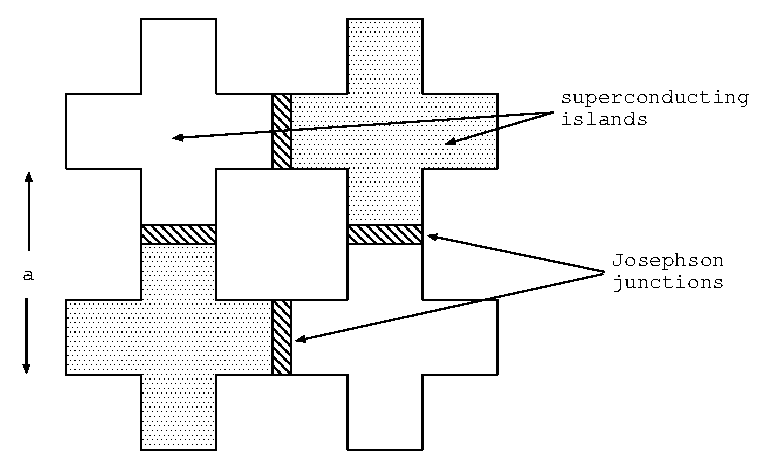
\includegraphics{figs/jjarray/fig1.eps}
\caption[One plaquette of a \jja.]{One plaquette of a \jja. The 
cross shaped islands of superconductor are in two layers 
(white and speckled). At the cross overlap a junction is formed
(cross-hatched region). The unit cell size is $a$. }
\label{fig:array_realization}
\end{figure}

\section{Single plaquette of Josephson-junction array}
\label{sec:single_loop}

Before analyzing the entire array in detail, I consider
the constitutive elements of the array: superconducting islands
joined by weak links, shown in \FigRef{fig:array_realization}.
The simplest component of the array is a single plaquette, a loop,
which 
for our arrays consists of four \jjsnoun, but in general may consist of
$N$ \jjsnoun. 
By looking at a single loop we can begin to 
directly compare experiment and 
analytical results. By contrast a
n entire array may only be solved numerically, 
even though the equations are known. 
Additionally, remnants of the single loop behavior may be seen
at the level of the entire array
\cite{ebner_prb_31_165_1985,deleo_unpublished}, 
so an understanding of the single-loop 
will be important to aid in understanding the entire array. 
Indeed the single-loop model has been used
many times in the literature in an attempt to explain phenomena
primarily associated with the paramagnetic Meissner effect
\cite{auletta_physc_235_3315_1994,araujo_prl_78_4625_1997,%
barbara_prb_60_7489_1999,sigrist_jpsj_61_4283_1992,sigrist_rmp_503_67_1995}. 

%
% fig2.2-- schemtic of RCSJ model
%
\begin{figure}[p]
\includegraphics{figs/jjarray/fig2.eps}
\caption[Circuit schematic of single \jjnoun.]{A schematic showing the 
various elements which go into 
modeling a single \jjnoun\ in the RCSJ model. 
The $\times$ represents the Josephson element,
while a resistive and a capacitive channel shunt the junction. The current
through the junction would be measured as indicated.} 
\label{fig:single_junction_sketch}
\end{figure}

\subsection{RCSJ model}
\glossary{RCSJ}
\index{RCSJ model|(emph}

\FigRef{fig:single_junction_sketch}\ shows the simple circuit 
model commonly used to model a single \jjnoun\footnote{See Tinkham
\cite{tinkham}, p.~206 
or Newrock \etal \cite{newrock_ssp_54_263_2000}, p.~275.}
This represents
the so called Resistively and Capacitively Shunted Junction (RCSJ) model
of a \jjnoun,  
with a capacitive channel resulting from the physical overlap between the 
two islands of superconductor and a resistive channel due to quasiparticle
tunneling. The third channel, the $\times$, represents the Josephson
channel which obeys the Josephson relations
\cite{josephson_pl_1_252_1962}
\index{Josephson relations}
%
% Josephson equations
%
\begin{eqnarray}
I & =&  I_c \sin\gamma \\
V & = & {\Phi_0\over 2\pi}{\dif\gamma\over\dif t}
\end{eqnarray}
%
in which $I$ is the current through the junction, $I_c$ is the critical
current of the junction,  $V$ is the voltage across the junction
and $\Phinot$ is the flux quantum.
The parameter $\gamma$ is the gauge-invariant phase difference across
the junction, defined as
\index{gauge invariant phase difference}
%
\begin{equation}
\gamma = \Delta\varphi - 
       {2\pi\over\Phinot}\int \vec A \cdot \dif\,\vec\ell
\end{equation}
% 
where $\Delta\varphi$ is the difference in the phase of the superconducting
order parameter across the junction, $\vec{A}$ is the vector potential
through the junction and the integral is taken from one side of the 
junction to the other.
If the capacitance can be neglected
the model reduces to the so-called Resistively
Shunted Junction (RSJ) model.\footnote{See Tinkham \cite{tinkham} p.~202 
or Newrock \etal \cite{newrock_ssp_54_263_2000} p.~275.}%
\index{RSJ model}%
\glossary{RSJ}%  

In the RCSJ model the current $I$ through the junction, resistor and
capacitor must obey
%
% RSCJ current model 
%
\begin{equation}
\label{eqn:RCSJ}
I = I_c \sin(\gamma) + {1\over R} {\Phi_0 \over 2 \pi}{\dif\gamma \over \dif t}
+ C {\Phi_0 \over 2 \pi} {\dif^2\gamma \over \dif t^2}
\end{equation}
%
where $R$ is the 
quasi-particle or shunt resistance and $C$ is the junction capacitance.  
Around a closed loop of superconductor,
fluxoid quantization holds
%
%  fluxoid quantization equation
%
\index{fluxoid quantization}
\begin{equation}
\label{eqn:fluxoidquant}
\sum_j \gamma_j = 2 \pi n - 2 \pi {\Phitot \over \Phinot }
\end{equation}
%
in which $j$ indexes each junction in the loop, $n$ is the quantization
number and $\Phitot$ is the total flux $\Phi$ threading the loop.
In addition the loop has a self inductance $L$ which relates
the total flux to the flux applied to the loop, \Phiext,
%
%
%
\begin{equation}
\label{eqn:ftotvsfext}
\Phitot = \Phiext + L I 
\end{equation} 
%
Here we have assumed that there is no external source of current,
so $I$ flows through each junction.
To simplify we assume that by symmetry 
all $N$ junctions in the loop are equivalent (we will discuss the asymmetric
case in the section on unidentical junctions, 
section \ref{sec:unsymmetric_junctions}) so 
that
%
%
%
\begin{equation}
\label{eqn:symmetry}
\gamma = {2 \pi\over N} \left(n -  {\Phitot \over \Phinot}\right)
\mathrm{.}
\end{equation}
%
For convenience we next transform our equations to a dimensionless
form with the substitutions \cite{cawthorne_prb_60_7575_1999}:
% 
\begin{eqnarray}
\betal & = & {2 \pi \over \Phinot} L I_c     \nonumber   \\
\betac & = & {2 \pi \over \Phinot} I_c R^2 C  \nonumber  \\
\tau    & = & {2 \pi \over \Phinot} I_c R t   \nonumber   \\
i       & = & I / I_c                       \nonumber \\
\phitot & = & \Phitot / \Phinot             \nonumber \\
\phiext & = & \Phiext / \Phinot \mathrm{.}
\label{eqn:dimensionless_subs}
\end{eqnarray}
%
We apply these substitutions to (\ref{eqn:RCSJ})-(\ref{eqn:symmetry})
to obtain a single dimensionless equation,
%
%
\begin{equation}
\label{eqn:ode}
\phitot  = \phiext + {\betal \over 2 \pi} \left\{
         \sin\left[{2 \pi \over N} (n - \phitot)\right]
        - {2 \pi \over N} {\dif \phitot \over \dif \tau} 
        + \left( {2 \pi \over N} \right)^2 \beta_c {\dif^2 \phitot \over \dif \tau^2}
        \right\}
 \mathrm{,}
\end{equation}
%
%
which is a second order differential equation in time.%
\footnote{Eqn.~\EqnRef{eqn:ode} has no $\dif n /\dif \tau$ 
term because $n$ is a 
discrete variable.} The time evolution of $\gamma$ and $n$ can be quite
complicated and will be discussed 
shortly. 

The analysis of 
\EqnRef{eqn:ode} proceeds in two different cases, that in which \phiext\ is
a constant or that in which \phiext\ is a function of time. To relate
to our experiments we will concern ourselves primarily with
the former, where $\dif\phiext / \dif\tau = 0$. 
For the RSJ model the last term in \EqnRef{eqn:ode}\ drops out,
reducing the equation to a first order differential equation
in time, greatly
simplifying the analysis. 
\index{RCSJ model|)}

\subsection[The meaning of the quantum number $n$]
{The meaning of the quantum number $\mathbf{n}$}
\index{$n$|see{quantum number}}
\index{quantum number|(emph}

Before continuing further we must discuss the meaning and 
importance of the quantum number $n$. The importance of this cannot
be over-stressed because there has been a tendency in the literature
to ignore the quantum number by setting $n=0$ 
(see \eg\ \InLineRef{dominguez_prl_72_2773_1994}).%
\footnote{A useful discussion of the proper definition of $n$ is given
in the appendix of \InLineRef{geigenmuller_prb_47_348_1993},
which reaches similar conclusions to those drawn here, through
slightly different means.}
Consider a solid loop of superconductor, 
at any given point, the value of the
order parameter (\cf\EqnRef{eqn:orderparameter}) must be single valued.
This requires that 
%
\begin{equation}
\label{eqn:solidloopintegral}
\oint\nabla\varphi \cdot \dif\vec\ell = 2\pi n ,
\end{equation}
%
with the 
integral taken around any closed path enclosing the center of the loop.%
\footnote{This is not the rigorous definition, but serves for the present
purpose (it is a special case) with minimal confusion.} 
%The expectation 
%value of the order parameter is proportional to the superfluid density,
%which is an observable and must be a fixed quantity.
If $n=0$, $\varphi$ remains unchanged after going around the loop.
If $n\ne 0$, $\varphi$ has changed by $2 \pi n$ after going around
the loop.

Now consider taking the solid superconducting loop and breaking it
to add a \jjnoun. 
We have to modify \EqnRef{eqn:solidloopintegral}\
to take into account this break in the loop. After 
accounting for any flux in the loop we obtain
%
\begin{equation}
\gamma = 2\pi n - {2\pi\over\Phinot}\oint \vec{A}\cdot\dif\vec\ell \mbox{,} 
\end{equation} 
%
the one-junction analog of \EqnRef{eqn:fluxoidquant}. 

One very interesting thing has happened: we have abstracted the quantum 
number away from a superconducting loop property to instead apply only
to the gauge invariant phase difference across the
\emph{junction}. 
Suppose a single fluxoid enters the loop, one of two things can 
happen, $n$ can increase by one or $\gamma$ decreases by $2\pi$. 
Either results in the 
same effect: balancing the increase in 
$\oint\vec{A}\cdot\dif\vec\ell$. 
The implication of this is clear for 
modeling the array: choose either $-\infty<\gamma<\infty$ 
and fix $n$, or limit $0 \le\gamma < 2\pi$ and increment
$n$ whenever $\gamma$ reaches its limits. 

There are multiple equivalent ways to choose starting 
values of $\gamma$ and $n$ for a numerical
model. 
Two equivalent starting values (primed and unprimed) will
always be related through
%
\begin{eqnarray}
n'      & = & n - (\gamma \,\bmod\, 2\pi) \nonumber \\
\gamma' & = & \gamma - 2 \pi n
\end{eqnarray}
%
For example
$n=0$ and $\gamma=-2\pi$ is equivalent to $n'=1$ and $\gamma'=0$.

As we allow the model to evolve in time 
we now have the choice to fix $n$ and 
allow $\gamma$ total freedom, or restrict $0< \Delta\gamma\leq 2 \pi$ 
and increment $n$.

For a loop with more than one junction, things become somewhat trickier
since the gauge invariant phase difference across each junction 
need not in general be the same
(a point conveniently neglected in \EqnRef{eqn:symmetry}), though the
quantization rule, \EqnRef{eqn:fluxoidquant}, must still be obeyed for 
the entire loop. To illustrate this point, consider the following 
scenario with symmetric junctions \ala\ \EqnRef{eqn:symmetry}:
$\betal \gg 1$, $N>1$ and  compare $n=0$ and $n=1$ for $\phiext = 0$.
Different results occur, $\phitot = 0$ or $\phitot > 0$. \emph{By 
fixing the value of $n$ we cannot access all of the possible 
solutions.}

%
% figure 2.3
%
\begin{figure}[p]
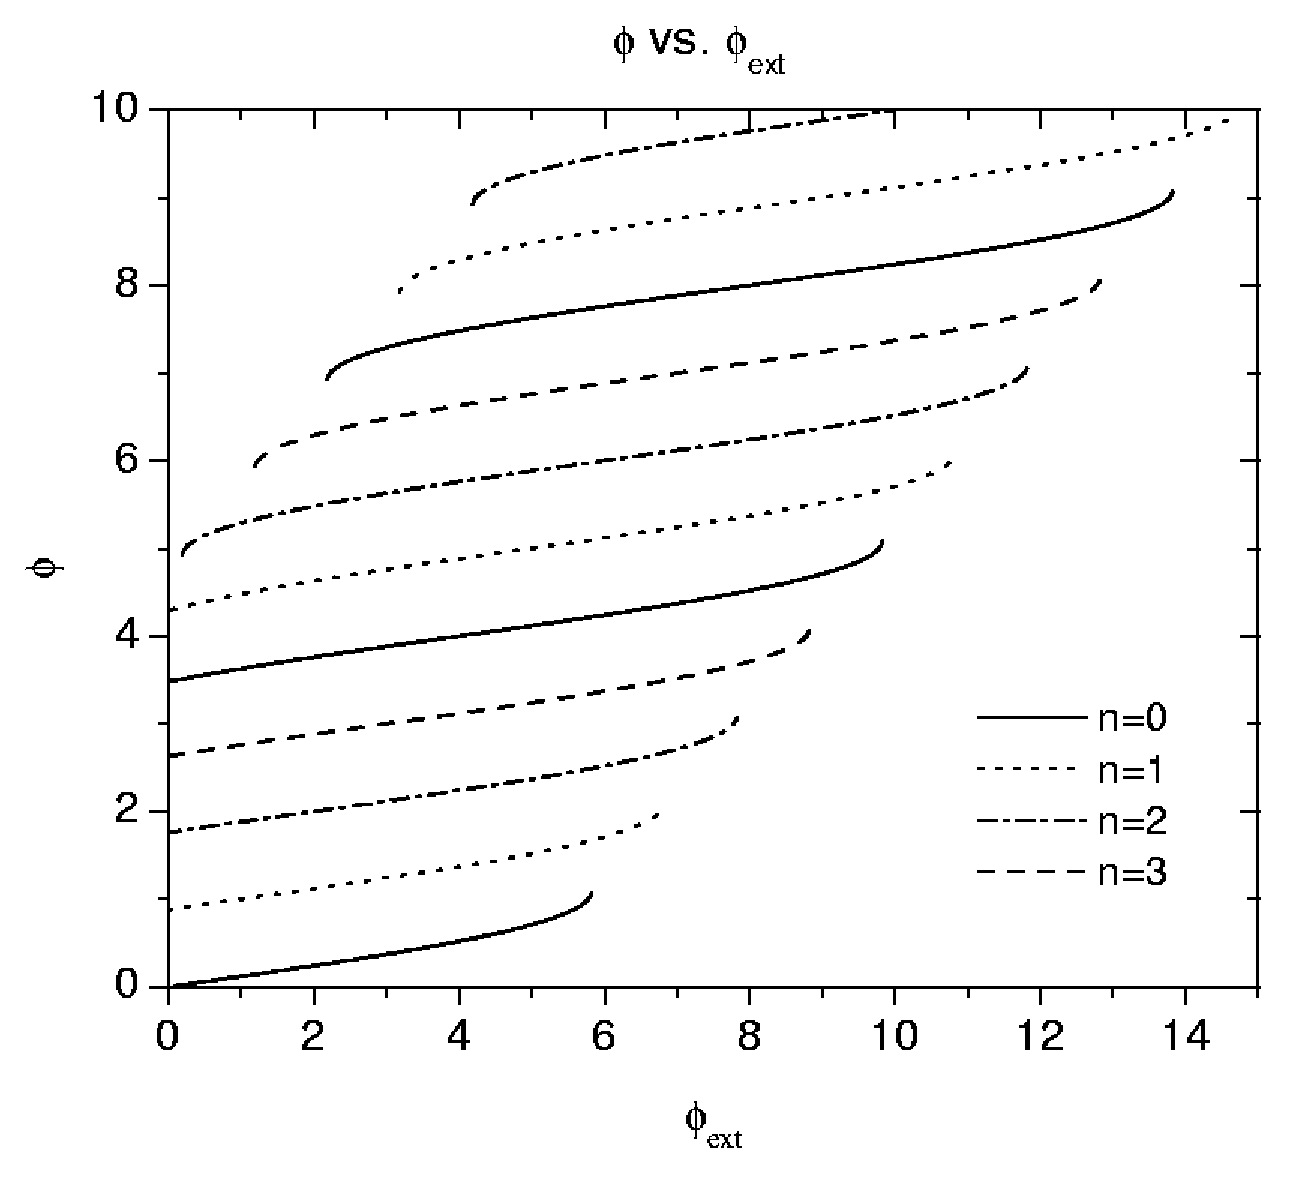
\includegraphics[width=5.7in]{figs/jjarray/chap2fig3.ps}
\caption[\phitot\ plotted against \phiext\ for $\betal= 30$
and $N=4$ for different values of the quantization number $n$.]
{\phitot\ plotted against \phiext\ from
\protect\EqnRef{eqn:steadystatesolution}\ for $\betal= 30$
and $N=4$ for different values of the quantization number $n$.
}
\label{fig:steady_state_multivariate_solution}
\end{figure}

\index{quantum number|)}

\subsection{Time independent external field}

To analyze 
\EqnRef{eqn:ode} we perform the standard stability analysis
\cite{ott} to find
that steady state solutions take the form of 
%
\begin{equation}
\label{eqn:steadystatesolution}
\phitot = \phiext + {\betal \over 2 \pi} \sin \left[{2 \pi \over N} (n -
                           \phitot) \right]
\mathrm{.}
\end{equation}
%
The right hand side can result in either single or multiple solutions,
depending upon the value of \betal. The crossover point depends 
upon $N$, and the solutions are single-valued for $\betal < N$ and
multi-valued for $\betal \geq N$. 
\FigRef{fig:steady_state_multivariate_solution}\ shows 
\EqnRef{eqn:steadystatesolution}\ plotted for large $\betal= 30$
which demonstrates that for a given \phiext\ there are many different
solutions for \phitot\ possible. The solutions for different values
of $n$ are sometimes referred to as the different ``branches'' of the
solution. For each of these branches, only the positively sloped 
parts are plotted, because these are the physically realizable solutions,
which will be discussed below. 

\subsubsection{$\pi$-junctions}
\index{\pijunction|(emph}
\label{sec:pijunction}

Another interesting possibility is the presence of an intrinsic 
phase shift in
the order parameter across the junction. This phase shift may occur
if \eg\ the junction is formed from misaligned grains of a superconductor
with \dwave\ symmetry. If the intrinsic phase shift across 
all the junctions sums to
$\pi$, \EqnRef{eqn:steadystatesolution}\ becomes modified to
%
\begin{equation}
\phitot = \phiext + {\betal \over 2 \pi} \sin \left[{2 \pi \over N} (n -
                           \phitot) - \pi \right]
\mathrm{.}
\label{eqn:steadystatepijunction}
\end{equation}
% 
This effect is commonly described as due to the presence of \pijunctions.
The important physical difference between \EqnRef{eqn:steadystatesolution}\
and \EqnRef{eqn:steadystatepijunction}\ is that at $\phiext = 0$,
\EqnRef{eqn:steadystatesolution}\ allows the loop to have zero magnetization
while \EqnRef{eqn:steadystatepijunction}\ forces the loop to be
magnetized. 
These two cases have been confirmed experimentally in two junction
SQUIDs
\cite{mathai_phdthesis,mathai_prl_74_4523_1995}. 

\index{\pijunction|)}

\label{jjarray:single_loop_mag}
Instead of plotting \phitot\ \vs\ \phiext\ as in 
\FigRef{fig:steady_state_multivariate_solution} it is useful
to also consider a plot of the normalized  
magnetization $\phimag = \phitot - \phiext$
\vs\ \phiext\ since it is the magnetization that is often measured
experimentally. This is shown in \FigRef{fig:single_loop_mag}. 
If we consider \EqnRef{eqn:steadystatesolution},
immediately one important fact springs forth: the larger \betal\ the
steeper the magnetization curves. This implies that small variations
in the external flux may create large variations in the total flux
of the single loop. Furthermore, it is clear from \FigRef{fig:single_loop_mag}\
that the single loop is equally likely to be either paramagnetic
or diamagnetic over the entire range of \phiext. 

%
% figure phimag vs. phiexternal
%
\begin{figure}[p]
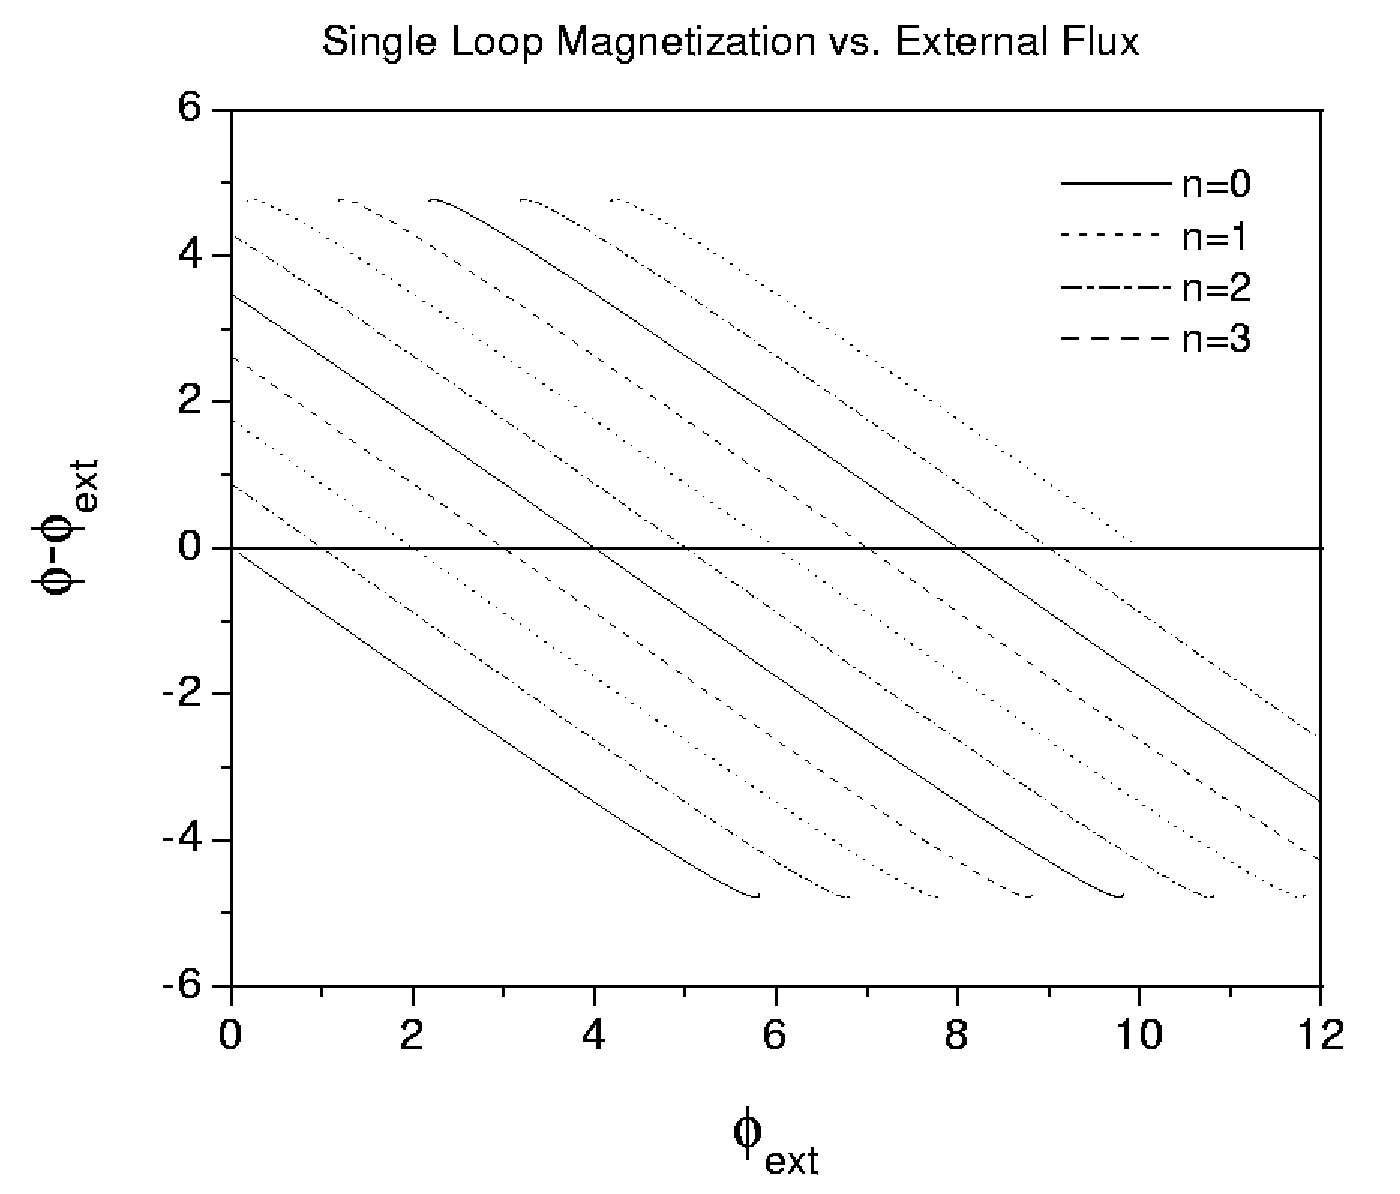
\includegraphics[width=5.7in]{figs/jjarray/phimag.ps}
\caption[Single loop magnetization \vs\ external flux.]
{Normalized magnetization
of a single loop, \phimag, plotted against the external flux \phiext\
applied to the loop for $\betal=30$ and $N=4$ for different values
of the quantization number $n$.}
\label{fig:single_loop_mag}
\end{figure}

Sigrist and Rice \cite{sigrist_jpsj_61_4283_1992,sigrist_rmp_503_67_1995}\
discussed the differences between
\EqnRef{eqn:steadystatesolution}\ 
and \EqnRef{eqn:steadystatepijunction}\ \visavis\ \swave\ and \dwave\ 
superconductivity for $N=1$ and concluded that observation of paramagnetism 
at $\phiext = 0$ provided evidence of a \pijunction\ in the
loop. However, they failed to account for the possibility that 
$\betal \gg N $ in \EqnRef{eqn:steadystatesolution}\ in which case
there are possible paramagnetic (and diamagnetic) 
solutions for \phitot\ at  $\phiext = 0$ even in the absence of 
\pijunction s. 

\EqnRef{eqn:steadystatesolution} does not tell the entire story.
For $\betal>N$ it specifies a multivalued solution with both
positive and negative slope. The solutions with positive slope are
seen experimentally, while those with negative slope are never seen.
This can be understood
by continuing the stability analysis of \EqnRef{eqn:ode}. 

%
% RSJ stability analysis
%
\label{RSJ model!stability analysis}
In the case of the RSJ model, \EqnRef{eqn:ode}\ reduces to 
%
\begin{equation}
\label{eqn:ode_rsj}
\phitot  = \phiext + {\betal \over 2 \pi} \left\{
         \sin\left[{2 \pi \over N}( n - \phitot)\right]
        - {2 \pi \over N} {\dif \phitot \over \dif \tau} 
        \right\}
\end{equation}
%
whose Jacobean has a single eigenvalue\footnote{For a complete discussion
of the stability analysis, see Ott \cite{ott}, p.~108.}
 of 
%
\begin{equation}
\label{eqn:rsj_eigenvalue}
\lambda =- {N\over 2 \pi} \left\{{2\pi\over\betal} + 
          {2\pi\over N} \cos \left[{2\pi\over N} (n-\phitot) \right] 
          \right\}
\end{equation}
%
For $\betal < N$, $\lambda$ will always be negative, hence any direction in 
\phitot\
from \EqnRef{eqn:ode}\ is a stable direction. This means that the loop
can settle into any value of \phitot\ for a given \phiext which 
solves \EqnRef{eqn:ode_rsj}. Additionally,
the solution to 
\EqnRef{eqn:ode_rsj}\
is single valued, so there is no ambiguity as to the state of the loop. 

In the case when $\betal > N$, $\lambda$ may change sign depending upon 
the particulars of the situation and $\lambda$ will be negative for 
%
\begin{equation}
\label{eqn:overdampedattracteigenvalue}
\cos\left[(n-\phitot) {2 \pi \over N} \right] > -{N \over \betal}.
\end{equation}
%
For $\lambda < 0$ the directions from the fixed point solutions
are stable directions so that the loop will stay in such a configuration. 
When $\lambda > 0$ the directions are unstable;  should any small thermal
fluctuation occur, a loop on the unstable 
fixed point solution will leave, and be
driven even further from the unstable solution. 


To illustrate this point, consider the first time derivative of 
\EqnRef{eqn:ode_rsj},
\begin{equation}
-\left\{1+{\betal\over N}\cos\left[(n-\phitot){2\pi\over N}\right]\right\}
{\dif\phitot\over\dif\tau} = {\betal\over 2\pi}{\dif^2\phitot\over\dif\tau^2}
\end{equation}
which takes the form of a moving particle experiencing a drag force. 
The ``drag coefficient''
\begin{displaymath}
-\left\{1+{\betal\over N}\cos\left[(n-\phitot){2\pi\over N}\right]\right\}
\end{displaymath}
takes a special form that is dependent upon \phitot, the position variable. 
Additionally,
the drag coefficient changes sign:  Instead of exerting drag, 
and slowing the particle, it pushes the particle and accelerates it 
away from \phitot. 
Conversely, when the drag 
coefficient is negative, the particle slows toward \phitot. The condition
for this switch over occurs at exactly the same place as the switch over
described for the eigenvalues above. 


%
% RCSJ stability analysis
%
\index{RCSJ model!stability analysis}
In the case of the RCSJ model, including $\betac$ in
\EqnRef{eqn:steadystatesolution}, makes the eigenvalues of the Jacobean 
more complicated,
but the same underlying behavior given by 
\EqnRef{eqn:overdampedattracteigenvalue}
occurs. The difference is that now while solutions are still
attracting or repelling, there are two types, depending on whether
or not the eigenvalues are complex or real. 
The eigenvalues themselves are given by
%
\begin{equation}
\label{eqn:fulleigenvalues}
\lambda_\pm = {N \over 4 \betac \pi} \pm {N \over 4 \betac} 
        \sqrt{1 + 8 \pi {\betac \over  \betal}
               + 2 \pi \betac \cos \left(\phitot {2 \pi \over N} 
                     \right)}
\end{equation}
%
The eigenvalues will
be purely real when
%
\begin{equation}
\label{eqn:undrivenrealeigen}
\cos \left[ (n-\phitot) {2 \pi \over N} \right] > - {1 \over 2 \pi \betac} 
                                              - {N \over \betal}
\mathrm{.}
\end{equation}
%
For sufficiently small \betal\ and \betac\ the eigenvalues will always 
be real and there will only be stable directions to the fixed point.
Additionally \EqnRef{eqn:undrivenrealeigen}\ 
reduces to the previous results for over damped junctions, if 
$\betac \rightarrow 0$. For large
enough \betal\ and \betac\ the fixed point solutions will have two
unstable directions. There is a range in between these
two possibilities in which the fixed point solutions have one stable
and one unstable direction. The unstable direction always dominates
in \EqnRef{eqn:fulleigenvalues}\ and the fixed point is  a
repulsor. 


\subsection{Time-dependent external field}

The single loop may also be put into a time-varying external field. 
The simplest case which may be considered, and the only case considered
here, is that of a sinusoidal 
driving field
%
\begin{equation}
\label{eqn:sindrive}
\phi_\mathrm{ac}(\tau) = \phiext \sin (\omega \tau)
\end{equation}
%
%We can separate \EqnRef{eqn:ode}\ into three first order autonomous 
%equations, when we substitutute \EqnRef{eqn:sindrive}\ for \phiext. 
%These are:
%\begin{eqnarray}
%{\dif \phiext' \over \dif \tau} & = & {8 \over \pi \betal \betac} \times \nonumber \\
% & & 
% \left[ -\phitot +\phiext\sin(f)+{\betal \over 2 \pi} \sin 
%     \left({n \pi \over 2} - {\pi \over 2}{\phitot \over \Phi_0} \right)
%   - {\betal \over 4} \phitot' \right] \\
%{\dif \phitot \over \dif \tau} & = & \phitot' \\
%{\dif f \over \dif \tau} & = & \omega .
%\end{eqnarray}

We can substitute \EqnRef{eqn:sindrive}\ for \phiext\ in to
\EqnRef{eqn:ode}\ and then analyze the result in different cases. 
It is useful to make the definition
\begin{equation}
\omega_0^{-2} = {\pi\over 8}\betal\betac , 
\end{equation}
where $\omega_0$
 corresponds to the dimensionless natural frequency of the system
if the non-linear \jj\ term is ignored. 
To see why this definition of $\omega_0$ is useful, consider 
rewriting \EqnRef{eqn:ode} in the form
%
\begin{equation}
\label{eqn:ode_reform}
{\pi\over 8}\betal\betac {\dif^2\phitot\over\dif\tau^2} = 
-\phitot + \phiext\sin(\omega\tau)-{\betal\over 4}{\dif\phitot\over\dif\tau}
+ {\betal\over 2\pi}\sin\left[ (n-\phitot){2\pi\over N} \right]
\end{equation}
%
which is clearly the form of a forced, damped harmonic
oscillator with an additional non-linear term. 


\subsubsection{Quasi-static case}

The quasi-static case is associated with $\phiext \ll {\betal/ 2 \pi}$ 
and 
$\omega \ll \omega_0$.
In this case the solutions are basically what we
expect for the static case. The system is driven so slowly and with such
low amplitude that it is always essentially in equilibrium. 
%There is no energy stored magnetically, all of the 
%energy is dissipated in the resistive channels in the junctions. 

%
% cut this section because I cannot justify it, nor do I think it's
% correct any longer. 
% 
%\subsubsection{Resonance}
%
%Resonance occurs when the driving frequency equals the natural
%frequency of the system $\omega_0 = \omega$. In this case, the non-linear
%term is irrelevant, and the loop operates essentially as a linear
%oscillator at resonance. 

\subsubsection{Large driving amplitude}

An interesting situation occurs when $\phiext \gg \betal / 2 \pi$. 
Here \phiext\ drives the loop so hard that the non-linear term is
irrelevant. This case corresponds to the loop responding simply as
a harmonic oscillator. 

\subsection{Gibbs free energy of single loop stable solutions}
\label{sec:gibbs_free_energy}

Assuming that the loop is able to achieve thermodynamic equilibrium
(which we have not generally assumed) the most favorable solution 
given by \EqnRef{eqn:steadystatesolution} would be the solution
\index{Gibbs free energy}
with the lowest Gibbs free energy. The Gibbs free energy in this case
is $\dif G = -I \dif\Phiext$\ \cite{silver_pr_157_317_1967,barone_and_paterno} 
which is easily determined 
numerically. 
This yields a series of Gibbs free energies for
each possible solution to \EqnRef{eqn:steadystatesolution}, with
the lowest Gibbs free energy corresponding to the solution which
has \phitot\ closest to \phiext. 
For the \phitot\ \vs\ \phiext\ curves in 
\FigRef{fig:steady_state_multivariate_solution} with $\betal = 30$, the
Gibbs free energy curves are plotted in
\FigRef{fig:gibbs_free_energy}.

\begin{figure}[p]
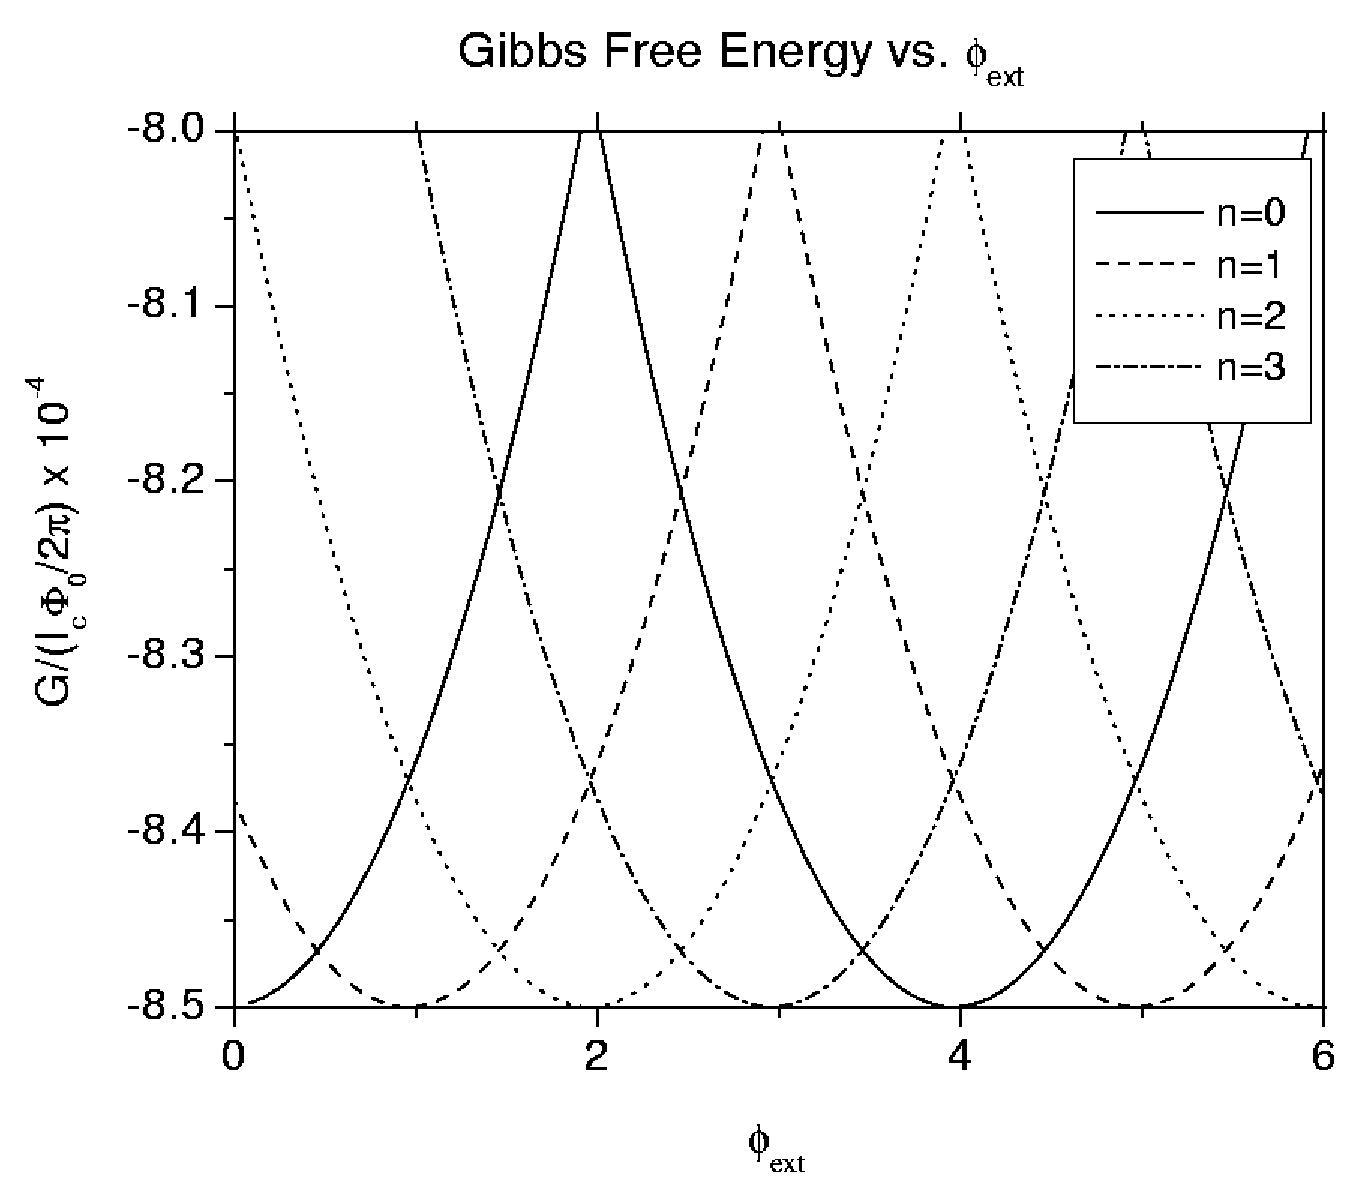
\includegraphics[width=5.7in]{figs/jjarray/chap2fig4.eps}
\caption{Gibbs free energy calculated for a four-junction loop with
$\betal = 30$.} 
\label{fig:gibbs_free_energy}
\end{figure}

\subsection{Non-identical junctions}
\label{sec:unsymmetric_junctions}

If we ignore the symmetry arguments which resulted in \EqnRef{eqn:ode}\
then for $N$ junctions in an isolated loop, for we will have $N$ equations to
solve. For each junction, \EqnRef{eqn:ftotvsfext} implies
%
\begin{equation}
{\phitot} = \phiext + {{\betal}_i\over 2 \pi} \sin \gamma_i
\label{eqn:ftotvsfext_indiv}
\end{equation}
%
in which ${\betal}_i$ is the $\betal$ parameter of the individual junction,
and accounts for individual junction variations in $I_c$ in the static 
case.  
In addition, the quantization rule, \EqnRef{eqn:fluxoidquant}, still holds.
We now substitute
\EqnRef{eqn:ftotvsfext_indiv} for 
\phitot\ to arrive at an equation for each junction, 
%
\begin{equation}
n-\phiext - {1\over 2\pi}\sum_i \gamma_i-{{\betal}_i\over 2\pi}\sin\gamma_i=0
\mathrm{.}
\end{equation}
%
The system must be solved numerically.
If one of the 
${\betal}_i$ is much larger than the others, then the loop behaves primarily
as a loop with $N-1$ junctions. For variance in ${\betal}_i$ on the order
of $10\%$, there is little change in the outcome, 
compared to the results for the
symmetric loop. 
This means that experiments on loops or \jjas\ with critical 
current
variations on the order of $10\%$ or less should exhibit behavior
similar to a uniform loop or array. Furthermore, models incorporating
uniform critical currents are significantly easier to implement.

This is significant because if small variations do not
affect the results very much, then
we expect that for a real \jja\ variations 
in the junction parameters on the order of $10\%$ will have only a small
bearing on the observations of those arrays. 

\section{Complete model of entire array}
\label{sec:entire_array_model}

% this figure shows the general outline for the array, including
% which junctions have which variables, etc. 
% this is a simple wire sketch, no islands etc. 
%
\begin{figure}[p]
\includegraphics{figs/jjarray/fig5.eps}
\caption[Sketch of \jja\ with labeled variables for numerical modeling.]
{Schematic arrangement for a square lattice \jja\ showing the 
variables used to describe each plaquette and junction in the
array. The positive direction for the loop currents are clockwise,
as indicated by the arrows, positive $\theta_{i,j}$ and $\gamma_{i,j}$
are measured in the vertical and horizontal direction respectively.}
\label{fig:array_model_sketch}
\end{figure}

To study the entire array, we take the same basic equations which describe
a single loop and scale them up.
In this section we will
consider a generic square lattice of $N \times M$ \jjsnoun, as depicted in 
\FigRef{fig:array_model_sketch}. \jjsnoun\ in the vertical
wires\footnote{The wires of the array are often refereed to as ``branches,''
while the loop currents are sometimes referred to as ``mesh'' currents.}
of the array are described by gauge-invariant phase difference 
$\theta_{j,k}$ and in the horizontal
wires by $\gamma_{j,k}$, while $I_{j,k}$ describes the loop current flowing
around each plaquette in the array. Considering loop currents simplifies
the analysis by eliminating the need to consider Kirchhoff's laws at each
intersection point of the array. 
For simplicity, consider here that the junctions are identical. 
With this arrangement, we may write an 
equation describing the current through each junction, using the normalizations
from the single loop case,
%
\begin{eqnarray}
\label{eqn:junc_horiz}
i_{j,k}-i_{j,k-1} & = & \sin\gamma_{j,k} +  {\dif\gamma_{j,k}\over\dif\tau}
                        + \betac {\dif^2\gamma_{j,k}\over\dif\tau^2} \\
i_{j,k}-i_{j-1,k} & = & \sin\theta_{j,k} + {\dif\theta_{j,k}\over\dif\tau} 
                        + \betac {\dif^2\theta_{j,k}\over\dif\tau^2} 
\label{eqn:junc_vert}
\end{eqnarray}
% 
as well as a quantization condition for each loop of the array,
%
\begin{equation}
\theta_{j,k} + \gamma_{j,k+1} - \gamma_{j,k} - \theta_{j+1,k} = 
 2 \pi n_{j,k} - 2 \pi \phi_{j,k} . 
\end{equation}
%
To fully define the array requires one further relation, the total flux
$\Phi_{i,j}$
threading the $i,j$ plaquette,
%
\begin{equation}
\phi_{j,k} = \phiext +{\betal\over 2 \pi} 
       \sum_{j',k'} m_{j,k,j',k'} \phi_{j',k'}
\label{eqn:total_flux_array}
\end{equation}
%
in which $m_{j,k,j',k'}$ is the mutual induction matrix between plaquette
$(j,k)$ and $(j',k')$ normalized to the self-inductance of a single plaquette,
$L$. 

The system detailed in Eqns.~(\ref{eqn:junc_horiz}) to 
(\ref{eqn:total_flux_array}) may also be condensed into a Hamiltonian
\index{Hamiltonian}
%
\begin{equation}
\mathcal{H} = \frac{1}{2}\betal 
           \sum_{j,k}\,m_{j,k,j',k'}\,{\phitot}_{j,k}\, i_{j,k}
    + \sum_{j,k} (1-\cos\gamma_{j,k})
    + \sum_{j,k} (1-\cos\theta_{j,k}),
\label{eqn:array_hamiltonian}
\end{equation}
%
where $\mathcal{H}$ is normalized to $\Phinot I_c / 2 \pi$. 
The sum in the first term is taken over each plaquette in the array while
the sums in the final two terms are taken over each junction in the array. 
This Hamiltonian will later be useful for investigating the energy 
landscape of the array. 

There have been many approaches to the solution of these equations
\cite{ebner_prb_31_165_1985,auletta_prb_47_14326_1993,%
auletta_prb_51_12844_1995,%
chandran_prb_56_6169_1997,%
filatrella_epjb_12_23_1999,lucheroni_prb_55_6559_1997} but perhaps
the most important result for the discussion here stems from work
by Phillips \etal \cite{phillips_prb_47_5219_1993}\ in which they 
show the importance of utilizing the full mutual induction matrix in order
to achieve accurate results. 

\subsection{Mutual induction matrix}
\index{induction matrix}

Because the full-induction matrix is just a geometrical property 
of the array it can in principle be computed. Phillips \etal\ put
forth one method to do this, on which this discussion will be based. 
There are two cases to consider when computing the matrix, the near
field, in which the physical extent of the plaquettes must be accounted 
for, and the far field, in which the plaquettes behave as current loops
composed of infinitesimal wires. 

\subsubsection{Near field}

We begin by modeling the array as a series of blocks (see 
\MultFigRef{fig:mutual_induction_matrix_blocks}{a}) and making 
the assumption
that the current density is uniform throughout the blocks.
Each block has
a uniform cross-sectional area $a$. The mutual induction matrix is then,
%
% the units of this are OK = Henry
\begin{equation}
\label{eqn:analytic_mutual_induction}
M_{j,k,j',k'} = {1\over a^2} {\mu_0\over 4 \pi} \oint\oint \dif\ell_{j,k}\,
  \dif\ell_{j',k'} 
  \int_A\int_{A'} {\dif a_{j,k}\, \dif a_{j',k'} \over \left|\vec r_{j,k} 
    - \vec r_{j',k'}\right|}
\end{equation}
%
which follows simply from Faraday's Law.\footnote{A very clear discussion
is given in Ramo, Whinnery and van~Duzer\cite{ramo_whinnery_vanduzer}, 
pp.~187-189.}
The integrals $\oint \dif\ell$ are taken around the two plaquettes 
of interest, the integrals $\int_A \dif a$ are taken over the facial area of
each block in the integration and $\mu_0$ is the magnetic constant.
\EqnRef{eqn:analytic_mutual_induction}\ 
cannot in general be integrated analytically, but can be integrated 
numerically
for the plaquettes of interest. 

%
% fig 2.6 -- geometry for mutual induction matrix
% 
\begin{figure}[p]
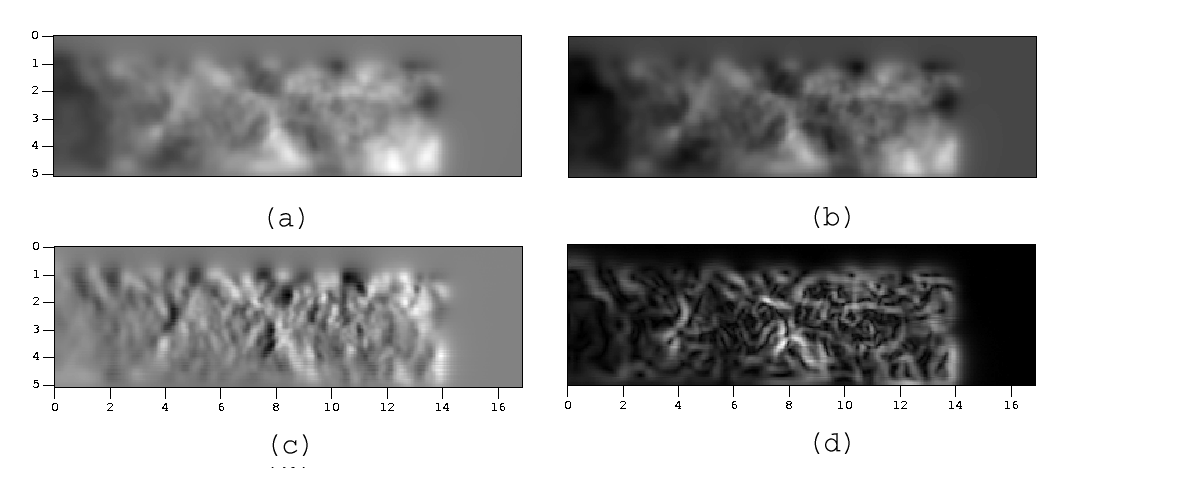
\includegraphics[width=5.7in]{figs/jjarray/fig6.ps}
\caption[Block arrangement used to compute mutual induction matrix.]
{Schematic of the block arrangement used to compute the
mutual induction matrix. (a) indicates the arrangement used for the 
near field, with $a_i$ representing the face of the block being
integrated over, $\ell_i$ representing the length around the loop 
integrated over, and $r$ representing the radius vector between the 
two blocks in the integration. (b) indicates the arrangement used 
to compute the mutual inductance in the far field. $r$ represents the
radius vector between the two loops and $\dif\ell_i$ represents the direction
of the integration around each loop.}
\label{fig:mutual_induction_matrix_blocks}
\end{figure}

\subsubsection{Far field}

In the far field \EqnRef{eqn:analytic_mutual_induction}\ simplifies
greatly to, as shown in \MultFigRef{fig:mutual_induction_matrix_blocks}{b},
%
% units of this equation are correct = Henry
\begin{equation}
M_{j,k,j',k'} = {\mu_0\over 4 \pi} {16 \sqrt{p} \over \sqrt{(j-j')^2 + (k-k')^2}}, 
\end{equation}
%
in which $p$ is the area of the plaquette,
which may be computed in a straight forward manner. 

It is complicated to compute the mutual induction matrix, but for a given
problem
we only need to compute the mutual induction matrix once.


% moved mean filed theory section to pme_theory.tex




% 29 May 2001 
%	comments from Chris
% 30 May 2001 with comments from Fred
% 30 May 2001 with comments from Paola
% 30 May 2001 with comments from R. Gomez

\chapter{Paramagnetic Meissner effect in Josephson-junction arrays}
\label{chap:pme_experiment}

\section{Introduction}
\label{sec:pme_exp_intro}

\index{Meissner effect}
Type I superconductors traditionally behave as perfect diamagnets; this is
the Meissner
effect, first described by Meissner and Ochsenfeld
\cite{meissner_dn_21_787_1933}\ in 1933. This means that the magnetic
induction $\vec{B}$ inside a superconductor is always zero. Consequently the
magnetization of a superconductor in a magnetic field $\vec{H}$ is given by
(in MKS units)
\begin{equation}
\vec{M} = -  \vec{H}.
\end{equation} 
In general, perfect diamagnetism 
holds true up to a certain critical field $H_{c}$ 
at which the superconductor turns into a normal metal. 

\subsection[Paramagnetic Meissner effect in \hightc\ superconductors]
{Paramagnetic Meissner effect in $\mathbf{\hightc}$ superconductors}

Recently, experiments by Braunisch \etal\ 
\cite{braunisch_prl_68_1908_1992,braunisch_prb_48_4030_1993}\
demonstrated that 
the superconductor
$\mathrm{Bi}_2\mathrm{Sr}_2\mathrm{CaCu}_2\mathrm{O}_y$
(BSCCO) could be paramagnetic. 
\index{Wohlleben effect}
\index{paramagnetic Meissner effect}
This effect has variously been referred to as the ``paramagnetic Meissner
effect'' (PME)%
\glossary{PME} or the ``Wohlleben effect.'' The former has become 
accepted and will
be used here. 
It was
further argued, following the work of Sigrist and Rice
\cite{sigrist_jpsj_61_4283_1992,sigrist_rmp_503_67_1995},
that this paramagnetism provided 
evidence for \dwave\ superconductivity in BSCCO.
\index{\pijunction}% 
We discussed in section~\ref{sec:pijunction}, p.~\pageref{sec:pijunction}
that a \pijunction\ may cause a superconducting loop
to have a paramagnetic moment. A \pijunction\ would result from 
grain misalignment in a superconductor with a \dwave\ order
parameter.
After the publication
of Braunisch \etal, others began to report paramagnetism in 
\hightc\ superconductors. For example, Reidling \etal\ reported PME in 
$\mathrm{Y}\mathrm{Ba}_2\mathrm{Cu}_3\mathrm{O}_{7-\delta}$
\cite{riedling_prb_49_13283_1994}; Schliepe \etal\ in 
BSCCO\,\cite{schliepe_prb_47_8331_1993}; \"{O}nba\c{s}li \etal\ in 
$\mathrm{Hg}\mathrm{Ba}_2\mathrm{Ca}_2\mathrm{Cu}_3\mathrm{O}_x$ (HgCCO)
\cite{onbasli_pssb_194_371_1996}; and Okram \etal\  in
$\mathrm{Nd}_{2-x}\mathrm{Ce}_x\mathrm{Cu}\mathrm{O}_y$   (NCCO)
\cite{okram_jpcm_9_L525_1997}. 

\subsection[Paramagnetic Meissner effect in \lowtc\ superconductors]
{Paramagnetic Meissner effect in $\mathbf{\lowtc}$ superconductors}

The continuing reports of PME solely in \hightc\ materials bolstered the 
belief that PME resulted from \dwave\ superconductivity, until the report 
of PME in conventional thick niobium disks by Thompson \etal
\cite{thompson_prl_75_529_1995}, by Kost\'{\i}c \etal
\cite{kostic_prb_53_791_1996} and later in niobium thin films by
Terentiev \etal\,\cite{terentiev_prb_60_r761_1999}. 
Further Geim \etal
\cite{geim_nature_396_144_1998} reported 
PME in mesoscopic 
aluminum disks.
Since niobium and aluminum are known to be \swave, this
discredited the \dwave\ explanation
for PME and caused a public controversy.%
\footnote{See \InLineRef{thompson_prl_75_529_1995} and the 
post-publication comments in \InLineRef{rice_prb_55_11467_1997} 
and \InLineRef{kostic_prb_55_14649_1997}.} 

We measured $\mathrm{Nb}-\mathrm{Al}_2\mathrm{O}_3-\mathrm{Nb}$
\jjas\ in order to investigate this controversy.%
\footnote{The research results of this work on PME in \jjas\ have 
lead to several publications, Refs.~\cite{nielsen_rdv_75_1999,%
nielsen_physb_280_444_2000,nielsen_prb_62_14380_2000,deleo_unpublished}.}
It is well known that 
niobium \jjas\
have no \pijunctions. Additionally
\jja\ fabrication takes place lithographically so we have great
control over the design of the sample. 
Highly ordered samples can be made photolithographically
in contrast to many of the granular \hightc\ 
samples. This makes our defect occurrence, \eg\ $J_c$ 
variations, no more than 10\%. Additionally, measurements of AC
susceptibility by
Araujo-Moreira \etal\,
\cite{araujo_prl_78_4625_1997} and 
Barbara \etal\,\cite{barbara_prb_60_7489_1999} demonstrated 
that \jjas\ might exhibit
PME. 

\section{Our samples}
\label{sec:sample_description}

The \jja\ samples discussed here were fabricated at 
Westing\-house\cite{westinghouse}\ by Martin Forrester and consist of
unshunted
$\mathrm{Nb}-\mathrm{Al}_2\mathrm{O}_3-\mathrm{Nb}$ \jjsnoun\
in arrays of $30\times 100$ and $100 \times 150$ \jjsnoun.%
\footnote{The arrays come from batches 10 and 11 and are 
designated \texttt{JJA-10-30} for the $30\times 100$  and \texttt{JJA-11-150}
for the $100 \times 150$.} 
The array design is the same as described in the previous chapter 
(chapter~\ref{chap:jjarray}, p.~\pageref{sec:single_loop},
\FigRef{fig:array_realization}).
An optical micrograph of a few unit cells of the array is shown
in
\FigRef{fig:sample_sketch}. 
The unit cell
size of each array is $46\,\micron$ with a wire width of $10\,\micron$. 
The niobium film is $200\,\mathrm{nm}$ 
thick and patterned into two layers of 
crosses. At the cross overlap a \jjnoun\ of $5\,\micron$ by
$5\,\micron$
is formed.  The calculated self-inductance of each loop of four junctions
is $L=64\,\mathrm{pH}$ and the measured critical current density 
at $4.2\,\kelvin$ is $J_c = 600\,\mathrm{A}/\mathrm{cm}^2$.%
\footnote{See \InLineRef{jaycox_ieeetm_mag17_400_1981} for a discussion
of the self-inductance in this case.}
The unit cell size is comparable to the typical grain size seen in BSCCO 
samples \cite{braunisch_prl_68_1908_1992,braunisch_prb_48_4030_1993,%
kirtley_jpcm_10_L97_1998} which exhibit PME. 

%
% fig 3.1
%
\begin{figure}[p]
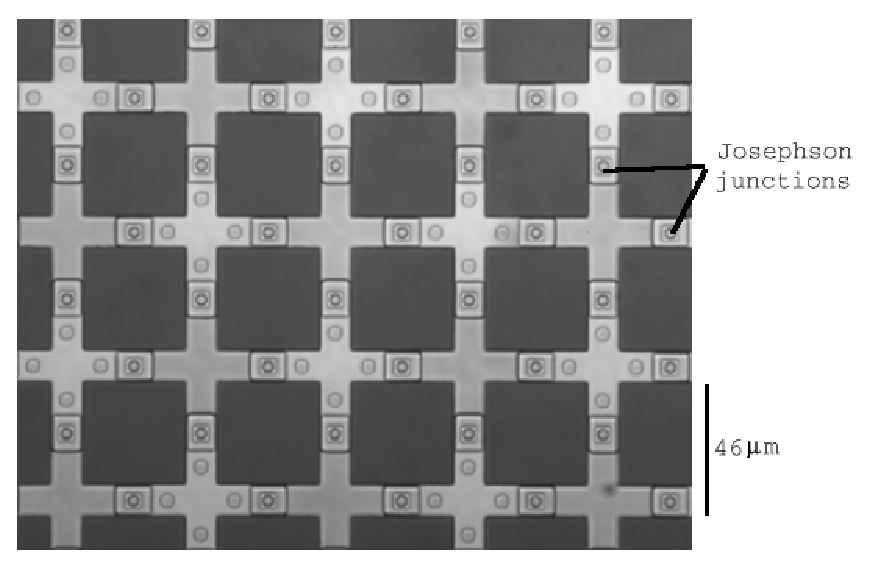
\includegraphics{figs/pme_exp/fig3_1.ps}
\caption[Optical micrograph of \jja\ samples used in the PME experiment.]
{Optical micrograph of several unit cells of the array showing
the crosses and locations of Josephson junctions. The unit cell size
is $46\,\micron$ and the wires are $10\,\micron$ across.
}
\label{fig:sample_sketch}
\end{figure}


\section{Experimental technique}
\label{sec:exp_method}

Kirtley \etal\,\cite{kirtley_jpcm_10_L97_1998}\ used a scanning SQUID
microscope (SSM), described in \InLineRef{kirtley_apl_66_1138_1995},
to image the BSCCO samples from Braunisch\etal 
\cite{braunisch_prl_68_1908_1992,braunisch_prb_48_4030_1993}\
and investigate the spatial distribution of paramagnetism in 
paramagnetic-superconducting BSCCO. This elegant experiment
provided inspiration for our work.

Our SSM has improvements over Kirtley's that make it ideally suited to
this type of experiment.\footnote{For a description of the 
experimental probe see
appendix \ref{chap:ssm_appendix}.} 
Our probe has a larger scanning 
range, as well as thermal isolation between the SQUID and the sample
(since they are not in direct contact).
 Kirtley \etal\ were unable to scan to the
edges of their sample, due to scanning stage restrictions. We are
able to scan over our entire sample, which proved to be crucial
to our analysis of the origin of PME. 
%Furthermore, there are artifacts
%in the Kirtley \etal\ data (\cf\ \InLineRef{kirtley_jpcm_10_L97_1998},\
%Fig.~1) due to the arrangement of the SQUID pickup coil which induces a
%false signal into the sample over the large area scanned. Because
%of our different SQUID arrangement we do not have this problem. 

The benefits of the SSM over more conventional magnetic measurement techniques 
are legion. The primary benefits arise from the fact that
the measured data are spatially resolved and the 
measurable field strengths are so low. 
Theories of PME
provide forms for the flux distribution
near the edges;%
\footnote{Theories of PME are discussed in the introductory material to
chapter \ref{chap:pme_theory}.} 
experimental verification
of these theories requires measurements of spatially-resolved magnetization. 
Other experimental techniques such as scanning Hall probe microscopy or
Magneto-Optical Indicator Films (MOIF) may be used to provide spatially
resolved information. However, both Hall probes and MOIF are not sensitive
to the magnetic field levels of interest in our arrays. 
One flux quantum per unit cell of the array has an average magnetic field
of $10^{-3}\,\mathrm{G}$ and we will typically measure 
signals on the order of
fractions of a single flux quantum. 

%
% fig 3.2
%
\begin{figure}[p]
\includegraphics{figs/pme_exp/fig3_2.eps}
\caption[Experimental arrangement of sample \jja\ and SQUID in the
probe.]{Experimental arrangement of sample \jja\ and SQUID at the cold
end of the scanning SQUID probe. The sample moves in $x$ and $y$
under the SQUID. Output signal from the SQUID is measured point by point
as the sample is scanned to generate an image of the magnetic induction
over the sample. The SQUID-sample separation is generally around 
$50\,\micron$. }
\label{fig:pme_experimental_setup}
\end{figure}

To run the experiment, \jja\ samples are placed on the end of the
cylindrical sample
stage cold finger, as shown in \FigRef{fig:pme_experimental_setup}. 
The cold finger is a $10\,\mathrm{mm}$ diameter sapphire 
rod around which a solenoid is wound. This solenoid provides the external
flux \Phiext\ to the sample. 

Prior to any measurement, the SQUID is adjusted
to insure that no flux is pinned in the body. This is accomplished by
first
thermal cycling the SQUID to remove trapped flux.  The
SQUID  is then scanned over a superconducting 
sample  (a technique developed in \InLineRef{mathai_phdthesis})
to observe if there is still
flux trapped in the SQUID, noting the sample 
response
as 
the SQUID is moved over the sample.
Eliminating the flux in the SQUID
minimizes the interaction between the SQUID and the sample and eliminates 
false signals that may result from
sample response to flux in the SQUID.

With the system cold,
we cannot easily know precisely how far apart the SQUID and the sample are.
To insure the SQUID does not collide with the sample, 
we rely on clues from the processed data. 
Sadly, many samples were lost due to the fact that 
the probe
provides no means to measure the separation \insitu. For a typical
scan discussed here, the SQUID -- sample separation is between
$40$ and $60\,\micron$. We infer this
because the lattice of the array is $46\,\micron$ and 
we can just begin to resolve array 
features in the data at this separation. For our
purposes we do not need to have unit cell resolution of the array,
nor will the exact measure of the SQUID -- sample separation affect the 
results. 

%
% somewhere we need to comment about the localization of the
% damage to the damaged regions... these pictures suck, so I'm cutting
% them out.
%
%It is important to not damage the array by allowing the 
%SQUID and sample to come into contact. \FigRef{fig:mag_array_scratches}\
%demonstrates the results of scratches accidentally introduced
%\insitu\ into the array,
%both in the magnetic image and also in the optical image, 
%\FigRef{fig:mag_array_scratches}(a) and (b) respectively, of the array. 
%Scratches destroy part of the array  affecting the magnetization
%properties of that part.

%
% figure was cut b/c the images were not clear. Instead I just say
% in the text what I tried to show with the images. 
%
% fig 3.3
%
%\begin{figure}
%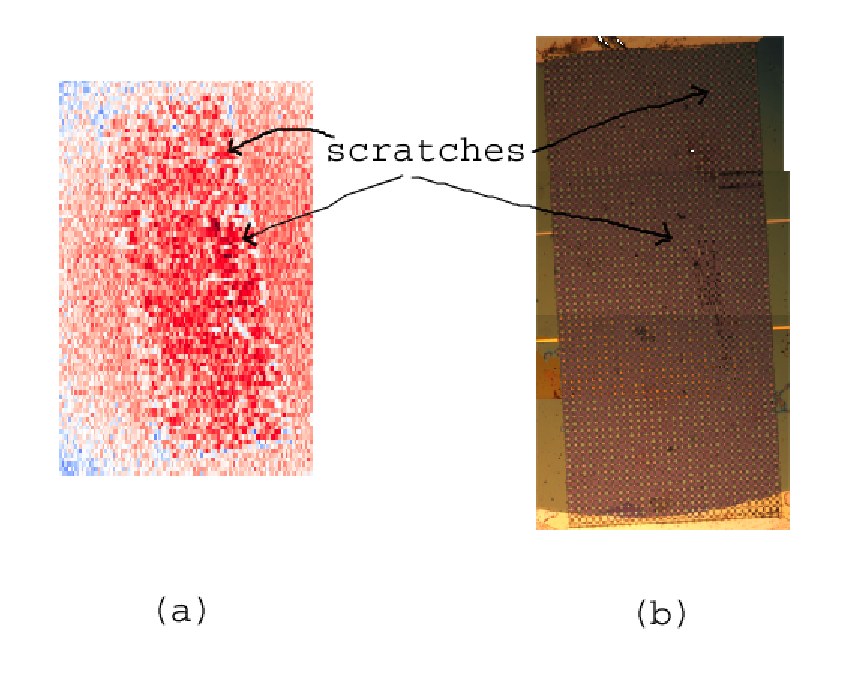
\includegraphics[width=5.7in]{figs/pme_exp/fig3_3.ps}
%\caption[Images of the $30\times 100$ junction array, 
%demonstrating \insitu\ scratches.]{(a) Magnetic image of the
%$30 \times 100$ junction array demonstrating accidental 
%\insitu\ scratches. (b) Optical micrograph of the same array
%showing the extent of the scratches.}
%\label{fig:mag_array_scratches}
%\end{figure}

After flux is removed from the SQUID, the sample is moved
so that the SQUID is far away (greater than
$10\,\mathrm{mm}$, in $x$ and $y$, not $z$) 
in order to 
avoid any possible interference between the SQUID and the sample during 
field cooling. \FigRef{fig:ZFC_with_close_SQUID} shows the effect of zero
field cooling the sample with the SQUID positioned over the middle of the 
$30 \times 100$ \jja. Flux became trapped in the sample in a similar pattern
to the wire arrangement on the surface of the SQUID tip, \cf\ 
\FigRef{fig:SQUID_optical_close}. 
It was found that turning off the SQUID, field cooling and
then reactivating the SQUID tended to trap flux in the sample when the 
feedback circuit was adjusted. 
To avoid this problem the SQUID was moved far away 
from the sample
until it had no noticeable effect when the sample was
zero field cooled.


% we want to arrange so that all color figures are on odd pages,
% or back to back, odd then even

\newcommand{\figthreefour}{
% in principle, this command will insert figure 3.4 right here
%
% fig 3.4 - color figure
%
\begin{figure}[p]
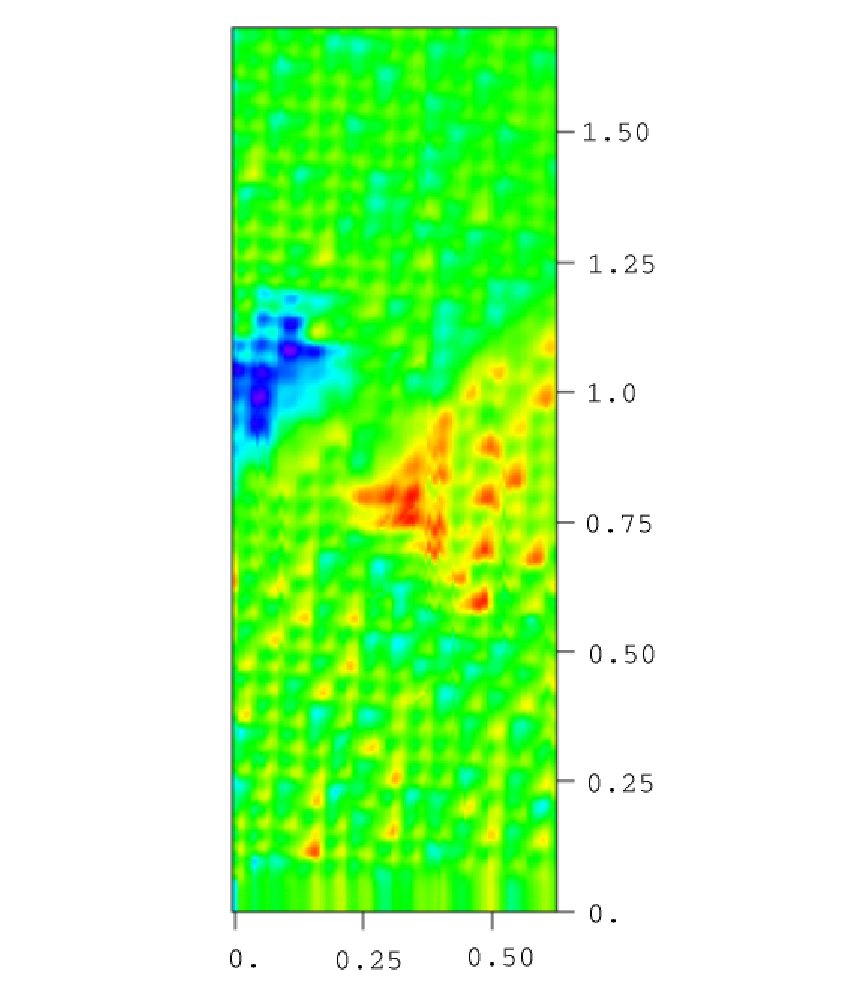
\includegraphics{figs/pme_exp/fig3_4r2.ps}
\caption[Zero-field cooled, with SQUID on top, magnetic image of sample.]{
Zero field cooled magnetic image of $30 \times 100$ \jja, with the 
SQUID positioned in the
middle of the sample during cooling. 
The color scale represents a range from purple (low) to red (high) of
$8 \Phinot$ per unit cell of the array and the $x$ and $y$ units are 
shown in millimeters. 
The flux trapped in the 
array is due to the currents flowing in the SQUID and feedback 
coil wires on the SQUID tip.
The smeared out data near $x=0$ is a mechanical artifact.} 
\label{fig:ZFC_with_close_SQUID}
\end{figure}
}

\ifthenelse{\isodd{\value{page}}}{\figthreefour}{\afterpage{\figthreefour}}

In practice, I begin taking measurements by
heating the sample above $T_c = 9.2\,\kelvin$
to $13\,\kelvin$. We then apply an external flux to the sample and remove
the heat source. The sample cools in field to $4.2\,\kelvin$ and the
measurement begins. 

Each measurement of a magnetization image 
consists of four scanning passes of the SQUID over the sample
in different situations.
Each scanning pass produces an image of the flux threading the SQUID at a 
particular point in space above the sample. 
\FigRef{fig:pme_scanning_passes_a} through 
\FigRef{fig:pme_scanning_passes_d}\ shows 
representative images of the four scanning passes made over the sample
to produce the magnetization image. 
We wish to compute the magnetization of the sample. In MKS units,
\begin{equation}
\vec{M}=\left( \vec{H}-{1 \over \mu_0} \vec{B} \right)\mathrm{.}
\label{eqn:magnetization_defn}
\end{equation}
The magnetization vector $\vec{M}$
can be related to a flux through an area
\begin{equation}
\Phimag = \mu_0 \int_A \vec{M}\cdot \dif \vec{a}
\end{equation}
just as $\vec{B}$ and $\vec{H}$ are associated with a flux through a 
particular area
\begin{eqnarray}
\Phitot & = & \int_A \vec{B}\cdot \dif \vec{a} \\
\Phiext & = & \mu_0 \int_A \vec{H}\cdot \dif \vec{a} \mathrm{.}
\end{eqnarray}
so that \EqnRef{eqn:magnetization_defn} can be expressed in terms of 
flux
\begin{equation}
\Phimag = \Phitot - \Phiext \mathrm{.}
\label{eqn:magnetization_flux_defn}
\end{equation}


%
% fig 3.5
%
%\begin{figure}[p]
%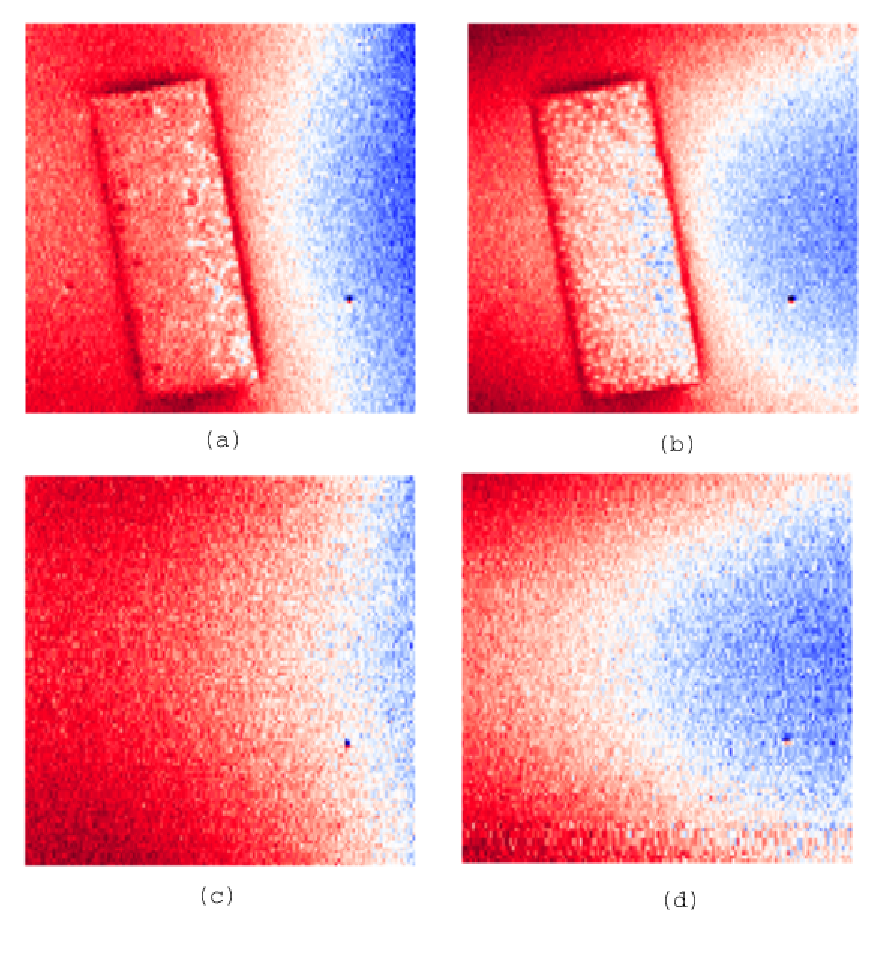
\includegraphics[width=5.7in]{figs/pme_exp/fig3_5r2.ps}
%\caption[Representative magnetic images from the four scanning passes
%required to determine the field cooled array magnetization.]{
%Representative images from the four scanning passes made in
%order to determine the magnetization of the field cooled sample.
%In each image the colors range from blue (low) to red (high) for 
%a total flux difference of $0.17\,\Phinot$ per unit cell of the
%array. Each image is $5\times 5\,\mathrm{mm}$ square. 
%(a) Magnetic image of sample after field cooling in $\phiext = 4.8$,
%$T=4.2\,\kelvin$.
%(b) Magnetic image of zero field cooled sample, $T=4.2\,\kelvin$. 
%(c) Magnetic image of $\phiext = 4.8$, $T=13\,\kelvin$. (d) Magnetic
%image of zero field, $T=13\,\kelvin$. }
%\label{fig:pme_scanning_passes}
%\end{figure}


\begin{figure}[p]
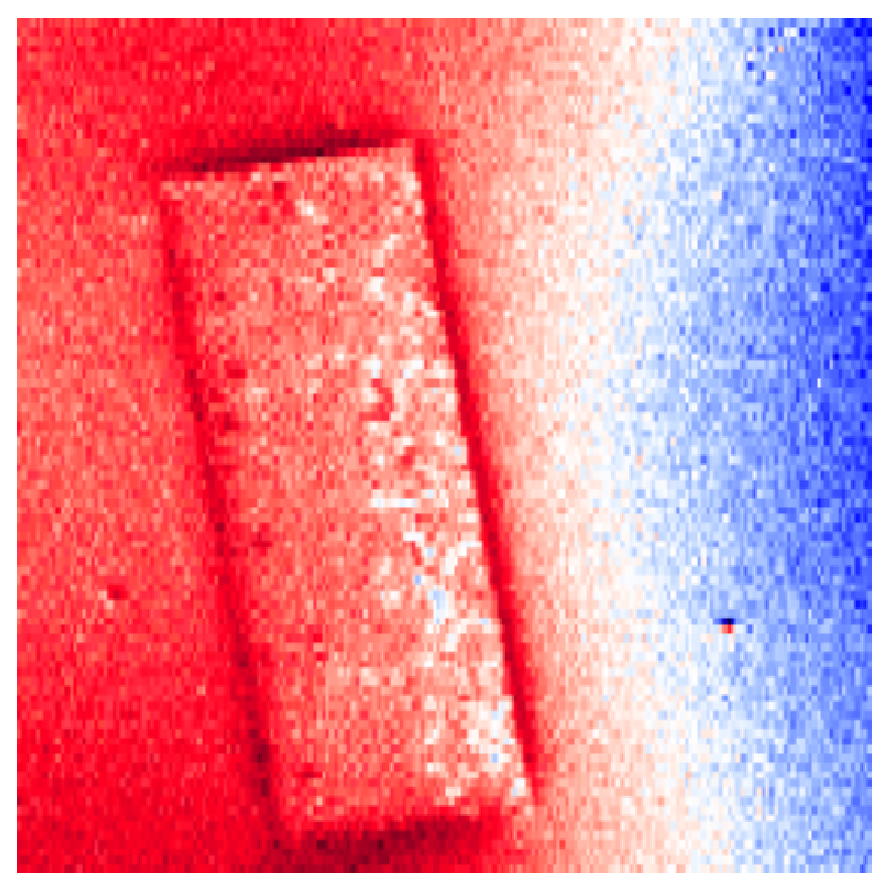
\includegraphics[width=5.7in]{figs/pme_exp/fig3_5_a_lg.ps}
\caption[Magnetic image of sample after field cooling in $\phiext = 4.8$,
$T=4.2\,\kelvin$.]{
Magnetic image of sample after field cooling in $\phiext = 4.8$,
$T=4.2\,\kelvin$.
The colors range from blue (low) to red (high) for 
a total flux difference of $0.17\,\Phinot$ per unit cell of the
array. Each image is $5\times 5\,\mathrm{mm}$ square.}
\label{fig:pme_scanning_passes_a}
\end{figure}

\begin{figure}[p]
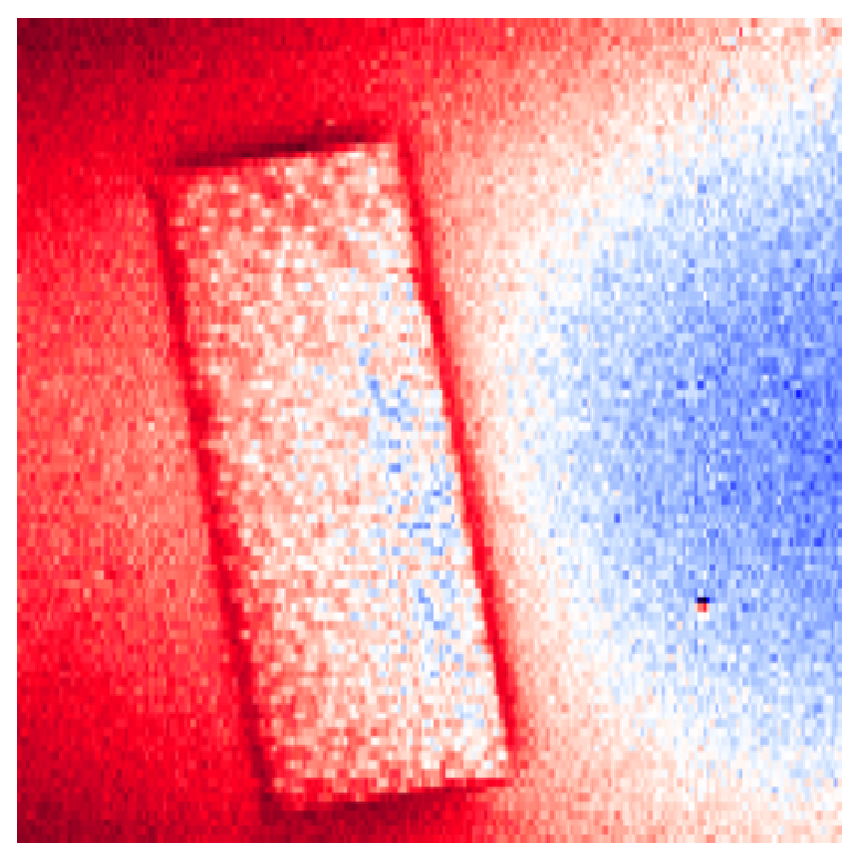
\includegraphics[width=5.7in]{figs/pme_exp/fig3_5_b_lg.ps}
\caption[Magnetic image of zero field cooled sample, $T=4.2\,\kelvin$.]{
Magnetic image of zero field cooled sample, $T=4.2\,\kelvin$.
The colors range from blue (low) to red (high) for 
a total flux difference of $0.17\,\Phinot$ per unit cell of the
array. Each image is $5\times 5\,\mathrm{mm}$ square.}
\label{fig:pme_scanning_passes_b}
\end{figure}

\begin{figure}[p]
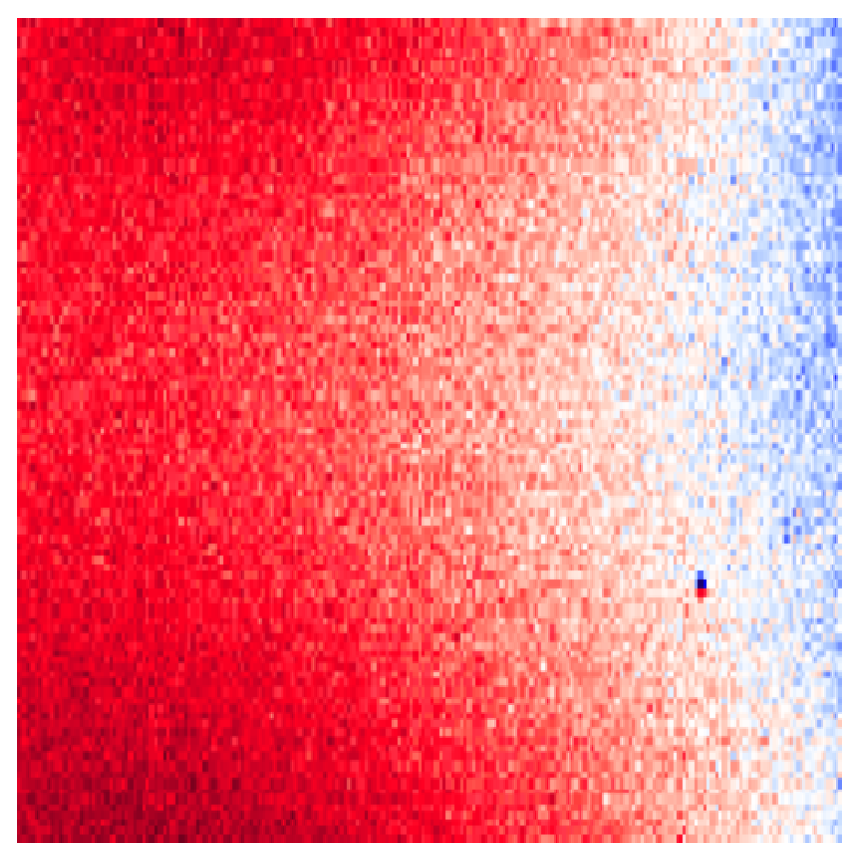
\includegraphics[width=5.7in]{figs/pme_exp/fig3_5_c_lg.ps}
\caption[Magnetic image of $\phiext = 4.8$, $T=13\,\kelvin$.]{
Magnetic image of $\phiext = 4.8$, $T=13\,\kelvin$.
The colors range from blue (low) to red (high) for 
a total flux difference of $0.17\,\Phinot$ per unit cell of the
array. Each image is $5\times 5\,\mathrm{mm}$ square.}
\label{fig:pme_scanning_passes_c}
\end{figure}

\begin{figure}[p]
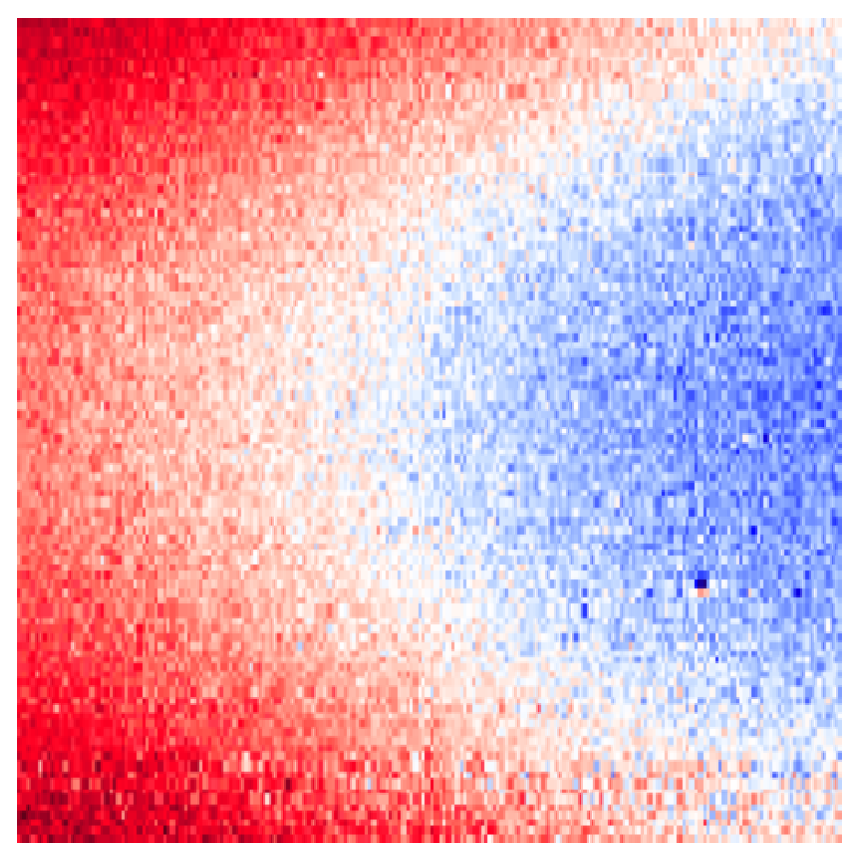
\includegraphics[width=5.7in]{figs/pme_exp/fig3_5_d_lg.ps}
\caption[Magnetic
image of zero field, $T=13\,\kelvin$.]{
Magnetic
image of zero field, $T=13\,\kelvin$. 
The colors range from blue (low) to red (high) for 
a total flux difference of $0.17\,\Phinot$ per unit cell of the
array. Each image is $5\times 5\,\mathrm{mm}$ square.}
\label{fig:pme_scanning_passes_d}
\end{figure}


%
% fig3.6
%
%\begin{figure}[p]
%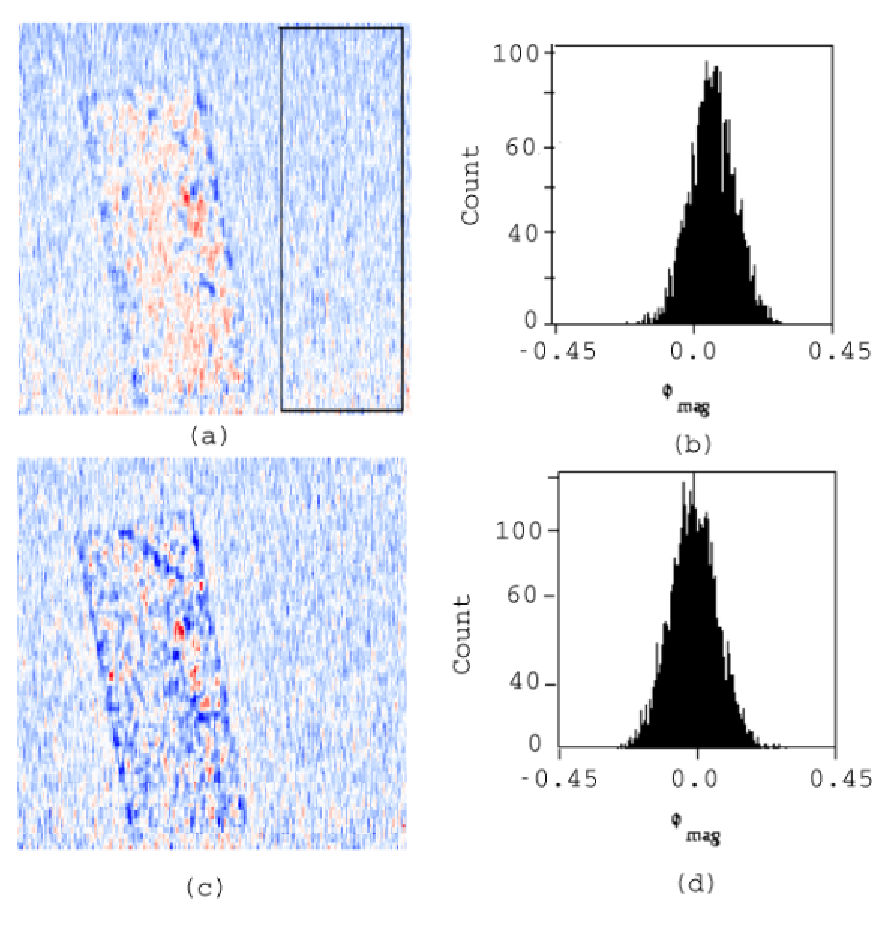
\includegraphics[width=5.7in]{figs/pme_exp/fig3_6.ps}
%\caption[Magnetization images of a field cooled $30\times 100 $ array.]{
%(a) Magnetization of $30\times 100$ junction array after field
%cooling in $\phiext = 4.8$. (b) Histogram of the magnetization data shown
%in the magnetization image (a). (c) Magnetization of array after field
%cooling in $\phiext = 1.2$. (d) Histogram of the magnetization data shown in 
%magnetization image (c). For both of the magnetization images the color 
%ranges from red, $\phimag = 0.45$ (paramagnetic) 
%to blue, $\phimag = -0.45$ (diamagnetic). The long side of the array
%is $4.6\,\mathrm{mm}$ long. 
%}
%\label{fig:paramag_image}
%\end{figure}

\begin{figure}[p]
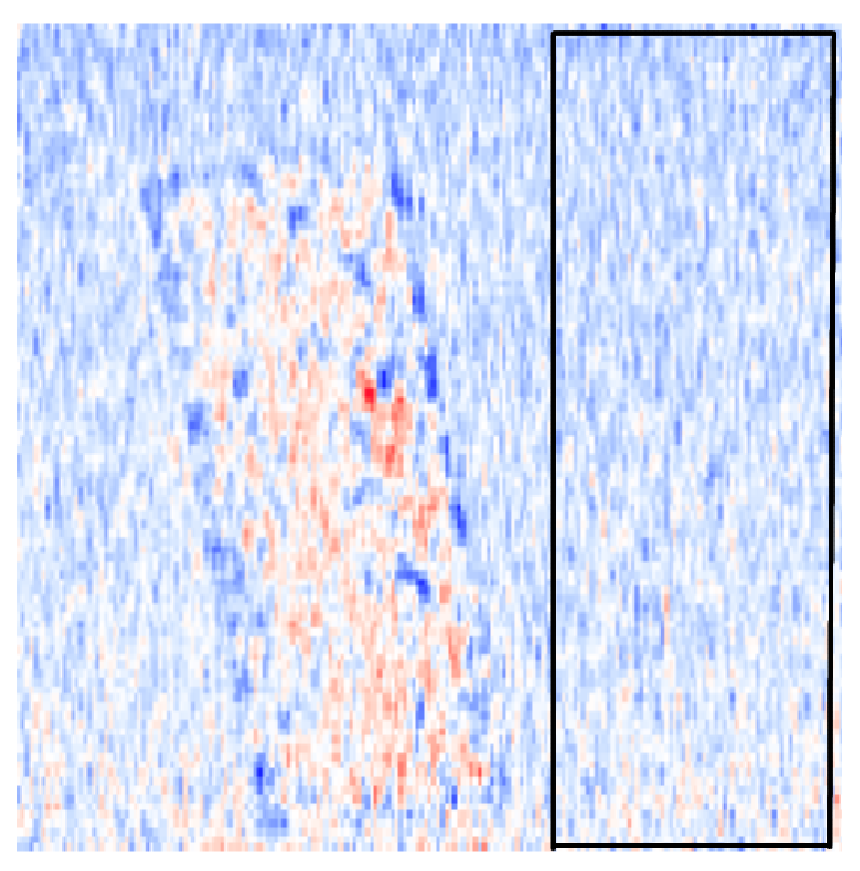
\includegraphics[width=5.7in]{figs/pme_exp/fig3_6_a_lg.ps}
\caption[Magnetization of $30\times 100$ junction array after field
cooling in $\phiext = 4.8$.]
{Magnetization of $30\times 100$ junction array after field
cooling in $\phiext = 4.8$. The color 
ranges from red, $\phimag = 0.45$ (paramagnetic) 
to blue, $\phimag = -0.45$ (diamagnetic). The long side of the array
is $4.6\,\mathrm{mm}$ long. }
\label{fig:paramag_image_a}
\end{figure}

\begin{figure}[p]
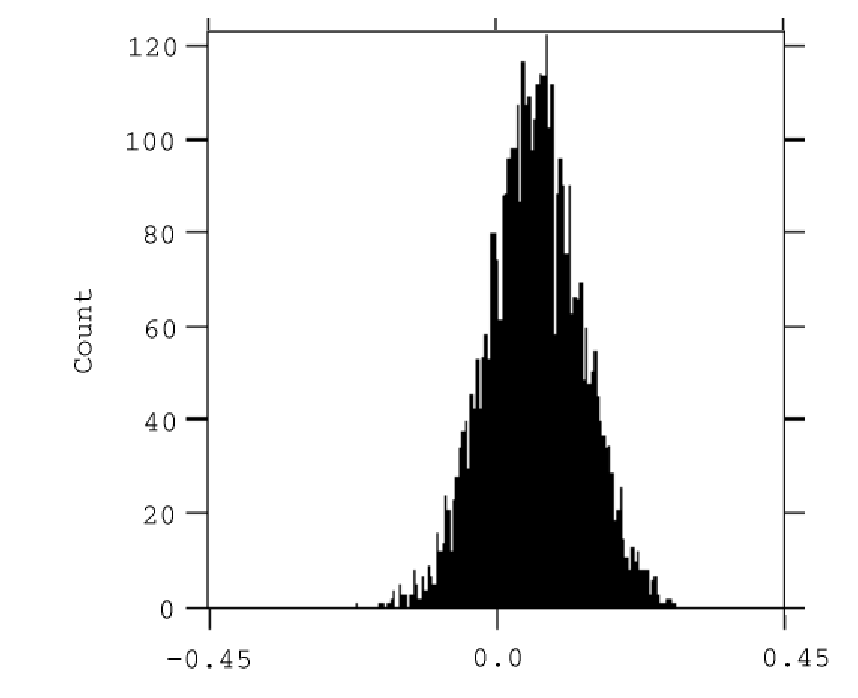
\includegraphics[width=5.7in]{figs/pme_exp/fig3_6_b_lg.ps}
\caption{Histogram of the magnetization data shown
in the magnetization image, \FigRef{fig:paramag_image_a}.}
\label{fig:paramag_image_b}
\end{figure}

\begin{figure}[p]
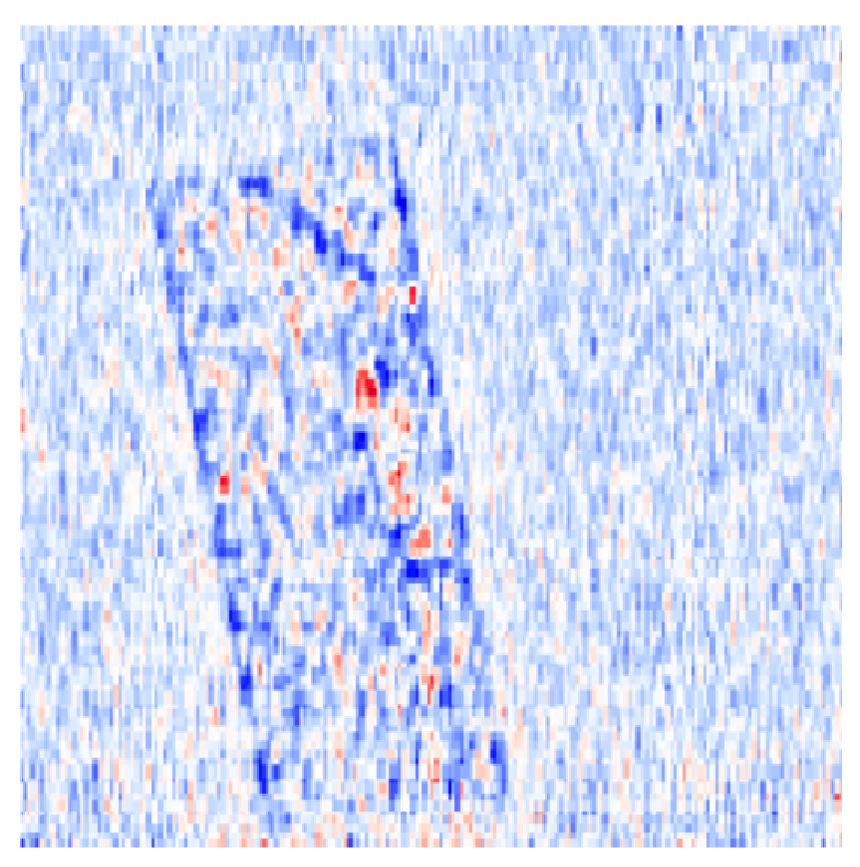
\includegraphics[width=5.7in]{figs/pme_exp/fig3_6_c_lg.ps}
\caption[Magnetization of $30\times 100$ junction array after field
cooling in $\phiext = 1.2$.]{Magnetization of $30\times 100$ 
junction array after field
cooling in $\phiext = 1.2$. The color 
ranges from red, $\phimag = 0.45$ (paramagnetic) 
to blue, $\phimag = -0.45$ (diamagnetic). The long side of the array
is $4.6\,\mathrm{mm}$ long. }
\label{fig:paramag_image_c}
\end{figure}

\begin{figure}[p]
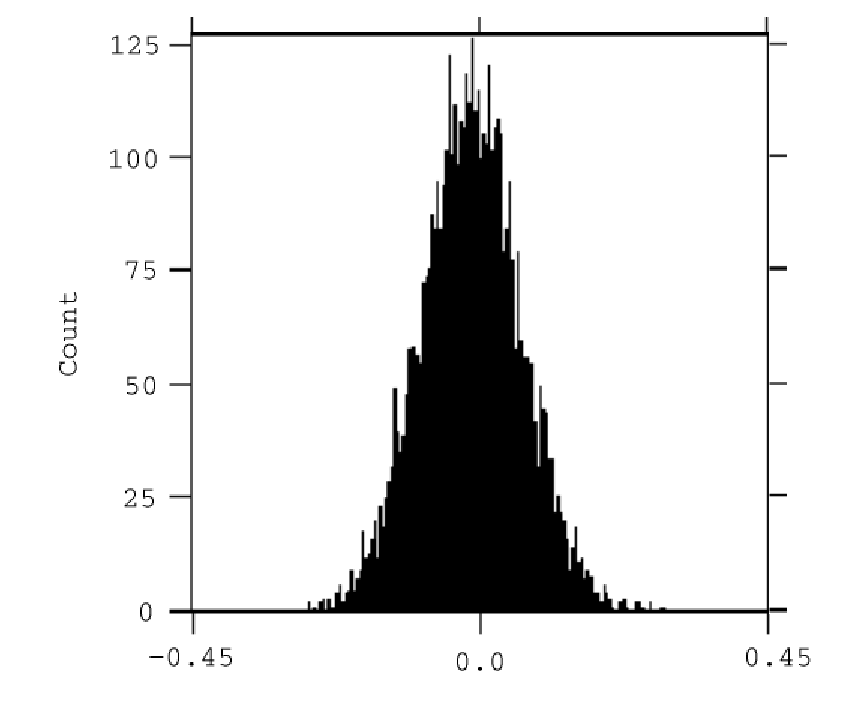
\includegraphics[width=5.7in]{figs/pme_exp/fig3_6_d_lg.ps}
\caption{Histogram of the magnetization data shown
in the magnetization image, \FigRef{fig:paramag_image_c}.}
\label{fig:paramag_image_d}
\end{figure}

If there were no systematic position-dependent errors,
we would need only measure the field-cooled image to 
get \Phitot\ and the image of the field at $13\,\kelvin$ to get \Phiext.
\index{heating}\index{friction}
However,
friction in the plastic scanning mechanism generates heat that  
does not dissipate
quickly into the \lhe\ bath and
warms both the SQUID and the sample by slightly less than $1\,\kelvin$. 
This change in the sample temperature
does not matter. The sample never
warms to the point where thermal activation can overcome the energy
barriers due to the array's Hamiltonian, \EqnRef{eqn:array_hamiltonian}. 
Conversely, the heating of the SQUID is important.
 
\FigRef{fig:squid_vs_temperature} shows how the SQUID output changes 
during a $1\,\kelvin$ temperature change. This change is comparable to the
signal level shown 
in \FigRef{fig:pme_scanning_passes_a}\ through
\FigRef{fig:pme_scanning_passes_d}, so the heating of the SQUID must be
considered in order to validate the results. 
This heating effect depends upon the
sample position because the friction changes during different parts of a
scan. Consequently, each image of the sample will
measure two things, the real flux threading the SQUID \Phitot\
and a false
``flux'' distribution $\Phi_\mathrm{Friction\,@\,4.2\,K}$ 
due to the position-dependent heating.
The false flux distribution will be
different at different temperatures since
the 
sample's 
temperature causes a noticeable heat load
on the SQUID.  

It is further possible that after eliminating the flux from the SQUID
that there might be some background flux impinging upon the sample. 
This is clear in the zero field-cooled image, 
\FigRef{fig:pme_scanning_passes_b}, in which some array response
is evident despite the lack of applied field. This false flux
signal
will be a time-independent $\Phi_\mathrm{background}$ in all the images in
\FigRef{fig:pme_scanning_passes_a}\ through
\FigRef{fig:pme_scanning_passes_d} and will just subtract out. 

The total field-cooled flux in \FigRef{fig:pme_scanning_passes_a}\
thus
contains three sources, the real \Phitot, a false flux reading
in the SQUID due to friction,
and the background flux, so that
%
\begin{equation}
\Phi_\mathrm{FC} = \Phitot + \Phi_\mathrm{Friction\,@\,4.2\,K}
 + \Phi_\mathrm{background}.
\label{eqn:phi_fc}
\end{equation}
%
The total zero field-cooled flux in \FigRef{fig:pme_scanning_passes_b}\ 
also contains a false flux signal due to friction and the background flux
%
\begin{equation}
\Phi_\mathrm{ZFC} =  \Phi_\mathrm{Friction\,@\,4.2\,K}
 + \Phi_\mathrm{background}.
\end{equation}
%
The total measured high-temperature flux in 
\FigRef{fig:pme_scanning_passes_c}\ also contains a false flux due to 
friction. The magnitude 
is different because the SQUID sees a different heat load
due to the higher temperature of the sample,
%
\begin{equation}
\Phi_\mathrm{HT} = \Phiext  + \Phi_\mathrm{Friction\,@\,13\,K}
 + \Phi_\mathrm{background}.
\end{equation}
%
The measured zero-field, high-temperature flux in 
\FigRef{fig:pme_scanning_passes_d}\ is
%
\begin{equation}
\Phi_\mathrm{ZHT} =  \Phi_\mathrm{Friction\,@\,13\,K}
 + \Phi_\mathrm{background}.
\label{eqn:phi_zht}
\end{equation}
%
Eqns.~(\ref{eqn:phi_fc}) - (\ref{eqn:phi_zht}) 
combine to give the total sample magnetization
\begin{equation}
\Phimag = \Phitot - \Phiext = (\Phi_\mathrm{FC} - \Phi_\mathrm{ZFC})-
                              (\Phi_\mathrm{HT} - \Phi_\mathrm{ZHT}).
\label{eqn:mag_correction}
\end{equation}

\FigRef{fig:paramag_image_a}\
shows the magnetization image resulting from the four passes
given in \FigRef{fig:pme_scanning_passes_a}\ through
\FigRef{fig:pme_scanning_passes_d} after applying 
\EqnRef{eqn:mag_correction} to the data. The red colors in the image
represent $M>0$, a paramagnetic magnetization and the blue colors 
represent $M<0$, a diamagnetic magnetization. Qualitatively 
the interior of the array
is more \emph{red} than blue, hence it is paramagnetic. 

For each scan, data are collected every $5\,\micron$ in the $x$ direction
and every $50\,\micron$ in the $y$ direction. The discrepancy between 
data collection in $x$ and $y$ direction results from the scanning
mechanism. The scan lines are in the $x$ direction while the raster
lines are in the $y$ direction. Each image in 
\FigRef{fig:pme_scanning_passes_a}\
through \FigRef{fig:pme_scanning_passes_d}
took approximately 45 minutes to complete. 
Each magnetization measurement must be completed before
the \lhe\ boils out of the Dewar, which has a hold time of 11 to 12 hours.
In order to make several magnetization measurements to check consistency
it would be prohibitive to increase the amount of time required for each
scan. 

\section{Experimental results}

\subsection[$30 \times 100$ junction array]
{$\mathbf{30 \times 100}$ junction array}

We first looked at a $30 \times 100$ \jja\ performing field cooled 
measurements of the type
described above in 
Section \ref{sec:exp_method}. We determined that the array could be 
either paramagnetic or diamagnetic depending upon the cooling field. 
\FigRef{fig:paramag_image_a}\ through
\FigRef{fig:paramag_image_d}\ demonstrates the results of field cooling 
for the array for two external fields, $\phiext = 1.2$ and $\phiext = 4.8$. 
The colors in \FigRef{fig:paramag_image_a}\ and
\FigRef{fig:paramag_image_c}\ represent the magnetization
in the image at each point. 
The colors range from 
red, $\phimag = 0.45$ (paramagnetic data)
to blue, $\phimag = -0.45$ (diamagnetic data).%
\footnote{Recall the definitions made in \EqnRef{eqn:dimensionless_subs}
that $\phi = \Phi/\Phi_0$.}
By looking at the images in \FigRef{fig:paramag_image_a}\
we can qualitatively see that the
array is overall paramagnetic, since it is more red,
although the magnetization
is clearly quite complicated. In \FigRef{fig:paramag_image_c}
the array is overall diamagnetic, since it is more blue. 

There is an additional important feature to note which appears in all of the
magnetization images collected, regardless of the overall array magnetization.
The array always has a diamagnetic screening current (shown in the images
as a blue loop) around the outside
edge, \cf\ \FigRef{fig:paramag_image_a}\  and \FigRef{fig:paramag_image_c}. 

In order to make a quantitative analysis,
we looked at histograms of the individual magnetization images.
For this $30 \times 100$ array, we looked only at the bottom one third
of the array because scratches were accidentally introduced into the 
array \textit{in situ} which produce anomalous results. 
The extent of the
anomalous magnetization due to the scratches matches up well with the 
actual extent of the scratches as observed under the optical microscope.
Because of the close correlation between the location of the scratches
in the magnetic and optical images, it was concluded that the scratches
did not affect the magnetization results very far from the area of the
scratches. 

Histograms for \FigRef{fig:paramag_image_a}\ and \FigRef{fig:paramag_image_c} 
are shown in 
\FigRef{fig:paramag_image_b}\ and \FigRef{fig:paramag_image_d} 
respectively. These two histograms
are representative of the histograms generated for all the data on 
this array. For \FigRef{fig:paramag_image_a}, field cooled
at $\phiext = 4.8$, the mean of \FigRef{fig:paramag_image_b} is 
$\langle\phimag\rangle = 0.068$ with a standard deviation of 
$\sigma = 0.15$,
clearly
greater than zero, so the array is overall paramagnetic. Similarly for
\FigRef{fig:paramag_image_c}, field cooled at $\phiext = 1.2$, 
the mean of \FigRef{fig:paramag_image_d} is 
$\langle\phimag\rangle= -0.016$ with a standard deviation of 
$\sigma = 0.16$,
clearly less than
zero, so the array is overall diamagnetic. 
Interestingly, the histogram data for all of the cooling fields have similar
widths, $\sigma \approx 0.15$. 

%
% fig3.7 - background histograms
%
%\begin{figure}[p]
%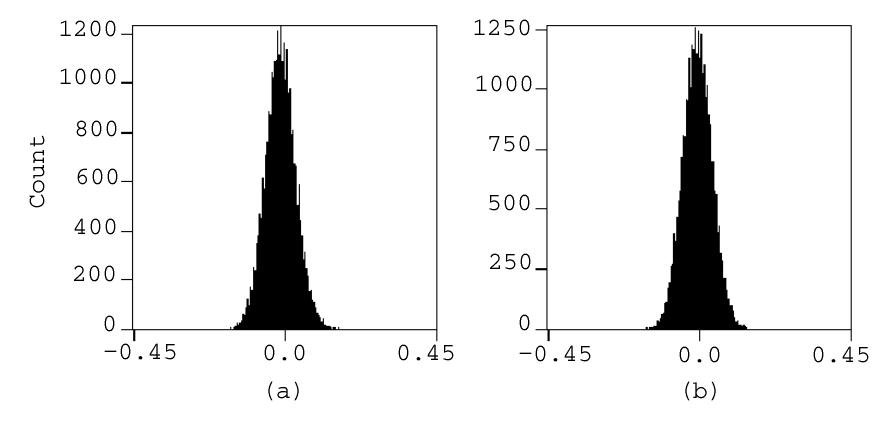
\includegraphics[width=5.7in]{figs/pme_exp/fig3_7.ps}
%\caption[Histograms of the magnetization background.]{Histograms of the 
%magnetization background for the images in \FigRef{fig:paramag_image_a}
%and \FigRef{fig:paramag_image_c}. 
%(a) Histogram of background magnetization for $\phiext = 4.8$. (b)
%Histogram of background magnetization for $\phiext = 1.2$.}
%\label{fig:hist_background}
%\end{figure}

\begin{figure}[p]
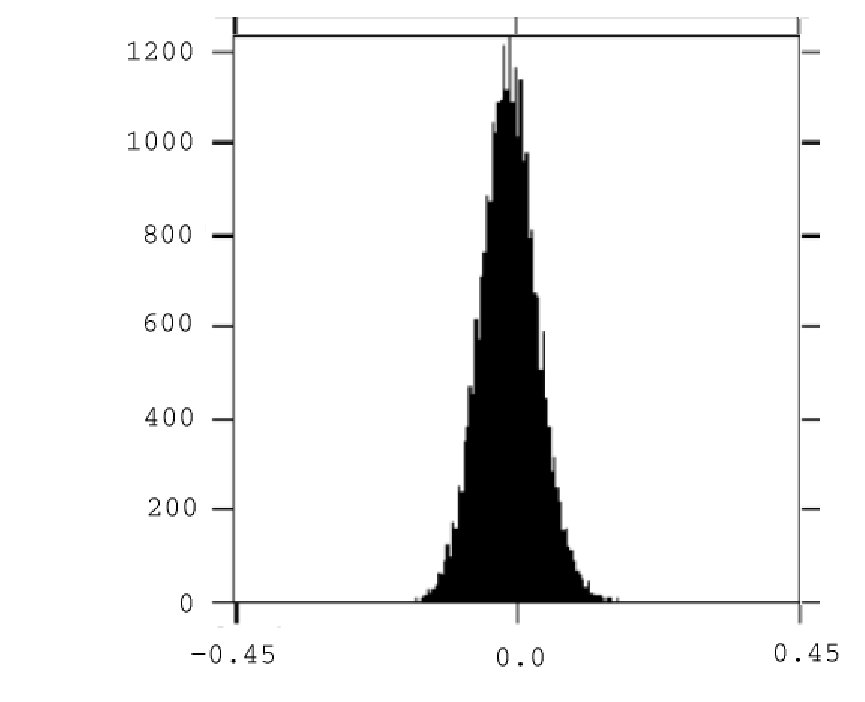
\includegraphics[width=5.7in]{figs/pme_exp/fig3_7_a_lg.ps}
\caption{Histogram of background magnetization for $\phiext = 4.8$, from
\FigRef{fig:paramag_image_a}.}
\label{fig:hist_background_a}
\end{figure}

\begin{figure}[p]
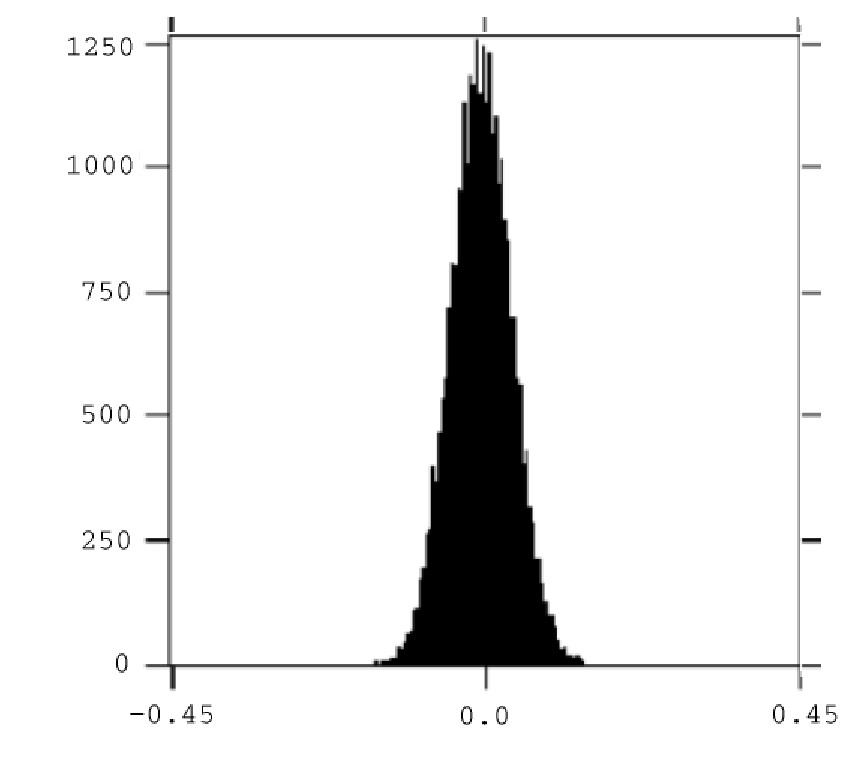
\includegraphics[width=5.7in]{figs/pme_exp/fig3_7_b_lg.ps}
\caption{Histogram of background magnetization for $\phiext = 1.2$, from
\FigRef{fig:paramag_image_c}.}
\label{fig:hist_background_b}
\end{figure}



%
% back ground discussion
%
In each magnetization image, \FigRef{fig:paramag_image_b} and 
\FigRef{fig:paramag_image_d}, a region, 
indicated by a box, was analyzed to 
determine the magnetization of the background. We carried out this
analysis by generating histograms for the background, similar to the
histograms for the array. 
These background histograms are shown 
in \FigRef{fig:hist_background_a} and \FigRef{fig:hist_background_b} 
respectively. 
It is readily apparent from the comparison that the width of the 
background histograms is approximately one-half that of the 
array histograms, and that the mean of the background histograms
is $\langle\phimag\rangle=0.00$ with a standard deviation of
$\sigma = 0.08$, in contrast to the array histograms which
have clear non-zero mean values and $\sigma = 0.15$. 

We have repeated the same types of measurements on this array for 
many different values of the cooling field. These results are 
summarized in \FigRef{fig:sm_array_mag_plot}, which shows the 
measured mean magnetization of the array plotted versus the cooling
field used. Note that the array magnetization is multivalued for some
values of the cooling field. More importantly, although the array may
be diamagnetic for small values of \phiext, it is increasingly
paramagnetic with increasing values of the external field. 
Note that the magnetization curves, as discussed in chapter~\ref{chap:jjarray},
p.~\pageref{jjarray:single_loop_mag}, are very steep for a single loop,
so small variations in \phiext\ may lead to large variations in \phimag\
which could lead to our multivalued solutions. Additionally, we can
see from \EqnRef{eqn:steadystatesolution}\ that a single loop has 
many different solutions for a given \phiext\ so it is not 
unreasonable to think that the array might have multivalued
solutions for a given \phiext\ as well. In fact because the
array is more complicated than a single loop, one might 
expect it to likely be frustrated during field
cooling and to end up in different states for the
same cooling field. 

The range of flux in 
\FigRef{fig:paramag_image_d} (zero field, $T=13\,\kelvin$)
is $0.17\,\Phinot$ per unit cell of the 
array, so we can be confident that the actual gradient of 
the background field is at least this small, meaning that the
array sees flux uniform to $\phiext \pm 0.17$. 
This variation in \phiext\ corresponds to a potential variation
in magnetization of $\pm 0.05$ by comparing with 
\EqnRef{eqn:steadystatesolution}.

Because of the large number of data points that went into computing the 
averages for \FigRef{fig:paramag_image_b} we find
a mean paramagnetic response of $\phimag = 0.063\pm 0.005$.
and for \FigRef{fig:paramag_image_d} we find a mean diamagnetic
response of $\phimag = -0.016 \pm 0.005$. This is a larger
variation than the control we have with the current source to the
solenoid, a Keithley 224 programmable current source
\cite{keithley_instr}.

\begin{figure}[p]
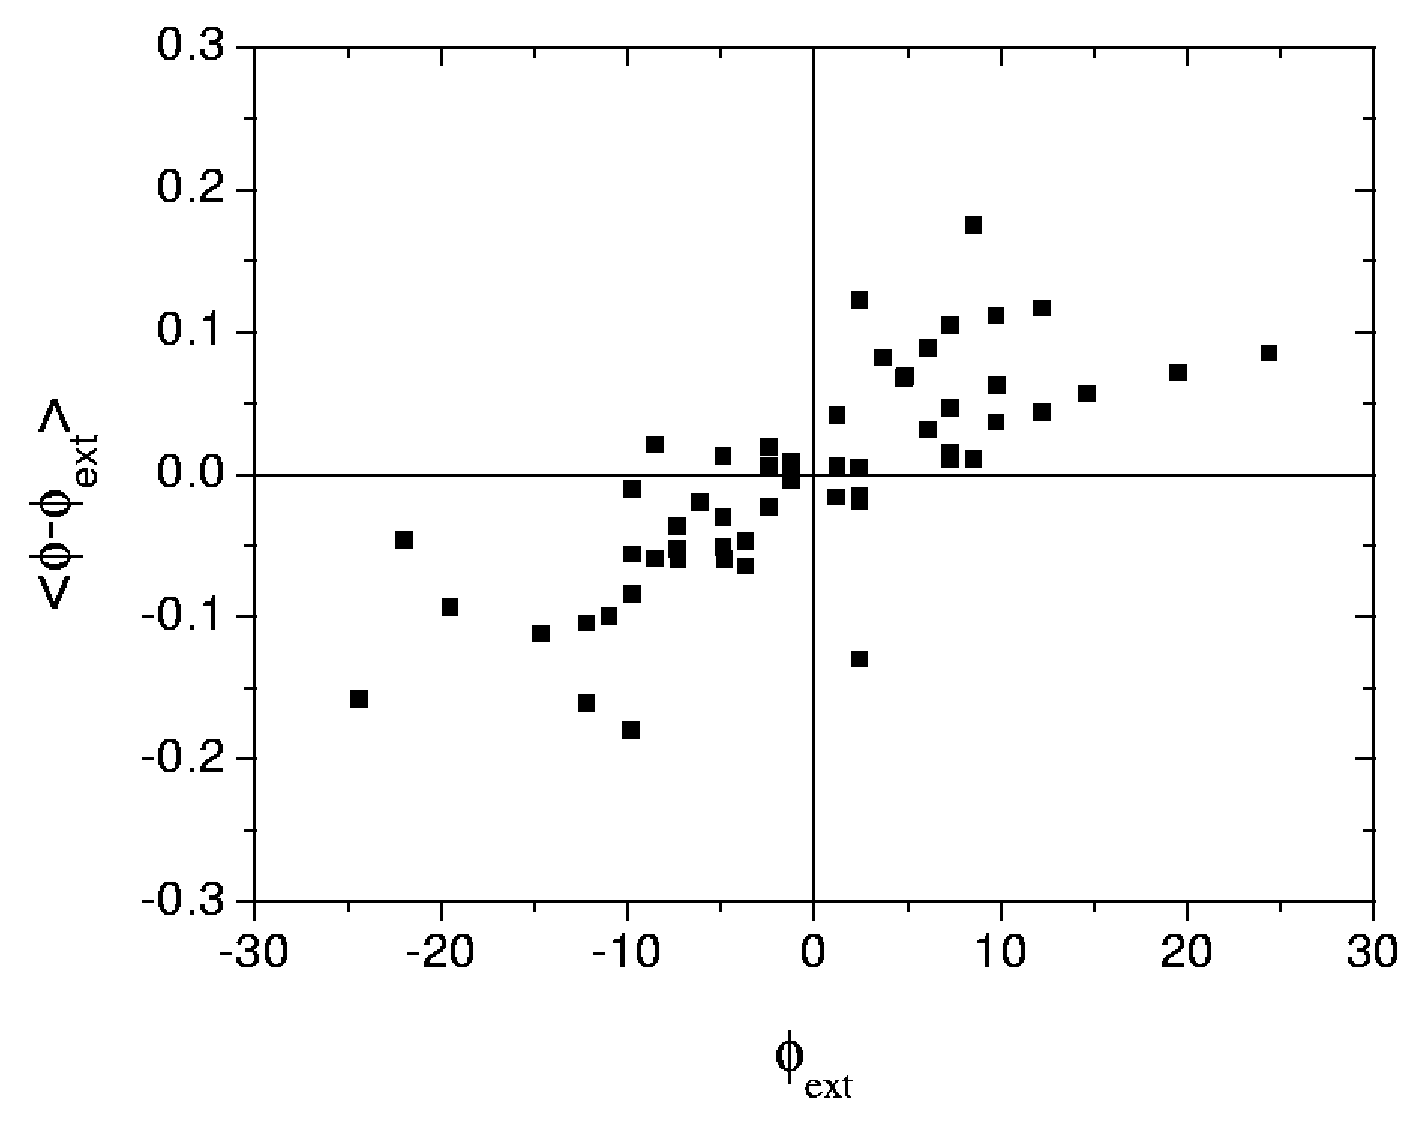
\includegraphics[width=5.7in,keepaspectratio=true]{figs/pme_exp/fig3_8.eps}
\caption[Measured mean magnetization for $30 \times 100$ junction
array plotted versus cooling field.]{Measured mean magnetization
for $30 \times 100$ junction array plotted versus cooling field.
The error in each data point is less than the size of the symbol.}
\label{fig:sm_array_mag_plot}
\end{figure}

\subsection[$100 \times 150$ junction array]
{$\mathbf{100 \times 150}$ junction array}

In addition to the $30 \times 100$ junction array, we were interested
to see 
what effect the geometry of the sample might have upon the measured
magnetization because some theories predict that 
the size of the
sample is important to the paramagnetic response
\cite{geim_nature_396_144_1998,koshelev_prb_53_13559_1995}. 
For this purpose,
we chose to 
look at an array of 
$100 \times 150$ \jjsnoun. This array was otherwise exactly the same as the 
previous $30 \times 100$ junction array and the 
magnetization measurements were
carried out in the same way. 

An 
image showing a paramagnetic state of the larger array is shown
in \FigRef{fig:lg_paramag_image_a} with the corresponding
histogram shown in \FigRef{fig:lg_paramag_image_b}. 
In this data set, for an applied field of $\phiext = -11.0$
the response was paramagnetic, $\phimag = -0.099 \pm 0.005$.
There were
no \insitu\ scratches accidentally introduced into this array, 
however, there was some noise in the SQUID output, present as the
straight horizontal line, in the top of the image,
so we 
were able to analyze the magnetization histogram for the entire array,
except for the noisy region.  

%\begin{figure}[p]
%\includegraphics[width=5.7in]{figs/pme_exp/fig3_9.eps}
%\caption[Paramagnetic image and histogram for $100\times 150$
%junction array.]{Representative paramagnetic image (a) and histogram (b)
%for the $100\times 150$ junction array. The array was field cooled
%in a field of $\phiext = -11.0$. The color scale ranges from blue
%($-0.45\,\Phinot$) to red ($0.20\,\Phinot$) and the short side of
%the array is $4.6\,\mm$ long. 
% }
%\label{fig:lg_paramag_image}
%\end{figure}

\begin{figure}[p]
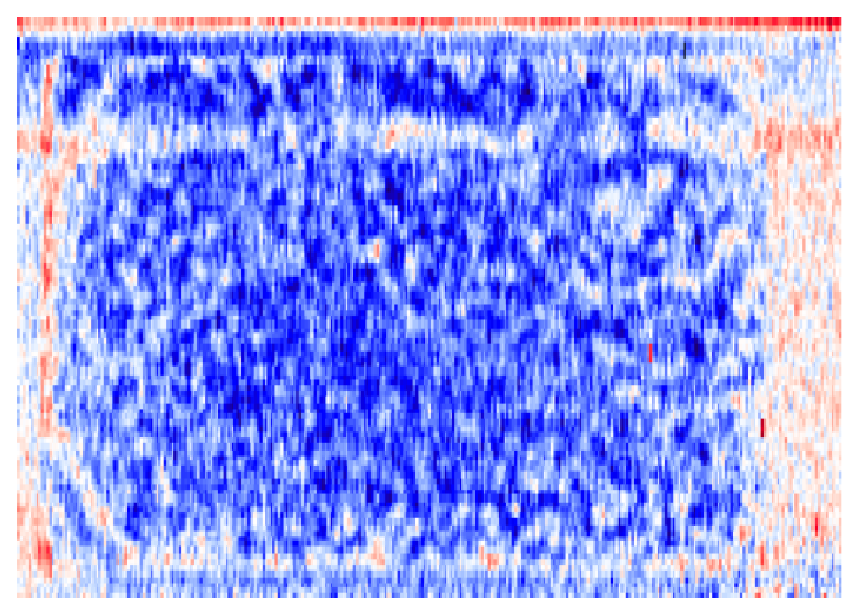
\includegraphics[width=5.7in]{figs/pme_exp/fig3_9_a_lg.ps}
\caption[Representative paramagnetic image
for the $100\times 150$ junction array.]{Representative paramagnetic image
for the $100\times 150$ junction array. The array was field cooled
in a field of $\phiext = -11.0$. The color scale ranges from blue
($-0.45\,\Phinot$) to red ($0.20\,\Phinot$) and the short side of
the array is $4.6\,\mm$ long. }
\label{fig:lg_paramag_image_a}
\end{figure}

\begin{figure}[p]
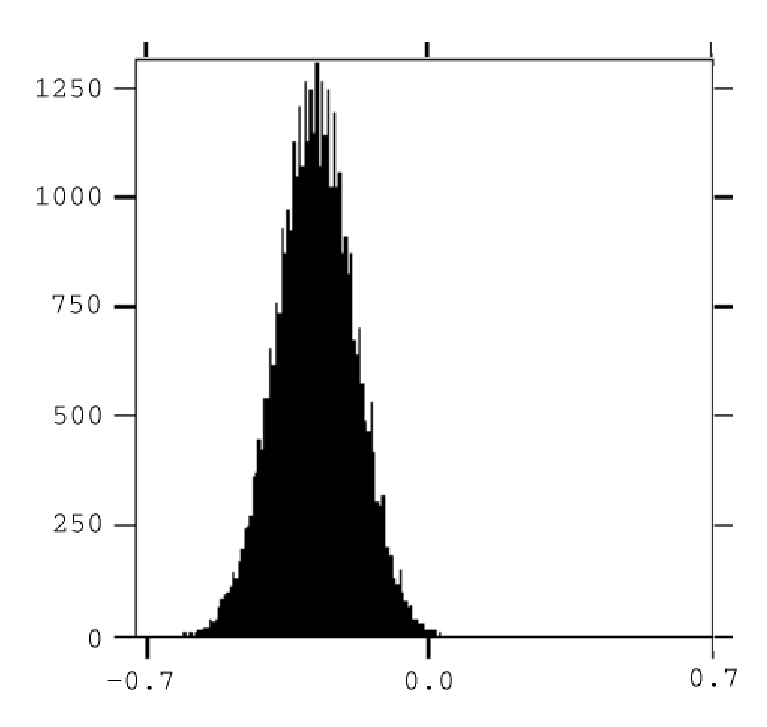
\includegraphics[width=5.7in]{figs/pme_exp/fig3_9_b_lg.ps}
\caption[Paramagnetic histogram shown in \FigRef{fig:lg_paramag_image_a}.]
{Paramagnetic histogram shown in \FigRef{fig:lg_paramag_image_a}.
The array was field cooled
in a field of $\phiext = -11.0$. The color scale ranges from blue
($-0.45\,\Phinot$) to red ($0.20\,\Phinot$) and the short side of
the array is $4.6\,\mm$ long. }
\label{fig:lg_paramag_image_b}
\end{figure}



The results from this measurement compare favorably with the results
made on the smaller array. In \FigRef{fig:lg_mag_vs_ext}\ the 
large array mean magnetization is plotted against the cooling field. 
In agreement with the previous results on the smaller array, we see that
the array magnetization increases with increasing external field.
The magnitude of the magnetization is comparable. Additionally,
as is evident in \FigRef{fig:lg_paramag_image_a} the array, to which
an external field of $\phiext=-11$ has been applied,  has a
diamagnetic screening current (colored red in this figure) 
around the outside. This diamagnetic screening
current is again visible in all the images of the large array. 

\begin{figure}[p]
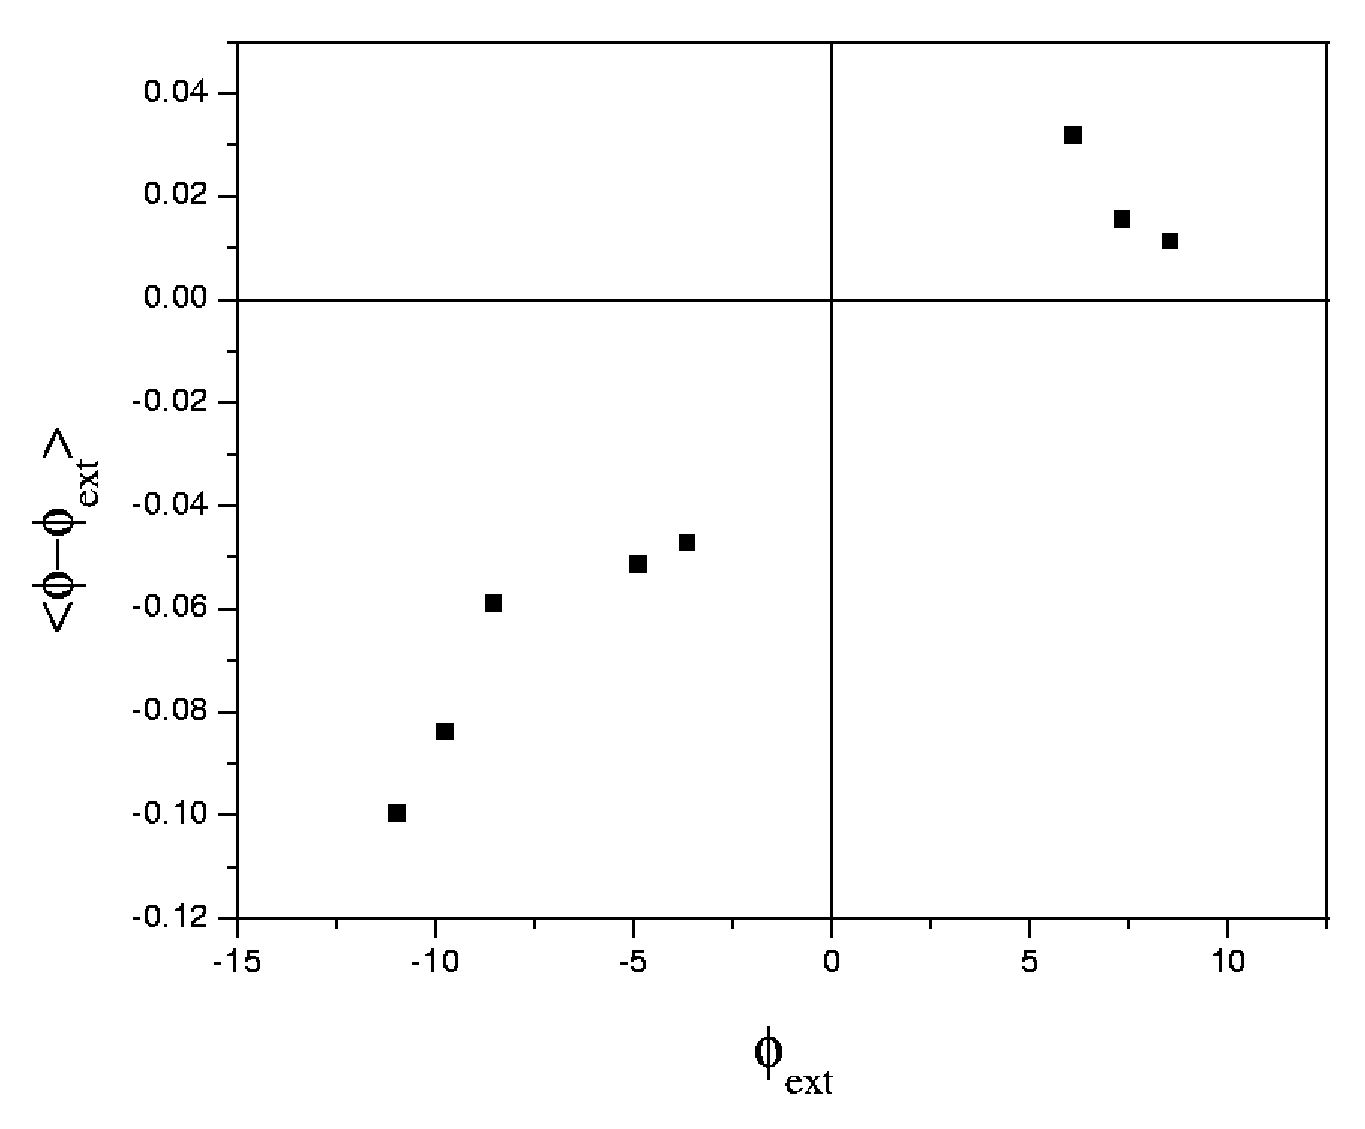
\includegraphics[width=5.7in]{figs/pme_exp/fig3_10.eps}
\caption[Measured mean magnetization versus cooling field for
$100 \times 150$ junction array.]{Measured mean magnetization versus
cooling field for the $100 \times 150$ \jja. The error for each 
data point is smaller than the size of the symbol.}
\label{fig:lg_mag_vs_ext}
\end{figure}

\section{Summary of magnetization measurements}

Arrays of $30 \times 100$ and $100\times 150$ junctions were
measured in field-cooling experiments using a scanning SQUID microscope. 
The results on the arrays are very similar, both in magnitude of 
array magnetization and in average 
magnetization dependence upon external field. 
The next chapter will explain the various phenomena observed
here and reconcile them with the ideas presented in 
chapter \ref{chap:jjarray}. 

In both cases the array magnetization increases with increasing external
field, and the array is preferentially paramagnetic. This is in contrast
to the single-loop model which predicts equally that the the single loop
will be either paramagnetic or diamagnetic equally often.  

The magnetization internal to the array takes on a somewhat complicated,
randomly distributed arrangement. The magnetization
at the edge is always diamagnetic, regardless of the internal magnetization. 

 


\chapter{A model of PME in multiply-connected superconductors}
\label{chap:pme_theory}

\section{Introduction}

As discussed in the chapter \ref{chap:pme_experiment}, there have 
been many previous observations of PME in superconductors. 
In addition to these experimental observations, there 
have also been several attempts to describe a model for 
the PME in these superconductors. 

\subsection{\pijunction\ models}

The first attempt to describe PME in \hightc\ came from
Sigrist and Rice \cite{sigrist_jpsj_61_4283_1992,%
sigrist_rmp_503_67_1995}\ who argued that the presence 
of \pijunctions in a superconductor would cause it to be
paramagnetic. They further argued that \pijunction s would
come about due to a \dwave\ order parameter coupled with
misaligned grains in the superconductor. This idea is basically
the single loop model as discussed in chapter \ref{chap:jjarray}
(section \ref{sec:single_loop}, p. \pageref{sec:single_loop}, 
\EqnRef{eqn:steadystatepijunction}).
It was discussed that Sigrist and Rice chose a value of 
\betal\ that was too small. Had they chosen a larger value
of \betal\ they would have seen that paramagnetism would be 
possible at $\phiext=0$, for a loop with no \pijunctions\, 
a phenomena which they attributed
to the presence of a \pijunction\ in the loop. It should be noted
that Sigrist and Rice proposed this theory before the first
observation of PME in \lowtc\ superconductors\cite{thompson_prl_75_529_1995}.

Because the Sigrist and Rice work was based on the idea of a 
single superconducting loop, others began to try and model the
superconductor as various types of \jjas. One model
was carried out by Dominguez \etal\cite{dominguez_prl_72_2773_1994}
but contained several flaws. They treat the case of a \jja\ with 
randomly distributed \pijunctions, but do not treat they case of an
array without \pijunctions. This failing is similar to that of 
Sigrist and Rice, and they reach the similar conclusion that 
the presence of \pijunctions\ make the sample behave 
paramagnetically. 

\subsection{\jja\ models}

Similar models of this
type were carried out by Auletta \etal\cite{auletta_prb_49_12311_1994}
who modeled the array as a series of concentric loops of \jjsnoun\  
with mutual
inductance. Additionally, Chandran\cite{chandran_prb_56_6169_1997}
performed similar calculations using a square array and a full
mutual inductance matrix. 
Both Auletta \etal\ and Chandran use 
simplified models for the \jjsnoun\
which ignore the capacitance of the
junction (RSJ model). 
Additionally, both treat only the case of no \pijunctions, 
alleviating the problems with the Sigrist and Rice and the Dominguez \etal\
models. 
Remarkably, however, they are able to recreate the 
temperature dependent magnetization during a field cooling experiment. 
Unfortunately, neither report on the spatial distribution of the
magnetization over the array, which is what we have measured directly
here. 

More recently, De Leo \etal\cite{deleo_unpublished}, modeled 
an RCSJ \jja\ dynamically through the field-cooling process, and 
obtained results remarkably similar to those discussed in 
chapter \ref{chap:pme_experiment}. The relationship between this model
and the experiment will be discussed in more detail in section
\ref{sec:num_array_sims}. 

\subsection{Flux compression}

In a departure from the \jja\ model of PME there have been other
proposed models. Koshelev and Larkin\cite{koshelev_prb_53_13559_1995}
proposed the so-called flux compression model. \index{flux compression}
The flux compression model relies on the superconductor having a 
spatial variation in $T_c$, such that the exterior of the sample
becomes superconducting before the interior of the sample, through
either a differential cooling or a spatial distribution of 
$T_c$. Because the exterior becomes superconducting first, it 
effectively traps flux in the center of the sample, and compresses
the trapped flux (hence ``flux compression'') as the 
superconducting region grows
from the outside-in. This trapped flux, and the
screening currents required to keep the flux trapped, create
a positive magnetic moment, the paramagnetic Meissner effect.
An interesting aspect of the flux compression model is that it gives
specific predictions for the flux and current distribution
throughout the sample -- something that can easily be tested with
the SQUID microscope. 

A phenomena related to the flux compression model is the ``giant
vortex state'' model\cite{moshchalkov_prb_55_11793_1999,%
deo_prl_79_4653_1997} which is appropriate for mesoscopic
superconductors, such as the Al disks measured by Geim \etal\
\cite{geim_nature_396_144_1998}, but does not apply to the 
macroscopic situations discussed here. 

\subsection{Pinning and surface barriers}

In addition there are other proposed models which essentially rely
on defects in the superconductor to create the PME. 
One may imagine, \eg\, that surface damage to the superconductor
pins flux during the field cooling process 
and causes the sample to be paramagnetic. It has
additionally been proposed that some type of surface barrier
may result in flux trapping in the sample\cite{deo_prb_59_6039_1999},
or that 
Andreev bound states at the
surface of the superconductor\cite{prusseit_physc_317_396_1999}
may result in paramagnetism. 

\section{Experimental comparison to various models}

It has already been stated that the simple models involving \pijunctions\
do not reflect reality in the \jja\ samples that were measured. 
It has clearly been demonstrated that Nb, an \swave\ superconductor,
exhibits PME in the absence of \pijunctions. Furthermore, it is
clear from the discussion of the single loop in chapter \ref{chap:jjarray}\
that a single loop of \jjsnoun, without any \pijunctions, can in
theory be paramagnetic after field cooling. 

The various models treating PME in an array model of superconductivity
have great merit, but do not provide any spatially resolved data
to which we might compare our array data.

Based on our experimental observations we can clearly rule out
the flux compression model as untenable. Our data looks nothing
like the proposed flux distribution for a sample exhibiting
flux compression. Furthermore, we do not expect any of the 
requirements of flux compression to be met in our experiment. 
Our sample is well grounded thermally to the sapphire rod of the
sample stage in the experiment. Furthermore because of the
photolithographic uniformity
we do not expect that the outermost islands of the 
array would have a $T_c$ \emph{higher} than the inner islands. 
If anything we would expect deposition errors to cause the edge 
islands to have defects
which would tend to 
\emph{lower} the $T_c$. 

Indeed, the primary features of our experimental data are not
predicted by any of the known theories of PME. We always observe a
diamagnetic region around the edge of the sample in addition to 
a region of Gaussian distributed flux inside, but generally with
a  paramagnetic mean. Finally the paramagnetism of the array increases
with increasing external field. 

\section{Array screening}

The presence of the diamagnetic screening current flowing around
the outside edge of the array must be accounted for in any 
realistic model. The array could possibly accomplish this diamagnetic
screening in one of two ways. 

\begin{figure}
\includegraphics[width=5.0in]{figs/pme_theory/fig41.eps}
\caption[Comparative array screening: individual plaquette \vs\ 
large outside loop]
{Comparative ways to generate Meissner screening in an array.
(a) A large loop of many \jjsnoun\ around the outside edge of the
array. (b) Each plaquette single screening flux from the interior
of itself, and hence screening from the entire array. }
\label{fig:comp_array_screening}
\end{figure}

First, the array may generate a screening
current flowing around the outside edge of the array; in effect
creating a large loop of $2(N + M)$ junctions around the outside
of the array. 
\MultFigRef{fig:comp_array_screening}{a}\ depicts this situation. 
This picture is similar to how a bulk 
superconductor might screen, with current flowing just around the outside
edge and nowhere else inside. 
We can quickly see that this
large loop can screen a maximum external field of 
$B_{\mathrm{max}}=\Phinot \betal /2 \pi a^2 (NM)^{1/2}$. This
maximum field shrinks as the size of the array, $NM$, increases.

The second possibility, depicted in 
\MultFigRef{fig:comp_array_screening}{b}\ is that each plaquette 
may screen flux from 
itself. In this case, each plaquette may screen up to 
$B_{\mathrm{max}} = \Phinot \betal /2 \pi a^2$. 
In this picture, flux will not penetrate the array until flux
is able to penetrate a single plaquette. The maximum
field in this case is always greater, and substantially greater
for large arrays, than for the single loop, making this difference
quite easy to discern experimentally. 

One clear way to think about these two configurations is to realize 
that in both cases, the maximum current that may flow around any 
current path is $I_c$. Presented here are the two limiting cases. 
In the large loop current case, the maximum field is screened with
$I_c$ flows around the entire array. In the second case, the maximum
flux may be screened when $I_c$ flows around a single plaquette. 
It is clear that the amount of flux that flows through the enclosed
area, due to the currents, is far larger in the latter case than
in the former. 

Indeed, 
AC susceptibility measurements by Araujo-Moreira \etal
\cite{araujo_prl_78_4625_1997} demonstrated this, in arrays of the 
same geometry as those discussed here. They showed that 
the array did not respond hysteretically to a driving external field
until the amplitude of the external field was increased above approximately
$4\,\Phinot$ per unit cell. For the $\betal =30 $ used here this
indicates that single
plaquettes of the array are screening.  

Furthermore, we have observed flux penetration into our array in the
Meissner state and noticed that the flux does not penetrate until the
external field is ramped from zero to exceed $4\,\Phinot$ per unit cell
of the array. An example of this penetration is shown in 
\FigRef{fig:init_flux_penetration}. The figure shows the first
flux penetration into the array at a field of $4.8\,\Phinot$ per unit cell 
of the array. Notice that the flux penetrates as fingers, apparently
nucleating from a single plaquette, indicating that it was the screening
of a single plaquette that broke down (perhaps due to a weak $J_c$) 
and allowed flux to penetrate. 

\begin{figure}
\includegraphics[clip=true]{figs/pme_theory/fig42.eps}
\caption[Initial flux penetration into \jja]{Initial flux 
penetration into \jja\ at an external field of 4.8 \Phinot.}
\label{fig:init_flux_penetration}
\end{figure}

\subsection{Outer diamagnetic current}

The previous section demonstrated that the each plaquette of the array
screens flux from itself, rather than the entire array 
screening by way of a large current loop around the outside edge
of the array. 
However, it was observed 
(\cf\ \FigRef{fig:paramag_image}(a) and (c) ) in all of the 
cooling images that the array always generated a diamagnetic 
screening current around the outside edge. To
generate an overall diamagnetic screening current,
and have each plaquette screening individually, one may think
that they array constructs a picture as in 
\MultFigRef{fig:plaquette_screening}{a}, in which all the 
internal currents of the array cancel to generate an overall
diamagnetic current. 

\begin{figure}
\includegraphics[width=5.0in]{figs/pme_theory/fig43.eps}
\caption[Different array screening configurations for individual
plaquettes]
{Possible different array screening configurations. (a) Every
plaquette of the array screening. (b) Only the outside edge plaquettes
of the array screening. }
\label{fig:plaquette_screening}
\end{figure}

However, it may not be true that the currents cancel. For our array
geometry, the array wire width is $10\,\micron$, but the penetration
depth of niobium at $4.2\,\kelvin$ is $900\,\angstrom$. This means that
the internal currents of the array will not cancel. Instead currents
flow internal to the array around each plaquette. 
\FigRef{fig:plaquette_screening_close_up} schematically demonstrates
this situation for two neighboring plaquettes. 
Because of the discrepancy between the wire width
and the penetration depth of niobium, the internal currents do not
cancel. Instead each screening loop of the array must generate 
a current flowing around the plaquette. 

\begin{figure}
\includegraphics[width=5.0in]{figs/pme_theory/fig44.eps}
\caption[Close up view to two adjacent screening plaquettes]
{Close up view of two adjacent screening plaquettes. The geometry
is for our array. The wire width is $10\,\micron$ and the penetration
depth for niobium is $900\,\angstrom$. Because of this discrepancy,
the internal currents do not cancel, as shown, and the array
must actually generate a loop of current flowing around each
plaquette}
\label{fig:plaquette_screening_close_up}
\end{figure}

% currents canceling in overlap geometry junctions. 
It is argued above that 
the internal currents to the array do not cancel within the wires. 
It turns out that in the overlap \jjnoun\ geometry the current
flowing through the \jjnoun\ spreads out uniformly so we expect
the currents flowing through the junctions to cancel, and not
give a contribution to the net Josephson energy. 

To generate this configuration we find that the energy stored
magnetically due to all the plaquette current loops in the array 
is
%
\begin{equation}
E_{\mathrm{mag}} = NM\, \frac{1}{2} LI^2.
\end{equation}
%
Additionally, there is a Josephson energy contribution to the energy
from the junctions around the outside edge of the array
%
\begin{equation}
E_J = 2(M+N)\, E_J (1-\cos\gamma)
\end{equation}
%
This leads to a total energy of 
%
\begin{equation}
E_{\mathrm{tot}} =  NM \,\frac{1}{2} LI^2 + 
          2(M+N)\, E_J (1-cos\gamma).
\label{eqn:all_loop_screening}
\end{equation}
%
This total energy grows as $N\times M$, and for a large array can be quite 
substantial. 

It turns out that it is possible to create a screening mechanism, in
which the total array energy grows as $N+M$. 
This screening configuration is shown in 
\MultFigRef{fig:plaquette_screening}{b}. Here only the plaquettes on 
the outside edge of the array screen. This creates the observed external
diamagnetic screening current. But we end up with a total magnetic
energy of 
%
\begin{equation}
E_{\mathrm{mag}} = 2(N+M)\, \frac{1}{2} LI^2.
\end{equation}
% 
Additionally, there is a contribution due to the Josephson energy
in the outside edge junctions, but also due to the edge 
junctions just inside the screening plaquettes, as shown in 
\MultFigRef{fig:plaquette_screening}{b}. 

in the inside edge junctions
%
\begin{equation}
E_J =\left\{ 2(N+M) + 2(N + M - 2) \right\}\, E_J (1-\cos\gamma),
\end{equation}
%
yielding a total energy of 
%
\begin{equation}
E_{\mathrm{tot}} = 2(N+M)\, \frac{1}{2} LI^2 +
 \left\{ 2(N+M) + 2(N + M - 2) \right\}\, E_J (1-\cos\gamma).
\label{eqn:edge_loop_screening}
\end{equation}
%
This energy is smaller than the energy in the previous case
in which all of the plaquettes screen. As the size of the array
grows, this energy becomes more favorable (\cf\ $N+M$ \vs\ $N\times M$).

Comparing \EqnRef{eqn:all_loop_screening}\ and 
\EqnRef{eqn:edge_loop_screening}\ and assuming that $\gamma$ is 
proportional to $\Phitot$ and $N=M$
we deduce that it will be energetically
favorable for the array to screen with only the outside when,
%
\begin{equation}
\betal > {4 N -1 \over N^2 - 4N}
\end{equation}
%
which is valid for all $N>2$. For the arrays we consider, this 
criteria is easily satisfied. 

\section{Consequences of edge loop screening}

In the second case, with only the edge loops screening, 
in addition to the diamagnetic screening current flowing immediately
around the outside edge, there also is a paramagnetic
current flowing just inside the outside edge. This paramagnetic
current is closer to the interior of the array than the diamagnetic
current. The interior plaquettes of the array will respond to both
the diamagnetic current and the paramagnetic current, but the 
paramagnetic current is closer to the interior plaquettes, so 
it will dominate the response of the interior plaquettes. 
\FigRef{fig:screening_schematic}\  schematically shows this situation, 
depicting the external diamagnetic screening current and the interior
paramagnetic current.

\begin{figure}
\includegraphics[width=5.0in]{figs/pme_theory/fig45.eps}
\caption[Schematic of interior and exterior plaquettes, with screening
provided by external plaquettes only]
{Schematic of interior and exterior plaquettes, with screening provided
by external plaquettes only. The diamagnetic screening current flows 
around the outside edge of the array, while the paramagnetic current
flows just inside the edge of the array.}
\label{fig:screening_schematic}
\end{figure}

\subsection{Single loop response to external field shift}

Each interior plaquette essentially sees a shift in the external field
applied to it, due to the diamagnetic and paramagnetic currents
discussed above. 
We must consider the effect of these two currents to the 
single loop's magnetization before continuing. The external flux
that each interior plaquette sees is the real external flux, 
plus a contribution due to the external currents
%
\begin{equation}
\Phiext -> \Phiext + \Phi_{\mathrm{screen}}.
\label{eqn:ext_flux_redef}
\end{equation}
%
If we apply this modification to the magnetization relation for a 
single loop, shown in \FigRef{fig:single_loop_mag}, we see that the
entire magnetization curve for the single loop is shifted upward
so that the single loop will more often appear to be 
\emph{paramagnetic}. It must be pointed out here that this 
shift is really just a book-keeping shift, because of the 
redefinition of the external flux that affects the single 
loop, \EqnRef{eqn:ext_flux_redef}. 

\subsection{Array response to external shift}

We computed the $\Phi_{\mathrm{screen}}$ term
over the entire interior of the array
for the geometry of the $30 \times 100$ array;
determined the shift in the magnetization of each interior
plaquette; and found that the 
minimum induced magnetization occurs in the central plaquette of
the array and is approximately $\Phimag=0.15\,\Phinot$. Furthermore,
we can determine the average induced magnetization over the 
entire interior of the array, and determine it to be 
$\Phimag=0.27\,\Phinot$. These numbers compare favorably with the observed
average
magnetization numbers seen in the array (\cf\ \FigRef{fig:sm_array_mag_plot}).

Of course, this simple model does not capture many other important
features experimentally observed in the array. It does not explain
\eg\ the apparent random distribution of flux over the interior of the
array. Quite the contrary, it predicts that the paramagnetism should
be strongest near the edges of the array, and weakest in the center
of the array. Furthermore, this simple model predicts that they array
interior
should be entirely paramagnetic while it we observe that there
are diamagnetic regions in the array interior. 

\subsection{Numerical array simulations}
\label{sec:num_array_sims}

Fortunately, numerical simulations of an array system similar to ours,
using the RCSJ model for the entire array (\cf\ chapter \ref{chap:jjarray},
section \ref{sec:entire_array_model}, p. \pageref{sec:entire_array_model}
and  Eqns.~(\ref{eqn:junc_horiz}) to 
(\ref{eqn:total_flux_array})) have been carried out recently%
\cite{deleo_unpublished} and obtain results that replicate quite
well the experimentally observed flux distribution in the array.

In this numerical experiment, De Leo \etal\ take a $10\times 40$ 
\jja\ and model the experiment by increasing \betal\
and \betac\ from zero to their final values at $T=4.2\,\kelvin$
to simulate the field cooling process. After waiting for
transient solutions to decay, a steady state solution is arrived 
at for the array. 

\begin{figure}
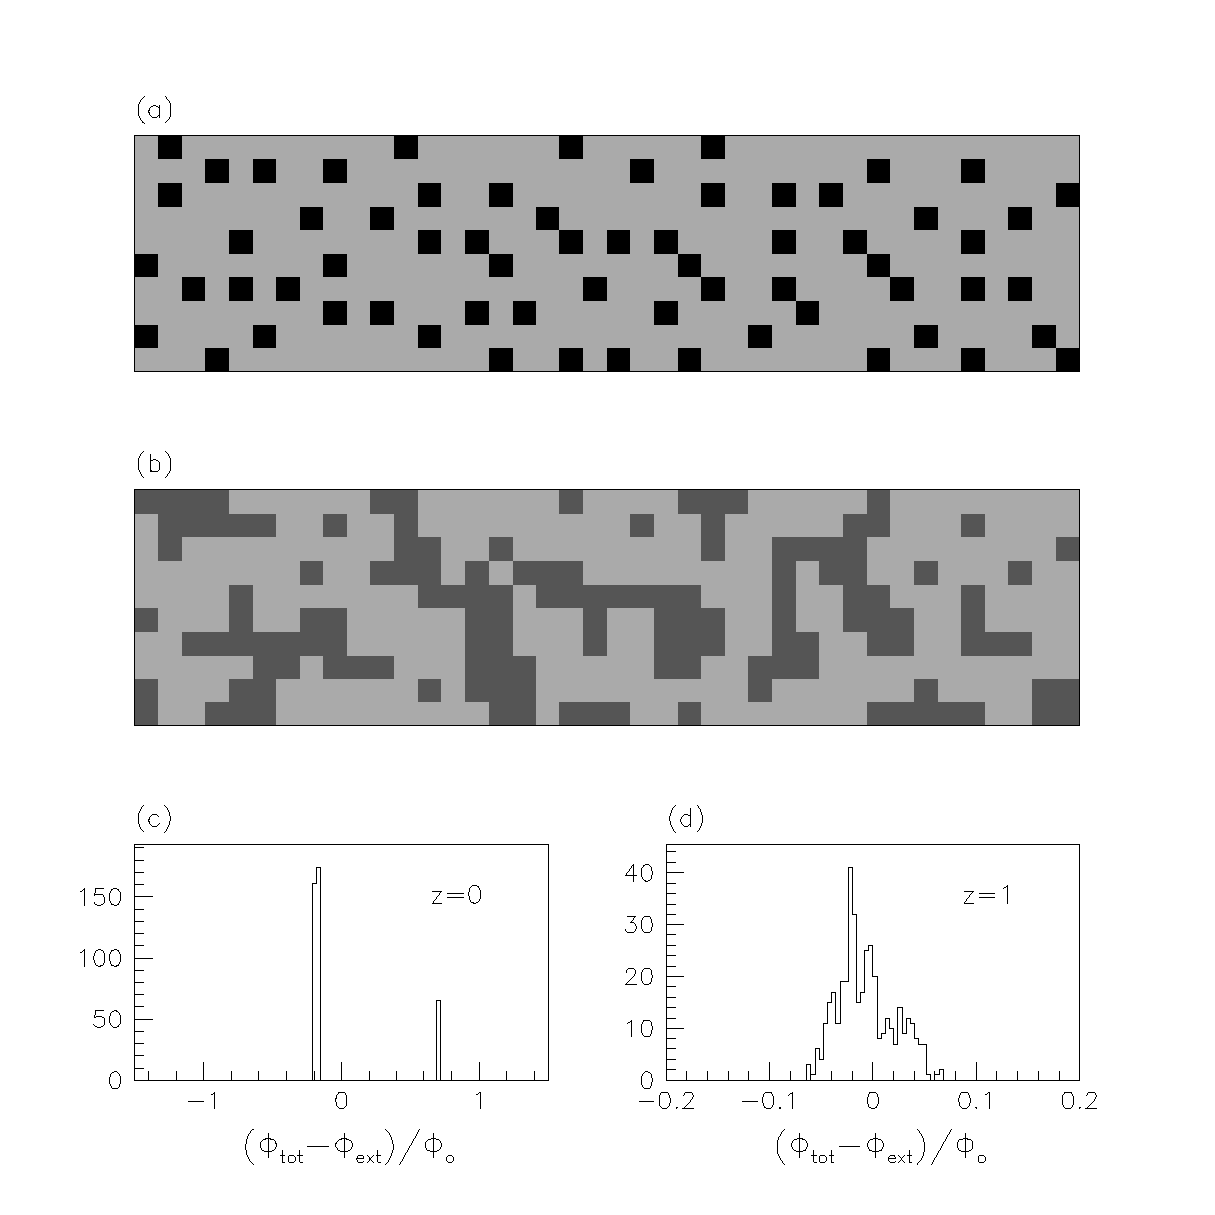
\includegraphics[width=5.0in]{figs/pme_theory/fig46.eps}
\caption[Modeled array magnetization for a $10\times 40$ \jja,
field cooled in $\phiext = 4.8$]
{Modeled array magnetization for a $10\times 40$ \jja, field
cooled in $\phiext = 4.8$. 
Red represents paramagnetic plaquettes and blue represents
diamagnetic plaquettes.
(a) The array magnetization at the surface of the array. 
(b) The array magnetization as measured at a height of one
unit cell above the array. 
(c) Histogram of the array magnetization at the surface of the
array.
(d) Histogram of the array magnetization at a height of one
unit cell above the array. }
\label{fig:model_array_mag}
\end{figure}

\FigRef{fig:model_array_mag}\ shows the results of the field
cooling simulation for a $10 \times 40 $ \jja. Red colors represent
paramagnetic plaquettes and blue colors represent diamagnetic 
plaquettes. \MultFigRef{fig:model_array_mag}{a}\ shows the 
magnetization as measured at the surface of the array, and
\MultFigRef{fig:model_array_mag}{c}\ shows a histogram of the
same data. The spatial distribution of the magnetization in (a)
is very suggestive of the data as we measured (\cf\ 
\FigRef{fig:paramag_image}). However, the histogram in 
\MultFigRef{fig:model_array_mag}{c} is quite different from that
measured in \MultFigRef{fig:paramag_image}{b}. What's truly
striking about  \MultFigRef{fig:paramag_image}{b}\ however, is that
the two peaks correspond almost exactly to the lowest and second
lowest Gibbs free energy solutions for the single loop
(\cf\ chapter \ref{chap:jjarray}, section \ref{sec:gibbs_free_energy},
p. \pageref{sec:gibbs_free_energy}). Perhaps more interesting is
\MultFigRef{fig:model_array_mag}{b}\ which shows the simulated
magnetization of the $10 \times 40 $ array at a height of one 
plaquette. This is similar to the magnetization that a SQUID might
measure at a height of one plaquette. Indeed the SQUID in our 
experiments was at a height of approximately one plaquette. 
Interestingly, the histogram shown in \MultFigRef{fig:model_array_mag}{d}\
closely resembles the experimental histogram in 
\MultFigRef{fig:paramag_image}{d}.

Furthermore, De Leo \etal\ modeled the external field dependence of the 
array magnetization, shown in \FigRef{fig:sim_array_mag}. Their results
qualitatively resemble the results obtained in \FigRef{fig:sm_array_mag_plot}\
providing good evidence that the properties of our array can be replicated
simply from the equations describing a \jja. 

\begin{figure}
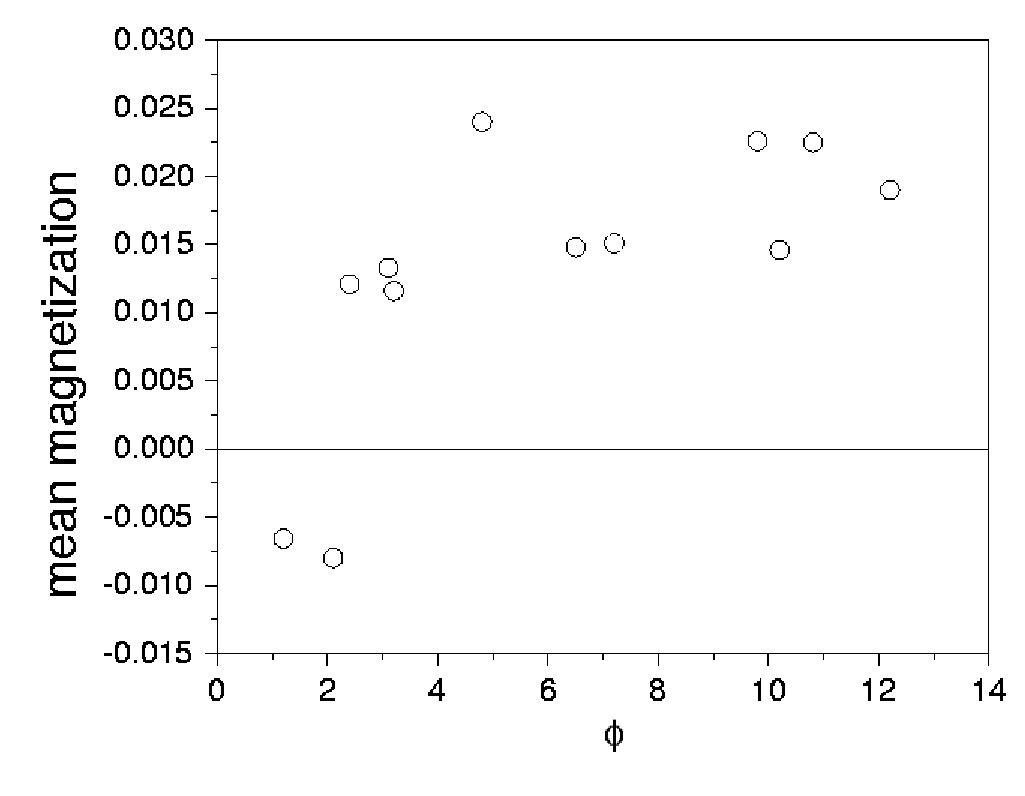
\includegraphics[width=5.0in]{figs/pme_theory/fig47.eps}
\caption[Simulated array magnetization \vs\ cooling field]
{Simulated array magnetization \vs\ cooling field for the 
$10\times 40 $ \jja.}
\label{fig:sim_array_mag}
\end{figure}


% magpen.tex
%
% originally based on magpen1.tex -- first draft of paper on magnetic
% penetration
%
% modified to include some discussion of RABITS as well as the
% YBCO/STO sample discussed in the paper. 

% 29 May 2001 with comments from Chris
% 30 May 2001 with comments from Fred
% 30 May 2001 comments from Paola
% 30 May 2001 comments from R. Gomez

\chapter{Magnetic penetration into $\ybcoheading$ thin films}
\label{chap:magpen}




%\author{A. P. Nielsen and C. J. Lobb}
%\address{Center for Superconductivity Research,
%         Department of Physics \\
%         University of Maryland, College Park, MD 20742, USA}
%
%\author{Paola Barbara}
%\address{Department of Physics, Georgetown University, Washington DC 20057}
%
%\author{H. R. Kerchner}
%\address{Oak Ridge National Lab, Oak Ridge, TN}

%
% abstract from magpen1.tex paper
%
%We have measured, using a scanning SQUID microscope, 
%the magnetic penetration into 
%a thin ($1\,\micron$)
%superconducting 
%$\ybco$ film (of $3\,\mathrm{mm} \times 15\,\mathrm{mm}$ geometry), 
%with the field applied perpendicular to the thickness. 
%We observe the Meissner state and find the onset of flux penetration into the 
%superconductor to occur at a field less than $300\,\mOe$. Additionally,
%we infer the current distribution in the Meissner state and demonstrate that 
%it agrees with well known theoretical results. We further observed 
%the remanence, after ramping the external field up to $100\,\Oe$,
%to occur at the edges of the sample, in agreement with the predictions made
%by Kuznetsov \etal\cite{kuznetsov_prb_59_1507_1999}




\section{Introduction}
\label{sec:magpen_intro}

%
% introduction
%
Substrates for 
superconducting thin films, which can be formed into 
arbitrarily long wires, 
similar to the RABiTS 
technology \cite{feldman_apl_77_2000,feldman_2000,rabits_web},
may have important applications for motors, generators and electrical power
transmission lines. It is therefore important to understand how
such materials and superconductors deposited upon them 
respond to external magnetic flux. Additionally, because
of their long, thin geometry, such deposited superconducting  
materials have an extreme demagnetizing
factor ($\eta \rightarrow 1$) which causes the effective field at 
the edge of the sample to be greatly enhanced as compared to 
the applied field. This means that even small magnetic fields may
have a strong affect on such materials.

\subsection[Rolling-assisted, biaxially-textured structures]
{Rolling-assisted, biaxially-textured structures}
\index{RABiTS}

Rolling-Assisted, Biaxially-Textured Structures (\rabits)%
\cite{feldman_apl_77_2000,feldman_2000,rabits_web}
have proven an interesting substrate for study. Conceived at
Oak Ridge National Lab,\footnote{We are grateful to H.~R.~Kerchner
of Oak Ridge National Lab
for providing the samples discussed in this chapter.} a 
RABiTS substrate is essentially a tape of nickel, with some 
buffer layers, carefully prepared so that the deposited 
superconductor (typically YBCO) has nearly perfect grain alignment.
The YBCO films typically have a thickness of $1\,\micron$ and 
critical current densities of  one to three 
mega-amps per centimeter squared.
%$\mathrm{MA}/\mathrm{cm}^2$. 

Originally we were provided samples of YBCO on RABiTS in order to
explore ways to increase the critical current density of the YBCO
films. However, we soon found it useful to examine YBCO deposited
simply on strontium titanate (STO), under the same conditions as the 
YBCO films on RABiTS.
In this chapter we first discuss our examination of the 
RABiTS films and why we subsequently chose to look at
YBCO deposited on STO. 

An optical image of the YBCO/RABiTS sample%
\footnote{ORNL sample designation \texttt{f153cn6}.}
is shown
in \MultFigRef{fig:optical_rabits}{a}, from which one can glean many
of the important parameters of the deposited YBCO film. 
The image shows the middle section of a sample that measures \intoto\
$15\,\mm$ long. Additionally, because the sample substrate is primarily
nickel and magnetized, the substrate curls up a bit, causing the sample
to move out of camera focus in the image at the top and bottom edges. 
The sample also curls up slightly along the length of the sample, which
is not evident in the image. Because of this curl, we mounted the sample
using crystal binder to hold it flat onto a silicon wafer, in order 
to keep the sample level when positioned in the SSM probe. 
The sample in the image measures $3\,\mm$ from top to bottom.
In particular
we note that the YBCO grain size is about $50\,\micron$ and that there
are small (diameter less than $10\,\micron$) holes in the YBCO film. 
These holes are not mentioned in any of the literature concerning 
YBCO on RABiTS. For comparison YBCO grown on STO using the same
method (pulsed laser deposition) shows none of these small pinholes
(\cf\ \MultFigRef{fig:optical_rabits}{b}). 

%
% fig1 - optical images
%
\begin{figure}[p]
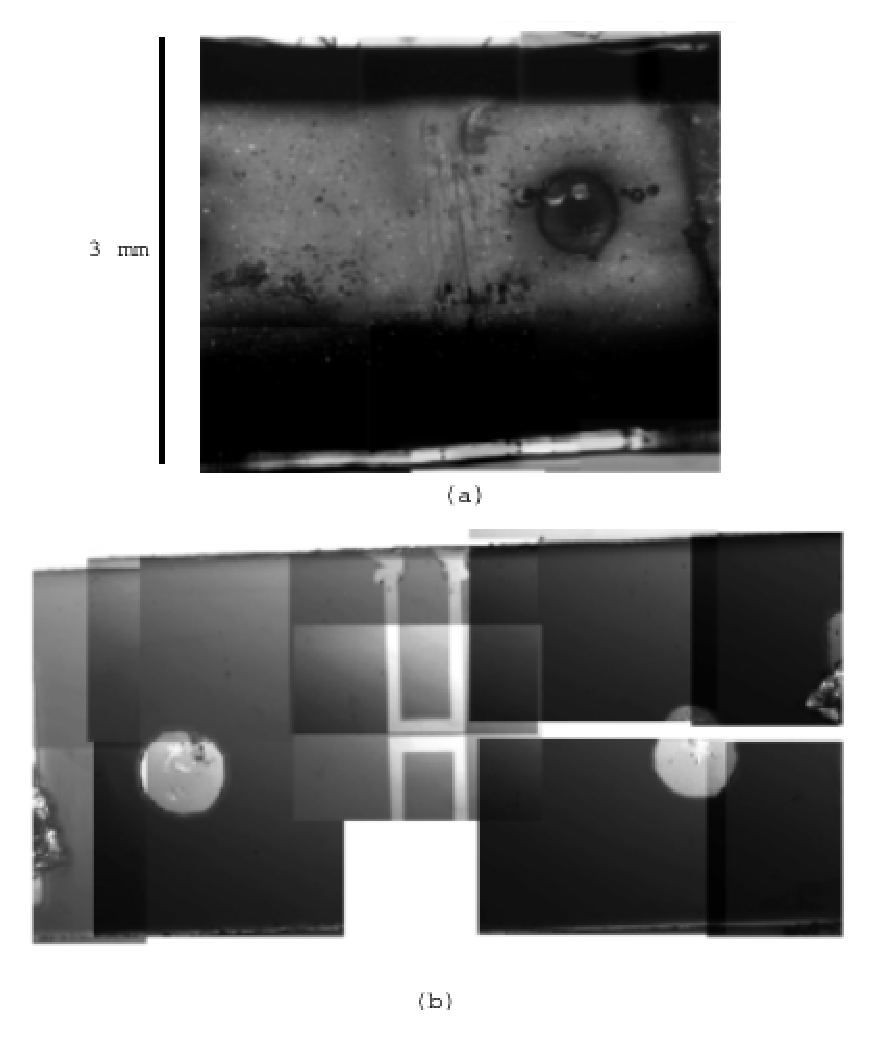
\includegraphics[height=6.0in]{figs/magpen/fig1.ps}
\caption[Optical micrographs of YBCO deposited on RABiTS and STO.]
{(a)Optical micrograph of YBCO deposited on RABiTS. The grains
are observable and are about $50\,\micron$ across. Additionally,
there are small holes evident in the film. These small holes
are approximately $100\,\micron$ apart.
(b) Optical micrograph of YBCO deposited on STO. There are none 
of the pin holes evident in the RABiTS image. This sample has a
microbridge for transport measurements, patterned into the center
via chemical etching. These are montage images, formed from several
different pictures: straight horizontal and vertical lines are
artifacts and not real features of the samples. }
\label{fig:optical_rabits}
\end{figure}

\subsection{Magnetic penetration into YBCO films}

Because RABiTS samples are deposited on nickel, they are 
ferromagnetic from room temperature down to $4.2\,\kelvin$. 
In order to distinguish properties of the YBCO films
from properties of the RABiTS we also looked at magnetic penetration into 
YBCO films 
deposited on STO.
%\footnote{The results of this study of magnetic
%penetration into YBCO films have lead to one publication, 
%Ref.~\cite{nielsen_magpen}.}
An optical image of this sample is shown in \MultFigRef{fig:optical_rabits}{b}.
This particular sample%
\footnote{ORNL sample designation \texttt{la100899}.} 
is YBCO deposited on STO using the same
deposition parameters used in making the YBCO on RABiTS sample 
discussed previously. Additionally, the YBCO/STO sample has been
etched in the center to form a small microbridge in the center. 


%
% Geometry discussion
%
For our discussions, we use the sample geometry defined in 
Fig.~\ref{fig:geometry}, in which we apply the magnetic field
along the $z$ axis, parallel to the thickness $d$ of the film. 
The width of the sample extends from $-W < x < W$ and the length
of the sample extends in the $y$ direction.

%
% fig2 - sample geometry
%
% sample geometry
% this geometry figure was not in the original paper outline,
% but seems useful to describe what's going on. 
%
\begin{figure}[p]
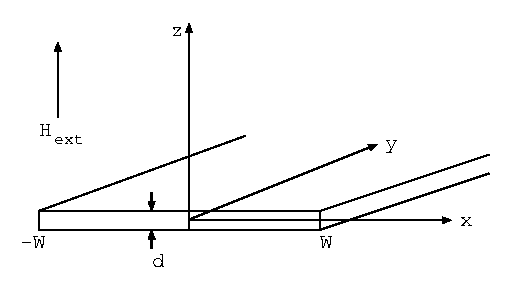
\includegraphics{figs/magpen/fig2.eps}
\caption[Sample geometry used magnetic penetration experiment analysis.]
{Sample geometry used in the experiment and discussion.
The external field is applied along the $z$-axis, through the 
thickness of the film $d$. The sample width extends from $-W < x < W$,
$W=1.5\,\mathrm{mm}$
and we treat the sample as infinitely long in the $y$ direction. 
}
\label{fig:geometry}
\end{figure}


\afterpage{\clearpage}

There has been significant theoretical 
discussion of this problem, in several different limits related
to the film thickness and width. 
In the extreme thin film limit (film 
thickness much less than the penetration depth) Larkin and Ovchinikov
\cite{larkin_jetp_34_651_1972} made the first calculations 
and derived the integral equations necessary to be solved for 
the current distribution in the Meissner state. 
The geometry is as described above, with the sample infinitely
long in the $y$ direction, and a current distribution 
dependent only upon $x$. 
Dorsey \cite{dorsey_prb_51_15329_1995}  took the
integral equations and derived analytic results valid over the 
entire width of the 
superconductor. For thicker films (film thickness comparable
to or larger than the penetration depth) Brandt
\cite{brandt_prl_71_2821_1993,brandt_prb_49_9024_1994,brandt_prb_54_4246_1996}
and Brandt and Mikitik \cite{brandt_prl_85_4164_2000} have made 
considerable numerical progress in describing the current distributions
over the cross-section of a superconducting slab and finally
Vodolazov and Maksimov \cite{vodolazov_physc_349_125_2001} have computed
analytic expressions for the current distributions. Up to now,
there have been no reported measurements of the current distribution
nor magnetic field distribution
in superconducting films
in the Meissner state.

The onset of flux penetration into a superconducting slab has also
been of considerable interest. There exists a large body
of theoretical work, from the geometrical barrier ideas of 
Zeldov \etal\,\cite{zeldov_prl_73_1428_1994} to the edge 
pinning ideas of Kuznetsov \etal\,\cite{kuznetsov_prb_59_1507_1999}
which discuss remanence in a superconducting slab. 
Furthermore, there have been experimental studies of the Bean
critical state in a superconducting slab by Johansen \etal\,
\cite{johansen_prb_54_16264_1996} using magneto optical indicator
\index{magneto optical indicator films}
films (MOIF) and by Ferdeghini \etal\,\cite{ferdeghini_physc_294_233_1998} 
\index{Hall probe}
using a scanning Hall probe. (Because of the large demagnetizing 
factor, initial flux penetration occurs for very low applied fields
and neither of
these techniques are sensitive to fields in this range.)

%
% RABITS
%

\section{YBCO on RABiTS}
\index{RABiTS|(emph}

RABiTS tapes are primarily nickel
\cite{feldman_apl_77_2000,feldman_2000,rabits_web} and it has been
previously reported that they contain a Landau type domain 
structure \cite{landau_physzs_8_153_1935,kercher_prb_60_6878_2000} 
in their 
cross-section. It is now known that this domain structure
cannot exist \cite{arrott_physb_233_259_1997,hertel_prb_60_7366_1999}, 
so we do not expect to find
this type of domain structure. In fact, we do not find any sort of 
simple magnetic domain structure. We imaged a RABiTS substrate%
\footnote{ORNL sample designation \texttt{n020898}.}
without any
superconducting layer deposited, shown in \FigRef{fig:naked_rabits},
and we estimate the height of the SQUID to be between fifty and 
one hundred micrometers for this scan.  
It is clear from the image that the sample is tilted with respect
to the plane of the SQUID.
In the image, the signals
are much clearer and stronger near the right side of the image, but 
fade out near the left edge of the sample. (We know 
the sample is tilted by making contact with the SQUID at 
different points and noting the difference in contact height.)
The magnetic image clearly demonstrates that the spontaneous
magnetization of the RABiTS film is very complicated. 
We did not attempt to demagnetize or magnetize the substrate in any
particular fashion because we wanted to image
the sample as it would (presumably) be if it were used commercially,
as there is no discussion of special magnetic preparation in the 
literature. 

%
% fig3 - naked rabits magnetic picture
%
\begin{figure}[p]
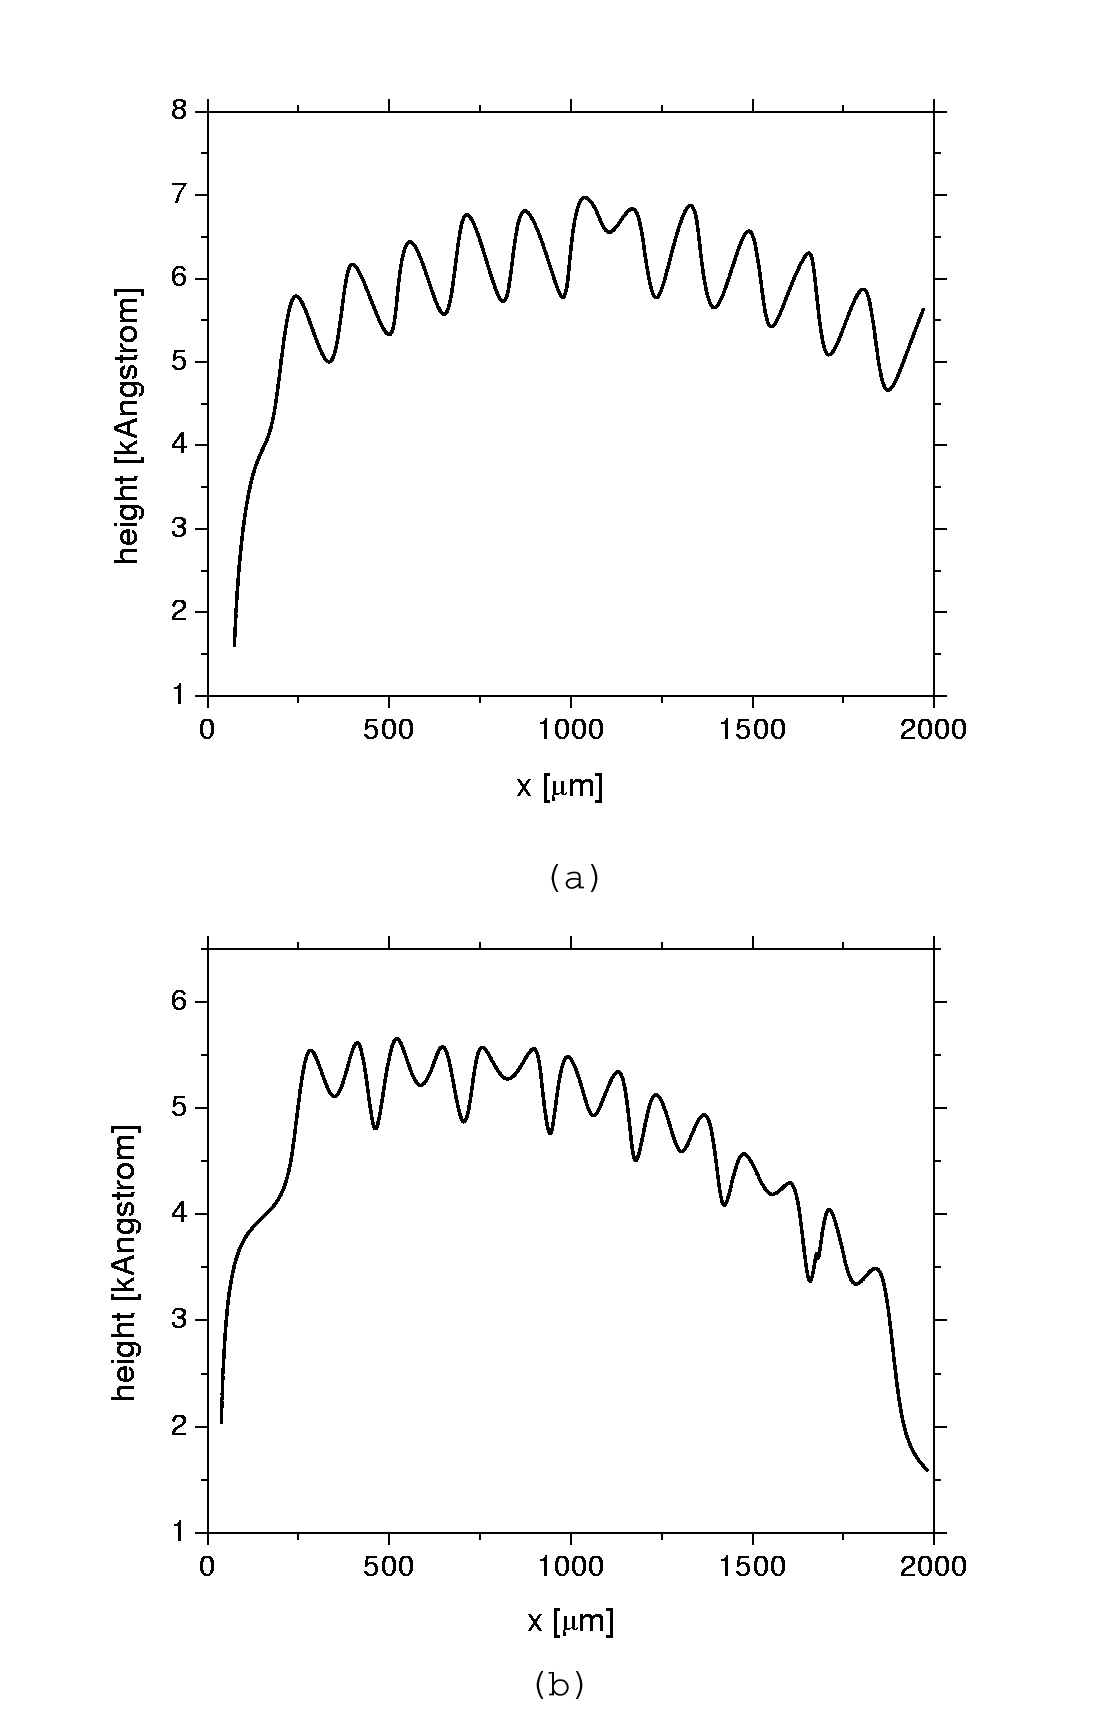
\includegraphics{figs/magpen/fig3.ps}
\caption[Magnetic image of bare RABiTS substrate.]
{Magnetic image of bare RABiTS substrate with spatial units along the
axes shown in millimeters.  The grey scale ranges from
black (low) to white (high) with a difference of  $6.75\,\Gauss$.
The image was taken at $4.2\,\kelvin$. The SQUID height is not 
constant over the surface of the sample; it is closer on the right,
and farther away on the left.}
\label{fig:naked_rabits} 
\end{figure}

Because of these measurements we realized that, using this type of 
substrate, we would be able to cool the sample in zero
\emph{external} field, but that the superconductor would always
see an extremely strong field due to the magnetization of the substrate. 
Hence, the superconductor deposited on RABiTS cannot be cooled in 
zero field.
We demonstrate this by showing, in \FigRef{fig:rabits_zfc},
a nominally zero-field cooled image of YBCO deposited onto RABiTS. 
There have been reports claiming to observe a geometrical barrier
\cite{zeldov_prl_73_1428_1994} in YBCO/RABiTS
\cite{kercher_prb_60_6878_2000}. However, it is not clear that this
should be the case since the YBCO film on RABiTS never sees 
a uniform external field, and further because of the holes in the 
sample we expect flux pinning to be quite strong; the geometrical
barrier requires extremely weak pinning (it was first observed in
single crystals). 

Because of the impossibility of zero field cooling, we
decided to look at YBCO deposited onto STO instead of the 
RABiTS tapes,\footnote{See section~\ref{sec:magpen_ybco},
p.~\pageref{sec:magpen_ybco}.} and investigate the existence of the
geometrical barrier.

\index{RABiTS|)}

%
% fig4 - ZFC YBCO on RABiTS
%
\begin{figure}[p]
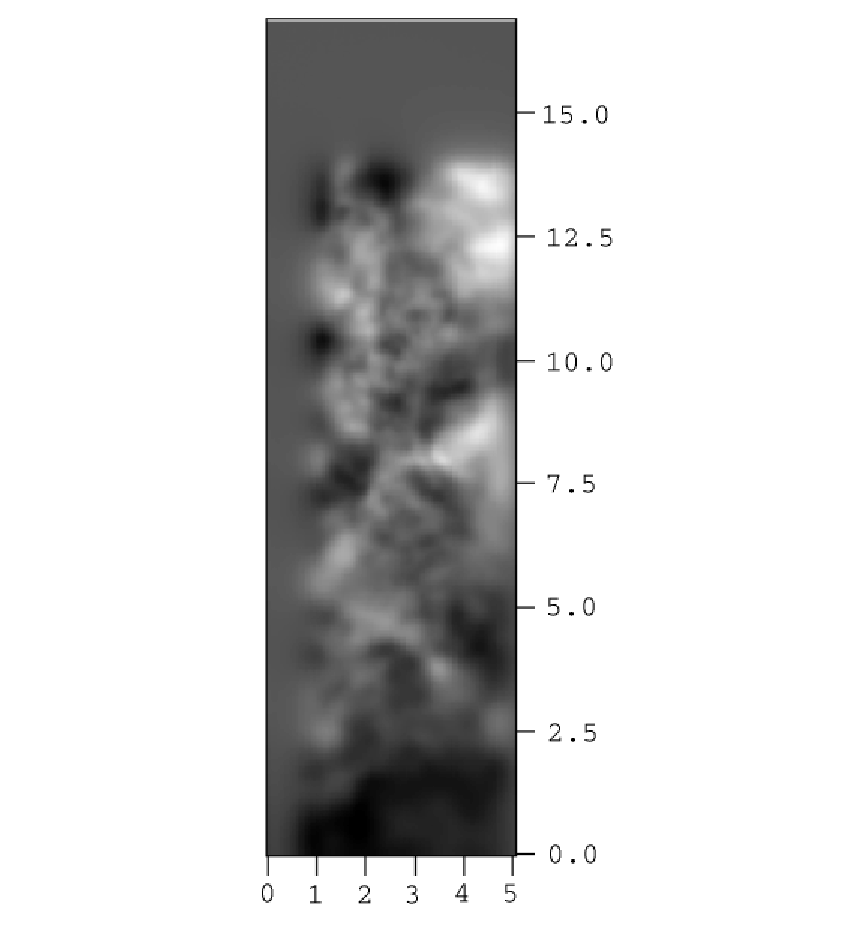
\includegraphics{figs/magpen/fig4.ps}
\caption[Magnetic image of zero field cooled YBCO on RABiTS.]
{Magnetic image of YBCO on RABiTS, cooled in zero external field
to $4.2\,\kelvin$, with the spatial units along the axes shown
in millimeters. 
The grey scale runs from black (low) to white (high) with a 
range of $4.75\,\Gauss$. The plane of the sample is tilted
with respect to the plane of the SQUID, causing the SQUID to 
be closer to the sample in the right of the image. This causes
the image to appear washed out at the left hand side of the image.}
\label{fig:rabits_zfc}
\end{figure}

%
% AC susceptibility measurements. 
%
\subsection{RABiTS AC susceptibility}
\index{AC susceptibility|(emph}
\index{RABiTS!AC susceptibility}
\label{sec:rabits_ac_sus}

In order to understand the basic mechanism involved with loss in
YBCO on RABiTS when carrying current, we used the SQUID to perform a local
measurement of the AC susceptibility at $500\,\Hz$ and 
$1\,\kHz$. 
We use the same experimental arrangement shown in 
\FigRef{fig:pme_experimental_setup}, except that instead of 
applying a DC field with the solenoid, we apply an AC field. 
We use an EG\&G model 5210
lock-in amplifier\cite{EGG} to measure the applied frequency
component in the output from the SQUID electronics. 
From the 
lock-in amplifier we acquire two spatially resolved signals, 
the in phase component and the out of phase component

We can relate these two components to the real and imaginary parts
of the AC susceptibility for the sample. In general the susceptibility is
defined from 
$\vec H = \vec {\vec \chi} \vec M$, in which $\vec{ \vec \chi}$ is the 
susceptibility, a tensor quantity,
$\vec H$ is the magnetic field, $\vec M$ is the magnetization
of the sample. If we assume that material is linear and isotropic, then 
$\chi = H/M$ and for a superconductor in the Meissner state
$\chi=-1$.\footnote{We strive to use MKS units, in which the proper
field relationship for various magnetic quantities is 
$\vec B=\mu_0(\vec H+\vec M)$,
throughout this 
discussion. A very useful chart for conversion between different
electromagnetic unit systems is in Jackson \cite{jackson}, p.~819.}

The sample sees an external driving field of
%
\begin{equation}
H_{\mathrm{ext}}(t) \, \hat z = H_{\mathrm{ac}}\cos(\omega t)\, \hat z
\end{equation}
%
The $\hat z$ component of the sample magnetization 
may be expressed as a series of
Fourier components related to the drive frequency, $\omega/2\pi$,
%
\begin{equation}
M(t) = H_{\mathrm{ac}} \sum_{n=1}^{\infty} 
\left[ \chi_n' \cos (n \omega t) - \chi_n'' \sin (n \omega t) \right]
\end{equation}
in which $\chi_n=\chi_n' + \mi \chi_n''$ is the complex susceptibility
at each frequency component, $n\omega/2\pi$. 
We discuss only the first component, $n=1$,
(hereafter referred to as $\chi$) though 
harmonic generation has been studied in some detail by others 
in bulk measurements
\cite{ishida_prb_41_8937_1990,yamamoto_prb_46_1122_1992}. 

We measure with the lock-in amplifier two components at the driving
frequency, $\omega/2 \pi$, one which is in phase with the driving 
field and one which is $\pi/2$ out of phase with the driving field.
These two components correspond to the real and imaginary 
components of $\chi$. 
The real part, $\chi'$,  corresponds to 
Meissner screening currents within the sample, which are not lossy and 
the imaginary part, $\chi''$, corresponds to processes which cause loss, 
eddy currents in the substrate and hysteretic process in the superconductor
or substrate. 
\index{AC susceptibility|)}

We used a driving amplitude of $223\,\mOe$ for these
measurements. A comparison of the sample response
is shown in \FigRef{fig:rabits_ac_images_a} and 
\FigRef{fig:rabits_ac_images_b} for two excitation
frequencies. 
The signals in these images consist of the YBCO
response and the nickel response. In general the response of both
the media must be considered together in a self-consistent manner, 
but we will discuss the effects separately first and some simplifications
to the self-consistent problem second. 


%
% fig5 part 1 - AC susceptibility images
%
\begin{figure}[p]
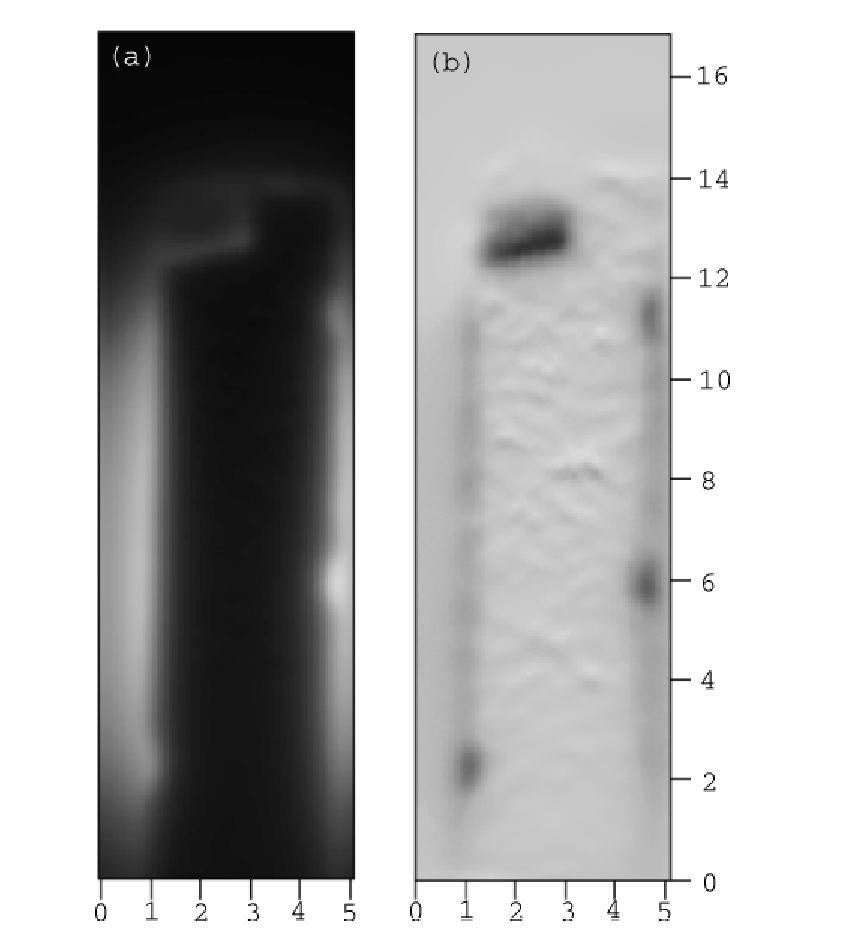
\includegraphics{figs/magpen/fig5r3a.ps}
\caption[YBCO on RABiTS AC susceptibility images at $1\,\kHz$.]
{AC susceptibility images for the YBCO on RABiTS sample, 
zero-field cooled to $4.2\,\kelvin$, 
for an external excitation frequency  
$1\,\kHz$ and
an amplitude of $223\,\mOe$
The spatial dimensions along both 
axes are in millimeters. 
(a) The $\chi'$ image whose grey scale ranges from
$-0.015\,\Gauss$ (black) to $0.25\,\Gauss$ (white).
(b) The $\chi''$ image whose grey scale ranges from  
$-0.045\,\Gauss$ (black) to $0.01\,\Gauss$ (white). 
}
\label{fig:rabits_ac_images_a}
\end{figure}

%
% fig5 part 2 - AC susceptibility images
% 	part 1 and 2 were split into two images to make the images 
%	end up larger when displayed. 
%
\begin{figure}[p]
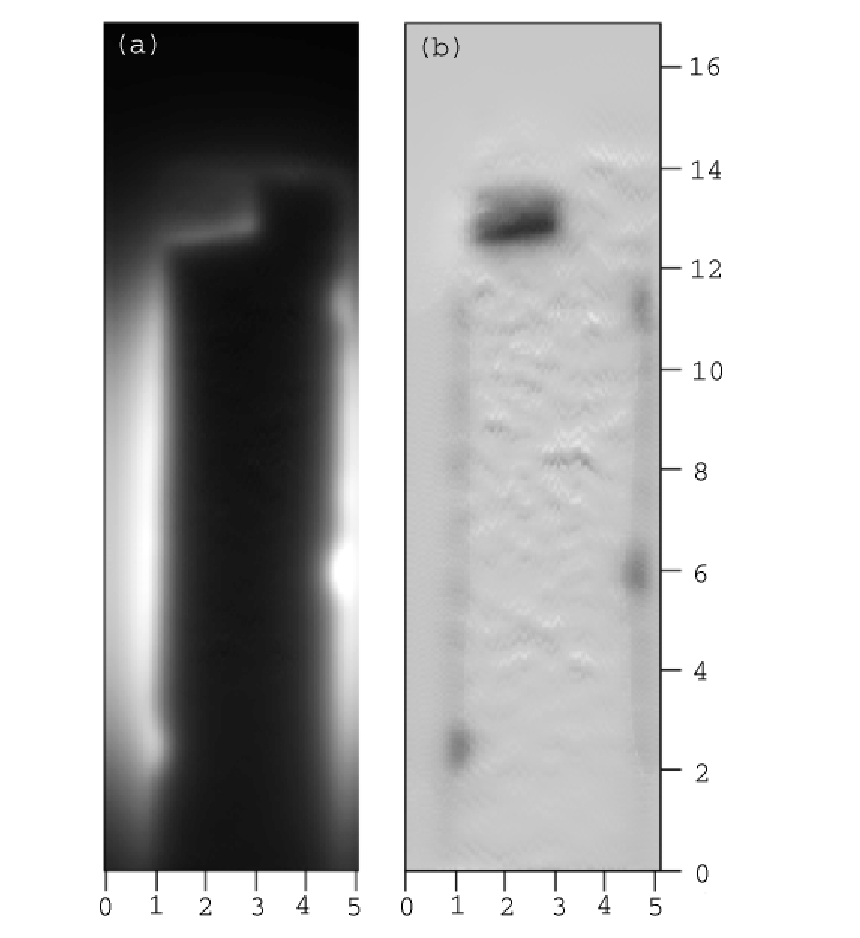
\includegraphics{figs/magpen/fig5r3b.ps}
\caption[YBCO on RABiTS AC susceptibility images at $500\,\kHz$.]
{AC susceptibility images for the YBCO on RABiTS sample, 
zero-field cooled to $4.2\,\kelvin$ for an external excitation frequency  
$500\,\Hz$ and
an amplitude of $223\,\mOe$. The spatial dimensions along both 
axes are in millimeters. 
(a) The $\chi'$ image whose grey scale ranges from
$-0.015\,\Gauss$ (black) to $0.25\,\Gauss$ (white).
(b)  The $\chi''$ image, whose grey scale ranges from
$-0.045\,\Gauss$ (black) to $0.01\,\Gauss$ (white). 
}
\label{fig:rabits_ac_images_b}
\end{figure}

We can understand the eddy current generation in the substrate by 
considering Maxwell's equations and Ohm's Law. 
We start by taking the curl of
Ohm's Law which gives
%
\begin{equation}
\nabla \times \vec{J}(\vec{x},t) = \sigma \nabla \times \vec{E}(\vec{x},t) 
= -\sigma 
{\dif  \over \dif t} \vec{B}(\vec{x},t) \mbox{.}
\label{eqn:eddy_curr_deriv}
\end{equation}
%
Additionally, we assume that the material response is linear 
so that
$\vec{B}(\vec{x},t) = \vec{B}(\vec{x})\me^{\mi \omega t}$
and $\vec{J}(\vec{x},t) = \vec{J}(\vec{x})\me^{\mi \omega t}$
which we substitute into \EqnRef{eqn:eddy_curr_deriv} to get
%
\index{eddy currents}
\begin{equation}
- \nabla \times \delta^2 \vec{J}(\vec{x}) = {\mi \over \mu_0} \vec{B}(\vec{x})
\label{eqn:eddy_current_screening}
\end{equation}
%
in which $\delta=\sqrt{1/\mu_0\sigma \omega}$ is the skin depth,%
\footnote{This skin depth differs from the skin depth as conventionally
defined by a factor of $\sqrt{2}$, see Jackson\cite{jackson}, p.~298 or 
Panofsky and Phillips\cite{panofsky_phillips}.}
$\mu_0$ is the permeability of free space, 
$\sigma$ is the 
conductivity of the material, $\omega/2\pi$ is the driving 
frequency, $\vec{J}(\vec{x})$ is the
induced eddy current and $\vec{B}(\vec{x})$ is the total magnetic induction. 
It's clear that the eddy current is out of phase with the 
drive field by a phase of $\pi/2$, which is why we expect the
field generated by the eddy currents to affect the $\chi''$ signal. 

It's interesting to note the similarity between 
\EqnRef{eqn:eddy_current_screening}\ and the London equation
(in MKS units)%
\footnote{See Tinkham\cite{tinkham}, p.~4 for the London equations.
We have neglected the time dependence 
of $\vec{J}$ and $\vec{B}$. In general these are time dependent 
quantities, but here we consider the DC Meissner response.}
%
\index{London equation}
\begin{equation}
- \nabla \times \lambda^2 \vec{J}(\vec{x}) = \vec{B}(\vec{x})
\label{eqn:London_equation}
\end{equation}
%
\index{London penetration depth}%
\index{$\lambda$|see{London penetration depth}}%
in which $\lambda$ is the London penetration depth, $\vec{J}(\vec{x})$ is the 
Meissner current and $\vec{B}(\vec{x})$ 
is the total magnetic induction. In our 
geometry, the shape of the current distribution $\vec{J}(\vec{x})$ will be 
the same for both \EqnRef{eqn:eddy_current_screening} and 
\EqnRef{eqn:London_equation}. The primary difference is that
the eddy current screening is out of phase with the drive field,
while Meissner current screening is in phase with the drive field
(and the Meissner current may flow at DC). 

As discussed above, we expect to see the eddy current response of the nickel
in the $\chi''$ image. However, the nickel is below (and hence
screened) by the YBCO, so we do not necessarily expect the 
nickel to actually see the driving field and respond,
except in regions where the YBCO fails to screen. 
In fact this is exactly what we see. 
In \MultFigRef{fig:rabits_ac_images_a}{a}, which shows
$\chi'$,
there is a light 
region in the upper right corner of the sample which does
not screen the external field. Darker colors are screening
regions in this case because they are closer to zero field.
This same region in 
\MultFigRef{fig:rabits_ac_images_a}{b}, $\chi''$, 
shows the strongest response 
indicating that the YBCO is not superconducting in 
this region and hence not screening the nickel tape underneath. 
In addition to this region, there are other regions which have the 
same correlation between the two images, particularly at the edges of 
the sample.

We can understand these measurements more quantitatively by 
considering separately the AC response of the YBCO and the nickel
substrate. At our low temperature ($4.2\,\kelvin$) and field amplitude
(below $H_{c1f}$),
we expect the sample to be in the Meissner state, and so we expect to
observe Meissner shielding in phase with the driving field. 
We could not cool the sample in zero field due to the presence of the 
substrate. The substrate provides a DC magnetic field, if the pinning
in the sample is strong enough, this DC field will be pinned and
when we measure AC excitations of the sample, we expect to find
a Meissner screening response at the same frequency as the driving 
field.
Line cuts through the $\chi'$ magnetic images in 
\FigRef{fig:rabits_ac_images_a} and 
\FigRef{fig:rabits_ac_images_b}\ at $x=9.1\,\mm$ are shown in 
\FigRef{fig:rabits_ac_line_cuts_a}, and qualitatively show the expected
Meissner screening form.\footnote{We discuss Meissner screening
in great detail in section \ref{sec:ybco_meissner_state}, 
p.~\pageref{sec:ybco_meissner_state}. We note here that these
AC susceptibility measurements agree with the Meissner state
discussion below.} 

%By considering the images, several features become immediately
%obvious. We can see that there appears to be some form of damage to 
%the sample, degrading the superconductivity in the sample when
%we compare \FigRef{fig:rabits_ac_images}. Consider the dark
%regions in \FigRef{fig:rabits_ac_images}(b) and (d) which indicate
%that the sample is lossy. These regions correspond to regions in 
%\FigRef{fig:rabits_ac_images}(a) and (c)  in which there 
%is no screening response. All of these regions occur near the 
%edge of the sample, indicating that there has been some 
%damage to the sample near the edges, causing the loss of 
%superconductivity in those regions. It is likely that these lossy 
%regions are actually the nickel eddy current response, as
%discussed above. 

%
% recombine these into one figure
%
\begin{figure}[p]
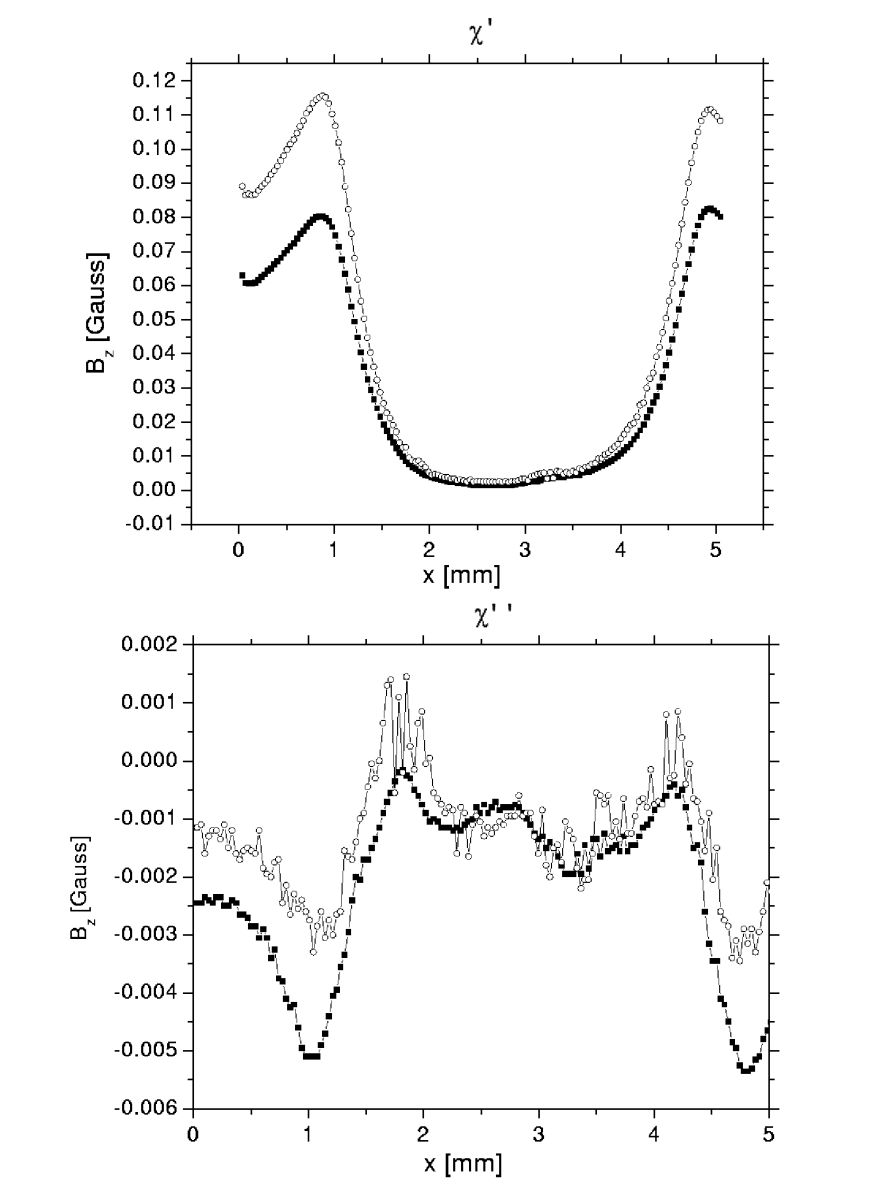
\includegraphics[width=5.7in]{figs/magpen/ac.ps}
\caption[$\chi'$ and $\chi''$ line cuts through AC 
susceptibility measurements.]
{$\chi'$  and $\chi''$ 
line cuts through AC susceptibility measurements taken at 
$x=9.1\,\mm$, for $1\,\kHz$ (black squares) and
$500\,\Hz$ (open circles).
}
\label{fig:rabits_ac_line_cuts_a}
\label{fig:rabits_ac_line_cuts_b}
\end{figure}

%  part 1
% line cuts through ac sus images
%
%\begin{figure}
%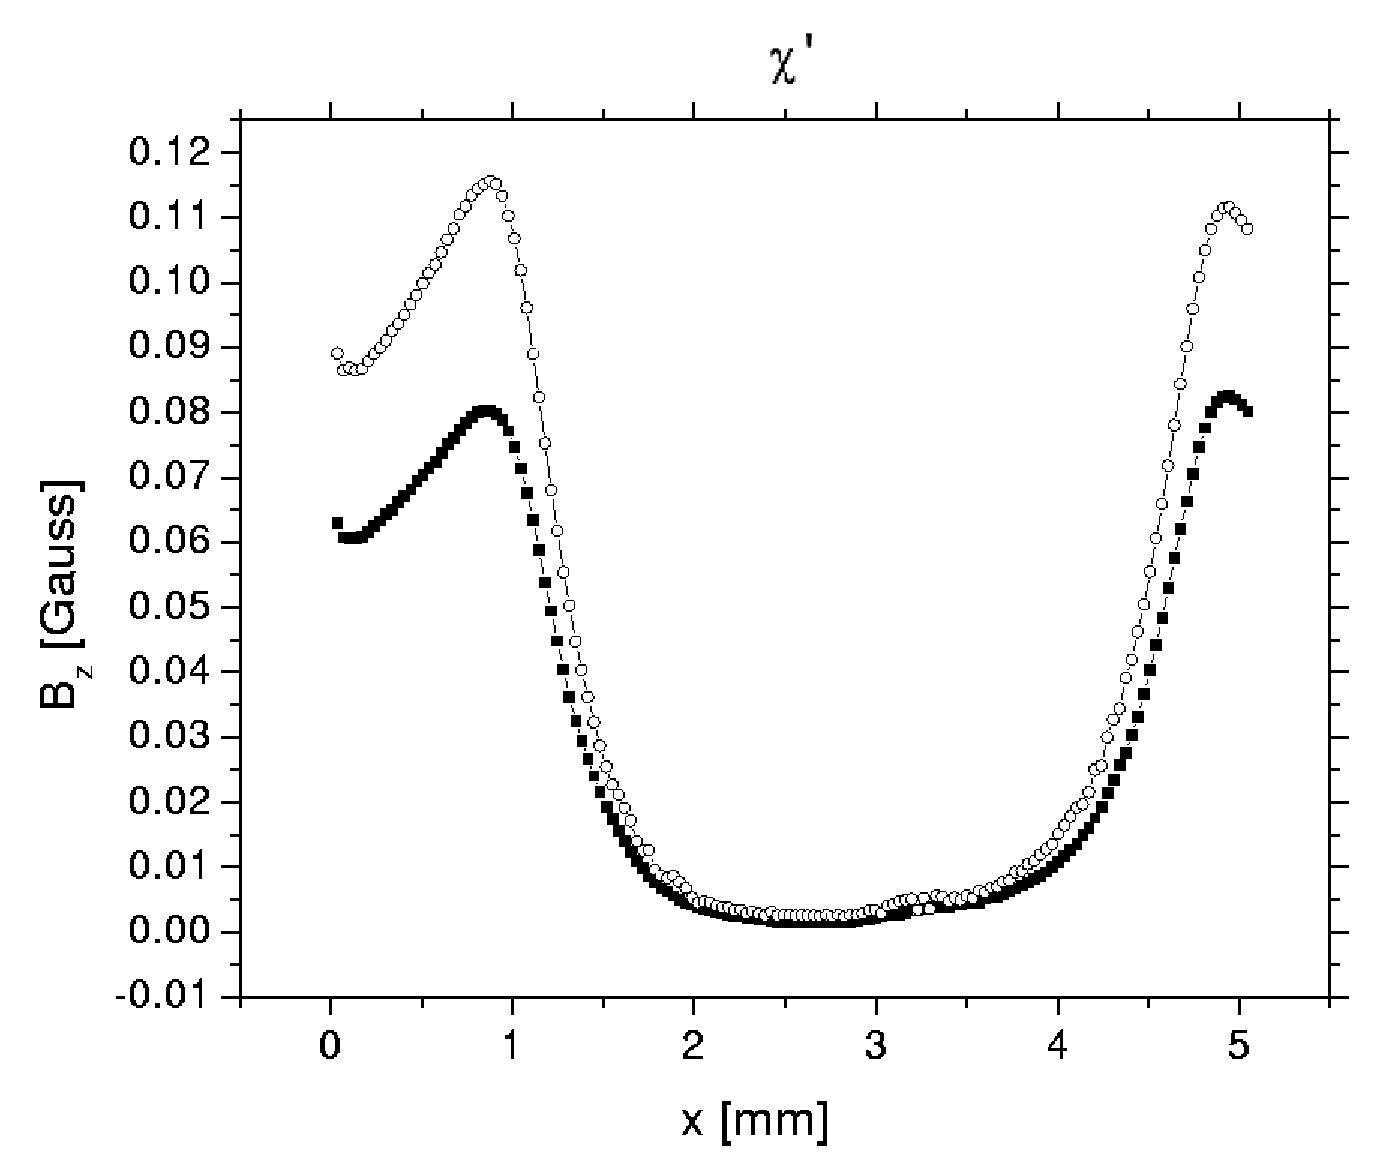
\includegraphics[width=5.7in]{figs/magpen/acinphase.ps}
%\caption[$\chi'$ line cuts through AC susceptibility measurements]
%{$\chi'$ line cuts through AC susceptibility measurements taken at 
%$x=9.1\,\mm$, for $1\,\kHz$ (black squares) and
%$500\,\Hz$ (open circles).
%}
%\label{fig:rabits_ac_line_cuts_a}
%\end{figure}

%  part 2
% line cuts through ac sus images
%
%\begin{figure}
%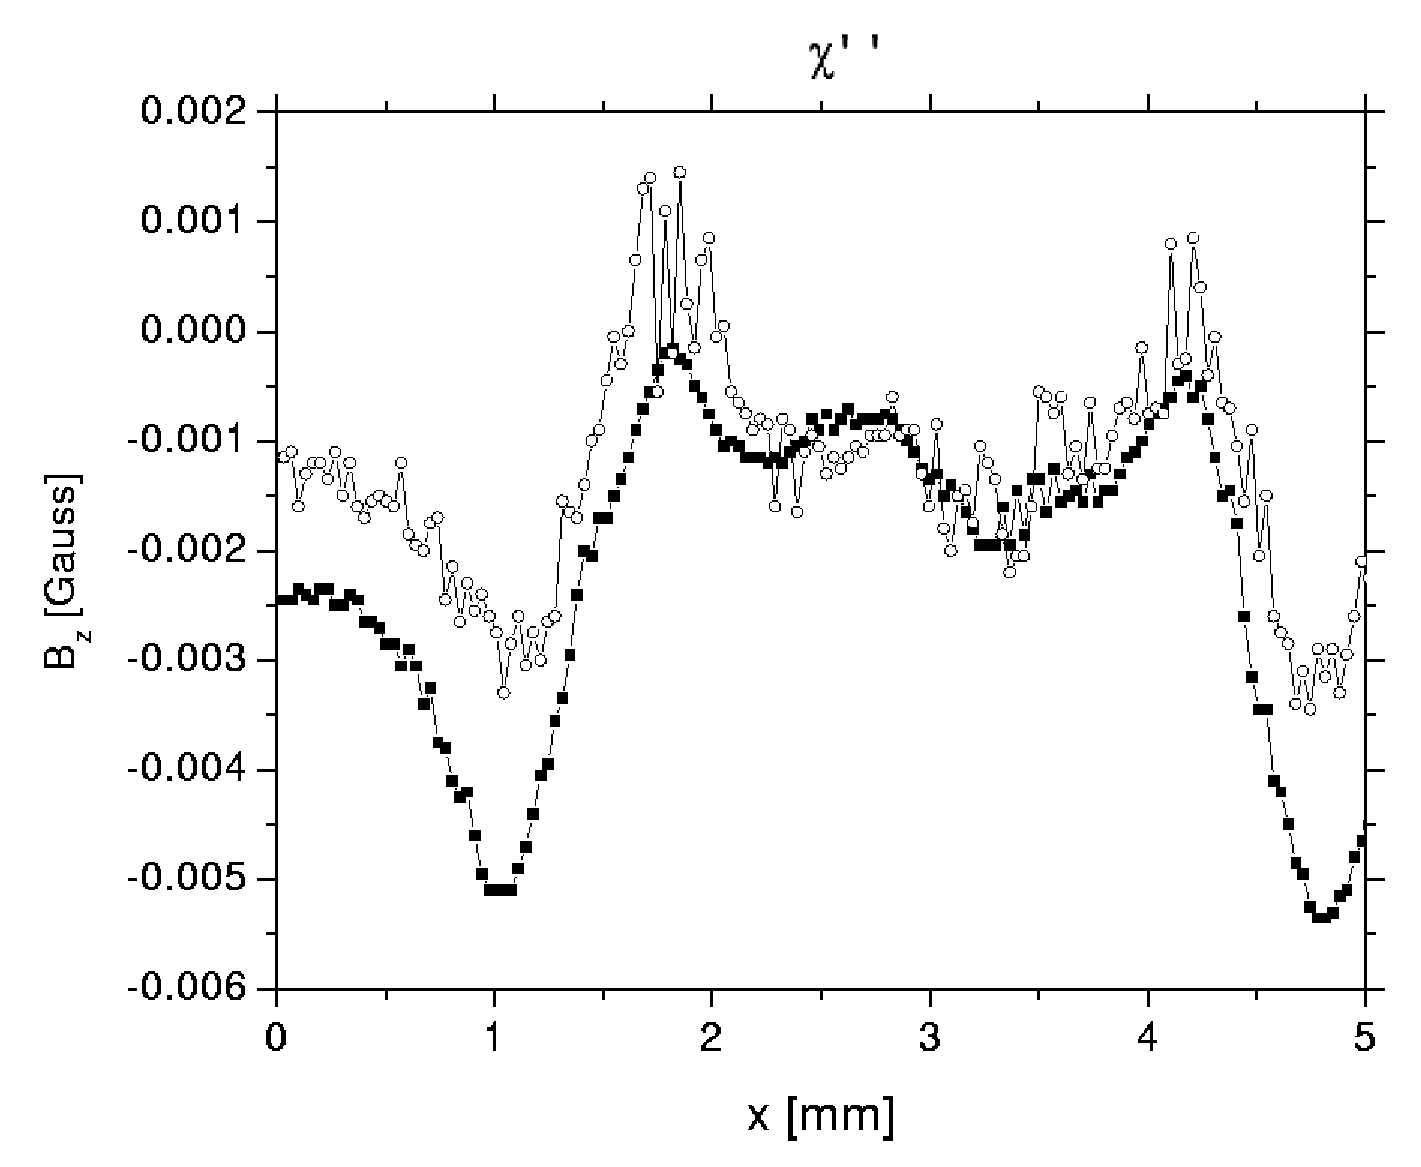
\includegraphics[width=5.7in]{figs/magpen/acoutofphase.ps}
%\caption[$\chi''$ line cuts through AC susceptibility measurements]
%{$\chi''$ line cuts through AC susceptibility measurements taken at 
%$x=9.1\,\mm$, for $1\,\kHz$ (black squares) and
%$500\,\Hz$ (open circles).}
%\label{fig:rabits_ac_line_cuts_b}
%\end{figure}

\label{sec:flux_motion_losses}
In the superconductor itself, we expect to observe losses associated
with motion of flux
for any, arbitrarily low, excitation
field because the spontaneous magnetization of the nickel assures
that flux will always be present in the superconductor. 
Losses due to vortex motion in a superconductor may result 
from different processes, flux-flow resistance
\cite{nikolo_prb_39_6615_1989,clem_mag_sus_1991} and
intergranular (or grain boundary) vortex motion
\cite{celebi_physc_309_131_1998,muller_prb_43_7976_1991}.
It is well known that flux-flow resistance is strongly dependent
upon driving frequency.\footnote{An analogy can be drawn between 
flux-flow resistance and eddy current generation in normal metals,
which as discussed previously, is proportional to the driving 
frequency. See Clem \cite{clem_mag_sus_1991} for an excellent 
description and derivation of the analogy.} 
Moreover, it has been reported that losses due to intergranular 
vortex motion are typically frequency 
independent \cite{celebi_physc_309_131_1998}.

We pointed out previously that because of the large spontaneous
magnetization of the nickel that we could not 
cool the sample in total zero field,
so
we do not expect the sample to be in the Meissner state.
Instead we expect the sample 
to have a complicated internal magnetic structure, which
will respond hysteretically to the excitation field. Hysteretic losses
appear in the out of phase image and provide a means to identify
lossy regions of the sample. Furthermore, by studying the amplitude
and frequency dependence we may determine the cause of the losses in
different regions. There are regions near
the edges of the sample which have strong loss signals, and no Meissner
screening signal. These regions are likely defective YBCO film
and the strong loss signal results from the eddy currents in the nickel. 

It is difficult to do a systematic study of the sample over a wide
frequency and amplitude range because of the time required to generate
the different images. None the less, we have made several images
at a fixed external amplitude, over a range of frequencies from
$500\,\Hz$ to $5\,\kHz$. A selection of these images is shown in 
\FigRef{fig:rabits_ac_images_a}\ and 
\FigRef{fig:rabits_ac_images_b}, with line cuts through these images at
$x=9.1\,\mm$ shown in \FigRef{fig:rabits_ac_line_cuts_a}
and \FigRef{fig:rabits_ac_line_cuts_b}. From the line
cuts in \FigRef{fig:rabits_ac_line_cuts_b} ($\chi''$ or loss images)
we notice that there is considerable internal structure and that 
both line cuts at $500\,\Hz$ and $1\,\kHz$ are remarkably similar. 
Furthermore, we notice that the line cuts do not go to zero outside of the
sample as they should. This indicates that the phase separation between
the in and out of phase signals was incomplete at the lock-in amplifier.
None the less, the loss signal is qualitatively 
frequency independent, indicating that
the losses are occurring at the grain boundaries, rather than in the grains. 

With losses occurring in the grain boundaries, rather than in the 
grains themselves (as flux-flow resistance) we expect that the current
carrying capacity of the YBCO on RABiTS films may be increased by increasing
the size of the grains in the sample. At some point however, the spontaneous
magnetization of the RABiTS substrate will become the limiting factor
for the losses, inducing flux in the YBCO causing flux-flow losses. 
These flux-flow losses would continue to occur even if one could 
engineer a way to deposit a single crystal on the RABiTS. 


%
% DC hysteresis measurements 
%
\subsection{RABiTS DC hysteresis measurements}
\label{sec:rabits_dc_hyst}
\index{DC susceptibility}
\index{RABiTS!DC susceptibility}

In addition to the AC susceptibility measurements we made DC 
hysteresis measurements on the sample in order to investigate
how flux became pinned in the sample. We did this measurement
at two different heights above the sample, approximately $50\,\micron$
and $20\,\micron$, but could only take single line scans at the
closer height because of a tilt in the mounted sample relative
to the scanning plane. 

To generate a hysteresis measurement we take one scan after
zero field cooling; ramp the external field up to a specific
value; ramp the field back to zero; and finally reimage the sample. 
We compare the two images by subtracting the first from the 
second. The resulting difference image should reveal where flux
trapping is hysteric for the particular field.

We show, in \FigRef{fig:dc_hyst_gen_a}(a)-(b) the images before
and after application of the external field and in 
\FigRef{fig:dc_hyst_gen_b}(a) the difference between 
\FigRef{fig:dc_hyst_gen_a}(a)-(b).
The SQUID at a height
between $100\,\micron$ (however, the sample is tilted, as discussed 
above for the bare RABiTS substrate) and  
$50\,\micron$ and a peak applied external field of $223\,\mOe$. 
In addition to the difference image, we compare the 
magnitude of the gradient of the field in 
\MultFigRef{fig:dc_hyst_gen_a}{a}\ $\left| \nabla_{x,y} B_z \right|$
(shown in \MultFigRef{fig:dc_hyst_gen_b}{b}) with the difference 
image in order to verify that the features observed in the 
difference image are not a result of mechanical misalignment
between the two images resulting in a false image.
We do this because two images, exactly the same, but offset slighly
will produce a difference image which contains the strongest
signal near where the gradient of the first two images is largest.
 It is clear 
from comparing \FigRef{fig:dc_hyst_gen_b} (a) and (b) that 
there is some correlation between the two images, indicating that some
of the structure is due to misalignment in the probe mechanics. 

%
% fig6 part 1 - DC hysteresis images
%	these figure numbers no longer refer to numbers in the 
%	text, but they do refer to figures as numbered in the
%	figure directory
%
\begin{figure}[p]
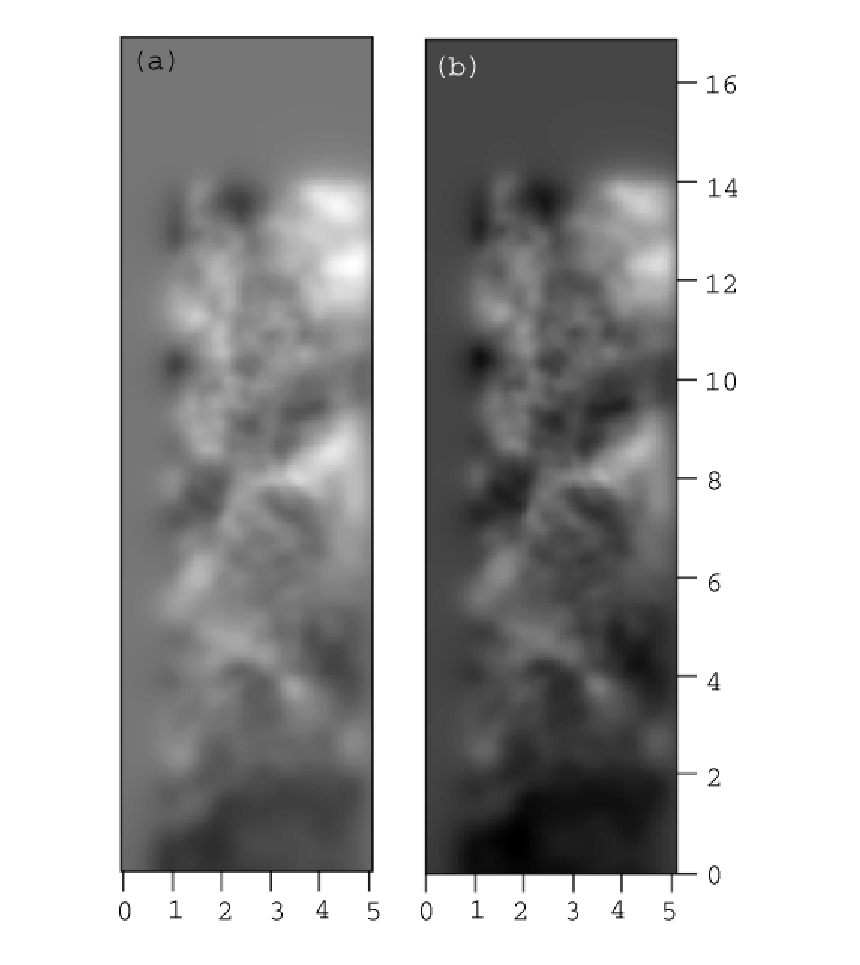
\includegraphics{figs/magpen/fig6a.ps}
\caption[DC hysteresis before and after images of YBCO/RABiTS.]
{Typical images used to study DC hysteresis in the YBCO/RABiTS data
at a height of $50\,\micron$.
(a) Image taken after zero field cooling the sample. The grey
scale ranges from low (black) to high (white) with a total
range of $5.6\,\Gauss$. 
(b) Image taken after ramping the external field to $1.16\,\Gauss$
and subsequently removing the external field before measuring. 
The grey scale is the same as (a). 
}
\label{fig:dc_hyst_gen_a}
\end{figure}

%
% fig6 part 2 - DC hysteresis images
% 	these were split into two parts to make them appear large
% 	in the text
\begin{figure}[p]
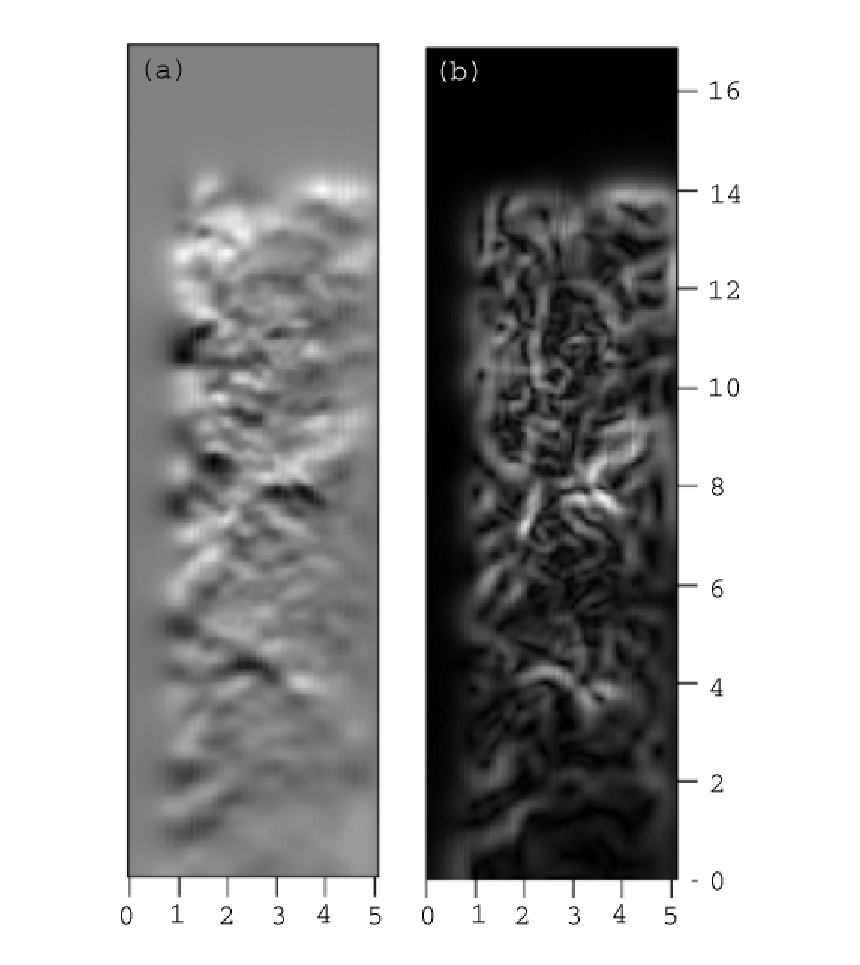
\includegraphics{figs/magpen/fig6b.ps}
\caption[DC hysteresis difference and gradient images of YBCO/RABiTS.]
{Typical images used to study DC hysteresis in the YBCO/RABiTS data
at a height of $50\,\micron$.
(a) Difference image taken by subtracting 
\FigRef{fig:dc_hyst_gen_a}(a) from (b), the grey
scale ranges from $-1.7\,\Gauss$ (black) to $-0.35\,\Gauss$ (white). 
(b) Magnitude of the gradient of the image in (a) for comparison 
with the difference image. The grey scale runs from zero (black) to
$7.3\,\Gauss/\mm$ (white).
}
\label{fig:dc_hyst_gen_b}
\end{figure}

A simple method to correct for this would be to shift one of the 
images in $x$ and $y$ before taking the difference, however
to simplify this comparison process, we took single vertical line scans over 
the sample at a horizontal point of $7.5\,\mm$ in \FigRef{fig:dc_hyst_gen_a}.
These single line scans were taken separately from the images discussed
above and were arranged so that the sample only moved along the single 
line during the data collection. In this way the line scans lie atop
each other and would only need to be shifted in one direction. 
These line scans, shifted to match the peaks 
are shown in \FigRef{fig:dc_hist_cuts_high_a}, 
for both the zero field cooled and hysteresis scans. 
It was not possible to match all of the peaks simultaneously. 
Vertical, numbered lines are drawn in \FigRef{fig:dc_hist_cuts_high_a}
at the location of several peaks. In order to correlate these two
line scans we shifted the curves such that peak 1 occurred at the same
$x$ value for each. After we did this, the location of peak 2 and 4
did not coincide, however the location of peak 3 did. The difference
in the peak coincidence,less than $10\,\micron$,  indicates that either 
the mechanical deviations are not linear across the scan or that
small flux has shifted within the sample on very small length scales. 
The difference 
between these two scan lines is shown in \FigRef{fig:dc_hist_cuts_high_b}
along with the gradient of the zero field cooled line scan for 
comparison. Both line scans are very similar, except for a 
small offset which may be due to a flux jump in the SQUID washer
between line scans.
Furthermore, the gradient of the line scans correlates quite
well with the difference between the two line scans, 
indicating that the difference we are 
measuring is a result of mechanical misalignment in the scanning 
mechanism, rather than real hysteresis. 

\begin{figure}[p]
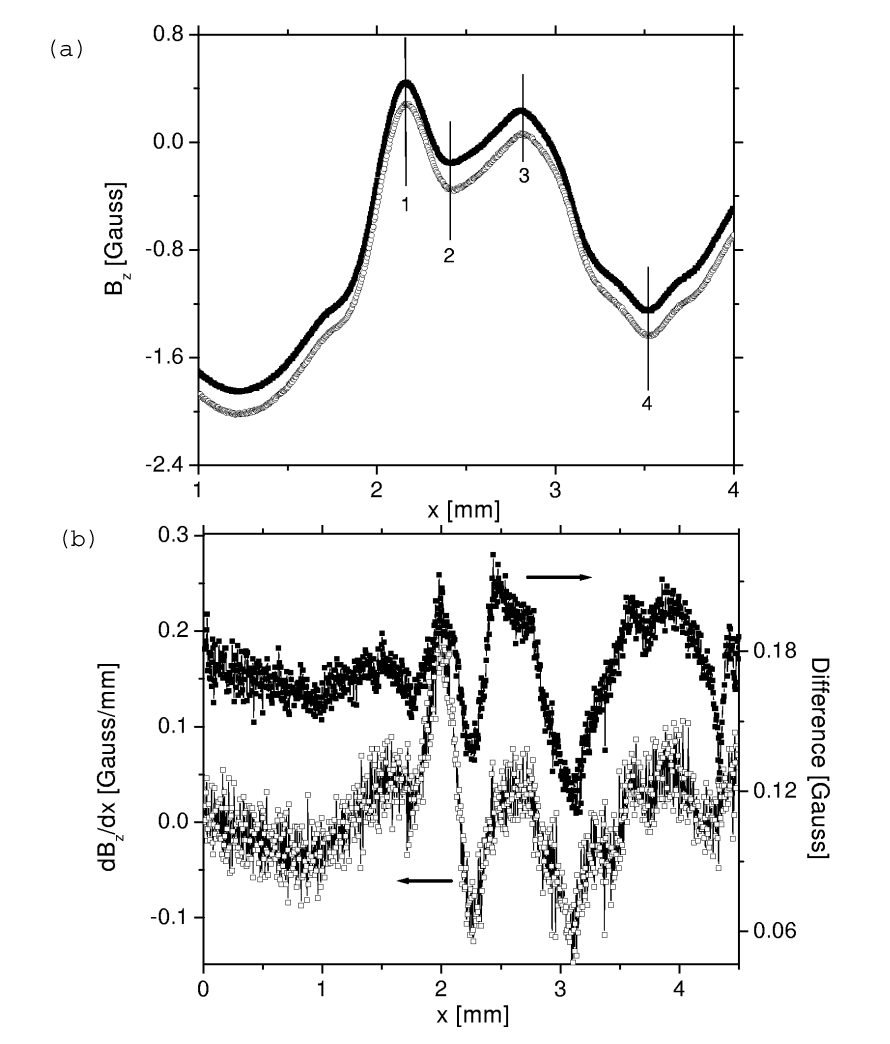
\includegraphics[width=5.7in]{figs/magpen/dcline.ps}
\caption[Before and after line cuts of DC hysteresis 
images at a height of $50\,\micron$.]
{(a) 
Vertical line cuts of DC hysteresis images, with the SQUID at a height of
$50\,\micron$, at $x=7.5\,\mm$. 
Zero field cooled line scan (open circles) and line scan after 
ramping the external field to $1.16\,\Oe$ and back to zero
(black squares). 
(b) Difference (black squares) and gradient (open squares) of the
vertical line cuts.
}
\label{fig:dc_hist_cuts_high_a}
\label{fig:dc_hist_cuts_high_b}
\end{figure}

%
% fig7 - line cuts of DC hysteresis images @ 50 microns
% part 1 - before and after line cuts
%
%\begin{figure}
%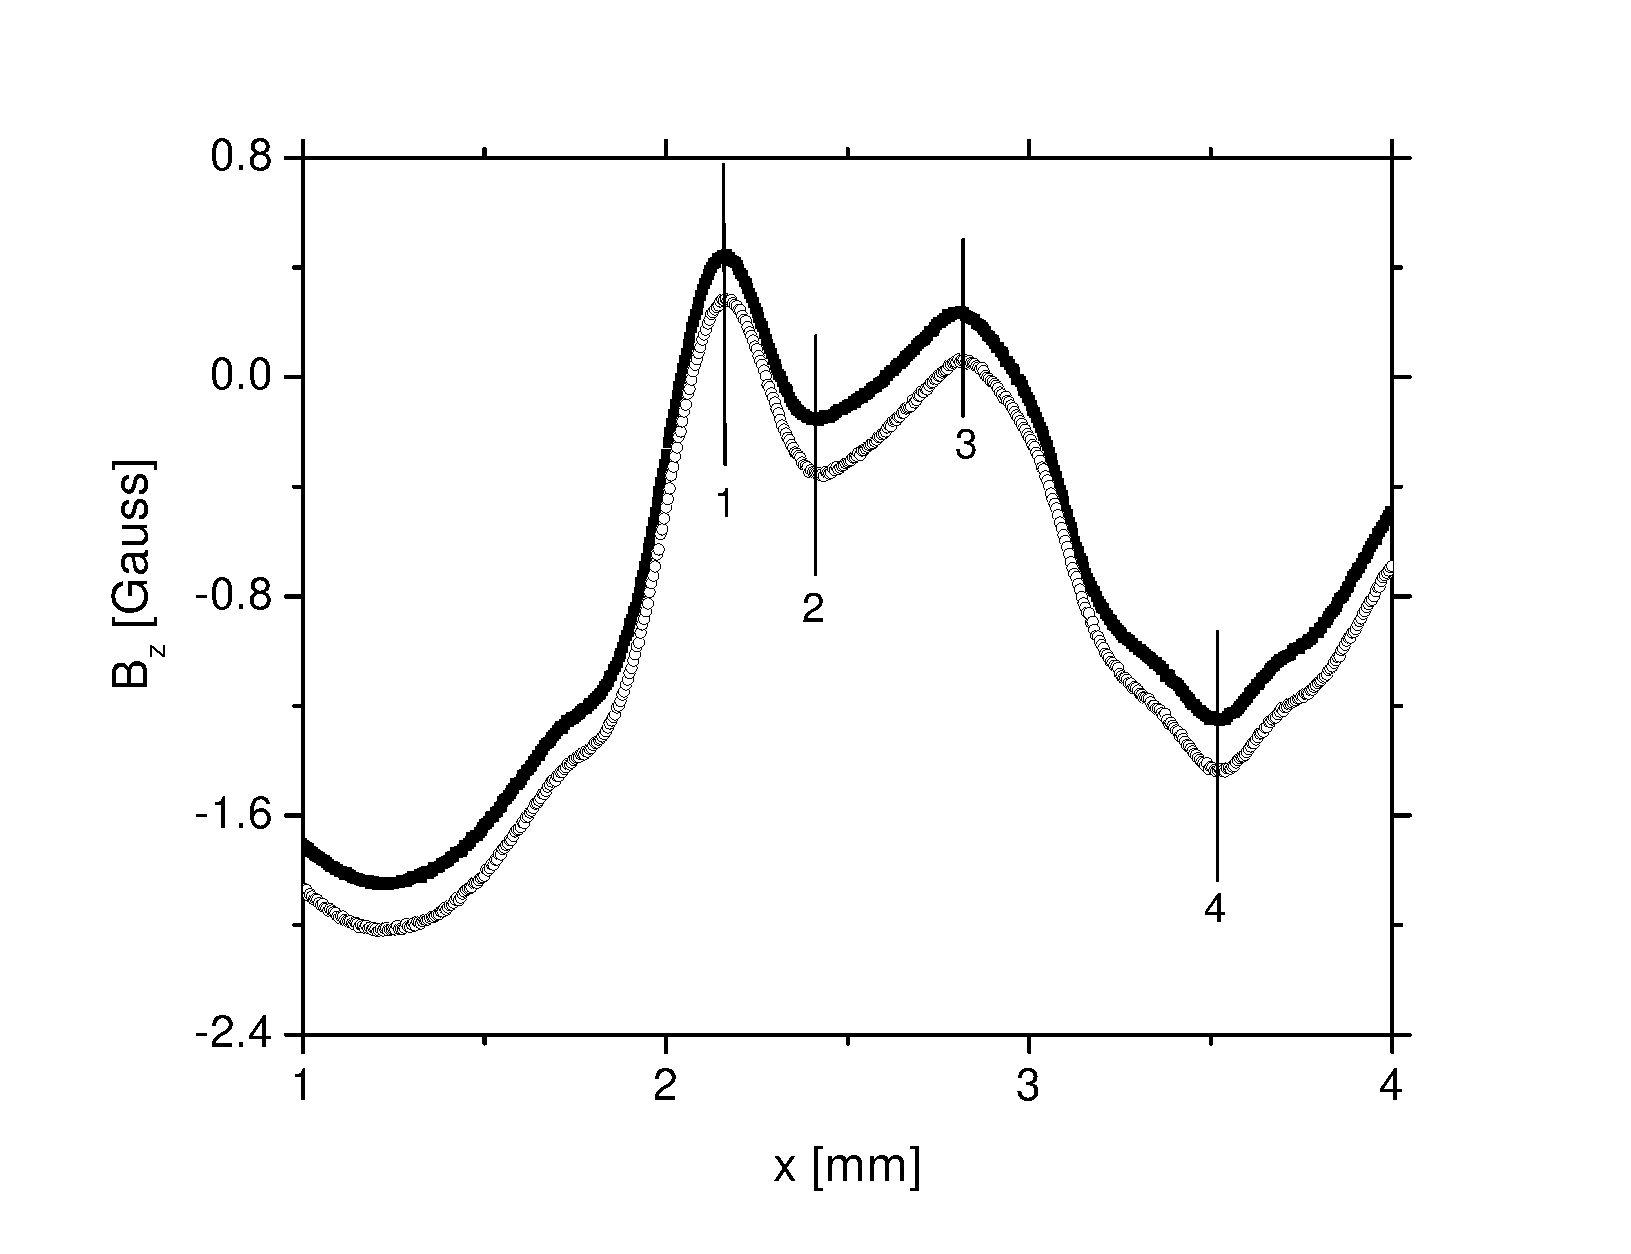
\includegraphics[width=5.7in]{figs/magpen/fig7a.eps}
%\caption[Before and after line cuts of DC hysteresis 
%images at a height of $50\,\micron$.]
%{Vertical line cuts of DC hysteresis images, with the SQUID at a height of
%$50\,\micron$, at $x=7.5\,\mm$. 
%Zero field cooled line scan (open circles) and line scan after 
%ramping the external field to $1.16\,\Oe$ and back to zero
%(black squares). 
%}
%\label{fig:dc_hist_cuts_high_a}
%\end{figure}

%
% fig7 - line cuts of DC hysteresis images @ 50 microns
% part 2  - difference and gradient line cuts
%
%\begin{figure}
%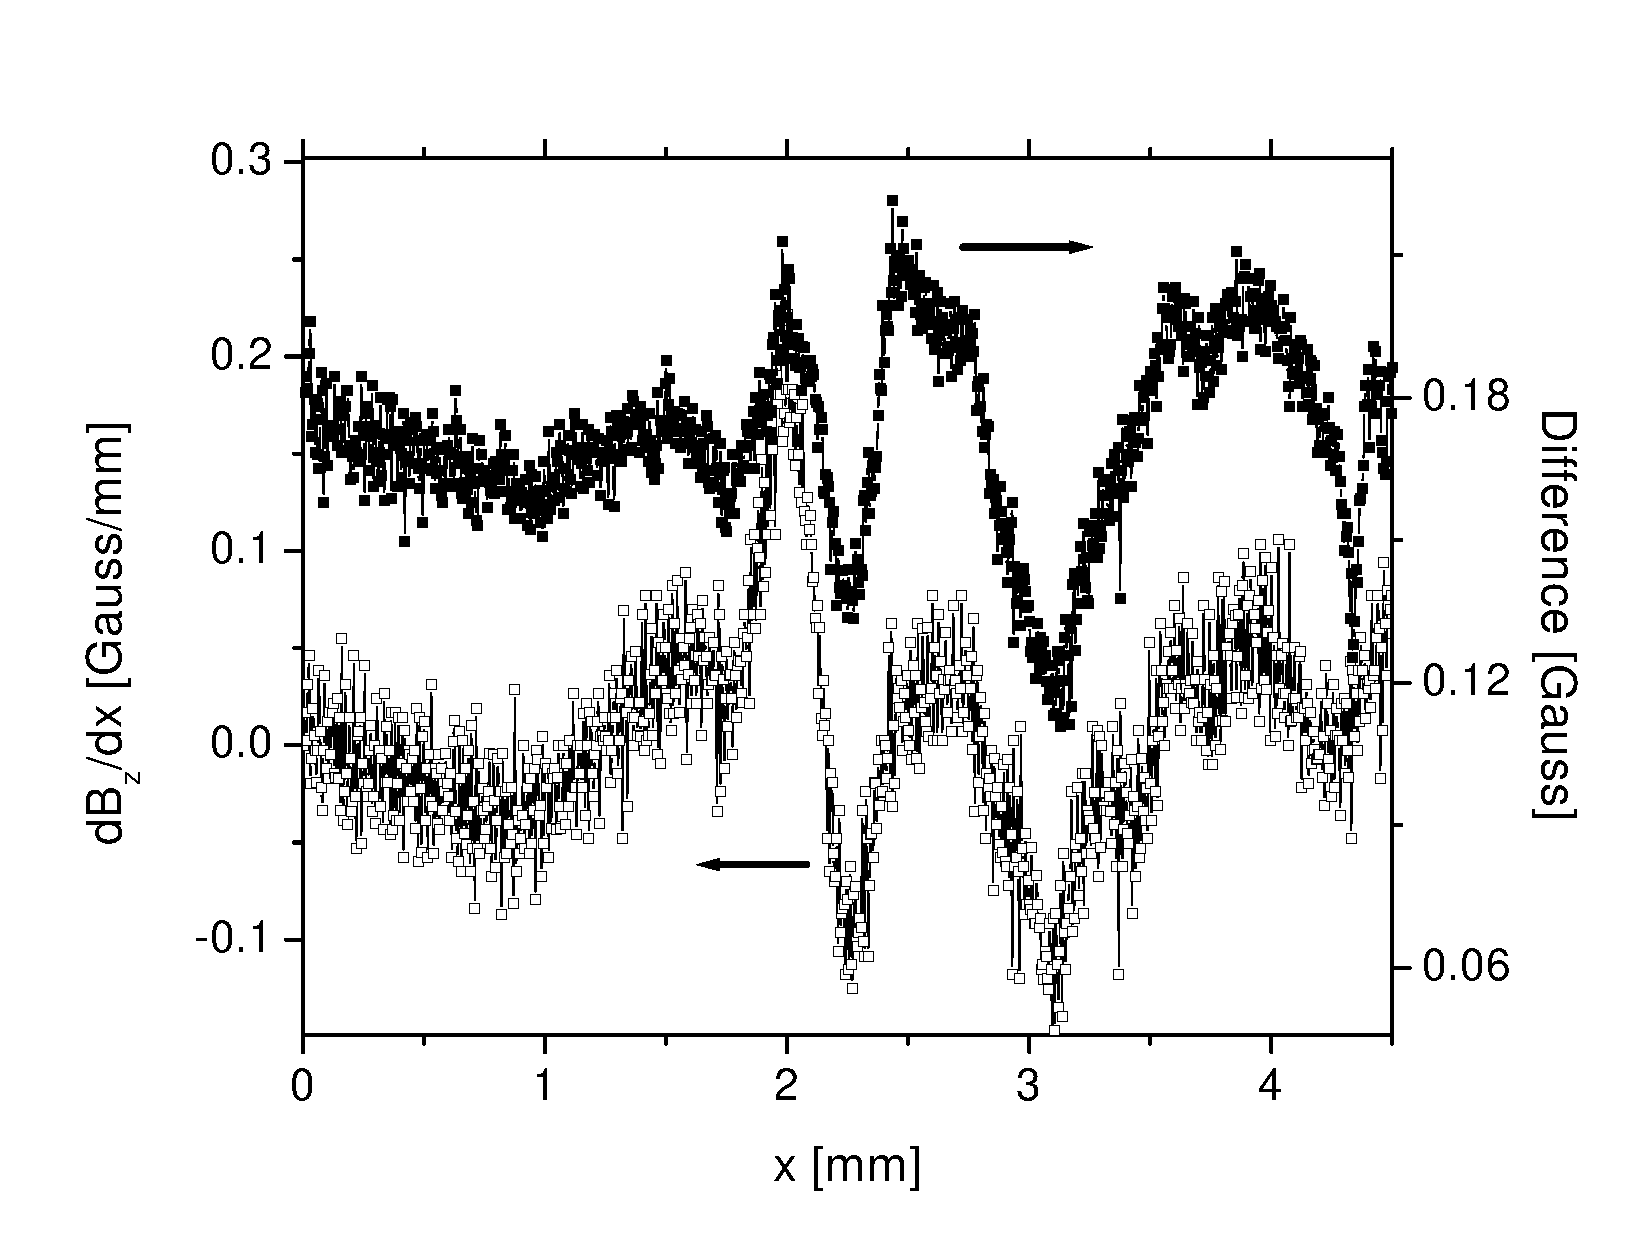
\includegraphics[width=5.7in]{figs/magpen/fig7b.eps}
%\caption[Difference and gradient line cuts of DC hysteresis 
%images at a height of $50\,\micron$.]
%{Vertical line cuts of DC hysteresis images, with the SQUID at a height of
%$50\,\micron$, at $x=7.5\,\mm$. 
%Difference of the two curves in \FigRef{fig:dc_hist_cuts_high_a} 
%(open squares) 
%and the derivative plot 
%of the zero field cooled line scan (black squares).  
%}
%\label{fig:dc_hist_cuts_high_b}
%\end{figure}

In order to improve upon the line scans taken above, we made 
line scans at 
a SQUID height of about $20\,\micron$.
By using these line scans analogously to the line scans 
taken at $50\,\micron$ (\cf\ \FigRef{fig:dc_hist_cuts_high_a}\ )
we were able to observe new features in the sample that were
invisible at the greater height. These line scans are shown in
\FigRef{fig:dc_hist_cuts_low_a} for the same parameters as the
previously discussed line scans. 

Again, the same analysis was performed, comparing the zero
field cooled line scan to a line scan taken after increasing the
external field to $1.16\,\Gauss$ and back to zero. 
Again, for the best 
comparison of the two, we shifted the zero field cooled image left
and right until the peaks matched as closely as possible to the 
line scan taken after applying the external field. 
This helps to eliminate potential errors 
introduced into the difference image because of the gradient of the
magnetic field. The gradient and the difference are shown in 
\FigRef{fig:dc_hist_cuts_low_b} for comparison. The correlation between
the two is not nearly as strong as in the previous case. 

As a better method of comparison, we compare specific locations in 
\FigRef{fig:dc_hist_cuts_low_a}.  
First consider the peaks that are quite evident in both line scans
in \FigRef{fig:dc_hist_cuts_low_a}\ and note that the peaks
are typically separated by about $100\,\micron$, which is the same 
average separation
between the holes in the YBCO as seen in \MultFigRef{fig:optical_rabits}{a}. 
We infer from this that the holes in the YBCO film are harboring 
pinned flux. 
Now compare the 
specific locations in the image indicated 
by arrows which  indicate locations where the height of the 
peaks has changed between line scans.
This change in the height indicates that the amount of flux
pinned in that region has changed during the application
of the external field. 

\begin{figure}[p]
\includegraphics[width=5.7in]{figs/magpen/dclineclose.ps}
\caption[Before and after line cuts of DC hysteresis 
images at a height of $15\,\micron$.]
{(a) 
Vertical line cuts of DC hysteresis images, with the SQUID at a height of
$15\,\micron$, at $x=7.5\,\mm$. 
Zero field cooled line scan (open circles) and line scan after 
ramping the external field to $1.16\,\Oe$ and back to zero
(black squares). 
(b) Difference (black squares) and gradient (open squares) of the
vertical line cuts.
}
\label{fig:dc_hist_cuts_low_a}
\label{fig:dc_hist_cuts_low_b}
\end{figure}


%
% fig8 - DC hyst at 15 microns
%	part 1 
%
%\begin{figure}
%\includegraphics[width=5.7in]{figs/magpen/fig8a.eps}
%\caption[Before and after 
%DC hysteresis line scans at a SQUID height of $15\,\micron$.]
%{Before and after
%DC hysteresis line scans at a SQUID height of $15\,\micron$. These line
%scans are taken at the same location at those in 
%\FigRef{fig:dc_hist_cuts_high_a}, $x=7.5\,\mm$. 
%Zero field cooled line scan (dark squares) and line scan 
%after ramping external field to $1.16\,\Oe$ and back to zero
%(open circles).
% }
%\label{fig:dc_hist_cuts_low_a}
%\end{figure}

%
% fig8 - DC hyst at 15 microns
% 	part 2
%
%\begin{figure}
%\includegraphics[width=5.7in]{figs/magpen/fig8b.eps}
%\caption[Difference and gradient 
%DC hysteresis line scans at a SQUID height of $15\,\micron$.]
%{Difference and gradient
%DC hysteresis line scans at a SQUID height of $15\,\micron$. These line
%scans are taken at the same location at those in 
%\FigRef{fig:dc_hist_cuts_high_a}, $x=7.5\,\mm$. 
%Difference of the two line scans in \FigRef{fig:dc_hist_cuts_low_a}
%(dark squares)
%and the gradient of the zero field cooled line scan (open
%squares). This image is zoomed in to part of the total range
%to enhance clarity between peaks.
%The solid lines are a guide for the eye for both figures.
% }
%\label{fig:dc_hist_cuts_low_b}
%\end{figure}

%
% some sort of RABITS conclusion
%
The comparison of \FigRef{fig:dc_hist_cuts_high_a} and 
\FigRef{fig:dc_hist_cuts_low_a} is quite revealing. With the SQUID
at a height of $50\,\micron$ there is very little structure in the
line scans. The line scans at a height of $15\,\micron$ have a 
very peaked structure, demonstrating that flux is becoming trapped
in the sample. In fact, we can compare the distance between the peaks,
to the average distance between the holes (\cf\ \FigRef{fig:optical_rabits})
which the YBCO/RABiTS sample presents. 

\section{Magnetic penetration into YBCO thin films}
\label{sec:magpen_ybco}

\subsection{Experimental details}
\label{sec:magpen_exp_details}
%
% experimental details
%
Because several authors (\cf\ Zeldov\etal\,\cite{zeldov_prl_73_1428_1994}
and Kuznetsov \etal\,\cite{kuznetsov_prb_59_1507_1999}) predict
remanence to occur in different ways (center versus edge pinning
of vortices),
we studied thin superconducting $\ybco$ films
in an external field applied perpendicular to the
plane of the sample using a scanning SQUID microscope 
(SSM) \cite{black_apl_62_2128_1993}.
Furthermore, we know of no experimental measurements of
the field nor current distributions in the Meissner state for
a film, such as ours, with a large demagnetizing factor. Because
we use a SQUID we are able to make sensitive low-field measurements which
other techniques (such as magneto optical indicator films or 
scanning Hall
probes) cannot provide. 

The films were deposited using pulsed laser deposition onto a strontium 
titanate
substrate, in a process similar
to that used for depositing YBCO onto nickel based RABiTS tapes
\cite{feldman_apl_77_2000,feldman_2000,rabits_web}.
The films had a size of  $1\,\micron \times 3\,\mathrm{mm}
\times 15\,\mathrm{mm}$.
This particular sample had a wire patterned into the center
(\cf\ \MultFigRef{fig:optical_rabits}{b}).
Because of experimental probe design limitations, 
we could thermal cycle samples above $100\,\kelvin$, but could not 
make any measurements near the transition temperature.
The measurements described here are all at $4.2\,\kelvin$. 


\subsection{Meissner state}
\index{Meissner state|(emph}
\label{sec:ybco_meissner_state}

%
% Meissner state discussion
%
We first studied the sample in the Meissner state. To verify that the 
sample remained in the Meissner state we zero field cooled
the sample, ramped the external field from zero to a specific value
and then ramped the external field back to zero. By comparing the
image after zero field cooling with the image after ramping the
external field up and down, we determined if any flux became trapped
in the sample. If no flux became trapped in the sample
the sample was assumed to be in the Meissner state up to the specified value
of external field.\footnote{It is possible, but very unlikely, that flux
entered and left the sample reversibly, see the discussion on
p.~\pageref{sec:flux_motion_losses}. }
We found that our sample remained in the Meissner state for external 
fields less than $223\,\mOe$ but became hysteretic for fields greater than 
$448\,\mOe$. Fig.~\ref{fig:meissner_image}
shows  the sample in the 
Meissner state at $223\,\mOe$. 

%
% fig9 - Meissner State Image
%        equivalent to fig 3 in magpen paper
%
\begin{figure}[p]
\includegraphics[width=5.7in]{figs/magpen/fig9.ps}
\caption[Meissner state image and line cut of YBCO film on STO.]
{Magnetic image of the YBCO film in a $223\,\mOe$
applied field. The grey scale indicates average magnetic field in the 
SQUID  ranging from 
zero (black) to $1.2\,\Gauss$ (white). The superconductor is 
in the black colored regions, where it is screening flux, labeled A and B.
The 
superconductor is $3\,\mm$ wide. In the center of the superconductor
a wire (not visible) 
for transport measurements is patterened, leaving two 
sacrificial islands of YBCO, labeled 1 and 2. }
\label{fig:meissner_image}
\end{figure}

Additionally, we verified that the
sample contained no remanence in this case by subtracting the
zero field cooled image from an image taken after increasing
the external field and removing it again. 
Fig.~\ref{fig:remanence_a} shows the results
of this experiment, in which it can be clearly seen that there
is no remaining flux pinned in the sample. We note there are some 
changes, notably the circular regions in the center. These circular
regions are damaged regions where contact pads where pushed 
into the sample for testing of transport parameters, and should not
be considered representative of the typical sample properties. 
The grey scale in Fig.~\ref{fig:remanence_a}  
goes from $-1.3\,\mGauss$ to $1.3\,\mGauss$
which corresponds to 
the flux sensitivity resolution
level in our experiment of $\pm 1.3 \,\mGauss$ for
measurements (such as the remanence measurements presented here)
which require the addition or subtraction of two images. 
Contributions to the noise level include flux noise in the
SQUID, and displacement errors in the scanning process.

%
% fig 11 - Remanence measurement comparisons
%	part 1
%
\begin{figure}[p]
\includegraphics[width=5.7in]{figs/magpen/fig11a.eps}
\caption[Remanence image of YBCO/STO film after peak field of
$223\,\mOe$.]
{Remanence image of the YBCO film after cooling in zero
field and then ramping the external field to 
$223.\,\mOe$.
The grey scale runs from $-1.3\,\mGauss$ (black) to $1.3\,\mGauss$ (white).
 }
\label{fig:remanence_a}
\end{figure}

The flux difference measured in \FigRef{fig:remanence_a} 
is three orders of magnitude smaller than the flux difference measured in 
Fig.~\ref{fig:remanence_b} or 
\FigRef{fig:meissner_image}. The latter two flux difference levels 
are representative
of the flux difference levels measured throughout the course of this
experiment, \ie\ the in-field Meissner state discussion to follow. 

We have additionally made a line cut through the image shown in
Fig.~\ref{fig:meissner_image} at $y=3.5\,\mathrm{mm}$. 
The data points for this line cut are shown in 
Fig.~\ref{fig:vodo_comparison}. The 
current distribution which generates this magnetic field profile
can be inferred by comparing with the data. Because our sample is
so long compared to the width ($15\,\mathrm{mm}$ \vs\ $3\,\mathrm{mm}$)
we treat it as an infinitely long superconductor of width 
$2 W=3\,\mathrm{mm}$ and thickness $d = 1\,\micron$.
Additionally, 
we define the thin film penetration depth
$\lambda_\perp = 2 \lambda^2/d$ where $\lambda$ is the
\index{London penetration depth}% 
London penetration depth and $\lambda_\perp$ is the thin film
penetration depth, as discussed in Pearl \cite{pearl_lt9_566_1965,%
pearl_apl_5_65_1964}.

\index{London equation}%
Starting from the London equation and Ampere's law, we can derive
an integrodifferential equation describing the current distribution
in a thin film. This derivation is non-trivial, but a careful 
analysis has been carried out by Dorsey \cite{dorsey_prb_51_15329_1995}.
This integrodifferential equation is
%
\begin{equation}
{\lambda_\perp \over 2} {\partial I(x) \over \partial x} = 
{1 \over 2 \pi} \int_{-W}^{W} {I(x') \dif x' \over x'-x} - H_{\mathrm{ext}}
\label{eqn:intdifeqn}
\end{equation}
%
in which $I(x) = \int J(x,z)\,\dif z$, the two-dimensional 
current density.

There is a well known solution to \EqnRef{eqn:intdifeqn} due to 
Larkin and Ovchinikov \cite{larkin_jetp_34_651_1972} for the 
current distribution interior to the sample. 
If $\lambda_\perp \ll W$ we neglect the left hand side of 
\EqnRef{eqn:intdifeqn} and solve to get
%
\begin{equation}
I(x) = - { 2 H_\mathrm{ext} x \over \sqrt{W^2 - x^2}}, 
\label{eqn:LO_result}
\end{equation}
%
with $x$ as the 
coordinate along the width of the film.
This diverges at the sample edge, so cannot be valid everywhere. 
\EqnRef{eqn:LO_result}\ does not contain any dependence 
upon the penetration depth since we neglected that term in 
\EqnRef{eqn:intdifeqn} to form the solution. 

Larkin and Ovchinikov also found a form for the current
distribution at the sample edge, valid only in the edge region, 
but did not discuss the cross over region.%
\footnote{There is an error in the Larkin and Ovchinikov edge formulation,
noted by Dorsey \cite{dorsey_prb_51_15329_1995}. In both cases,
the maximum value of the current
(\cf\ Eqn.~\ref{eqn:current_maximum}), at the edge, is however,
given correctly, and agrees with the asymptotic results given
by Vodolazov and Maksimov\cite{vodolazov_physc_349_125_2001}.
}




%
% fig 10 - Meissner state experiment comparison with Vodolazov et al.
%          equivalent to figure 4 in magpen paper
%
\begin{figure}[p]
\includegraphics[width=5.7in]{figs/magpen/fig10.ps}
\caption[Comparison of Meissner state field profile with 
Vodolazov \etal\ predictions.]
{Comparison of line cut (black dots) in 
Fig.~\ref{fig:meissner_image}
with the magnetic field predictions for $-2\,\mm<x<2\,\mm$ 
of Vodolazov \etal\ (solid line).
We used the following parameters to generate the specific curve, with 
the caveats noted in the text: $\lambda = 150\,\nm$, 
$H_{\mathrm{ext}}=200\,\mOe$, a SQUID height of $175\,\micron$
and the sample's geometric parameters.  
}
\label{fig:vodo_comparison}
\end{figure}


Instead, we chose to look at the
Vodolazov and Maksimov\cite{vodolazov_physc_349_125_2001} results:
an asymptotic form for the current 
distribution in the sample, for the case of a thin film $d<\lambda$ and
a thick film $\lambda < d < W$, valid over the entire cross section
of the sample.  They find that 
the results in both the thin and thick
cases closely agree, except near the edge region
$\left| x \right| < W - d$, and that both solutions agree for the 
maximum value at
$\left| x \right| = W$. 
They predict this edge value, which is the maximum value of the current 
distribution, 
%
\begin{equation}
{I(W)\over H_{\mathrm{ext}}}= \sqrt{2\pi{ W \over \lambda_\perp }}.
\label{eqn:current_maximum}
\end{equation}
%

We compared our measured magnetic field profile with the 
profile predicted by Vodolazov
and Maksimov
%
\begin{equation}
I(x)=H_{\mathrm{ext}} {x \over \sqrt{\alpha (W^2-x^2)+\beta}},
\end{equation}
%
with $\alpha = \frac{1}{4} - \frac{0.63}{(W/\lambda_\perp)^{0.5}} 
+ \frac{1.2}{(W/\lambda_\perp)^{0.8}}$ and 
$\beta = \frac{2 \lambda_\perp}{\pi W} + 4(\frac{\lambda_\perp}{W})^2$. 
With this model we found the best comparison to occur for 
a SQUID height of $175\,\micron$
and an external field of $200\,\mOe$. These values compare 
favorably to the experimental parameters: an estimated 
SQUID height of $100\,\micron$ and an external
field of $223\,\mOe$.  
Additionally we find that we can compare the data with any value of 
$\lambda$ of about $1\,\micron$ or less; this occurs because
our resolution is limited by the height of the SQUID over the sample.
Consequently, we cannot extract a value for $\lambda$ from our
data. However, there is quite good agreement between the data and
the model using our parameters, as shown in \FigRef{fig:vodo_comparison}.

\index{Meissner state|)}%
  

\subsection{Demagnetization factor}
\index{demagnetization factor}%
\index{\hcone|(emph}%

%
% Demag factor and H_c1
%
We computed the demagnetization factor for the sample we used
by comparing the value of the applied external field  compared
to the measured magnetic field near the edge of the sample, using 
%
\begin{equation}
\eta = 1 - {H_{\mathrm{ext}} \over H_{\mathrm{edge}}}
\label{eqn:demag_def}
\end{equation}
%
in which $H_{\mathrm{ext}}$ is the applied external field and
$H_{\mathrm{edge}} $ is the magnetic field as measured at
the edge of the sample. 
%Because we are not at the surface of the sample
%(the SQUID is a distance above) we are able to provide only a lower bound
%on $\eta$. We only consider measurements made in the Meissner state
%because once flux penetrates the sample $H_{\mathrm{edge}}$ decreases
%and will change the result. We find a lower bound for the 
%demagnetization factor for our
%sample to be $\eta = 0.552$. 
We take the model parameters, generated above,
and use them, by setting the SQUID height to zero, to compute
the magnetic field at the edge of the sample, $H_{\mathrm{edge}}=5770\,\mOe$.
This value of $H_{\mathrm{edge}}$ yields a demagnetization factor of 
$\eta = 0.961$. 

Once we know the demagnetization factor we can provide an estimate of
$H_{c1}$, the first critical field of the sample. 
When $H_{\mathrm{edge}}$ exceeds 
$H_{c1}$, flux begins to penetrate the sample in the form 
of vortices. Because of observed flux pinning in the sample, flux does 
not penetrate further into the sample, and also remains
pinned even when the external field is removed. From the
observation of first flux penetration we obtain a measurement
of $H_{c1}$.
We used our values for the demagnetization factor at the surface
of the sample to estimate $H_{c1}$ for this film to be between
$5.77\,\Oe$ (for which the sample remains in the Meissner state) 
and $11.48\,\Oe$ (for which we first notice flux penetration).
We can compare this range to what one would expect for bulk samples. 
From Tinkham\footnote{Tinkham\,\cite{tinkham}, p.~149.}
the first critical field is defined as the external magnetic field
at which the free energy becomes metastable with respect to the formation
of the first vortex. The value of this critical field in the bulk
is
%
\begin{equation}
H_{c1} = {1 \over 4\pi} {\Phinot \over \lambda^2} \ln\kappa\mbox{,}
\end{equation}
%
in which $\kappa=\lambda/\xi$ the ratio of the London penetration
depth to the superconducting coherence length. 
Using $\lambda = 2000\,\angstrom$ and $\xi= 1 \,\nm$ we find a bulk 
value of $H_{c1} = 220\,\Gauss$. 

By contrast, Kuznetsov\cite{kuznetsov_prb_59_1507_1999} provides a 
form for \hcone\ in the case of a thin film ($d < \lambda$),
%
\begin{equation}
H_{c1f} \approx {\Phinot \over 16 (2 \ln 2 +1) \lambda_\perp W}
    \left( \ln{\lambda_\perp\over r_c} + 0.81 \right)\mbox{,}
\label{eqn:kuzn_hc1}
\end{equation}
%
in which $r_c$ is the radius of the vortex core and is taken to be
$r_c \approx \xi$. \EqnRef{eqn:kuzn_hc1}\ already accounts for the 
demagnetizing factor, so 
the Kuznetsov formula 
gives a value of $H_{c1} = 250 \,\mGauss$, which is considerably smaller
than the bulk value, but is in excellent agreement with our applied field
of $223\,\mOe$.

The inferred value of $H_{c1}$ from the flux penetration measurements,
in the case of the bulk value, is too small. However, in the thin film case
the value of \hcone\ agrees quite nicely between our experiment and
Kuznetsov \etal\cite{kuznetsov_prb_59_1507_1999} This indicates that
our sample can be well described by the thin film limit ($d<\lambda$) 
despite the fact that our sample is actually slightly \emph{thicker}
($d=1\,\micron$)
than the penetration depth ($\lambda\approx 2000\,\angstrom$).

\index{\hcone|)}

\subsection{Remanence in YBCO films}
\index{remanence}
\index{critical state}
%
% remanence discussion
%
In addition to the Meissner state, we looked at the 
critical state, for external fields up to $57.4\,\Oe$. 
Fig.~\ref{fig:remanence_b}\ shows the remanence after zero
field cooling the sample, applying a $57.4\,\Oe$ external
field to it, and then removing the sample. The flux became
trapped near the edges of the sample. This picture differs
quite dramatically from that of the geometrical barrier
\cite{zeldov_prl_73_1428_1994} 
and even from the description of vortex penetration given
by Vodolazov and Maksimov for thick films
\cite{vodolazov_physc_349_125_2001},
in which remnant flux becomes
trapped in the \emph{center} of the sample. 

Kuznetsov \etal\,\cite{kuznetsov_prb_59_1507_1999} give a
different picture of flux penetration and the critical
state flux distribution in which flux penetrates the sample 
and, because of strong pinning sites, becomes
pinned at the edge region and does not penetrate into the 
center of the sample. In fact the Kuznetsov \etal\ picture
looks remarkably similar to the flux distribution seen 
in our experiment.

%
% fig 11 - Remanence measurement comparisons
%	part 2
%
\begin{figure}[p]
\includegraphics[width=5.7in]{figs/magpen/fig11b.eps}
\caption[Remanence image of YBCO/STO film after peak field of
$57.4\,\Oe$.]
{Remanence images of the YBCO film after cooling in zero
field and then ramping the external field to 
$57.4\,\Oe$ and back to zero. The grey scale runs from $-1.3\,\Gauss$ (black)
to $2.15\,\Gauss$ (white). 
 }
\label{fig:remanence_b}
\end{figure}

Kuznetsov \etal\ give specific analytic predictions for the 
current distribution in the critical state.
However, the size of the critical region relates to the magnitude
of the external field. We cannot generate a large enough magnetic
field in the scanning SQUID microscope to create a large enough
critical region to analyze. This occurs because our resolution is
limited
by the SQUID-sample separation and we cannot resolve features
of the size needed to quantitatively 
compare with the Kuznetsov \etal\
model. 

We can observe that the size of the critical region grows as the
externally applied field is increased. \FigRef{fig:remanence_line_cuts}
shows the magnetic field profile for the sample as the external field
increases from $0\,\Oe$ to $44.9\,\Oe$ to $57.4\,\Oe$. 

%
% fig 12 - remanence line cuts
%          equivalent to fig 5 in magpen paper
%
\begin{figure}[p]
\includegraphics[width=5.7in]{figs/magpen/fig12.eps}
\caption[Magnetic field profiles of the remanence critical state in 
YBCO films.]{Magnetic field profiles on the remanence critical state in 
the YBCO/STO film.  for $H_{\mathrm{ext}}= 57.0\,\Oe$ (black squares) 
$44.9\,\Oe$ (open circles) and $11.2\,\Oe$ (open triangles) 
}
\label{fig:remanence_line_cuts}
\end{figure}

%
% conclusions 
%
To conclude, we have imaged both the Meissner state and the critical state in
a YBCO film of large demagnetizing factor. From these image 
measurements, we have provided a direct estimate for $H_{c1f}$ in 
YBCO and for the demagnetizing factor for our sample. 
What's more, we have been able to observe the onset of flux penetration
into the sample and to characterize the flux distribution of the 
critical state, finding that flux penetrates the edge of the 
sample and immediately becomes strongly pinned to the edge region
of the sample, in stark contrast to the geometrical barrier picture. 
This edge pinning is due to the strong pinning potential of our
sample, which is quite different from the weak pinning of samples 
such as that measured by Zeldov \etal\,\cite{zeldov_prl_73_1428_1994}
The geometrical barrier is not important in our sample, or in other
sample with large pinning potentials, especially highly granular
thin film materials. In fact, pinning at the edge may be stronger
due to enhanced material defects at the sample edge. 

% 
% comparison of Hclf with Hc1 bulk
%
\index{\hcone}

The value of $H_{c1f}$ that we report here is different from the value
of \hcone\ typically reported in the bulk material
\cite{liang_prb_50_4212_1994}. 
However, this value is about an order of magnitude larger than that
predicted by Kuznetsov
\etal\ for a thin film. The difference between the Kuznetsov \etal\ and 
bulk values arises due to the non-local nature of electrodynamics
in thin films.
The Pearl formulation of thin film electrodynamics
\cite{pearl_apl_5_65_1964,pearl_lt9_566_1965} (used by Kuznetsov \etal)
requires that the thickness of the film be much less than the penetration
depth (\ie\ $d \ll \lambda$). For the sample in our experiment, we do not
fall into this thin film regime ($d=1\,\micron$ and 
$\lambda \approx 1500\,\angstrom$). Our value for 
$H_{clf}$ falls below  the range of reported  
bulk values for \hcone\,\cite{liang_prb_50_4212_1994}, indicating
that our sample falls into some intermediate regime between the thin film
and bulk limits. Many practical devices are made with films of
superconductor and may fall into this regime, so this intermediate
regime may be of important practical consideration in terms of 
understanding the film response.

% LocalWords:  RABiTS YBCO mega STO ORNL rabits SSM Larkin Ovchinikov Mikitik
% LocalWords:  Vodolazov Maksimov Zeldov Kuznetsov Johansen MOIF Ferdeghini zfc
% LocalWords:  Landau pme ext ac lossy Panofsky eqn intergranular reimage dc
% LocalWords:  hyst


\chapter{Prospective}
\label{chap:prospective}

% this chapter is a prospective chapter which discusses 
% future directions the research might take

% 29 May 2001 with comments from Chris
% 30 May 2001 with comments from Fred
% 30 May 2001 comments from Steve,Paola, R. Gomez

\section{Introduction}

We made many interesting
observations which were not pursued in detail with the scanning 
SQUID microscope.
Many of these observations may prove to be interesting
sources of study in the future and are discussed here in that 
light. 

\section{Vortex avalanches}

\index{vortex!avalanche}
Before studying PME in unshunted \jjas\ we placed a large array into the 
scanning SQUID microscope 
in order to test out the SSM and see how well it functioned. 
We did many different experiments to test
the microscope and fix any discovered problems.
One of these experiments included 
zero field cooling the array and then increasing the external field
in steps, imaging the array at each step. 

\subsection{Avalanche phenomenology}

Below a particular field, the array remained in the Meissner 
state and screened all the external flux from the interior. 
Upon exceeding this particular field, the flux would penetrate the array  
in the form of ``fingers'' which avalanched
in toward the center of the array, perpendicular to the array edges. 

The 
zero field cooled array measured in zero field is shown in 
\FigRef{fig:initial_vortex_avalanche_a}. Subsequent 
images taken after increases 
of the external field are shown in 
\FigRef{fig:initial_vortex_avalanche_b}\ in which the external 
field is ramped to $2.4\,\Phinot$ per unit cell (one avalanche has
occurred, near the lower right edge) and
\FigRef{fig:initial_vortex_avalanche_c}\ in which the external 
field is ramped to $4.8\,\Phinot$ per unit cell and many 
avalanches have occurred. 
Generally, these avalanches were quite reproducible. However, we
note that there are distinctions between 
\FigRef{fig:initial_vortex_avalanche_a} through 
\FigRef{fig:initial_vortex_avalanche_c} and
\FigRef{fig:small_avalanche_steps_a} through
\FigRef{fig:small_avalanche_steps_c}, notably in the finger at the
lower right. 


%
% fig 6.1
%
%\begin{figure}[p]
%\includegraphics[width=5.7in]{figs/prospective/fig1.ps}
%\caption[Successive vortex avalanches in to \jja.]
%{Successive vortex avalanches into $100\times 150$ \jja\ after initial
%zero field cooling. The color scale has a range of
%$0.09\,\Gauss$ and the length scales are shown in 
%millimeters.
%(a) The array is shown as zero field cooled, in zero external field. 
%(b) The external field has been ramped to $2.4\,\Phinot$ per unit cell.
%(c) The external field has been ramped to $4.8\,\Phinot$ per unit cell.}
%\label{fig:initial_vortex_avalanche}
%\end{figure}

\begin{figure}[p]
\includegraphics[width=5.7in]{figs/prospective/fig1_a_lg.ps}
\caption[Successive vortex avalanches in to \jja, zero field cooled.]
{Successive vortex avalanches into $100\times 150$ \jja\ after initial
zero field cooling. The color scale has a range of
$0.09\,\Gauss$ and the length scales are shown in 
millimeters.
The array is shown as zero field cooled, in zero external field. 
}
\label{fig:initial_vortex_avalanche_a}
\end{figure}

\begin{figure}[p]
\includegraphics[width=5.7in]{figs/prospective/fig1_b_lg.ps}
\caption[Successive vortex avalanches in to \jja, 
the external field has been ramped to $4.8\,\Phinot$ per unit cell.]
{Successive vortex avalanches into $100\times 150$ \jja\ after initial
zero field cooling. The color scale has a range of
$0.09\,\Gauss$ and the length scales are shown in 
millimeters.
The external field has been ramped to $4.8\,\Phinot$ per unit cell.
}
\label{fig:initial_vortex_avalanche_b}
\end{figure}

\begin{figure}[p]
\includegraphics[width=5.7in]{figs/prospective/fig1_c_lg.ps}
\caption[Successive vortex avalanches in to \jja, 
the external field has been ramped to $2.4\,\Phinot$ per unit cell.]
{Successive vortex avalanches into $100\times 150$ \jja\ after initial
zero field cooling. The color scale has a range of
$0.09\,\Gauss$ and the length scales are shown in 
millimeters.
The external field has been ramped to $2.4\,\Phinot$ per unit cell.
}
\label{fig:initial_vortex_avalanche_c}
\end{figure}

%
% fine grained vortex avalanchese
%
%\begin{figure}[p]
%\includegraphics[width=5.7in]{figs/prospective/fig2.ps}
%\caption[Magnetic field images taken between vortex avalanches.]
%{Magnetic field images taken between vortex avalanches. The
%array was zero field cooled, then the external field increased
%to (a) $\Phiext = 2.52\,\Phinot$ per unit cell of the array. 
%(b) $ 2.64\,\Phinot$, numbers corresponding to previous image  
%indicate regions where small scale changes
%occurred in the flux distribution. 
%(c) $ 2.76\,\Phinot$, a second avalanche occurs. 
%For each image, the color scale has a range of
%$0.09\,\Gauss$ and the length scale along the edges is shown in 
%millimeters.
%}
%\label{fig:small_avalanche_steps}
%\end{figure} 

\begin{figure}[p]
\includegraphics[width=5.7in]{figs/prospective/fig2_a_lg.ps}
\caption[Magnetic field images taken between vortex avalanches, at
$\Phiext = 2.52\,\Phinot$ per unit cell of the array.]
{Magnetic field image taken between vortex avalanches. The
array was zero field cooled, then the external field increased
to  $\Phiext = 2.52\,\Phinot$ per unit cell of the array. 
The color scale has a range of
$0.09\,\Gauss$ and the length scale along the edges is shown in 
millimeters.
}
\label{fig:small_avalanche_steps_a}
\end{figure} 

\begin{figure}[p]
\includegraphics[width=5.7in]{figs/prospective/fig2_b_lg.ps}
\caption[Magnetic field images taken between vortex avalanches, at
$\Phiext = 2.64\,\Phinot$ per unit cell of the array.]
{Magnetic field image taken between vortex avalanches. The
array was zero field cooled, then the external field increased
to  $\Phiext = 2.64\,\Phinot$ per unit cell of the array. 
The color scale has a range of
$0.09\,\Gauss$ and the length scale along the edges is shown in 
millimeters.
}
\label{fig:small_avalanche_steps_b}
\end{figure} 

\begin{figure}[p]
\includegraphics[width=5.7in]{figs/prospective/fig2_c_lg.ps}
\caption[Magnetic field images taken between vortex avalanches, at
$\Phiext = 2.76\,\Phinot$ per unit cell of the array.]
{Magnetic field image taken between vortex avalanches. The
array was zero field cooled, then the external field increased
to  $\Phiext = 2.76\,\Phinot$ per unit cell of the array. 
The color scale has a range of
$0.09\,\Gauss$ and the length scale along the edges is shown in 
millimeters.
}
\label{fig:small_avalanche_steps_c}
\end{figure} 

In order to verify that these avalanches really occurred as avalanches, 
not the aggregation of many small changes
(not visible in our coarse grained steps),
we took fine grained steps in the external field.
At each step we imaged the array
to observe the location of flux in the array. A series of 
these images are shown in \FigRef{fig:small_avalanche_steps_a} through
\FigRef{fig:small_avalanche_steps_c}, in which
the first image \FigRef{fig:small_avalanche_steps_a} 
shows the array immediately after an avalanche at 
$\Phiext = 2.52\,\Phinot$ per unit cell. The second image
\FigRef{fig:small_avalanche_steps_b} shows the array after
the external field was increased to $2.64\,\Phinot$ in which no large
avalanche has occurred, but there have been small redistributions
of flux, particularly at the end of the fingers. The numbers 
in the figure indicate the
regions where this redistribution takes place. 
\FigRef{fig:small_avalanche_steps_c} shows the next avalanche
into the array in an image taken at $2.76\,\Phinot$ per unit cell. 

\FigRef{fig:small_avalanche_steps_b} immediately follows
\FigRef{fig:initial_vortex_avalanche_b} but there are important
distinctions between the two images. We notice that 
\FigRef{fig:small_avalanche_steps_a} is much more complicated 
than \FigRef{fig:initial_vortex_avalanche_b} in which only one small
avalanche has occurred. We can understand this because we have 
increased the external field in \FigRef{fig:small_avalanche_steps_a}
to $\Phiext = 2.52\,\Phinot$ per unit cell versus the external field
in \FigRef{fig:initial_vortex_avalanche_b} of  
$\Phiext = 2.4\,\Phinot$ per unit cell, so we expect further flux
processes to have occurred. 

\subsection{Potential avalanche explanations and further experiments}

\subsubsection{Shunted Josephson-junction arrays}
\index{shunted arrays}

Fernando Araujo-Moreira worked with Paola Barbara looking at AC
susceptibility in shunted and unshunted 
\jjas.\footnote{Refs.
\cite{araujo_prl_78_4625_1997} and \cite{barbara_prb_60_7489_1999}
summarize these results.}
They noticed that there were distinct differences in the AC 
susceptibility between the two cases. In fact, we expect these
differences just by comparing the equations which describe the 
array in both cases. The unshunted array we have already described
(see \EqnRef{eqn:RCSJ}, p.~\pageref{eqn:RCSJ}) 
but in the case of the shunted array, 
we need to modify the equations because of the shunt resistor
which provides a resistive and inductive short around the 
\jjnoun, $R_{s}$ and $L_s$. \FigRef{fig:RCSJ_shunt_schematic}
shows this relationship schematically 
(\cf\ \FigRef{fig:single_junction_sketch}).
The RCSJ model equation becomes modified,
%
\begin{equation}
\label{eqn:RCSJ_shunt_current}
I = I_c \sin(\gamma) + {1\over R} {\Phi_0 \over 2 \pi}{\dif\gamma \over \dif t}
+ C {\Phi_0 \over 2 \pi} {\dif^2\gamma \over \dif t^2} + I_s,
\end{equation}
%
in which $I_s$ is the current through the shunt resistor. To fully define
all of the variables, we now need a further equation which equates the
voltage drops across the junction channel and the shunt channel
%
\begin{equation}
\label{eqn:RCSJ_shunt_volt}
{\Phinot\over 2 \pi} {\dif \gamma \over \dif t} = 
+  L_s {\dif I_s \over \dif t} 
+  I_s R_s 
\end{equation}
%
in which $L$ is the inductance due to the shunt resistor and 
$R_s$ is the resistance of the shunt resistor. However,
if we assume that the inductance is small, we can ignore the induction
term in \EqnRef{eqn:RCSJ_shunt_volt} and the additional resistive term
adds damping to \EqnRef{eqn:RCSJ_shunt_current}. For proper values 
of the shunt resistor, this system becomes \emph{over-damped}.%
\footnote{The distinctions between under-damped and over-damped junctions are discussed
in detail in Tinkham \cite{tinkham} and Newrock 
\etal\,\cite{newrock_ssp_54_263_2000}.}
If we do not neglect the inductance of the shunt resistor, the dynamics
become significantly more complicated, and are discussed in 
detail in Ref.~\cite{cawthorne_jap_84_1126_1998}. 

\begin{figure}[p]
\includegraphics{figs/prospective/shunt_sketch.eps}
\caption[Schematic of shunted \jjnoun.]
{Schematic of shunted \jjnoun. $R_s$ and $L_s$ refer to the 
shunt resistance and inductance respectively. $C$ is the capacitance
of the junction, $R$ refers to the resistive channel through the
junction and $J$ refers to the Josephson supercurrent channel. }
\label{fig:RCSJ_shunt_schematic}
\end{figure}

Once vortices penetrate the shunted array, we may imagine that instead of 
starting a complicated dynamic process by which they move deep into the
array (the fingers) their motion is damped, and penetration takes place 
in a more uniform manner.
Because of these differences between the shunted and unshunted arrays,
we might expect the avalanche behavior to occur only in the 
unshunted array, \ie\ the dynamics causing the avalanches to 
occur would die out in the shunts. This experiment has not 
been attempted, though samples exist with similar parameters to 
the unshunted arrays. 


\subsubsection{Self organized criticality}
\index{self organized criticality}

The flux avalanches into the array look remarkably similar to 
models of self-organized criticality (SOC) \cite{bak_59_381_1987}. 
Several authors have used the SOC model to theoretically describe the critical
state in superconductors
\cite{ginzburg_jetp_79_334_1994,tang_physa_194_315_1993}, and there have
been some measurements of SOC in bulk superconductors
\cite{shi_ieee_5_1721_1995}. A well developed model is that of 
Ginzburg \cite{ginzburg_jetp_79_334_1994} which
says that under a constant drive (\ie\ linearly 
increasing external field) that the flux should enter into the 
array as a form of avalanches. Quantitatively, it describes the 
distribution in physical size of the avalanches, and the distribution
in time between avalanches. SOC says that both of these distributions
must be a power law over many orders of magnitude. 

In order to verify these power law distributions experimentally, 
there are some significant challenges which must be overcome.
To measure the size of the vortex avalanches over a large scale
of avalanche size, we would need to analyze images of about 
$1000$ avalanches or so, which means making SSM images of $1000$
avalanches. For the array size we have been looking at it takes between
one half and one  hour to make the scan. So, to generate the required 
$1000$ images it would take about one month of continuous scanning. 
This amount of scanning is not prohibitive, but would take a considerable
amount of effort and, provided that nothing goes wrong with the 
microscope, can be accomplished. 

Another possibility to verify SOC is to consider the time 
distribution between the avalanches, regardless of avalanche
size. This experiment is not quite as simple to do with the SQUID
microscope, because it requires time resolved, over several decades, 
flux information over the entire
array, which cannot simultaneously be collected while scanning because
of the time required to scan. This experiment could be performed by
putting a gradiometer around the array\footnote{Samples with this 
design have been created, Hypres design \texttt{APN2}.} and 
positioning the SQUID over the secondary coil of the gradiometer to 
measure the changes in flux as the external flux is increased. 
Instead of scanning, the SQUID is positioned in one place and 
a time resolved flux is measured in the SQUID. A similar experiment has 
been performed in bulk samples by Field \etal\,\cite{field_prl_74_1206_1995}
in which they were able to resolve avalanches larger than 
fifty vortices. The SQUID microscope should be able to 
greatly improve on this resolution.


\section{Vortex ratchets}

\index{vortex!ratchet effect}
\index{ratchet effect}
Working with Profs. Steve Rugierro and Laslo Barabasi 
at Notre Dame University, we began
to explore the vortex ratchet effect in superconductors. 
The ratchet effect, as it is 
generally known, first discussed by Feynman
in his lectures \cite{feynmann_lectures},
but has been of particular interest lately in 
superconductors \cite{lee_nature_400_337_1999} and 
\jjas\,\cite{falo_epl_45_700_1999,goldobin_condmat_aug_2000,%
trias_pre_61_2257_2000,wambaugh_prl_83_5106_1999,zapata_prl_77_2292_1996}.
Much of the work surrounding the ratchet effect has been theoretical and 
focused on
understanding just how it is that small (on the scale of Brownian
motion) objects, such as single celled organisms, produce directed
motion
\cite{astumian_science_276_917_1997,astumian_chaos_8_533_1998,%
julicher_rmp_69_1269_1997,magnasco_prl_71_1477_1993}, 
however, there has been some
particularly interesting experimental work, including the chemical
fabrication of molecular scale ratchets \cite{kelly_jorgchem_63_3655_1998}
and micrometer scale AC electric potential ratchets
\cite{prost_prl_72_2652_1994,faucheux_prl_74_1504_1995}.
In a superconductor, we want to use the ratchet effect to 
move vortices around for our benefit, primarily to remove flux
from a superconductor in order to reduce the losses in the 
superconductor when carrying current. 

In order to ratchet vortices around in a superconductor, 
we use the model of Lee \etal\,\cite{lee_nature_400_337_1999}
which 
generates the ratchet potential through the patterning of the 
surface. The line energy of a vortex is
proportional to the length of the vortex in the superconductor
\cite{tinkham} so we can make an asymmetric sawtooth potential
provided that we can pattern the surface of the superconductor
in the shape of this asymmetric sawtooth. The application of an AC
current provides a Lorentz force to the vortices which moves the 
vortices back and forth across the ratchet potential. Since
the ratchet potential is asymmetric the vortices move preferentially
in one direction instead of the other. 

Preliminary samples of niobium with the surface patterned in this way where
fabricated at Notre Dame.\footnote{Samples have been designated
\texttt{RAT1}, \texttt{RAT2} and \texttt{RAT3}. } An Alpha-step%
\cite{kla_tencor} scan, 
in \FigRef{fig:ratchet_alpha_step_a}\ and \FigRef{fig:ratchet_alpha_step_b} 
shows what the surface features
of these samples look like. There are two designs, one with a unidirectional
asymmetric sawtooth, \FigRef{fig:ratchet_alpha_step_b}. This 
sample is designed to move vortices one way across the sample. In principle,
we should be able to see vortices move across this sample. 
The second sample consists of two opposing asymmetric sawtooth ratchets,
\FigRef{fig:ratchet_alpha_step_a}. This sample is designed to flush
vortices away from the center line of the sample and out of the sample. 

%\begin{figure}[p]
%\includegraphics[height=7.0in]{figs/prospective/fig3.ps}
%\caption[Alpha step scan for ratchet samples.]
%{Alpha step scan for ratchet samples. (a) Opposing asymmetric sawtooth
%ratchets. (b) Unidirectional asymmetric sawtooth ratchets. }
%\label{fig:ratchet_alpha_step}
%\end{figure}

\begin{figure}[p]
\includegraphics[height=7.0in]{figs/prospective/fig3_a_lg.ps}
\caption{Alpha step scan for ratchet samples. Opposing asymmetric sawtooth
ratchets.}
\label{fig:ratchet_alpha_step_a}
\end{figure}

\begin{figure}[p]
\includegraphics[height=7.0in]{figs/prospective/fig3_b_lg.ps}
\caption{Alpha step scan for ratchet samples.  
Unidirectional asymmetric sawtooth ratchets.}
\label{fig:ratchet_alpha_step_b}
\end{figure}

There are two ways to experimentally look at these samples. Naturally, 
we would want to look at the sample with the SSM and observe the motion
of vortices out of the sample upon application of the AC current. 
Alternatively, we could make current-voltage curves of the samples to 
demonstrate that after flushing vortices out of the sample, the sample
presents lower losses to a supercurrent. 

These samples were placed into our SQUID microscope probe with current
and voltage leads attached for I-V curve measurement. Unfortunately, 
the initial samples had an extremely high critical current, making it
difficult to generate I-V curves, except at temperatures near the
transition temperature of niobium. The problem here is that 
it is difficult to maintain a stable enough temperature in the SQUID probe
to generate reproducible I-V curves. 
Additionally, we attempted to scan these samples before and after
the application of the ratchet current, but were unable to observe
any change within the  samples. 

We believe that in order to observe the ratchet effect in these samples,
we need to have a much lower critical current so that we can observe the 
samples near $4.2\,\kelvin$. At this temperature, the sample will be 
more resistant to small temperature variations. Currently new samples
are being fabricated to meet these requirements and it may soon be
possible to complete this experiment. 


% begin the appendix
\appendix 

% this is the chapter on the SSM for the thesis. 

% 30 may 2001 with comments from Fred


\chapter{Low T$_c$ scanning SQUID microscope}
\label{chap:ssm_appendix}

\section{Introduction}

The \lowtc\ scanning SQUID microscope (SSM) is based on a design
originally by Anna Mathai, Randy Black and Fred Wellstood
\cite{black_apl_62_2128_1993,black_phdthesis} 
with many additional refinements provided by Fred Cawthorne and Rick
Newrock of the University of Cincinnati\cite{newrock_addr}. 
Our description of the probe may be overly verbose here, if only 
to serve as a source of documentation and as an archive of which
techniques have proven useful. 

The probe used in these experiments was designed to primarily look at 
niobium \jjas\ so niobium technology was
incorporated into the SQUID sensor. An important feature of the 
Black-Wellstood design is that it thermally isolates the SQUID
and the sample from each other. This is in contrast to other
designs\cite{kirtley_apl_66_1138_1995} in which the SQUID tip
(on a cantilever)
is in direct thermal contact with the sample. 
We use the SSM primarily to measure quasi-DC magnetic flux, but
we have made some low frequency measurements as well.%
\footnote{See, \eg, the section on AC susceptibility in 
YBCO on RABiTS, \ref{sec:rabits_ac_sus}, p.~\pageref{sec:rabits_ac_sus}.}

\section{Mechanical design}
\label{ssm_mech_design}

The sample stage moves around in both $x$ and $y$ through the action of 
two linear pushrods, which are connected to screws at the room
temperature flange of the probe.
The SQUID tip remains stationary
but may be moved in the $z$ direction by means of a wedge which 
is also attached to a rod and screw assembly at the room temperature
flange of the probe. This basic design comes from the Black-Wellstood
microscope design\cite{black_phdthesis,black_apl_62_2128_1993}.
We have added copper heat sinking which extends through the cold
flange directly into the liquid helium bath. There is separate heat
sinking for both the SQUID and the sample. This heat sinking is 
shown schematically in \FigRef{fig:heat_sinking} along with the
thermometry. 
A sketch along the length of the probe shows the general arrangement
of the various parts, \FigRef{fig:overall_probe_sketch}.

%
% heat sinking figure
%
\begin{figure}[p]
\includegraphics{figs/appendixA/coldflange.eps}
\caption[Detail of cold flange heat sinking]{Detail of cold flange
heat sinking, showing cut away of vacuum can.}
\label{fig:heat_sinking}
\end{figure}

\begin{figure}[p]
\includegraphics{figs/appendixA/probesketch.eps}
\caption[Sketch of probe detailing major parts]
{Sketch of probe detailing major parts}
\label{fig:overall_probe_sketch}
\end{figure}

\subsection{Thermometer placement}
\index{thermometer!placement}

Both the sample and SQUID are mounted on sapphire tips
sitting at the end of copper cold fingers. Immediately below each of the 
sapphire tips sits a germanium thermometer\cite{lakeshore_cryotronics} 
(sensitive from about $3\,\kelvin$ to $100\,\kelvin$)
which allows us to monitor
temperature of both the sample and SQUID during 
operation. 

A thermometer mounted in the plastic housing at the cold
end provides some information about the heat produced by
friction. 
Because the plastic has a very low thermal conductivity,
the plastic will heat up during continuous scanning, absorbing 
heat from friction, until it becomes saturated. 
At saturation we can no longer control the 
temperature of the SQUID and sample, 
because the plastic temperature exceeds the SQUID operating temperature.
The plastic must cool
must
cool before subsequent measurements may be taken. 

A thermometer mounted on
top of the cold flange, in the \lhe\ bath, is useful for 
monitoring the probe temperature during initial cool down.
The sample and the SQUID tips are provided with heaters
wound from twisted pairs of manganin wire of about
$50\,\Omega$. A separate Neocera LTC-21
temperature controller\cite{neocera} is attached to each thermometer-heater
pair for the sample and SQUID. With this arrangement 
we can separately control the sample and SQUID temperatures
during operation. 

\subsection{Friction}

\index{friction}
\index{scanning!friction}
\index{heating}
\label{sec:squid_vs_temperature}

Heat generated by friction in the scanning mechanism
may raise the sample temperature by as much as a kelvin during
different parts of the scanning cycle. 
\FigRef{fig:squid_vs_temperature} demonstrates how the output of the
SQUID electronics change as the temperature of the SQUID changes
from about $4.2\,\kelvin$ to $6.75\,\kelvin$. 
(Above $6.75\,\kelvin$ the SQUID can no longer be kept in the 
flux-locked loop.)
The total change in output voltage in \FigRef{fig:squid_vs_temperature}
corresponds to $0.417\,\Phinot$ in the SQUID, which
can easily swamp a real flux change if the temperature is not 
controlled or the shift is not corrected. 

% 
% figure SQUID elec output vs. temperature
%   	to demonstrate the importance of keeping the SQUID 
%       temp constant. 
\begin{figure}[p]
\includegraphics[width=5.7in]{figs/appendixA/fig1_rot.ps}
\caption[SQUID electronics output \vs\ SQUID temperature]
{SQUID electronics output \vs\ SQUID temperature}
\label{fig:squid_vs_temperature}
\end{figure}



\subsection{Vacuum quality}

SQUID and sample
temperature stability 
during scanning strongly depends upon the quality of the 
vacuum inside the probe. If there are no helium leaks
on the cold end, any gases in the probe will be 
cryopumped out and the SQUID temperature during scanning may be
controlled.
Using two temperature controllers
we can hold the SQUID and
sample temperatures to within $0.01\,\kelvin$ during scanning. 

\subsection{Scanning range}

\index{scanning range}
\label{sec:scanning_mechanical}
\index{stepper motors!calibration}
\index{stepper motors!coordinates}
The scanning range of the mechanism is limited to approximately
$20\,\mm$ in the $x$ direction and to approximately
$10\,\mm$ in the $y$ direction.
The data files output by the scanning computer index the 
$x$ and $y$ coordinates in terms of the number of steps taken
by the stepper motors to move the sample. We have calibrated these
stepper motor steps to real world motion 
at room temperature and found
$10814.9\pm 5.2$ steps per millimeter in the $x$ direction,
and $42933.\pm 90.$ steps per millimeter in the $y$ direction.
For the calibration we measured the actual movement of the 
sample stage using calipers. This movement was compared to the
number of steps moved by the stepper motors.  
More detail on the coordinate system used for scanning is 
discussed in section \ref{steppermotors}, p.~\pageref{steppermotors}. 
Additionally, data collected on samples of known geometry typically
compare quite well to the known size.\footnote{For a comparison, see
the Meissner state current density profile fit in section
\ref{sec:ybco_meissner_state}, p.~\pageref{sec:ybco_meissner_state}.}

\section{SQUID design}
\index{SQUID!IC design}

SQUIDs are fabricated out of $\mathrm{Nb}-\mathrm{Al}_2\mathrm{0}_3-
\mathrm{Nb}$ \jjsnoun\ and made at the Hypres, Inc. foundry%
\cite{hypres}. An optical micrograph of a
SQUID is shown in \FigRef{fig:SQUID_optical_close}. 
We integrated the feedback coil for the SQUID flux locked loop
onto the chip. The primary drawback is that there is
not enough room to make a four-point measurement of the SQUID.
We make a two point measurement, and use the other two contact pads for 
biasing the feedback coil. 

A single SQUID after dicing is about $1\,\mm$ square and an
optical image of one SQUID for the tip is shown in 
\FigRef{fig:SQUID_optical_large}(a). 
Nine of these SQUIDs are included in Hypres design 
\texttt{APNSQD1}.\index{\texttt{APNSQD1}}%
We order the chip from Hypres and when it arrives, 
dice it up into the nine SQUIDS for use in the probe. 
The procedure for mounting the SQUIDs into the 
probe is described in 
section \ref{app:squid_mounting}, p.~\pageref{app:squid_mounting}.

%
% sqd2.ps
%
%\begin{figure}
%\includegraphics[width=5.in]{figs/appendixA/sqd2.ps}
%\caption[Niobium process SQUID integrated circuit design]{Integrated circuit
%design for a niobium process SQUID, with a feedback coil (solid blue) 
%patterned directly
%on top of the SQUID washer. The inside size of the SQUID is 
%$10\,\micron$. The \jjsnoun\ are outlined in greed and the shunt
%resistors (molybdenum) are outlined in magenta. The SQUID washer
%itself is outlined in blue.} 
%\label{fig:SQUID_IC_design}
%\end{figure}

%
% optical image of squid - close up
%
\begin{figure}[p]
\includegraphics[width=5.7in]{figs/appendixA/squidimages.ps}
\caption[Optical micrograph of SQUID chip and washer]
{(a)~Optical micrograph of SQUID tip, detailing contact pads.
(b)~Optical micrograph of SQUID washer. }
\label{fig:SQUID_optical_close}
\label{fig:SQUID_optical_large}
\end{figure}

% 
% optical image of entire SQUID tip
%
%\begin{figure}
%\includegraphics[width=5.7in]{figs/appendixA/squidlg.ps}
%\caption[Optical micrograph of SQUID tip, detailing wiring and 
%contact pads]
%{Optical micrograph of SQUID tip, detailing wiring and 
%contact pads. }
%\label{fig:SQUID_optical_large}
%\end{figure}

The inside dimension of the SQUID loop, $10\,\micron$,
ultimately limits the spatial resolution of the SQUID. Redesigning
the SQUID with a smaller loop would, in principle, improve the
spatial resolution.
However, the largest obstacle to increasing the spatial 
resolution is the SQUID-sample separation. 
We have difficulty achieving  a
SQUID-sample separation less than twenty micrometers and in practice
the separation is typically closer to fifty micrometers. We 
have designed SQUIDs with smaller geometry, but have never used them, 
nor tested them. These smaller SQUIDs are described in design specification 
\texttt{APNSQD2}.\index{\texttt{APNSQD2}}

\section{Electronic design}
\index{SQUID electronics}

The electronics used to measure the flux impinging upon the SQUID use
the well known flux-locked loop.\footnote{See the excellent discussion 
in Ref.~\cite{black_phdthesis} and the references contained therein.}
Additionally, the electronics used for this probe have had the analog
phase detector of \InLineRef{black_phdthesis}\
replaced with a digital phase detector.

\subsection{Digital phase detector}
\label{sec:dig_phase_shifter}
\index{SQUID electronics!digital phase detector}

The
digital phase detector was designed by Fred Cawthorne and put together
in the electronics shop at the University of Cincinnati in
collaboration with Rick Newrock. The schematic for this phase
shifter is shown in \FigRef{fig:digital_phase_scheme}. The
digital phase detector has a resolution of eight bits, yielding
a lowest significant bit equal to $0.025$ radians. 
%which provides a 
%significant enhancement over the analog phase shifters used
%previously that might switch between zero and $\pi$ radians. 

\begin{figure}
\includegraphics[width=5.7in]{figs/appendixA/dpdschematicmod.ps}
\caption[Circuit schematic for SQUID electronics digital phase detector.]
{Circuit schematic for the digital phase detector integrated into the
SQUID electronics design. Schematic by Fred Cawthorne.}
\label{fig:digital_phase_scheme}
\end{figure}

The following description of the digital phase detector was 
prepared by Fred Cawthorne:

% this is the digital phase detector description as written
% by Fred Cawthorne
% LaTeX and citations by Aaron Nielsen

\begin{quotation}

\subsubsection{Digital Phase Detector}

The key portion of the following circuit is the CD4066 quad bilateral switch%
\cite{harris_semiconductor}, 
connected as a switching type phase sensitive detector. 

System timing is derived from a $25.6\,\mathrm{MHz}$ 
crystal clock\cite{spk_electronics}.  The clock is 
divided by two presetable 8 bit dividers, type 74ALS\-867A%
\cite{texas_instruments}.  One of the 
two is preset at the terminal count and the other is programmable by a 
circuit board mounted DIP switch.  The $100\,\kHz$ 
output of the preset divider,
U2, is buffered by opamp U4B to allow external monitoring of the clock.

By applying these two phase adjustable $100\,\kHz$ clocks to two opposing 
quadrants of the detector, a DC error voltage may be derived during 
nonsynchronous periods in signal applied to the external input port.  
The input from the squid preamp is applied to 1 and 8 of the detector 
with reference to common at pins 4 and 11.  U4a amplifies the error 
voltage and damps spurious harmonics by the use of  C3.

To set up the proper phase relationship between clock quadrants:

\begin{enumerate}

\item 	Remove all AC bias from the squid.

\item	Set the experimental baseline state in the squid, normal or not.

\item	Set the shift code for U1 (using the DIP switch S1) so  that the 
error voltage output from the 
detector is zero.  Note that switch nine is a phase reversal switch.

\end{enumerate}

This completes the setup procedure.  Any phase shifts in the input 
signal from the normal state will produce a bipolar error voltage 
proportional to the phase error between the system clock and the 
squid signal.

\end{quotation}
 % file containing Fred's discussion

\subsection{Electronic frequency response}
\index{SQUID electronics!frequency response}

Once the SQUID electronics and SQUID are integrated together, we 
can measure the frequency response of the system. Ultimately, the 
output from the electronics passes through an integrator, so the 
band pass of the electronics cannot be any greater than that of the 
integrator. The band pass of the integrator is designed to be 
about $10\,\kHz$. We used a Hewlett-Packard 3562A
spectrum analyzer\cite{HP}
to measure the frequency response of a SQUID (sitting in the 
experimental Dewar) coupled with the 
SQUID electronics. 
We can see, in \FigRef{fig:freq_response} 
that $1/f$ noise exists below $500\,\mathrm{mHz}$
and the white noise persists up to about
$10\,\kHz$, where it is cut off by the integrator roll off. The 
white noise region has a floor of $5.0\,\mu\Phi_0/\sqrt{\Hz}$
which translates to $703\,\mathrm{fT}/\sqrt{\Hz}$. 

\begin{figure}[p]
\includegraphics[width=5.7in]{figs/appendixA/origsquidnoise_rot.ps}
\caption[SQUID electronics frequency response]
{Frequency response of the SQUID electronics, generated with the 
SQUID sitting in the probe and Dewar. 
}
\label{fig:freq_response}
\end{figure}

% section on the documentation for the controller
% computer code
\chapter{Computer control documentation}
% squidboxdoc.tex 
%
% This is the documentation to accompany the squid controller
% computer. This is the black box computer running the stepper
% motors and controlling scanning and data acquisition from
% The squid electronics. 
%
% 1st draft begun 2 May 2000, Aaron Nielsen
%
% modified to be included into thesis as appendix or chapter
% 26 July 2000
%
% to make this file into a simple report, run latex on the file
% called squidboxdoc-rpt.tex
%

\newcommand{\squidbox}{SQUIDBox}

\section{General overview}

The SQUID microscope controller computer, called the ``\squidbox,'' 
is a PC computer 
running a custom program under MS-DOS to control the operation
of the microscope. The program serves to provide a manual user
interface for positioning the sample and making simple scans. 
Manual positioning
is accomplished through a remote joystick controller, and 
through a LCD touch screen interface. The \squidbox\ also provides
functionality for setting up and running basic data scans.

Scans are effected by moving the sample in a raster type motion
under the SQUID while collecting the output from the SQUID electronics
in an A/D board. The data is then saved to disk, and may be exported. 

Additionally, the \squidbox\ may act as a GPIB
device. As such, it can be remotely controlled via another
computer. 

Our setup is similar to the setup used by Rick Newrock's group
at the University of Cincinnati. 

\section{Computer controller and software}

The computer itself is an  486 based PC running custom software
under MS-DOS. The computer screen is a Dynapro SC3
Touchscreen\cite{dynapro_touchscreen}. 
The computer drives the stepper motors which are described in
section~\ref{steppermotors}. 
The computer is also equipped with an
analog to digital data acquisition board which is described in 
section~\ref{adbrd}.  
The drivers for the various hardware controllers are included in the 
software for
controlling the SQUID microscope. 

\subsection{SCAN CONFIG menu, setting the controller parameters}
\label{scanconfigmenu}

The \squidbox\ allows the user to set different parameters for
scanning, as well as to save those parameters to disk. In addition it 
provides an interface for manual operation. All of the options are
selectable through the touchscreen. 

\index{scanning!coordinate system}
\index{controller coordinates}
%\index{stepper motor!coordinates}
The coordinates used by the controller program are in units of steps 
for the stepper motors. The $x$ and $y$ numbers used in the program
are the relative position of the stepper motors. To move the sample
up, both $x$ and $y$ motors are used in tandem. To move the sample
left and right, only the $y$ stepper is used. Consequently, to get
the real $y$ coordinate from the \squidbox\ coordinate system, one
must subtract program $x$ from program 
$y$.\footnote{See section \ref{steppermotors},
p.~\pageref{steppermotors} for a more complete description of the 
coordinate systems used in the experiment.}   

\subsubsection{Scanning direction}
\index{scanning!direction}
The scanning direction can be selected as horizontal or vertical
which is defined with respect to the probe axis while mounted in the
Dewar. 
The vertical scanning direction moves the sample down to collect
one scan line, up and over to do the next scan line. The horizontal
scanning mode moves the sample left and right under the SQUID. 
The vertical scanning mode is preferred for imaging because it minimizes the 
amount of friction, and consequently heating to the probe.
The horizontal mode is useful for making single line scans
across the sample. 

\subsubsection{Scanning velocity}
\index{scanning!velocity}
The scanning velocity can be set in the \squidbox\ as well. Two options
are available, the forward direction and the back retrace direction.
The forward direction is the speed used when collecting data and
the backward retrace is the speed used when moving back to get the
next raster line. The scanning speed must be slow enough to allow
the electronics to track the rate of field change due to 
sample movement. 

\subsubsection{Scanning acceleration}
\index{scanning!acceleration}
Similar to the scanning velocity, the acceleration of the 
stepper motors can be set by the user. The scanning acceleration
defines how quickly the motors reach operating velocity. 
If this number is too short the velocity will not be constant
over the entire scan and the data points will not be
evenly spaced in the raster line. The forward and back 
retrace directions have the same meaning as for the scanning 
velocity. 

\subsubsection{Number of columns and rows}
\index{scanning!columns}\index{scanning!rows}
The number of data points collected is set by determining
the number of rows and columns of data to take. Each column
is one raster line. The number of rows is the number of data
points collected in each line. The number of rows cannot exceed
4048 points, or the A/D board buffers overflow. This includes
the use of multiple channels, \ie\ when using two channels, use a maximum
of 2024 points per line. 

\subsubsection{Crash detection}
\index{scanning!crash detect}
\index{bugs,software!crash detect}
The \squidbox\ has a rudimentary SQUID-sample crash detection scheme. 
It is supposed to abort the scanning if the SQUID suddenly
unlocks. It is currently not used, and does not work very
well. 

\subsubsection{Recording potentiometers}
\index{scanning!record pots} 
The \squidbox\ 
can record the value of the potentiometers connected to the stepper
motors while it is scanning. This might be useful for verifying that
the motors are not slipping. This feature is not used either, and the 
potentiometers have been disconnected to allow a larger scanning
area. 

\subsection{GPIB control}

\index{GPIB commands}
The \squidbox\ can be controlled remotely
via GPIB using another computer as the master controller. To do this, the 
\squidbox\ must be put into GPIB mode, otherwise the
GPIB functions will not operate.
In GPIB mode, the \squidbox\ can execute most of the operations
than can be done manually. The list of possible GPIB commands follows. 


\newcommand{\gpiblist}[2]{
 \parbox[t]{2.7in}{\renewcommand{\baselinestretch}{1.}
  \normalsize
  \sloppy #1 \\* \emph{Output}:#2 } 
}        

\newcommand{\rangelist}[1]{
 \parbox[t]{1in}{\renewcommand{\baselinestretch}{1.}
  \normalsize
  \sloppy #1}
}

\begin{longtable}{l|l|l}
\caption[\squidbox\ GPIB Commands]{
This is a listing of the GPIB commands accepted by the
\squidbox. The commands may be sent to the \squidbox, and
the appropriate action will be taken. If you query the \squidbox, it will
respond with the requested value.} \\ 
\hline   
\label{table:gpibcommands}
\textbf{Command} & \textbf{Description} & \textbf{Range}\\
\hline
\endfirsthead
\caption[]{\emph{GPIB commands continued}} \\
\hline
\textbf{Command} & \textbf{Description} & \textbf{Range} \\
\hline
\endhead
\hline
\multicolumn{2}{r}{\emph{continued on next page}}
\endfoot
\hline
\endlastfoot
``SCAND,I" &  \gpiblist{Set Scan Direction to I }{None} 
   &\rangelist{0=Horizontal\\ 1=Vertical} \\
``CRASHD,I" & \gpiblist{Set Crash Detection to I }{None} & 
  \rangelist{0=Off \\ 1=On}\\
``RPOTS,I"  & \gpiblist{Set to record pot positions to I }{None} &
\rangelist{0=Off \\ 1=On}\\
``SCANXV,X"  & \gpiblist{Set Xvelocity1 (forward scan) to X}{None} & \\
``SCANYV,Y"  & \gpiblist{Set Yvelocity1 (forward scan) to Y}{None}& \\
``SCANXA,X" & \gpiblist{Set Xaccel1 (forward scan) to X}{None}& \\
``SCANYA,Y" & \gpiblist{Set Yaccel1 (forward scan) to Y}{None}& \\
``BSCANXV,X" & \gpiblist{Set Xvelocity2 (back retrace) to X}{None}& \\
``BSCANYV,Y" & \gpiblist{Set Yvelocity2 (back retrace) to Y}{None}& \\
``BSCANXA,X" & \gpiblist{Set Xaccel2 (back retrace) to X}{None}& \\
``BSCANYA,Y" & \gpiblist{Set Yaccel2 (back retrace) to Y}{None}& \\
``NUMROWS,I" & \gpiblist{Set NumRows (data points per scan line) to I}{None}&\\
``NUMCOLS,I" & \gpiblist{Set NumColumns (number of scan lines) to I}{None}&\\
``STARTUL,X,Y" & \gpiblist{Set Start Upper Left Coordinates to X, Y}{None}&\\
``ENDLR,X,Y"   & \gpiblist{Set End Lower Right Coordinates to X,Y}{None}&\\
``*IDN?,"      & \gpiblist{Simple Identification Query}{``Model 1.0 SQUIDBOX"}&\\
``SCAND?,"     & \gpiblist{Scan\_Direction Query}{``Scan\_Direction"}&\\
``CRASHD?,"    & \gpiblist{Crash\_Detect Query}{``Crash\_Detect"}&\\
``RPOTS?,"     & \gpiblist{Record\_Pots Query}{``Record\_Pots"}&\\
``SCANXV?,"    & \gpiblist{Xvelocity1 Query}{``Xvelocity1"}&\\
``SCANYV?,"    & \gpiblist{Yvelocity1 Query}{``Yvelocity1"}&\\
``SCANXA?,"    & \gpiblist{Xaccel1 Query}{``Xaccel1"}&\\
``SCANYA?,"    & \gpiblist{Yaccel1 Query}{``Yaccel1"}&\\
``BSCANXV?,"   & \gpiblist{Xvelocity2 Query}{``Xvelocity2"}&\\
``BSCANYV?,"   & \gpiblist{Yvelocity2 Query}{``Yvelocity2"}&\\
``BSCANXA?,"   & \gpiblist{Xaccel2 Query}{``Xaccel2"}&\\
``BSCANYA?,"   & \gpiblist{Yaccel2 Query}{``Yaccel2"}&\\
``NUMROWS?,"   & \gpiblist{NumRows Query}{``NumRows"}&\\
``NUMCOLS?,"   & \gpiblist{NumColumns Query}{``NumColumns"}&\\
``STARTUL?,"   & \gpiblist{Start Upper Left Coordinates Query}{``StartULx,StartULy"}&\\
``ENDLR?,"     & \gpiblist{End Lower Right Query}{``EndLRx,EndLRy"}&\\
``XY?,"        & \gpiblist{Current Position Query}{``X,Y"}&\\
``PRETENSION," & \gpiblist{Pretension Command. This command is deprecated.
it is better to do this using the GOTOXY command. The pretension command moves
to Start X+6000,Y and may be dangerous to do if you are not careful.}{None}&\\
"START,"      & \gpiblist{Start Scanning}{``STARTSCAN" or ``NOSCAN"}&\\
``GOTOXY,X,Y'' & \gpiblist{Move SQUID to position X,Y}{None}&\\
``STATUS?''  & \gpiblist{Ask the controller what it's doing.}{1 if moving,
0 if doing nothing}&\\
\end{longtable}


The GPIB Primary Address is set to 6, but can be changed.
    Just redefine \CompVar{ADDRESS} at the top of the program.  

A file is created called \CompFile{gpibout.dat} which will allow 
    recording of status variables (\eg\ \CompVar{gpib\_readpending}, 
    \CompVar{gpib\_writepending}, \CompVar{gpib\_readbuf}, etc.) 
to assist in debugging.  

The scanning mode is somewhat complicated.
    The controller-\squidbox\ dialog is essentially the following 
    (for a single channel scan):\\
\begin{tabular}{l|l} 
\label{table:scanningdialog}   
    \textbf{Controller Command} & \textbf{\squidbox\ Response} \\ \hline
    \CompVar{"START,"}		& \CompVar{"STARTSCAN"} \\
    				& \CompVar{"FILES,1"} \\
    \CompVar{"FILE1,NAME?"}	& \CompVar{"data10.asc"}  \\
    \CompVar{"SEND,"} & \\	
\end{tabular}	
	
    At this point the interrupt routine is disabled on the \squidbox,
    and the \CompVar{ibwrtf-ibrdf} 
    file transfer is initiated.  The full sequence
    for a series of channels or potentiometer files continues
    the above sequence until all files are read.  
  
\subsubsection{Known Bugs}
\index{bugs,software!GPIB}
\label{GPIBbugs}

\index{bugs,software!GPIB!lock up after scan}
In GPIB mode the \squidbox\ will sometimes hang at the end of a 
scan, without responding to the GPIB controller. This can be worked
around by manually sending an arbitrary command to the \squidbox.
However, after sending the arbitrary command
we will have to manually copy the data files from
the \squidbox\ over to the GPIB controller. 

\index{bugs,software!GPIB!scan abort}
Also, aborting the scan might cause problems with \squidbox.
The error handling routines are not yet adequate.


% squidGPIB.tex contains the listing of possible GPIB commands
% accepted by the SQUID controller, as well as a listing of the
% known bugs associated with the GPIB use. 

\section{Stepper motors}
\index{stepper motors}
\label{steppermotors}
The stepper motors are driven with an
Oregon Microsystems PC Motion Controller board\cite{oregon_microsystems}.
Additionally, the stepper motors are each attached to a potentiometer.
The potentiometers were used to give a rough measure of where the 
stepper motors are relative to the sample location. The potentiometers
turn when the stepper motors turn, and the resistance can be read
out by the program. This information might be 
recorded using the \CompVar{Record\_Pots} feature in the program. 

In practice,
this information is not useful. 
The mechanical details of the stepper motors \visavis\ the scanning
mechanism are discussed in more detail in section 
\ref{sec:scanning_mechanical}, p.~\pageref{sec:scanning_mechanical}. 
Furthermore, the potentiometers have been disabled in order
to increase the scanning range. 

\subsection{Coordinate systems}

\index{stepper motors!coordinates|(emph}
To understand the coordinate system that is used internally by the
\squidbox, and the coordinate system that is used for the output
data files, we must discuss how the computer scans. 
All discussion relates to the probe
\emph{as mounted in the Dewar}.
Due to the physical arrangement
of the pushrods, the sample stage will move up and down when
both of the pushrods are moved simultaneously. The general 
relationship between the coordinate system as seen in the probe,
and the coordinate system in the images is shown in 
\FigRef{fig:coordinate_systems}.

Moving the sample up and down along the axis of the probe corresponds to the 
$x$ (horizontal) direction in the data images. To move the sample
left and right, only the tall pushrod moves. This corresponds to the
$y$ (vertical) direction in the data images. For the data files, the origin
will always be the upper left corner of the image and  $x$ and $y$ are
measured
in terms of stepper motor steps.
 
Internal to the \squidbox, a different
set of coordinates is used. This coordinate system  relates the position
of the stepper motors instead of the sample position.
However, these coordinates are also measured in stepper motor
steps.
The origin, internal to the \squidbox\ can be fixed 
arbitrarily. 

The relationship between the \squidbox\ internal-coordinate system, 
the output-image coordinate system and the actual position of the 
sample
is best 
explained by example. We use capital letters $X$ and $Y$ to 
indicate coordinates in the system of the output images and lower case
letters $x$ and $y$ to indicate coordinates in the system of the 
\squidbox. Using the \squidbox\ to set up an image,
we must define an origin, an upper left (UL) and a lower 
right (LR) position. UL and LR indicate the start and end of a 
particular scan. 

Using the joystick control, and starting from the origin, we would 
first move the sample up as far as we wish to scan. This positions 
the sample at $(x_{\mathrm{upper}},y_{\mathrm{upper}})$. 
Next we move the sample
to the left, which positions the sample at 
$\mathbf{x}_{UL}=(x_{\mathrm{upper}},y_{\mathrm{upper}}+y_{\mathrm{left}})$. 
To set the lower right position, we do a similar process,
moving the sample down first to $(x_{\mathrm{lower}},y_{\mathrm{lower}})$ 
and then
over to the right $\mathbf{x}_{LR}=(x_{\mathrm{lower}},y_{\mathrm{lower}}
+y_{\mathrm{right}})$. 
If we now take a scan using these coordinates, we obtain a data file
with coordinates $\mathbf{X}_{UL}=(0,0)$
and $\mathbf{X}_{LR}=(X_{\mathrm{lower}}
=x_{\mathrm{upper}}-x_{\mathrm{lower}},Y_{\mathrm{right}}=
y_{\mathrm{left}}-y_{\mathrm{right}})$.
These calculations are essential for the interpretation of the data
images and for the computation of new scanning coordinates for
\eg\ zooming in for detailed scanning. 

\begin{figure}[p]
\includegraphics{figs/appendixB/coordinates.eps}
\caption[Arrangement of coordinate systems in probe and images.]
{Arrangement of coordinate systems in probe and images.
(a)~Coordinate axes for an image. (b)~Coordinate axes for the 
probe. (c)~Coordinate value relationship for an image.
(d)~Coordinate value relationship for the SQUIDBox.}
\label{fig:coordinate_systems}
\end{figure}

We may also refer to coordinates based on the location of the 
pushrods. Each pushrod has a millimeter scale which refers to 
how far the pushrod has moved. The resolution of the millimeter
scale is difficult to read accurately, so we use these numbers
as rough position guides only. Should something go wrong, we can
use these numbers to find the sample again. 

\index{stepper motors!coordinates|)}

\section{A/D board}
\index{A/D board}
\label{adbrd}
\index{scanning!data files}
The \squidbox\  has a National Instruments AT-MIO-16X A/D board
that is used in data collection\cite{national_instruments}.
The board has six channels which can be selected. Each of the
channels also has an amplifier whose gain can be set in the \squidbox. 
Channel 1 generates a file called \CompFile{dataX.asc}, where 
\CompFile{X} represents an identification number for the file. 
Channel 1 generally collects the output directly from the SQUID
electronics.
If there are other channels active, those channels will
have output files generated named \CompFile{chY\_X.asc} where
\CompFile{Y} represents the channel number (between two
and six) and \CompFile{X}
represents the identification number for the scan. All files
from the same scan will have the same identification number. 
The number \texttt{X} is an identifier of the data run and is
chosen successively by the \squidbox. 

\section{Manual control}

The sample may also be moved around manually using the 
\CompVar{MANUAL} control
menu. This menu provides the user with the current coordinates and
allows the user to set the Upper Left and Lower Right coordinates
for a scan. Additionally, the user can enable the joystick control
(described below). Selecting a field on the touch
screen containing the various coordinates allows the user to change the 
value of that field. For example, by touching the value of the
current coordinates, the user will be prompted to enter the value
of the new coordinates. Likewise, touching the value of the 
\CompVar{Upper Left}
or \CompVar{Lower Right} prompts the user to enter new values for 
those coordinates. 

By selecting \CompVar{Start Scan}, the user can start a single scan,
using
the parameters set by the user. When the scan is finished, the
user is prompted to save the scan to a Zip disk or floppy disk.

\subsection{Joystick control}

\index{joystick control}
The joystick control may be enabled when the controller is in manual mode.
The joystick is constructed using video game parts. The hardware to drive
the joystick was designed by Fred Cawthorne and runs on a modified 
version of his 6811 Board\cite{cawthorne_gpib_manual,cawthorne_phdthesis}. 
The joystick may be used to drive the sample 
around \insitu\ or when aligning the SQUID and sample at room temperature. 
\index{bugs,software!joystick}
\label{Joystickbugs}
It is better to pulse the joystick and move the sample in short
bursts.
A bug occasionally causes the \squidbox\ to continue to move 
the sample even if the joystick is released. 

The software required to run the joystick is stored on an EPROM inside
the controller box. 

\section{Scanning}

During scanning, touching the screen anywhere amounts to an \CompVar{ABORT} 
command.
\index{bugs,software!changing data display}
Do not attempt to change the data display while scanning is occurring. 
This is a design feature to make it easy to abort the scan should anything
go 
horribly wrong. So that catastrophe may be avoided
it is preferable to abort the scan as easily as
possible. 
It is possible to have the \squidbox\ redo a single scan line,
by selecting \CompVar{REDO LINE}. This is useful if the SQUID unlocks during
a scan line.

%\section{Data files}

%\section{Acknowledgments}

%This system would not exist without the work of Fred Cawthorne, who 
%implemented everything initially. GPIB interfacing to the controller
%program was added by Fred Strauch. Small modifications here and there
%were done by Aaron Nielsen. 



% section on the experimental procedure
\chapter{Experimental procedure}
% first draft began 16 September 1999 while in the process of
%     preparing probe for cool down
%
% modifications added 2 May 2000 while in the process of 
%     running the microscope. 
%
% 26 July 2000 - File modified for inclusion into thesis as either
% appendix or chapter.
% to generate this as a simple report, run latex on the file
% expproc.rpt.tex 

% 30 May 2001 with comments from Fred

%\section{Introduction}

\section{Preparing probe for measurements}

Before anything else we make sure that the electrical contacts within 
the probe are good from the room temperature connectors down to the 
connectors inside the vacuum can. After this is done we mount the
sample on the sample holder and align the SQUID and sample. Finally, 
we cool the probe to $4.2\,\kelvin$ and begin measurements.

\subsection{Sample mounting}
\index{sample mounting}

\subsubsection{Preparing to make sample contacts}

The sample must present a flat surface to the SQUID tip. 
There may be no wires or contacts sticking up above the surface of the sample. 
This insures that the SQUID cannot crash into anything during
normal operation. The SQUID (as well as the sample) 
may be destroyed if it crashes. 

Making contacts to a sample this way is non-trivial. One example of how this
has been done is shown in Fig.~\ref{samplecontacts:fig}. The sample chip
is mounted to a silicon or sapphire wafer using stycast epoxy.
For the stycast, we use Black 2850FT with catalyst 24LV\cite{stycast_epoxy}. 
Gold leads are
evaporated such that they overlap the contact pads on the sample chip
surface and make contact to the bottom silicon wafer. Gold or copper
wires can then be attached to using silver paste or indium solder
such that they remain below the surface of the sample chip.

\begin{figure}[p]
\includegraphics{figs/appendixC/fig1.eps}
\caption[Detail of sample contacts]
{Making contacts to the sample such that nothing protrudes 
above the plane of the sample chip}
\label{samplecontacts:fig}
\end{figure}

\subsubsection{Evaporation of contact details}

This applies equally to the contacts made to the sample as well
as to the contacts made to the sample. 
Successful evaporation of gold leads is a straightforward, though
perhaps tedious process. First, we paint photoresist with a small wire
to mask off regions for the evaporated gold. We bake the photoresist
for thirty minutes at eighty degrees centigrade to harden it. After
baking, we double
check under the microscope that photoresist coverage is good and then
mount the sample into the evaporator. We use the ion mill head with the
rotating sample stage, and verify that the sample may rotate freely 
over the evaporator boats. 
The evaporation proceeds according to the following:

\begin{itemize}

\item Ion mill the sample for 30 seconds to clean the surface. 

\item Evaporate $20$ to $50\,\angstrom$ chrome, followed by about 
$2000\,\angstrom$ gold. During the evaporation we 
rotate the sample through the
evaporating material to cover all of the surfaces. 

\item Remove the sample tip from the evaporator and lift off the photoresist. 

\item Evaporated gold does not typically stick to the stycast epoxy so we
use silver paint to connect over the stycast.

\item Attach wires to these leads using silver paste or indium 
solder. 

\end{itemize}

\subsubsection{Mounting sample into probe}

The entire assembly mounts with Apeizon N vacuum grease\cite{apiezon}
to the sapphire cylinder of the
sample holder in the probe. 
The sapphire cylinder is clamped into a gold coated 
copper cold finger. This cold finger is thermally sunk to the helium bath
through 
copper heat sinking. Around the sapphire cylinder a solenoid is wound
which applies magnetic field to the sample. 

\subsection{SQUID mounting}
\index{SQUID!mounting}
\label{app:squid_mounting}

We prepare the SQUID tip in a similar fashion to that of the
sample. 
This is done by taking a
\squid\ chip (as cut from the Hypres delivered wafer) 
and mounting it to a sapphire cone with stycast epoxy. 
At this point the SQUID chip is square and we grind it down
until it is circular and the same size as the tip of the
sapphire cone (about $1\,\mm$). 

Grinding is started using a Dremel
tool with an emery wheel. Grind the SQUID under a microscope to observe
the grinding process. The emery wheel removes fairly large 
chunks from the SQUID, so at some point is unsatisfactory to 
grind the SQUID further. The grinding is completed using a
polishing wheel. 

Contacts are made to the \squid\ chip by
evaporating gold onto the contact pads and over and down the sides. 
This gold should cover the stycast epoxy and go down to the sapphire cone. 
Indium wets to sapphire at about $300^{\circ}\,\mathrm{C}$ and can be used to 
contact the evaporated gold. We have also had good luck
using a combination of silver paste and silver paint.
Small copper or gold wires are then
used to contact the indium and connect to the rest of the probe wiring.
This layout is sketched in Fig.~\ref{samplecontacts:fig}. 
We have tried many different ways to make these contacts: silver paint and
paste and various solders. In all of the cases, the big problem is 
thermal cycling. The SQUID must be thermal cycled in vacuum, otherwise
ice crystals form that eventually break the contacts free. 
This makes testing in a dip probe problematic because the SQUID is not
put in vacuum, nor is the Bellcore Dewar neck large enough to make
a vacuum can that could contain the SQUID holder. 
A good solution would be to make a special probe to insert
into a standard experimental Dewar. We have not done this. 
We dip test the SQUID a couple of times and verify that it
works with the electronics anyway.

The longest
lasting SQUID survived for approximately eighteen months, and had indium
contacts, it crashed into a sample which destroyed it. 
We gingerly test the SQUID in the dip probe and
make sure that it thermal cycles slowly. We only thermal cycle it 
one or two times this way. 
Once it works, we mount the SQUID in the probe and only thermal cycle
it in vacuum.
The contacts should work okay with this procedure.
With this method we are careful of the wires themselves and
examine them for  kinks that may break
upon subsequent thermal cycling. 
\index{SQUID!mounting!thermal cycling}
The \squid\ will likely
be thermal cycled many times before any useful data is taken so its 
important to get this to work properly. 

\begin{figure}[p]
\includegraphics{figs/appendixC/fig2.eps}
\caption[Detail of SQUID contacts]
{Contacts made to the SQUID such that nothing protrudes
above the \squid\ tip.}
\label{fig:squidtipcontacts}
\end{figure}

The SQUID mounts into the probe similarly to the sample. The \squid\  
sits on the end of a sapphire cone which is clamped into a gold coated
copper cold finger. This copper cold finger is thermally sunk to the helium
bath by means of a copper heat sinking, separate from the sample.
Provided that the
vacuum in the probe is good  the sample and the \squid\
should both be thermally isolated from each other. In practice the \squid\
needs considerable heat sinking to maintain a constant temperature.

\index{alignment!SQUID-sample!z-control}
\index{SQUID-sample alignment!z-control}
The \squid\ cold finger is mounted in a Delrin plate which holds the \squid\ 
above the sample. The \squid\ height above the sample can be controlled
with a $z$-wedge. Moving this wedge in and out raises and lowers
the SQUID above the sample. 
There is considerable backlash in this mechanism and
it cannot be relied upon for measurements nor can it be calibrated. 


\subsection{\squid\ and sample contacts}
\index{SQUID!mounting!contacts to probe}
\index{sample mounting!contacts to probe}
\index{pinouts!room temperature}

After mounting, we check the all of the contacts from the vacuum can up to the
room-temperature flange. Typical pinouts are listed in 
Table~\ref{rtcontacts:table} along with typical 
resistances at room temperature.

%% pinouts.tex
%  pinouts of ssm probe in long table format 

\begin{longtable}{c||lr|r|r|r}
\caption[Microscope room temperature flange pinouts]
{Microscope room temperature flange pinouts with typical resistance
values for the vacuum can at $4.2\,\kelvin$, $77\,\kelvin$ and room
temperature.}\\
\label{rtcontacts:tablej}
& & & & &\\
\endfirsthead
\caption[]{\emph{Room temperature flange pinouts continued}}
\\ \hline
\endhead
\\ \hline
\multicolumn{6}{r}{\emph{continued on next page}}
\endfoot
\\ \hline
\endlastfoot
& \multicolumn{2}{c|}{SQUID} & $4.2\,\kelvin$ & $77\,\kelvin$ & $300\,\kelvin$ \\
\hline
A & transformer & & & & \\
B & transformer & & & & \\
\end{longtable}


\begin{table}
\begin{tabular}{c||lr|lr|lr}
\multicolumn{7}{c}{\textbf{Probe pinouts at room temperature}}\\
\hline \hline
& \multicolumn{2}{c|}{\squid} & \multicolumn{2}{c|}{Temp} & \multicolumn{2}{c}{He Level} \\ 
\hline\hline
A &                 &    &               & $V+$     &                & $V+$\\
B & \raisebox{.2in}[.2in]{transformer}     &    &               & $V-$     &                & $V-$\\ \cline{2-3}
C &                 &    &  \raisebox{.2in}[.2in]{sample thermo} & $I+$    & \raisebox{.2in}[.2in]{He level meter} & $I+$\\
D &  \raisebox{.2in}[.2in]{feedback coil}   &    &               & $I-$     &                & $I-$\\ \cline{2-7}
E &                 &                    &          &                & NC & \\
F &  \raisebox{.2in}[.2in]{$I_{\mathrm{bias}}$}     &               &  \raisebox{.2in}[.2in]{sample heater} &  \raisebox{.2in}[.2in]{$33.5\,\Omega$} & NC & \\ \cline{2-5}
G &  & & & $V+$            & NC & \\
H &  \raisebox{.2in}[.2in]{coil} &  \raisebox{.2in}[.2in]{$11.4\,\Omega$}          & &  $V-$             & NC & \\\cline{2-3}
J & &  &  \raisebox{.2in}[.2in]{\squid\ thermo}& $I+$    & NC & \\
K &  \raisebox{.2in}[.2in]{\squid\ heater} &  \raisebox{.2in}[.2in]{$40.8\,\Omega$}    & & $I-$      & NC & \\
\hline \hline
  & \multicolumn{2}{c|}{Sample 1} & \multicolumn{2}{c|}{Sample 2} & & \\ 
\hline\hline
A & & $V+$    & NC & & & \\
B & & $V-$    & NC & & & \\
C & \raisebox{.2in}[.2in]{plastic thermo} & $I+$    & NC & & & \\
D &  & $I-$    & NC & & & \\ \cline{2-5}
E & NC             &     & &  & & \\
F & NC             &     & \raisebox{.2in}[.2in]{solenoid} & \raisebox{.2in}[.2in]{$15\,\Omega$}          & & \\ \cline{4-5}
G & NC             &     & NC & & & \\ 
H & NC             &     & NC & & & \\
J & NC             &     & NC & & & \\
K & NC             &     & NC & & & 


\end{tabular}

\caption[Room temperature flange pinouts at room temperature]
{Room temperature flange pinouts at room temperature. All resistances listed are those
measured at room temperature}
\label{rtcontacts:table}
\end{table} 

\begin{table}
\begin{tabular}{c||lr|lr|lr}

\multicolumn{7}{c}{\textbf{Probe pinouts in liquid nitrogen}}\\
\hline \hline
& \multicolumn{2}{c|}{\squid} & \multicolumn{2}{c|}{Temp} & \multicolumn{2}{c}{He Level} \\ 
\hline\hline
A &                 &    &               & $V+$     &                & $V+$\\
B & \raisebox{.2in}[.2in]{transformer}     &    &               & $V-$     &                & $V-$\\ \cline{2-3}
C &                 &    &  \raisebox{.2in}[.2in]{sample thermo} & $I+$    & \raisebox{.2in}[.2in]{He level meter} & $I+$\\
D &  \raisebox{.2in}[.2in]{feedback coil}   &    &               & $I-$     &                & $I-$\\ \cline{2-7}
E &                 &                    &          &                & NC & \\
F &  \raisebox{.2in}[.2in]{$I_{\mathrm{bias}}$}     &               &  \raisebox{.2in}[.2in]{sample heater} &  \raisebox{.2in}[.2in]{$30.0\,\Omega$} & NC & \\ \cline{2-5}
G &  & & & $V+$            & NC & \\
H &  \raisebox{.2in}[.2in]{coil} &  \raisebox{.2in}[.2in]{$8.0\,\Omega$}          & &  $V-$             & NC & \\\cline{2-3}
J & &  &  \raisebox{.2in}[.2in]{\squid\ thermo}& $I+$    & NC & \\
K &  \raisebox{.2in}[.2in]{\squid\ heater} &  \raisebox{.2in}[.2in]{$30.0\,\Omega$}    & & $I-$      & NC & \\
\hline \hline
  & \multicolumn{2}{c|}{Sample 1} & \multicolumn{2}{c|}{Sample 2} & & \\ 
\hline\hline
A & & $V+$    & NC & & & \\
B & & $V-$    & NC & & & \\
C & \raisebox{.2in}[.2in]{plastic thermo} & $I+$    & NC & & & \\
D &  & $I-$    & NC & & & \\ \cline{2-5}
E & NC             &     & &  & & \\
F & NC             &     & \raisebox{.2in}[.2in]{solenoid} & \raisebox{.2in}[.2in]{$15\,\Omega$}          & & \\ \cline{4-5}
G & NC             &     & NC & & & \\ 
H & NC             &     & NC & & & \\
J & NC             &     & NC & & & \\
K & NC             &     & NC & & & 

\end{tabular}

\caption[Room temperature flange pinouts at $77\,\kelvin$]
{Room temperature flange pinouts at $77\,\kelvin$. 
All resistances are measured at $77\,\kelvin$}
\label{table:nitrogen_pinouts}
\end{table} 


\begin{table}

\begin{tabular}{c||lr|lr|lr}

\multicolumn{7}{c}{\textbf{Probe pinouts in liquid helium}}\\
\hline \hline
& \multicolumn{2}{c|}{\squid} & \multicolumn{2}{c|}{Temp} & \multicolumn{2}{c}{He Level} \\ 
\hline\hline
A &                 &    &               & $V+$     &                & $V+$\\
B & \raisebox{.2in}[.2in]{transformer}     &    &               & $V-$     &                & $V-$\\ \cline{2-3}
C &                 &    &  \raisebox{.2in}[.2in]{sample thermo} & $I+$    & \raisebox{.2in}[.2in]{He level meter} & $I+$\\
D &  \raisebox{.2in}[.2in]{feedback coil}   &    &               & $I-$     &                & $I-$\\ \cline{2-7}
E &                 &                    &          &                & NC & \\
F &  \raisebox{.2in}[.2in]{$I_{\mathrm{bias}}$}     &               &  \raisebox{.2in}[.2in]{sample heater} &  \raisebox{.2in}[.2in]{$28.0\,\Omega$} & NC & \\ \cline{2-5}
G &  & & & $V+$            & NC & \\
H &  \raisebox{.2in}[.2in]{coil} &  \raisebox{.2in}[.2in]{$2.2\,\Omega$}          & &  $V-$             & NC & \\\cline{2-3}
J & &  &  \raisebox{.2in}[.2in]{\squid\ thermo}& $I+$    & NC & \\
K &  \raisebox{.2in}[.2in]{\squid\ heater} &  \raisebox{.2in}[.2in]{$27.8\,\Omega$}    & & $I-$      & NC & \\
\hline \hline
  & \multicolumn{2}{c|}{Sample 1} & \multicolumn{2}{c|}{Sample 2} & & \\ 
\hline\hline
A & & $V+$    & NC & & & \\
B & & $V-$    & NC & & & \\
C & \raisebox{.2in}[.2in]{plastic thermo} & $I+$    & NC & & & \\
D &  & $I-$    & NC & & & \\ \cline{2-5}
E & NC             &     & &  & & \\
F & NC             &     & \raisebox{.2in}[.2in]{solenoid} & \raisebox{.2in}[.2in]{$1.7\,\Omega$}          & & \\ \cline{4-5}
G & NC             &     & NC & & & \\ 
H & NC             &     & NC & & & \\
J & NC             &     & NC & & & \\
K & NC             &     & NC & & & 

\end{tabular}

\caption[Room temperature flange pinouts at $4.2\,\kelvin$]
{Room temperature flange pinouts at $4.2\,\kelvin$. 
All resistances are measured at $4.2\,\kelvin$}
\label{table:helium_pinouts}
\end{table}

 

\subsection{Sample and \squid\ alignment}
\index{SQUID-sample alignment!horizontal}
\index{alignment!SQUID-sample!horizontal}

Once both the sample and \squid\ are mounted in the probe and their contacts
are okay, we
align them with respect to each other. We bring the two close to each other
using the $z$-wedge and by adjusting the \squid\ mounting screws so that 
the SQUID is 
level with respect to the plane in which the sample moves. We do this using 
a stereo microscope. We then
repeat the process with the sample. 

Next we attach the stepper motor drive to the probe and use the joystick 
control to move the sample around while watching with the microscope. 
we adjust the \squid\ and sample until they are aligned such that the
\squid -sample separation does not change over the entire range of the 
sample's motion. 

\index{SQUID-sample alignment!coordinates}
\index{alignment!SQUID-sample!coordinates}
Once the alignment is complete we record the coordinates. Generally the center
of the sample is taken as $(0,0)$ in the coordinate system of the 
\squidbox. Relative to this location record the
upper-left and lower-right coordinates of the scan and save these
values in the computer. Note the physical relationship
with respect to the stepper motor coordinate system (used in the 
SQUIDBox) and the tick marks on the $x,y,z$ pushrods. 

\subsubsection{Maximum scanning range}

\index{alignment!sample slider!travel range}
The $x,y$ stage has a maximum travel range. 
The tall push rod should not be raised to less than $40\,\mm$,
on its millimeter scale because
parts of the sliding mechanism can 
run into stationary parts of the probe and wreck the scanning
mechanism. 
Always check for
obstructions to the scanning mechanism before scanning, and note of any
features that might interfere with the scanning. 

\index{alignment!sample slider!grabbing}
\index{sample slider!mechanical grabbing}
After many thermal cycles, the Delrin housing for the positioning mechanism
may begin to catch the sample holder because it shifts out of 
alignment. If this occurs, the housing should be
fully disassembled, and then reassembled paying strict attention to tolerances
on each side, to ensure that the sample holder may slide freely. Problems with
sliding may not manifest at room temperature, and may require dipping the 
scanning mechanism 
and housing into liquid nitrogen in order to test properly. 

After recording 
these numbers the \squid\ can be moved to a safe position for the
rest of the procedure. Back the \squid\ far away from the sample and 
move the sample so that the \squid\ is not positioned over anything important.
Generally we move the \squid\ over a gold pad and position it there. 
Typical values for all of these alignment parameters are shown in 
Table~\ref{alignprms:table}. 

\begin{table}
\begin{tabular}{l|rrr|rr}  
                &  \multicolumn{3}{c|}{pushrods} & \multicolumn{2}{c}{steppers} \\
                &     tall (mm) & short (mm) & $z$-wedge (mm) &  $x$ & $y$  \\ \hline    
 Centered       &   72          &   37       &  5           &  0 & 0 \\
 Upper Left     &   68          &   30       &  5           & 154490 & 41650 \\
 Lower Right    &   106         &   45       &  5           & -207133 & -40587 \\
 Safety         &   89          &   42       &  20          & -44000  & -44000 
 
\end{tabular}
\caption{Typical values for the alignment parameters of the \squid\
and the sample.}
\label{alignprms:table}
\end{table}

\index{vacuum can}
After verifying that the contacts are good and aligning the \squid\ and sample
we move
the probe into the screened room. Be extremely careful
of the wires when doing this as they are prone to catch on things and break.
Generally we recheck all the contacts before tightening the screws for the
vacuum can. 
\index{lead can}
There is a lead liner for the vacuum can which is supposed to help act as a
magnetic shield. This lead liner has never been used primarily 
for two reasons. First
fitting everything into the vacuum can is a 
difficult proposition and requires some contortion to make it work;
there is simply no room for the lead can. Second
the lead can may trap flux and frustrate, rather than help, our
attempt to reduce the ambient flux.

\section{Pumping down and leak checking}

\index{diffusion pump}
\index{leak checking}
Evacuate the probe using the diffusion pump station. 
The diffusion pump has a base pressure of about 
$2 \times 10^{-6}\,\mathrm{torr}$. 
We have achieved this pressure using the diffusion pump alone, but only
once. It took about two days to reach this pressure so just be patient. There
are so many crevices that virtual leaks are a big problem, so its hard
to tell if there is a real leak or not. Generally we pump for 24 hours until 
the
probe pressure reaches about $10^{-5}\,\mathrm{torr}$.

At this point it is a 
good time to leak check the probe. There are so many things which can go
wrong and the entire procedure takes so much time that we have found it
beneficial to leak check the probe every time it is used. However, at room
temperature the probe generally proves to be leak tight. Important things to
check at this point are the large indium O-ring sealing the vacuum can
as well as the fittings at the top. The connectors on the cold flange are known
to leak, but generally only leak when in liquid nitrogen or helium. 
Check them to be safe. In order to finish leak checking it is necessary to 
cool the probe in liquid nitrogen. 

\section{Pre-cooling in liquid nitrogen}

\index{pre-cooling}
\index{cooling!nitrogen}
The leak checking procedure can be finished by putting the probe into the 
experiment Dewar and cooling with \lnit. 
The most important thing is to cool the probe slowly. We have 
found that cooling the probe quickly results in 
vacuum leaks opening up on the cold flange. Begin with an empty Dewar.
Make sure the Dewar contains no nitrogen nor debris 
at the 
bottom. Any debris in the bottom may block the transfer lines when you
later
try to blow the nitrogen out of the Dewar. 

Clamp the small fill line to the side of the vacuum can before continuing.

If the Dewar is warm simply lower the probe into the Dewar, and bolt the 
flange to the top of the Dewar. Reattach the diffusion pump the probe and 
continue to pump on the probe and monitor the pressure. We now start
to cool the probe by trickling liquid nitrogen into the Dewar. Do this slowly.
we prefer to use the small storage Dewar, pressurized to  $5\,\mathrm{psi}$. 
At this pressure
the nitrogen transfers slow enough rate is slow enough that the 
probe is not stressed. If you use a large 
storage Dewar the pressure is $22\,\mathrm{psi}$ 
and it is easy to transfer nitrogen too quickly. 
\index{cooling!nitrogen!transfer time}%
The nitrogen transfer should take from fifteen minutes to a half hour. 

We never lower the probe into the Dewar if there is already liquid nitrogen
in the Dewar. This puts a lot of thermal stress on the vacuum
joints and causes leaks. We have tried lowering the probe slowly into a
nitrogen bath and it does not work. 

Watch the pressure in the probe as you transfer the nitrogen. 
It should drop continuously.
Sometimes the pressure may jump up and then drop back down. This is okay and
just means that a virtual leak opened up. If the pressure shoots up and 
cannot be pumped down this means that a leak has opened up on the cold end
of the probe. 

\index{leaks!cold!nitrogen}
Its necessary to try and find the leak. Let the probe fully cool in nitrogen. 
The thermometers work at nitrogen temperature
so you can tell that the probe is fully cooled. Once the probe is fully cooled,
pull it out of the Dewar and leak check it immediately before it has time to 
warm up.
The leak can often be found this way.
Leaks are often found in the solder joints for the electrical 
feed throughs on the cold flange.

\index{leaks!cold!reproducibility}
Before trying to repair the leak, let the probe warm fully to room temperature
and repeat the leak checking procedure. Liquid nitrogen leaks frequently
go away at room temperature. Additionally the leaks 
do not often repeat, so try
again.  Cool very slowly into nitrogen, slower than before, 
and see what happens.

If no leaks develop you can proceed to cool with liquid helium. If the leaks
do not go away they must be assessed. Any loss of vacuum in the probe means
that the thermal isolation between the \squid\ and the sample will be 
degraded.
If the leak is small enough that we can pump on it continuously and keep 
a 
vacuum around $10^{-5}\,\mathrm{torr}$ or smaller
then we do so. If the leak is too large then it will
have to be repaired. 

\section{Cooling with liquid helium}

\index{pinouts!$77\,\kelvin$}
Before moving on, we check the 
electrical contacts in the probe again.
See table~\ref{table:nitrogen_pinouts} for typical resistances at
$77\,\kelvin$.
 This is important
because we can save a lot of time if we find a bad contact here. 
If there is a bad contact we pull the probe out to make
a repair and are careful to blow the liquid nitrogen out of the Dewar before
we pull the probe out. If we do not do this, the nitrogen will stay
in the Dewar for a long time, and we do not want to lower the probe into
nitrogen bath. Instead, we
only want to trickle nitrogen slowly around the probe.

\index{sample slider!$77\,\kelvin$}
In addition to checking the electrical contacts at $77\,\kelvin$, 
we also check the
scanning mechanism and verify that it can move smoothly over
the full range of required travel. If the mechanism binds up, it will
be necessary to open the probe and figure what is wrong. It may be
necessary to disassemble the entire Delrin housing and reassemble to
make sure that the mechanism operates smoothly. 

\index{cooling!helium}
The trick to cooling with liquid helium 
is to cool as slowly as possible. Since the plastic has
very low thermal conductivity, a long wait is required to draw all of the
heat out of the plastic. From $77\,\kelvin$ to $4.2\,\kelvin$, 
cooling takes between
two and three hours. 

\index{cooling!exchange gas}
It is also necessary to put helium into the vacuum can as exchange gas, 
otherwise the plastic will never cool. At $77\,\kelvin$, we put about 
$50\,\mathrm{mTorr}$ 
of helium gas. We have also used hydrogen as exchange gas, but it freezes
out at about $11\,\kelvin$ and then it is impossible to cool the probe below
$11\,\kelvin$. 

Blow the liquid nitrogen out of the Dewar.

Begin the liquid helium transfer, while monitoring the temperature.
The \squid\ will cool the fastest because it is the best heat sunk. 
We monitor closely the plastic temperature and use that as a guide. 
As long as the plastic continues to cool, everything is fine. In
general we do not want to condense helium into the Dewar until
the plastic has cooled to $4.2\,\kelvin$. This process does not require much
effort, but must be monitored to insure that the transfer continues
slowly. 

It is essential that we cool the probe cool uniformly and slow enough so
that the plastic temperature remains the same as the vacuum can 
temperature. It is easy to cool the vacuum can to $4.2\,\kelvin$ while the 
plastic temperatures remains quite high ($30-40\,\kelvin$). In this case, 
the helium exchange gas condenses on the inside surface of the can
and the plastic cease to cool at any reasonable rate. If this happens, we
allow
any liquid helium to boil off, and the vacuum can is allowed to
warm above $4.2\,\kelvin$, before attempting to re-cool the probe. LakeShore 
germanium thermometers are mounted on the sample, SQUID, cold flange and 
plastic to monitor the temperature during cooling. 

\section{Finding the sample}

Once the probe is at $4.2\,\kelvin$, 
verify that the \squid\ is working properly and check the electrical
contacts. Typical resistances at $4.2\,\kelvin$ are shown in 
table~\ref{table:helium_pinouts}.

\index{alignment!finding sample at $4.2\,\kelvin$}
Because of thermal contraction, the sample shifts inside the can
when it is cooled to $4.2\,\kelvin$. This makes it somewhat challenging to find
the sample once everything else is set to go. We have
found that it's easiest
to put an AC field into the sample solenoid, use a lock-in amplifier
to look at the same frequency in the SQUID electronics output
and scan around. There are always gradients in the 
DC remnant field which sometimes make it difficult to search for the sample by
using a DC field into the sample solenoid. 

\index{alignment!SQUID-sample!z-control!$4.2\,\kelvin$}
\label{app:squid_sample_alignment}
We do not move too close to the sample initially. It is possible to knock
the sample off the sample mount if the SQUID tip catches 
an edge of the sample. 
However, it is often difficult to find the sample location with out 
moving somewhat closer. We always move closer to the
sample while watching the \squid\ output. If the \squid\ touches the 
sample, it will unlock, and if we are gentle, we can back away
and there should be no problems.

It is generally easy to find the sample using this method and then
we recheck the coordinates.

Once the sample is located, we bring the SQUID 
closer to it and try to get as close
as possible. This is tricky because the sample may not be level any 
longer. We start in the middle of the sample, and move in until I just
touch. Then we back the SQUID 
away and attempt to move around using the joystick
control. We move over the entire scan range and 
make sure that the \squid\ and sample do not touch. If all is well, 
we try a scan and it should appear as we expect. It is 
difficult to know
how close the SQUID is to the sample or if the sample is
even level with respect to the plane of the SQUID. The best way
to figure the SQUID height above the sample is to scan an image which
has features of known size. Unfortunately, not all samples have
such features.

\section{Day to day operation}

The Dewar hold time is about twelve hours. So, we transfer helium every
twelve hours. We fill the 
liquid nitrogen jacket every 
24 hours. At this point, 
aside from making sure the cryogens are full, there is not
too much to worry about. 

If the vacuum is poor, we may need to pump on the probe 
continuously. 

\subsection{Holding}

If no data is to be taken, the probe can safely be left for 24 hours
between helium transfers. In this time, the probe will warm to 
about $20\,\kelvin$ to $30\,\kelvin$. 
This amount of heating is not a problem, and the 
probe can safely be re-cooled to $4.2\,\kelvin$ for the resumption of data
collection.

It takes approximately 48 hours for the probe to warm to $100\,\kelvin$. 
At this
temperature, the probe should be held in liquid nitrogen to 
insure that it does
not warm any further. It will also be necessary to cool in nitrogen to 
$77\,\kelvin$ before re-cooling to $4.2\,\kelvin$. 
Warming above $77\,\kelvin$ has proven to cause faults
arising from 
thermal stresses to the electrical contacts and the 
vacuum seals. 

\subsection{Scanning}

\index{sample slider!scanning friction}
During scanning, it is essential to mitigate the effects of heating
due to friction in the slider mechanism. This heating causes not only
the sample to warm slightly, but also the SQUID. 
We wish to hold the SQUID to 
as constant a temperature as possible, otherwise the 
critical current will drift, which in turn causes the SQUID voltage
to drift, shifting the measured output from the SQUID electronics.

%The effects of the heating can clearly be seen in data taken without
%any temperature control, as shown in Fig.~\ref{fig:heatingimage}. 

%
% cut this for lack of a good figure. 
%
%\begin{figure}
%\caption[Images of SQUID data affected by friction]
%{(a) A zero background magnetic image taken with the SSM. 
%The gradient in the image is due to the drift in the SQUID temperature. 
%(b) A vertical line cut through the image showing the drift with temperature. }
%\label{fig:heatingimage}
%\end{figure}

This effect has been measured more carefully by warming the SQUID and noting
the change in output, as discussed in section~\ref{sec:squid_vs_temperature},
p.~\pageref{sec:squid_vs_temperature} and shown in 
\FigRef{fig:squid_vs_temperature}.

\index{temperature control!SQUID}
\index{temperature control!sample}
Neocera LTC-21 Cryogenic Temperature controllers are used to control 
both the SQUID and sample temperatures during scanning. The control 
parameters
for the temperature controllers must be set each time and are usually 
quite different between data runs. This is because we often change 
the heat sinking
or the quality of the vacuum is different between
data runs. Once stabilized the temperature controllers do an effective
job of maintaining both the SQUID and sample temperatures to 
within $0.01\,\kelvin$. Typically the SQUID is operated at a temperature of 
$4.8\,\kelvin$. 

\section{Warming up}

\index{warming probe}
We allow the probe to warm to at least $77\,\kelvin$ before pulling
it out of the Dewar.
 Otherwise thermal stress can cause vacuum 
leaks. Typically we let the probe sit in the Dewar and warm up 
as slowly as possible. 

When the probe is at $77\,\kelvin$ or greater, we pull it out of the
Dewar and let it warm to room temperature. we do not break the vacuum
until it has fully warmed to room temperature (even deep inside the
can). Otherwise, ice will form inside the can. The ice crystals 
seem to degrade the contacts; especially the SQUID contacts. 
Typically, wait twenty-four hours for the probe to warm to room 
temperature from $77\,\kelvin$.
 

\section{Vacuum leak information}
\index{leak checking!cold}

This appendix contains information about finding and repairing the
vacuum leaks. This is information that was sent to me from John Markus
of Rick
Newrock's group at the University of Cincinnati. 

\begin{quotation}

%From johnm@physics.uc.edu Fri Sep 17 12:05:36 1999
%Date: Tue, 19 Jan 1999 10:45:39 -0500 (EST)
%From: John Markus <johnm@physics.uc.edu>
%To: anielsen@squid.umd.edu
%Cc: John Markus <johnm@physunc.phy.uc.edu>
%Subject: vacuum leaks

Hi Aaron,

Sorry to hear that you still have some leaks, but relieved that it seem to
be the feed throughs rather than a weld. (by the way, we've recently opened
our probe and the cold flange patch weld is on the inside of the vacuum
can in case you haven't noticed it yet).  The following may or may not
help but here is an outline of the technique I've used to get successful
joints when reusing those low temp. feed throughs and brass flanges.  I prefer
to use a hot plate rather than a heat gun because the temp is easier to
control and it's easier to inspect and work on the part without heating up
my hands and face.

\begin{enumerate}
\item support the brass flange with feed through connector side up on a 
$\frac{7}{8}\,\inch$ OD.
by $\frac{1}{2}\,\inch$ long copper pipe on a hot plate.

\item increase the hot plate temp slowly until the old solder melts

\item by grabbing a few pins with needle nose pliers, remove the feed through
from the flange and quickly wipe away any extra solder from the feed through. 
I find a cloth rag works well or you can clean up the surface with a
soldering iron.  Just try to have the sides and step tinned without any
lumps so it will fit back into the flange

\item clean up the brass flange while it is still hot, I use Stay-Clean
liquid flux on a cotton swab to remove extra solder

\item  re-tin the side surfaces of the flange if necessary

\item melt new solder in the step of the flange so there is a nice continuous
bead of molten solder all the way around the ring.  Our solder%
\footnote{This low temperature solder is Cerrolow 117 or 137. The number
refers to the melting point in Centigrade.} is in
awkward squares so we melt is on a soldering iron and let drops fall on a
glass plate to get usable flat drips that can be cut with a razor blade
and applied to the part using tweezers

\item apply Stay-Clean liquid flux around the feed through with a cotton swab

\item  with needle nose pliers set the feed through into position on the flange. 
If it doesn't really fit do to some extra solder blobs that were difficult
to clean, preheat the feed through with a heat gun until the solder flows and
then install the feed through

\item  set a small mass on the pins of the feed through to keep it from ``floating''
up on the solder. I use a $\frac{3}{4}\,\inch$ long piece of 
$\frac{1}{2}\,\inch$ OD solid copper rod.

\item  add solder to any gaps around the perimeter of the feed through

\item  turn off the hot plate and don't move the assembly until it is cool
enough to touch and hold in your hand

\item  wash the assembled parts (maybe in baking soda solution) to neutralize
and remove the nasty acid flux. then dry completely with compressed air.

\end{enumerate}

I don't recall the melting temp of the solder we used and I don't have any
info on those feed throughs but I would guess they can handle a temp higher
than $117\,\mathrm{F}$ 
so you may want to try another solder.  The black filler on
those is probably some glass-filled epoxy and since it is a solder type
connector, should be able to handle rather high temperatures.  If you have
a spec. sheet on them it may recommend a solder to use or at least a maximum
temp. (If you find out anything I'd appreciate a note about it)  Maybe you
shouldn't try a higher temp unless you've got some spares sitting around,
I guess their pretty expensive--like \$100 for one tested to 
$4\,\kelvin$ by the company.

Leak checking is always annoying and cold leak checking is even worse.  I
assume you've got some mass spectrometer vacuum leak detector tuned to
$^4\mathrm{He}$.  
My number one rule and advice to students is Do Not use too much test
gas.  If you know you have a leak then careful, minimum He application is
key.  He atoms are very fast and with large amounts flying around its very
hard to pin-point a leak.  As a test gas applicator, I've taken a damaged
needle valve from the gas handling system of a deposition chamber and
attached to it a thin piece of $\frac{1}{16}\,\inch$ 
OD flexible copper tubing about $6\,\inch$ long.
I set the He flow rate with the needle valve by watching the bubbles in a
beaker of water when the tip of the wand is submerged (for fine leaks
maybe 1-2 bubbles per second).  Then move the wand around one suspect
joint or part of joint at a time waiting a short time before moving to the
next joint.  Since He rises in air and I assume the probe is hanging
vertically, start at the top and work your way down.  For leak checking
while at $\ell \mathrm{N}_2$ temps, try incrementally 
lowering a small Dewar of $\ell \mathrm{N}_2$ off the
probe and testing those joints just above the liquid level.  This does two
things for you, 1. it helps keep the joints cold and 2. it block random He
from possible leaks below the liquid level.  You may need to use a higher
He flow rate to overcome the boiling $\ell \mathrm{N}_2$ gas flow around 
the test area.  I
have a 10 liter Nalgene Dewar (Fisher Scientific cat no. 10-194-100d \$225)
that I raise and lower on the stationary hanging probe with a lab jack. 
This Dewar is small enough to be manageable yet deep enough to submerge the
cold flange, except for the double feed through.  (if your lab doesn't have
something similar, check in the physics departments lecture demonstration
equipment for one you could borrow.)

Good luck and keep me posted on your progress.  If any of the above is
unclear or you have other questions just send me a note. - John

\end{quotation}

\pagebreak







%\chapter{Scanning SQUID Documentation}
%% squidboxdoc.tex 
%
% This is the documentation to accompany the squid controller
% computer. This is the black box computer running the stepper
% motors and controlling scanning and data acquisition from
% The squid electronics. 
%
% 1st draft begun 2 May 2000, Aaron Nielsen
%
% modified to be included into thesis as appendix or chapter
% 26 July 2000
%
% to make this file into a simple report, run latex on the file
% called squidboxdoc-rpt.tex
%

\newcommand{\squidbox}{SQUIDBox}

\section{General overview}

The SQUID microscope controller computer, called the ``\squidbox,'' 
is a PC computer 
running a custom program under MS-DOS to control the operation
of the microscope. The program serves to provide a manual user
interface for positioning the sample and making simple scans. 
Manual positioning
is accomplished through a remote joystick controller, and 
through a LCD touch screen interface. The \squidbox\ also provides
functionality for setting up and running basic data scans.

Scans are effected by moving the sample in a raster type motion
under the SQUID while collecting the output from the SQUID electronics
in an A/D board. The data is then saved to disk, and may be exported. 

Additionally, the \squidbox\ may act as a GPIB
device. As such, it can be remotely controlled via another
computer. 

Our setup is similar to the setup used by Rick Newrock's group
at the University of Cincinnati. 

\section{Computer controller and software}

The computer itself is an  486 based PC running custom software
under MS-DOS. The computer screen is a Dynapro SC3
Touchscreen\cite{dynapro_touchscreen}. 
The computer drives the stepper motors which are described in
section~\ref{steppermotors}. 
The computer is also equipped with an
analog to digital data acquisition board which is described in 
section~\ref{adbrd}.  
The drivers for the various hardware controllers are included in the 
software for
controlling the SQUID microscope. 

\subsection{SCAN CONFIG menu, setting the controller parameters}
\label{scanconfigmenu}

The \squidbox\ allows the user to set different parameters for
scanning, as well as to save those parameters to disk. In addition it 
provides an interface for manual operation. All of the options are
selectable through the touchscreen. 

\index{scanning!coordinate system}
\index{controller coordinates}
%\index{stepper motor!coordinates}
The coordinates used by the controller program are in units of steps 
for the stepper motors. The $x$ and $y$ numbers used in the program
are the relative position of the stepper motors. To move the sample
up, both $x$ and $y$ motors are used in tandem. To move the sample
left and right, only the $y$ stepper is used. Consequently, to get
the real $y$ coordinate from the \squidbox\ coordinate system, one
must subtract program $x$ from program 
$y$.\footnote{See section \ref{steppermotors},
p.~\pageref{steppermotors} for a more complete description of the 
coordinate systems used in the experiment.}   

\subsubsection{Scanning direction}
\index{scanning!direction}
The scanning direction can be selected as horizontal or vertical
which is defined with respect to the probe axis while mounted in the
Dewar. 
The vertical scanning direction moves the sample down to collect
one scan line, up and over to do the next scan line. The horizontal
scanning mode moves the sample left and right under the SQUID. 
The vertical scanning mode is preferred for imaging because it minimizes the 
amount of friction, and consequently heating to the probe.
The horizontal mode is useful for making single line scans
across the sample. 

\subsubsection{Scanning velocity}
\index{scanning!velocity}
The scanning velocity can be set in the \squidbox\ as well. Two options
are available, the forward direction and the back retrace direction.
The forward direction is the speed used when collecting data and
the backward retrace is the speed used when moving back to get the
next raster line. The scanning speed must be slow enough to allow
the electronics to track the rate of field change due to 
sample movement. 

\subsubsection{Scanning acceleration}
\index{scanning!acceleration}
Similar to the scanning velocity, the acceleration of the 
stepper motors can be set by the user. The scanning acceleration
defines how quickly the motors reach operating velocity. 
If this number is too short the velocity will not be constant
over the entire scan and the data points will not be
evenly spaced in the raster line. The forward and back 
retrace directions have the same meaning as for the scanning 
velocity. 

\subsubsection{Number of columns and rows}
\index{scanning!columns}\index{scanning!rows}
The number of data points collected is set by determining
the number of rows and columns of data to take. Each column
is one raster line. The number of rows is the number of data
points collected in each line. The number of rows cannot exceed
4048 points, or the A/D board buffers overflow. This includes
the use of multiple channels, \ie\ when using two channels, use a maximum
of 2024 points per line. 

\subsubsection{Crash detection}
\index{scanning!crash detect}
\index{bugs,software!crash detect}
The \squidbox\ has a rudimentary SQUID-sample crash detection scheme. 
It is supposed to abort the scanning if the SQUID suddenly
unlocks. It is currently not used, and does not work very
well. 

\subsubsection{Recording potentiometers}
\index{scanning!record pots} 
The \squidbox\ 
can record the value of the potentiometers connected to the stepper
motors while it is scanning. This might be useful for verifying that
the motors are not slipping. This feature is not used either, and the 
potentiometers have been disconnected to allow a larger scanning
area. 

\subsection{GPIB control}

\index{GPIB commands}
The \squidbox\ can be controlled remotely
via GPIB using another computer as the master controller. To do this, the 
\squidbox\ must be put into GPIB mode, otherwise the
GPIB functions will not operate.
In GPIB mode, the \squidbox\ can execute most of the operations
than can be done manually. The list of possible GPIB commands follows. 


\newcommand{\gpiblist}[2]{
 \parbox[t]{2.7in}{\renewcommand{\baselinestretch}{1.}
  \normalsize
  \sloppy #1 \\* \emph{Output}:#2 } 
}        

\newcommand{\rangelist}[1]{
 \parbox[t]{1in}{\renewcommand{\baselinestretch}{1.}
  \normalsize
  \sloppy #1}
}

\begin{longtable}{l|l|l}
\caption[\squidbox\ GPIB Commands]{
This is a listing of the GPIB commands accepted by the
\squidbox. The commands may be sent to the \squidbox, and
the appropriate action will be taken. If you query the \squidbox, it will
respond with the requested value.} \\ 
\hline   
\label{table:gpibcommands}
\textbf{Command} & \textbf{Description} & \textbf{Range}\\
\hline
\endfirsthead
\caption[]{\emph{GPIB commands continued}} \\
\hline
\textbf{Command} & \textbf{Description} & \textbf{Range} \\
\hline
\endhead
\hline
\multicolumn{2}{r}{\emph{continued on next page}}
\endfoot
\hline
\endlastfoot
``SCAND,I" &  \gpiblist{Set Scan Direction to I }{None} 
   &\rangelist{0=Horizontal\\ 1=Vertical} \\
``CRASHD,I" & \gpiblist{Set Crash Detection to I }{None} & 
  \rangelist{0=Off \\ 1=On}\\
``RPOTS,I"  & \gpiblist{Set to record pot positions to I }{None} &
\rangelist{0=Off \\ 1=On}\\
``SCANXV,X"  & \gpiblist{Set Xvelocity1 (forward scan) to X}{None} & \\
``SCANYV,Y"  & \gpiblist{Set Yvelocity1 (forward scan) to Y}{None}& \\
``SCANXA,X" & \gpiblist{Set Xaccel1 (forward scan) to X}{None}& \\
``SCANYA,Y" & \gpiblist{Set Yaccel1 (forward scan) to Y}{None}& \\
``BSCANXV,X" & \gpiblist{Set Xvelocity2 (back retrace) to X}{None}& \\
``BSCANYV,Y" & \gpiblist{Set Yvelocity2 (back retrace) to Y}{None}& \\
``BSCANXA,X" & \gpiblist{Set Xaccel2 (back retrace) to X}{None}& \\
``BSCANYA,Y" & \gpiblist{Set Yaccel2 (back retrace) to Y}{None}& \\
``NUMROWS,I" & \gpiblist{Set NumRows (data points per scan line) to I}{None}&\\
``NUMCOLS,I" & \gpiblist{Set NumColumns (number of scan lines) to I}{None}&\\
``STARTUL,X,Y" & \gpiblist{Set Start Upper Left Coordinates to X, Y}{None}&\\
``ENDLR,X,Y"   & \gpiblist{Set End Lower Right Coordinates to X,Y}{None}&\\
``*IDN?,"      & \gpiblist{Simple Identification Query}{``Model 1.0 SQUIDBOX"}&\\
``SCAND?,"     & \gpiblist{Scan\_Direction Query}{``Scan\_Direction"}&\\
``CRASHD?,"    & \gpiblist{Crash\_Detect Query}{``Crash\_Detect"}&\\
``RPOTS?,"     & \gpiblist{Record\_Pots Query}{``Record\_Pots"}&\\
``SCANXV?,"    & \gpiblist{Xvelocity1 Query}{``Xvelocity1"}&\\
``SCANYV?,"    & \gpiblist{Yvelocity1 Query}{``Yvelocity1"}&\\
``SCANXA?,"    & \gpiblist{Xaccel1 Query}{``Xaccel1"}&\\
``SCANYA?,"    & \gpiblist{Yaccel1 Query}{``Yaccel1"}&\\
``BSCANXV?,"   & \gpiblist{Xvelocity2 Query}{``Xvelocity2"}&\\
``BSCANYV?,"   & \gpiblist{Yvelocity2 Query}{``Yvelocity2"}&\\
``BSCANXA?,"   & \gpiblist{Xaccel2 Query}{``Xaccel2"}&\\
``BSCANYA?,"   & \gpiblist{Yaccel2 Query}{``Yaccel2"}&\\
``NUMROWS?,"   & \gpiblist{NumRows Query}{``NumRows"}&\\
``NUMCOLS?,"   & \gpiblist{NumColumns Query}{``NumColumns"}&\\
``STARTUL?,"   & \gpiblist{Start Upper Left Coordinates Query}{``StartULx,StartULy"}&\\
``ENDLR?,"     & \gpiblist{End Lower Right Query}{``EndLRx,EndLRy"}&\\
``XY?,"        & \gpiblist{Current Position Query}{``X,Y"}&\\
``PRETENSION," & \gpiblist{Pretension Command. This command is deprecated.
it is better to do this using the GOTOXY command. The pretension command moves
to Start X+6000,Y and may be dangerous to do if you are not careful.}{None}&\\
"START,"      & \gpiblist{Start Scanning}{``STARTSCAN" or ``NOSCAN"}&\\
``GOTOXY,X,Y'' & \gpiblist{Move SQUID to position X,Y}{None}&\\
``STATUS?''  & \gpiblist{Ask the controller what it's doing.}{1 if moving,
0 if doing nothing}&\\
\end{longtable}


The GPIB Primary Address is set to 6, but can be changed.
    Just redefine \CompVar{ADDRESS} at the top of the program.  

A file is created called \CompFile{gpibout.dat} which will allow 
    recording of status variables (\eg\ \CompVar{gpib\_readpending}, 
    \CompVar{gpib\_writepending}, \CompVar{gpib\_readbuf}, etc.) 
to assist in debugging.  

The scanning mode is somewhat complicated.
    The controller-\squidbox\ dialog is essentially the following 
    (for a single channel scan):\\
\begin{tabular}{l|l} 
\label{table:scanningdialog}   
    \textbf{Controller Command} & \textbf{\squidbox\ Response} \\ \hline
    \CompVar{"START,"}		& \CompVar{"STARTSCAN"} \\
    				& \CompVar{"FILES,1"} \\
    \CompVar{"FILE1,NAME?"}	& \CompVar{"data10.asc"}  \\
    \CompVar{"SEND,"} & \\	
\end{tabular}	
	
    At this point the interrupt routine is disabled on the \squidbox,
    and the \CompVar{ibwrtf-ibrdf} 
    file transfer is initiated.  The full sequence
    for a series of channels or potentiometer files continues
    the above sequence until all files are read.  
  
\subsubsection{Known Bugs}
\index{bugs,software!GPIB}
\label{GPIBbugs}

\index{bugs,software!GPIB!lock up after scan}
In GPIB mode the \squidbox\ will sometimes hang at the end of a 
scan, without responding to the GPIB controller. This can be worked
around by manually sending an arbitrary command to the \squidbox.
However, after sending the arbitrary command
we will have to manually copy the data files from
the \squidbox\ over to the GPIB controller. 

\index{bugs,software!GPIB!scan abort}
Also, aborting the scan might cause problems with \squidbox.
The error handling routines are not yet adequate.


% squidGPIB.tex contains the listing of possible GPIB commands
% accepted by the SQUID controller, as well as a listing of the
% known bugs associated with the GPIB use. 

\section{Stepper motors}
\index{stepper motors}
\label{steppermotors}
The stepper motors are driven with an
Oregon Microsystems PC Motion Controller board\cite{oregon_microsystems}.
Additionally, the stepper motors are each attached to a potentiometer.
The potentiometers were used to give a rough measure of where the 
stepper motors are relative to the sample location. The potentiometers
turn when the stepper motors turn, and the resistance can be read
out by the program. This information might be 
recorded using the \CompVar{Record\_Pots} feature in the program. 

In practice,
this information is not useful. 
The mechanical details of the stepper motors \visavis\ the scanning
mechanism are discussed in more detail in section 
\ref{sec:scanning_mechanical}, p.~\pageref{sec:scanning_mechanical}. 
Furthermore, the potentiometers have been disabled in order
to increase the scanning range. 

\subsection{Coordinate systems}

\index{stepper motors!coordinates|(emph}
To understand the coordinate system that is used internally by the
\squidbox, and the coordinate system that is used for the output
data files, we must discuss how the computer scans. 
All discussion relates to the probe
\emph{as mounted in the Dewar}.
Due to the physical arrangement
of the pushrods, the sample stage will move up and down when
both of the pushrods are moved simultaneously. The general 
relationship between the coordinate system as seen in the probe,
and the coordinate system in the images is shown in 
\FigRef{fig:coordinate_systems}.

Moving the sample up and down along the axis of the probe corresponds to the 
$x$ (horizontal) direction in the data images. To move the sample
left and right, only the tall pushrod moves. This corresponds to the
$y$ (vertical) direction in the data images. For the data files, the origin
will always be the upper left corner of the image and  $x$ and $y$ are
measured
in terms of stepper motor steps.
 
Internal to the \squidbox, a different
set of coordinates is used. This coordinate system  relates the position
of the stepper motors instead of the sample position.
However, these coordinates are also measured in stepper motor
steps.
The origin, internal to the \squidbox\ can be fixed 
arbitrarily. 

The relationship between the \squidbox\ internal-coordinate system, 
the output-image coordinate system and the actual position of the 
sample
is best 
explained by example. We use capital letters $X$ and $Y$ to 
indicate coordinates in the system of the output images and lower case
letters $x$ and $y$ to indicate coordinates in the system of the 
\squidbox. Using the \squidbox\ to set up an image,
we must define an origin, an upper left (UL) and a lower 
right (LR) position. UL and LR indicate the start and end of a 
particular scan. 

Using the joystick control, and starting from the origin, we would 
first move the sample up as far as we wish to scan. This positions 
the sample at $(x_{\mathrm{upper}},y_{\mathrm{upper}})$. 
Next we move the sample
to the left, which positions the sample at 
$\mathbf{x}_{UL}=(x_{\mathrm{upper}},y_{\mathrm{upper}}+y_{\mathrm{left}})$. 
To set the lower right position, we do a similar process,
moving the sample down first to $(x_{\mathrm{lower}},y_{\mathrm{lower}})$ 
and then
over to the right $\mathbf{x}_{LR}=(x_{\mathrm{lower}},y_{\mathrm{lower}}
+y_{\mathrm{right}})$. 
If we now take a scan using these coordinates, we obtain a data file
with coordinates $\mathbf{X}_{UL}=(0,0)$
and $\mathbf{X}_{LR}=(X_{\mathrm{lower}}
=x_{\mathrm{upper}}-x_{\mathrm{lower}},Y_{\mathrm{right}}=
y_{\mathrm{left}}-y_{\mathrm{right}})$.
These calculations are essential for the interpretation of the data
images and for the computation of new scanning coordinates for
\eg\ zooming in for detailed scanning. 

\begin{figure}[p]
\includegraphics{figs/appendixB/coordinates.eps}
\caption[Arrangement of coordinate systems in probe and images.]
{Arrangement of coordinate systems in probe and images.
(a)~Coordinate axes for an image. (b)~Coordinate axes for the 
probe. (c)~Coordinate value relationship for an image.
(d)~Coordinate value relationship for the SQUIDBox.}
\label{fig:coordinate_systems}
\end{figure}

We may also refer to coordinates based on the location of the 
pushrods. Each pushrod has a millimeter scale which refers to 
how far the pushrod has moved. The resolution of the millimeter
scale is difficult to read accurately, so we use these numbers
as rough position guides only. Should something go wrong, we can
use these numbers to find the sample again. 

\index{stepper motors!coordinates|)}

\section{A/D board}
\index{A/D board}
\label{adbrd}
\index{scanning!data files}
The \squidbox\  has a National Instruments AT-MIO-16X A/D board
that is used in data collection\cite{national_instruments}.
The board has six channels which can be selected. Each of the
channels also has an amplifier whose gain can be set in the \squidbox. 
Channel 1 generates a file called \CompFile{dataX.asc}, where 
\CompFile{X} represents an identification number for the file. 
Channel 1 generally collects the output directly from the SQUID
electronics.
If there are other channels active, those channels will
have output files generated named \CompFile{chY\_X.asc} where
\CompFile{Y} represents the channel number (between two
and six) and \CompFile{X}
represents the identification number for the scan. All files
from the same scan will have the same identification number. 
The number \texttt{X} is an identifier of the data run and is
chosen successively by the \squidbox. 

\section{Manual control}

The sample may also be moved around manually using the 
\CompVar{MANUAL} control
menu. This menu provides the user with the current coordinates and
allows the user to set the Upper Left and Lower Right coordinates
for a scan. Additionally, the user can enable the joystick control
(described below). Selecting a field on the touch
screen containing the various coordinates allows the user to change the 
value of that field. For example, by touching the value of the
current coordinates, the user will be prompted to enter the value
of the new coordinates. Likewise, touching the value of the 
\CompVar{Upper Left}
or \CompVar{Lower Right} prompts the user to enter new values for 
those coordinates. 

By selecting \CompVar{Start Scan}, the user can start a single scan,
using
the parameters set by the user. When the scan is finished, the
user is prompted to save the scan to a Zip disk or floppy disk.

\subsection{Joystick control}

\index{joystick control}
The joystick control may be enabled when the controller is in manual mode.
The joystick is constructed using video game parts. The hardware to drive
the joystick was designed by Fred Cawthorne and runs on a modified 
version of his 6811 Board\cite{cawthorne_gpib_manual,cawthorne_phdthesis}. 
The joystick may be used to drive the sample 
around \insitu\ or when aligning the SQUID and sample at room temperature. 
\index{bugs,software!joystick}
\label{Joystickbugs}
It is better to pulse the joystick and move the sample in short
bursts.
A bug occasionally causes the \squidbox\ to continue to move 
the sample even if the joystick is released. 

The software required to run the joystick is stored on an EPROM inside
the controller box. 

\section{Scanning}

During scanning, touching the screen anywhere amounts to an \CompVar{ABORT} 
command.
\index{bugs,software!changing data display}
Do not attempt to change the data display while scanning is occurring. 
This is a design feature to make it easy to abort the scan should anything
go 
horribly wrong. So that catastrophe may be avoided
it is preferable to abort the scan as easily as
possible. 
It is possible to have the \squidbox\ redo a single scan line,
by selecting \CompVar{REDO LINE}. This is useful if the SQUID unlocks during
a scan line.

%\section{Data files}

%\section{Acknowledgments}

%This system would not exist without the work of Fred Cawthorne, who 
%implemented everything initially. GPIB interfacing to the controller
%program was added by Fred Strauch. Small modifications here and there
%were done by Aaron Nielsen. 



%\chapter{Experimental Procedure}
%% first draft began 16 September 1999 while in the process of
%     preparing probe for cool down
%
% modifications added 2 May 2000 while in the process of 
%     running the microscope. 
%
% 26 July 2000 - File modified for inclusion into thesis as either
% appendix or chapter.
% to generate this as a simple report, run latex on the file
% expproc.rpt.tex 

% 30 May 2001 with comments from Fred

%\section{Introduction}

\section{Preparing probe for measurements}

Before anything else we make sure that the electrical contacts within 
the probe are good from the room temperature connectors down to the 
connectors inside the vacuum can. After this is done we mount the
sample on the sample holder and align the SQUID and sample. Finally, 
we cool the probe to $4.2\,\kelvin$ and begin measurements.

\subsection{Sample mounting}
\index{sample mounting}

\subsubsection{Preparing to make sample contacts}

The sample must present a flat surface to the SQUID tip. 
There may be no wires or contacts sticking up above the surface of the sample. 
This insures that the SQUID cannot crash into anything during
normal operation. The SQUID (as well as the sample) 
may be destroyed if it crashes. 

Making contacts to a sample this way is non-trivial. One example of how this
has been done is shown in Fig.~\ref{samplecontacts:fig}. The sample chip
is mounted to a silicon or sapphire wafer using stycast epoxy.
For the stycast, we use Black 2850FT with catalyst 24LV\cite{stycast_epoxy}. 
Gold leads are
evaporated such that they overlap the contact pads on the sample chip
surface and make contact to the bottom silicon wafer. Gold or copper
wires can then be attached to using silver paste or indium solder
such that they remain below the surface of the sample chip.

\begin{figure}[p]
\includegraphics{figs/appendixC/fig1.eps}
\caption[Detail of sample contacts]
{Making contacts to the sample such that nothing protrudes 
above the plane of the sample chip}
\label{samplecontacts:fig}
\end{figure}

\subsubsection{Evaporation of contact details}

This applies equally to the contacts made to the sample as well
as to the contacts made to the sample. 
Successful evaporation of gold leads is a straightforward, though
perhaps tedious process. First, we paint photoresist with a small wire
to mask off regions for the evaporated gold. We bake the photoresist
for thirty minutes at eighty degrees centigrade to harden it. After
baking, we double
check under the microscope that photoresist coverage is good and then
mount the sample into the evaporator. We use the ion mill head with the
rotating sample stage, and verify that the sample may rotate freely 
over the evaporator boats. 
The evaporation proceeds according to the following:

\begin{itemize}

\item Ion mill the sample for 30 seconds to clean the surface. 

\item Evaporate $20$ to $50\,\angstrom$ chrome, followed by about 
$2000\,\angstrom$ gold. During the evaporation we 
rotate the sample through the
evaporating material to cover all of the surfaces. 

\item Remove the sample tip from the evaporator and lift off the photoresist. 

\item Evaporated gold does not typically stick to the stycast epoxy so we
use silver paint to connect over the stycast.

\item Attach wires to these leads using silver paste or indium 
solder. 

\end{itemize}

\subsubsection{Mounting sample into probe}

The entire assembly mounts with Apeizon N vacuum grease\cite{apiezon}
to the sapphire cylinder of the
sample holder in the probe. 
The sapphire cylinder is clamped into a gold coated 
copper cold finger. This cold finger is thermally sunk to the helium bath
through 
copper heat sinking. Around the sapphire cylinder a solenoid is wound
which applies magnetic field to the sample. 

\subsection{SQUID mounting}
\index{SQUID!mounting}
\label{app:squid_mounting}

We prepare the SQUID tip in a similar fashion to that of the
sample. 
This is done by taking a
\squid\ chip (as cut from the Hypres delivered wafer) 
and mounting it to a sapphire cone with stycast epoxy. 
At this point the SQUID chip is square and we grind it down
until it is circular and the same size as the tip of the
sapphire cone (about $1\,\mm$). 

Grinding is started using a Dremel
tool with an emery wheel. Grind the SQUID under a microscope to observe
the grinding process. The emery wheel removes fairly large 
chunks from the SQUID, so at some point is unsatisfactory to 
grind the SQUID further. The grinding is completed using a
polishing wheel. 

Contacts are made to the \squid\ chip by
evaporating gold onto the contact pads and over and down the sides. 
This gold should cover the stycast epoxy and go down to the sapphire cone. 
Indium wets to sapphire at about $300^{\circ}\,\mathrm{C}$ and can be used to 
contact the evaporated gold. We have also had good luck
using a combination of silver paste and silver paint.
Small copper or gold wires are then
used to contact the indium and connect to the rest of the probe wiring.
This layout is sketched in Fig.~\ref{samplecontacts:fig}. 
We have tried many different ways to make these contacts: silver paint and
paste and various solders. In all of the cases, the big problem is 
thermal cycling. The SQUID must be thermal cycled in vacuum, otherwise
ice crystals form that eventually break the contacts free. 
This makes testing in a dip probe problematic because the SQUID is not
put in vacuum, nor is the Bellcore Dewar neck large enough to make
a vacuum can that could contain the SQUID holder. 
A good solution would be to make a special probe to insert
into a standard experimental Dewar. We have not done this. 
We dip test the SQUID a couple of times and verify that it
works with the electronics anyway.

The longest
lasting SQUID survived for approximately eighteen months, and had indium
contacts, it crashed into a sample which destroyed it. 
We gingerly test the SQUID in the dip probe and
make sure that it thermal cycles slowly. We only thermal cycle it 
one or two times this way. 
Once it works, we mount the SQUID in the probe and only thermal cycle
it in vacuum.
The contacts should work okay with this procedure.
With this method we are careful of the wires themselves and
examine them for  kinks that may break
upon subsequent thermal cycling. 
\index{SQUID!mounting!thermal cycling}
The \squid\ will likely
be thermal cycled many times before any useful data is taken so its 
important to get this to work properly. 

\begin{figure}[p]
\includegraphics{figs/appendixC/fig2.eps}
\caption[Detail of SQUID contacts]
{Contacts made to the SQUID such that nothing protrudes
above the \squid\ tip.}
\label{fig:squidtipcontacts}
\end{figure}

The SQUID mounts into the probe similarly to the sample. The \squid\  
sits on the end of a sapphire cone which is clamped into a gold coated
copper cold finger. This copper cold finger is thermally sunk to the helium
bath by means of a copper heat sinking, separate from the sample.
Provided that the
vacuum in the probe is good  the sample and the \squid\
should both be thermally isolated from each other. In practice the \squid\
needs considerable heat sinking to maintain a constant temperature.

\index{alignment!SQUID-sample!z-control}
\index{SQUID-sample alignment!z-control}
The \squid\ cold finger is mounted in a Delrin plate which holds the \squid\ 
above the sample. The \squid\ height above the sample can be controlled
with a $z$-wedge. Moving this wedge in and out raises and lowers
the SQUID above the sample. 
There is considerable backlash in this mechanism and
it cannot be relied upon for measurements nor can it be calibrated. 


\subsection{\squid\ and sample contacts}
\index{SQUID!mounting!contacts to probe}
\index{sample mounting!contacts to probe}
\index{pinouts!room temperature}

After mounting, we check the all of the contacts from the vacuum can up to the
room-temperature flange. Typical pinouts are listed in 
Table~\ref{rtcontacts:table} along with typical 
resistances at room temperature.

%% pinouts.tex
%  pinouts of ssm probe in long table format 

\begin{longtable}{c||lr|r|r|r}
\caption[Microscope room temperature flange pinouts]
{Microscope room temperature flange pinouts with typical resistance
values for the vacuum can at $4.2\,\kelvin$, $77\,\kelvin$ and room
temperature.}\\
\label{rtcontacts:tablej}
& & & & &\\
\endfirsthead
\caption[]{\emph{Room temperature flange pinouts continued}}
\\ \hline
\endhead
\\ \hline
\multicolumn{6}{r}{\emph{continued on next page}}
\endfoot
\\ \hline
\endlastfoot
& \multicolumn{2}{c|}{SQUID} & $4.2\,\kelvin$ & $77\,\kelvin$ & $300\,\kelvin$ \\
\hline
A & transformer & & & & \\
B & transformer & & & & \\
\end{longtable}


\begin{table}
\begin{tabular}{c||lr|lr|lr}
\multicolumn{7}{c}{\textbf{Probe pinouts at room temperature}}\\
\hline \hline
& \multicolumn{2}{c|}{\squid} & \multicolumn{2}{c|}{Temp} & \multicolumn{2}{c}{He Level} \\ 
\hline\hline
A &                 &    &               & $V+$     &                & $V+$\\
B & \raisebox{.2in}[.2in]{transformer}     &    &               & $V-$     &                & $V-$\\ \cline{2-3}
C &                 &    &  \raisebox{.2in}[.2in]{sample thermo} & $I+$    & \raisebox{.2in}[.2in]{He level meter} & $I+$\\
D &  \raisebox{.2in}[.2in]{feedback coil}   &    &               & $I-$     &                & $I-$\\ \cline{2-7}
E &                 &                    &          &                & NC & \\
F &  \raisebox{.2in}[.2in]{$I_{\mathrm{bias}}$}     &               &  \raisebox{.2in}[.2in]{sample heater} &  \raisebox{.2in}[.2in]{$33.5\,\Omega$} & NC & \\ \cline{2-5}
G &  & & & $V+$            & NC & \\
H &  \raisebox{.2in}[.2in]{coil} &  \raisebox{.2in}[.2in]{$11.4\,\Omega$}          & &  $V-$             & NC & \\\cline{2-3}
J & &  &  \raisebox{.2in}[.2in]{\squid\ thermo}& $I+$    & NC & \\
K &  \raisebox{.2in}[.2in]{\squid\ heater} &  \raisebox{.2in}[.2in]{$40.8\,\Omega$}    & & $I-$      & NC & \\
\hline \hline
  & \multicolumn{2}{c|}{Sample 1} & \multicolumn{2}{c|}{Sample 2} & & \\ 
\hline\hline
A & & $V+$    & NC & & & \\
B & & $V-$    & NC & & & \\
C & \raisebox{.2in}[.2in]{plastic thermo} & $I+$    & NC & & & \\
D &  & $I-$    & NC & & & \\ \cline{2-5}
E & NC             &     & &  & & \\
F & NC             &     & \raisebox{.2in}[.2in]{solenoid} & \raisebox{.2in}[.2in]{$15\,\Omega$}          & & \\ \cline{4-5}
G & NC             &     & NC & & & \\ 
H & NC             &     & NC & & & \\
J & NC             &     & NC & & & \\
K & NC             &     & NC & & & 


\end{tabular}

\caption[Room temperature flange pinouts at room temperature]
{Room temperature flange pinouts at room temperature. All resistances listed are those
measured at room temperature}
\label{rtcontacts:table}
\end{table} 

\begin{table}
\begin{tabular}{c||lr|lr|lr}

\multicolumn{7}{c}{\textbf{Probe pinouts in liquid nitrogen}}\\
\hline \hline
& \multicolumn{2}{c|}{\squid} & \multicolumn{2}{c|}{Temp} & \multicolumn{2}{c}{He Level} \\ 
\hline\hline
A &                 &    &               & $V+$     &                & $V+$\\
B & \raisebox{.2in}[.2in]{transformer}     &    &               & $V-$     &                & $V-$\\ \cline{2-3}
C &                 &    &  \raisebox{.2in}[.2in]{sample thermo} & $I+$    & \raisebox{.2in}[.2in]{He level meter} & $I+$\\
D &  \raisebox{.2in}[.2in]{feedback coil}   &    &               & $I-$     &                & $I-$\\ \cline{2-7}
E &                 &                    &          &                & NC & \\
F &  \raisebox{.2in}[.2in]{$I_{\mathrm{bias}}$}     &               &  \raisebox{.2in}[.2in]{sample heater} &  \raisebox{.2in}[.2in]{$30.0\,\Omega$} & NC & \\ \cline{2-5}
G &  & & & $V+$            & NC & \\
H &  \raisebox{.2in}[.2in]{coil} &  \raisebox{.2in}[.2in]{$8.0\,\Omega$}          & &  $V-$             & NC & \\\cline{2-3}
J & &  &  \raisebox{.2in}[.2in]{\squid\ thermo}& $I+$    & NC & \\
K &  \raisebox{.2in}[.2in]{\squid\ heater} &  \raisebox{.2in}[.2in]{$30.0\,\Omega$}    & & $I-$      & NC & \\
\hline \hline
  & \multicolumn{2}{c|}{Sample 1} & \multicolumn{2}{c|}{Sample 2} & & \\ 
\hline\hline
A & & $V+$    & NC & & & \\
B & & $V-$    & NC & & & \\
C & \raisebox{.2in}[.2in]{plastic thermo} & $I+$    & NC & & & \\
D &  & $I-$    & NC & & & \\ \cline{2-5}
E & NC             &     & &  & & \\
F & NC             &     & \raisebox{.2in}[.2in]{solenoid} & \raisebox{.2in}[.2in]{$15\,\Omega$}          & & \\ \cline{4-5}
G & NC             &     & NC & & & \\ 
H & NC             &     & NC & & & \\
J & NC             &     & NC & & & \\
K & NC             &     & NC & & & 

\end{tabular}

\caption[Room temperature flange pinouts at $77\,\kelvin$]
{Room temperature flange pinouts at $77\,\kelvin$. 
All resistances are measured at $77\,\kelvin$}
\label{table:nitrogen_pinouts}
\end{table} 


\begin{table}

\begin{tabular}{c||lr|lr|lr}

\multicolumn{7}{c}{\textbf{Probe pinouts in liquid helium}}\\
\hline \hline
& \multicolumn{2}{c|}{\squid} & \multicolumn{2}{c|}{Temp} & \multicolumn{2}{c}{He Level} \\ 
\hline\hline
A &                 &    &               & $V+$     &                & $V+$\\
B & \raisebox{.2in}[.2in]{transformer}     &    &               & $V-$     &                & $V-$\\ \cline{2-3}
C &                 &    &  \raisebox{.2in}[.2in]{sample thermo} & $I+$    & \raisebox{.2in}[.2in]{He level meter} & $I+$\\
D &  \raisebox{.2in}[.2in]{feedback coil}   &    &               & $I-$     &                & $I-$\\ \cline{2-7}
E &                 &                    &          &                & NC & \\
F &  \raisebox{.2in}[.2in]{$I_{\mathrm{bias}}$}     &               &  \raisebox{.2in}[.2in]{sample heater} &  \raisebox{.2in}[.2in]{$28.0\,\Omega$} & NC & \\ \cline{2-5}
G &  & & & $V+$            & NC & \\
H &  \raisebox{.2in}[.2in]{coil} &  \raisebox{.2in}[.2in]{$2.2\,\Omega$}          & &  $V-$             & NC & \\\cline{2-3}
J & &  &  \raisebox{.2in}[.2in]{\squid\ thermo}& $I+$    & NC & \\
K &  \raisebox{.2in}[.2in]{\squid\ heater} &  \raisebox{.2in}[.2in]{$27.8\,\Omega$}    & & $I-$      & NC & \\
\hline \hline
  & \multicolumn{2}{c|}{Sample 1} & \multicolumn{2}{c|}{Sample 2} & & \\ 
\hline\hline
A & & $V+$    & NC & & & \\
B & & $V-$    & NC & & & \\
C & \raisebox{.2in}[.2in]{plastic thermo} & $I+$    & NC & & & \\
D &  & $I-$    & NC & & & \\ \cline{2-5}
E & NC             &     & &  & & \\
F & NC             &     & \raisebox{.2in}[.2in]{solenoid} & \raisebox{.2in}[.2in]{$1.7\,\Omega$}          & & \\ \cline{4-5}
G & NC             &     & NC & & & \\ 
H & NC             &     & NC & & & \\
J & NC             &     & NC & & & \\
K & NC             &     & NC & & & 

\end{tabular}

\caption[Room temperature flange pinouts at $4.2\,\kelvin$]
{Room temperature flange pinouts at $4.2\,\kelvin$. 
All resistances are measured at $4.2\,\kelvin$}
\label{table:helium_pinouts}
\end{table}

 

\subsection{Sample and \squid\ alignment}
\index{SQUID-sample alignment!horizontal}
\index{alignment!SQUID-sample!horizontal}

Once both the sample and \squid\ are mounted in the probe and their contacts
are okay, we
align them with respect to each other. We bring the two close to each other
using the $z$-wedge and by adjusting the \squid\ mounting screws so that 
the SQUID is 
level with respect to the plane in which the sample moves. We do this using 
a stereo microscope. We then
repeat the process with the sample. 

Next we attach the stepper motor drive to the probe and use the joystick 
control to move the sample around while watching with the microscope. 
we adjust the \squid\ and sample until they are aligned such that the
\squid -sample separation does not change over the entire range of the 
sample's motion. 

\index{SQUID-sample alignment!coordinates}
\index{alignment!SQUID-sample!coordinates}
Once the alignment is complete we record the coordinates. Generally the center
of the sample is taken as $(0,0)$ in the coordinate system of the 
\squidbox. Relative to this location record the
upper-left and lower-right coordinates of the scan and save these
values in the computer. Note the physical relationship
with respect to the stepper motor coordinate system (used in the 
SQUIDBox) and the tick marks on the $x,y,z$ pushrods. 

\subsubsection{Maximum scanning range}

\index{alignment!sample slider!travel range}
The $x,y$ stage has a maximum travel range. 
The tall push rod should not be raised to less than $40\,\mm$,
on its millimeter scale because
parts of the sliding mechanism can 
run into stationary parts of the probe and wreck the scanning
mechanism. 
Always check for
obstructions to the scanning mechanism before scanning, and note of any
features that might interfere with the scanning. 

\index{alignment!sample slider!grabbing}
\index{sample slider!mechanical grabbing}
After many thermal cycles, the Delrin housing for the positioning mechanism
may begin to catch the sample holder because it shifts out of 
alignment. If this occurs, the housing should be
fully disassembled, and then reassembled paying strict attention to tolerances
on each side, to ensure that the sample holder may slide freely. Problems with
sliding may not manifest at room temperature, and may require dipping the 
scanning mechanism 
and housing into liquid nitrogen in order to test properly. 

After recording 
these numbers the \squid\ can be moved to a safe position for the
rest of the procedure. Back the \squid\ far away from the sample and 
move the sample so that the \squid\ is not positioned over anything important.
Generally we move the \squid\ over a gold pad and position it there. 
Typical values for all of these alignment parameters are shown in 
Table~\ref{alignprms:table}. 

\begin{table}
\begin{tabular}{l|rrr|rr}  
                &  \multicolumn{3}{c|}{pushrods} & \multicolumn{2}{c}{steppers} \\
                &     tall (mm) & short (mm) & $z$-wedge (mm) &  $x$ & $y$  \\ \hline    
 Centered       &   72          &   37       &  5           &  0 & 0 \\
 Upper Left     &   68          &   30       &  5           & 154490 & 41650 \\
 Lower Right    &   106         &   45       &  5           & -207133 & -40587 \\
 Safety         &   89          &   42       &  20          & -44000  & -44000 
 
\end{tabular}
\caption{Typical values for the alignment parameters of the \squid\
and the sample.}
\label{alignprms:table}
\end{table}

\index{vacuum can}
After verifying that the contacts are good and aligning the \squid\ and sample
we move
the probe into the screened room. Be extremely careful
of the wires when doing this as they are prone to catch on things and break.
Generally we recheck all the contacts before tightening the screws for the
vacuum can. 
\index{lead can}
There is a lead liner for the vacuum can which is supposed to help act as a
magnetic shield. This lead liner has never been used primarily 
for two reasons. First
fitting everything into the vacuum can is a 
difficult proposition and requires some contortion to make it work;
there is simply no room for the lead can. Second
the lead can may trap flux and frustrate, rather than help, our
attempt to reduce the ambient flux.

\section{Pumping down and leak checking}

\index{diffusion pump}
\index{leak checking}
Evacuate the probe using the diffusion pump station. 
The diffusion pump has a base pressure of about 
$2 \times 10^{-6}\,\mathrm{torr}$. 
We have achieved this pressure using the diffusion pump alone, but only
once. It took about two days to reach this pressure so just be patient. There
are so many crevices that virtual leaks are a big problem, so its hard
to tell if there is a real leak or not. Generally we pump for 24 hours until 
the
probe pressure reaches about $10^{-5}\,\mathrm{torr}$.

At this point it is a 
good time to leak check the probe. There are so many things which can go
wrong and the entire procedure takes so much time that we have found it
beneficial to leak check the probe every time it is used. However, at room
temperature the probe generally proves to be leak tight. Important things to
check at this point are the large indium O-ring sealing the vacuum can
as well as the fittings at the top. The connectors on the cold flange are known
to leak, but generally only leak when in liquid nitrogen or helium. 
Check them to be safe. In order to finish leak checking it is necessary to 
cool the probe in liquid nitrogen. 

\section{Pre-cooling in liquid nitrogen}

\index{pre-cooling}
\index{cooling!nitrogen}
The leak checking procedure can be finished by putting the probe into the 
experiment Dewar and cooling with \lnit. 
The most important thing is to cool the probe slowly. We have 
found that cooling the probe quickly results in 
vacuum leaks opening up on the cold flange. Begin with an empty Dewar.
Make sure the Dewar contains no nitrogen nor debris 
at the 
bottom. Any debris in the bottom may block the transfer lines when you
later
try to blow the nitrogen out of the Dewar. 

Clamp the small fill line to the side of the vacuum can before continuing.

If the Dewar is warm simply lower the probe into the Dewar, and bolt the 
flange to the top of the Dewar. Reattach the diffusion pump the probe and 
continue to pump on the probe and monitor the pressure. We now start
to cool the probe by trickling liquid nitrogen into the Dewar. Do this slowly.
we prefer to use the small storage Dewar, pressurized to  $5\,\mathrm{psi}$. 
At this pressure
the nitrogen transfers slow enough rate is slow enough that the 
probe is not stressed. If you use a large 
storage Dewar the pressure is $22\,\mathrm{psi}$ 
and it is easy to transfer nitrogen too quickly. 
\index{cooling!nitrogen!transfer time}%
The nitrogen transfer should take from fifteen minutes to a half hour. 

We never lower the probe into the Dewar if there is already liquid nitrogen
in the Dewar. This puts a lot of thermal stress on the vacuum
joints and causes leaks. We have tried lowering the probe slowly into a
nitrogen bath and it does not work. 

Watch the pressure in the probe as you transfer the nitrogen. 
It should drop continuously.
Sometimes the pressure may jump up and then drop back down. This is okay and
just means that a virtual leak opened up. If the pressure shoots up and 
cannot be pumped down this means that a leak has opened up on the cold end
of the probe. 

\index{leaks!cold!nitrogen}
Its necessary to try and find the leak. Let the probe fully cool in nitrogen. 
The thermometers work at nitrogen temperature
so you can tell that the probe is fully cooled. Once the probe is fully cooled,
pull it out of the Dewar and leak check it immediately before it has time to 
warm up.
The leak can often be found this way.
Leaks are often found in the solder joints for the electrical 
feed throughs on the cold flange.

\index{leaks!cold!reproducibility}
Before trying to repair the leak, let the probe warm fully to room temperature
and repeat the leak checking procedure. Liquid nitrogen leaks frequently
go away at room temperature. Additionally the leaks 
do not often repeat, so try
again.  Cool very slowly into nitrogen, slower than before, 
and see what happens.

If no leaks develop you can proceed to cool with liquid helium. If the leaks
do not go away they must be assessed. Any loss of vacuum in the probe means
that the thermal isolation between the \squid\ and the sample will be 
degraded.
If the leak is small enough that we can pump on it continuously and keep 
a 
vacuum around $10^{-5}\,\mathrm{torr}$ or smaller
then we do so. If the leak is too large then it will
have to be repaired. 

\section{Cooling with liquid helium}

\index{pinouts!$77\,\kelvin$}
Before moving on, we check the 
electrical contacts in the probe again.
See table~\ref{table:nitrogen_pinouts} for typical resistances at
$77\,\kelvin$.
 This is important
because we can save a lot of time if we find a bad contact here. 
If there is a bad contact we pull the probe out to make
a repair and are careful to blow the liquid nitrogen out of the Dewar before
we pull the probe out. If we do not do this, the nitrogen will stay
in the Dewar for a long time, and we do not want to lower the probe into
nitrogen bath. Instead, we
only want to trickle nitrogen slowly around the probe.

\index{sample slider!$77\,\kelvin$}
In addition to checking the electrical contacts at $77\,\kelvin$, 
we also check the
scanning mechanism and verify that it can move smoothly over
the full range of required travel. If the mechanism binds up, it will
be necessary to open the probe and figure what is wrong. It may be
necessary to disassemble the entire Delrin housing and reassemble to
make sure that the mechanism operates smoothly. 

\index{cooling!helium}
The trick to cooling with liquid helium 
is to cool as slowly as possible. Since the plastic has
very low thermal conductivity, a long wait is required to draw all of the
heat out of the plastic. From $77\,\kelvin$ to $4.2\,\kelvin$, 
cooling takes between
two and three hours. 

\index{cooling!exchange gas}
It is also necessary to put helium into the vacuum can as exchange gas, 
otherwise the plastic will never cool. At $77\,\kelvin$, we put about 
$50\,\mathrm{mTorr}$ 
of helium gas. We have also used hydrogen as exchange gas, but it freezes
out at about $11\,\kelvin$ and then it is impossible to cool the probe below
$11\,\kelvin$. 

Blow the liquid nitrogen out of the Dewar.

Begin the liquid helium transfer, while monitoring the temperature.
The \squid\ will cool the fastest because it is the best heat sunk. 
We monitor closely the plastic temperature and use that as a guide. 
As long as the plastic continues to cool, everything is fine. In
general we do not want to condense helium into the Dewar until
the plastic has cooled to $4.2\,\kelvin$. This process does not require much
effort, but must be monitored to insure that the transfer continues
slowly. 

It is essential that we cool the probe cool uniformly and slow enough so
that the plastic temperature remains the same as the vacuum can 
temperature. It is easy to cool the vacuum can to $4.2\,\kelvin$ while the 
plastic temperatures remains quite high ($30-40\,\kelvin$). In this case, 
the helium exchange gas condenses on the inside surface of the can
and the plastic cease to cool at any reasonable rate. If this happens, we
allow
any liquid helium to boil off, and the vacuum can is allowed to
warm above $4.2\,\kelvin$, before attempting to re-cool the probe. LakeShore 
germanium thermometers are mounted on the sample, SQUID, cold flange and 
plastic to monitor the temperature during cooling. 

\section{Finding the sample}

Once the probe is at $4.2\,\kelvin$, 
verify that the \squid\ is working properly and check the electrical
contacts. Typical resistances at $4.2\,\kelvin$ are shown in 
table~\ref{table:helium_pinouts}.

\index{alignment!finding sample at $4.2\,\kelvin$}
Because of thermal contraction, the sample shifts inside the can
when it is cooled to $4.2\,\kelvin$. This makes it somewhat challenging to find
the sample once everything else is set to go. We have
found that it's easiest
to put an AC field into the sample solenoid, use a lock-in amplifier
to look at the same frequency in the SQUID electronics output
and scan around. There are always gradients in the 
DC remnant field which sometimes make it difficult to search for the sample by
using a DC field into the sample solenoid. 

\index{alignment!SQUID-sample!z-control!$4.2\,\kelvin$}
\label{app:squid_sample_alignment}
We do not move too close to the sample initially. It is possible to knock
the sample off the sample mount if the SQUID tip catches 
an edge of the sample. 
However, it is often difficult to find the sample location with out 
moving somewhat closer. We always move closer to the
sample while watching the \squid\ output. If the \squid\ touches the 
sample, it will unlock, and if we are gentle, we can back away
and there should be no problems.

It is generally easy to find the sample using this method and then
we recheck the coordinates.

Once the sample is located, we bring the SQUID 
closer to it and try to get as close
as possible. This is tricky because the sample may not be level any 
longer. We start in the middle of the sample, and move in until I just
touch. Then we back the SQUID 
away and attempt to move around using the joystick
control. We move over the entire scan range and 
make sure that the \squid\ and sample do not touch. If all is well, 
we try a scan and it should appear as we expect. It is 
difficult to know
how close the SQUID is to the sample or if the sample is
even level with respect to the plane of the SQUID. The best way
to figure the SQUID height above the sample is to scan an image which
has features of known size. Unfortunately, not all samples have
such features.

\section{Day to day operation}

The Dewar hold time is about twelve hours. So, we transfer helium every
twelve hours. We fill the 
liquid nitrogen jacket every 
24 hours. At this point, 
aside from making sure the cryogens are full, there is not
too much to worry about. 

If the vacuum is poor, we may need to pump on the probe 
continuously. 

\subsection{Holding}

If no data is to be taken, the probe can safely be left for 24 hours
between helium transfers. In this time, the probe will warm to 
about $20\,\kelvin$ to $30\,\kelvin$. 
This amount of heating is not a problem, and the 
probe can safely be re-cooled to $4.2\,\kelvin$ for the resumption of data
collection.

It takes approximately 48 hours for the probe to warm to $100\,\kelvin$. 
At this
temperature, the probe should be held in liquid nitrogen to 
insure that it does
not warm any further. It will also be necessary to cool in nitrogen to 
$77\,\kelvin$ before re-cooling to $4.2\,\kelvin$. 
Warming above $77\,\kelvin$ has proven to cause faults
arising from 
thermal stresses to the electrical contacts and the 
vacuum seals. 

\subsection{Scanning}

\index{sample slider!scanning friction}
During scanning, it is essential to mitigate the effects of heating
due to friction in the slider mechanism. This heating causes not only
the sample to warm slightly, but also the SQUID. 
We wish to hold the SQUID to 
as constant a temperature as possible, otherwise the 
critical current will drift, which in turn causes the SQUID voltage
to drift, shifting the measured output from the SQUID electronics.

%The effects of the heating can clearly be seen in data taken without
%any temperature control, as shown in Fig.~\ref{fig:heatingimage}. 

%
% cut this for lack of a good figure. 
%
%\begin{figure}
%\caption[Images of SQUID data affected by friction]
%{(a) A zero background magnetic image taken with the SSM. 
%The gradient in the image is due to the drift in the SQUID temperature. 
%(b) A vertical line cut through the image showing the drift with temperature. }
%\label{fig:heatingimage}
%\end{figure}

This effect has been measured more carefully by warming the SQUID and noting
the change in output, as discussed in section~\ref{sec:squid_vs_temperature},
p.~\pageref{sec:squid_vs_temperature} and shown in 
\FigRef{fig:squid_vs_temperature}.

\index{temperature control!SQUID}
\index{temperature control!sample}
Neocera LTC-21 Cryogenic Temperature controllers are used to control 
both the SQUID and sample temperatures during scanning. The control 
parameters
for the temperature controllers must be set each time and are usually 
quite different between data runs. This is because we often change 
the heat sinking
or the quality of the vacuum is different between
data runs. Once stabilized the temperature controllers do an effective
job of maintaining both the SQUID and sample temperatures to 
within $0.01\,\kelvin$. Typically the SQUID is operated at a temperature of 
$4.8\,\kelvin$. 

\section{Warming up}

\index{warming probe}
We allow the probe to warm to at least $77\,\kelvin$ before pulling
it out of the Dewar.
 Otherwise thermal stress can cause vacuum 
leaks. Typically we let the probe sit in the Dewar and warm up 
as slowly as possible. 

When the probe is at $77\,\kelvin$ or greater, we pull it out of the
Dewar and let it warm to room temperature. we do not break the vacuum
until it has fully warmed to room temperature (even deep inside the
can). Otherwise, ice will form inside the can. The ice crystals 
seem to degrade the contacts; especially the SQUID contacts. 
Typically, wait twenty-four hours for the probe to warm to room 
temperature from $77\,\kelvin$.
 

\section{Vacuum leak information}
\index{leak checking!cold}

This appendix contains information about finding and repairing the
vacuum leaks. This is information that was sent to me from John Markus
of Rick
Newrock's group at the University of Cincinnati. 

\begin{quotation}

%From johnm@physics.uc.edu Fri Sep 17 12:05:36 1999
%Date: Tue, 19 Jan 1999 10:45:39 -0500 (EST)
%From: John Markus <johnm@physics.uc.edu>
%To: anielsen@squid.umd.edu
%Cc: John Markus <johnm@physunc.phy.uc.edu>
%Subject: vacuum leaks

Hi Aaron,

Sorry to hear that you still have some leaks, but relieved that it seem to
be the feed throughs rather than a weld. (by the way, we've recently opened
our probe and the cold flange patch weld is on the inside of the vacuum
can in case you haven't noticed it yet).  The following may or may not
help but here is an outline of the technique I've used to get successful
joints when reusing those low temp. feed throughs and brass flanges.  I prefer
to use a hot plate rather than a heat gun because the temp is easier to
control and it's easier to inspect and work on the part without heating up
my hands and face.

\begin{enumerate}
\item support the brass flange with feed through connector side up on a 
$\frac{7}{8}\,\inch$ OD.
by $\frac{1}{2}\,\inch$ long copper pipe on a hot plate.

\item increase the hot plate temp slowly until the old solder melts

\item by grabbing a few pins with needle nose pliers, remove the feed through
from the flange and quickly wipe away any extra solder from the feed through. 
I find a cloth rag works well or you can clean up the surface with a
soldering iron.  Just try to have the sides and step tinned without any
lumps so it will fit back into the flange

\item clean up the brass flange while it is still hot, I use Stay-Clean
liquid flux on a cotton swab to remove extra solder

\item  re-tin the side surfaces of the flange if necessary

\item melt new solder in the step of the flange so there is a nice continuous
bead of molten solder all the way around the ring.  Our solder%
\footnote{This low temperature solder is Cerrolow 117 or 137. The number
refers to the melting point in Centigrade.} is in
awkward squares so we melt is on a soldering iron and let drops fall on a
glass plate to get usable flat drips that can be cut with a razor blade
and applied to the part using tweezers

\item apply Stay-Clean liquid flux around the feed through with a cotton swab

\item  with needle nose pliers set the feed through into position on the flange. 
If it doesn't really fit do to some extra solder blobs that were difficult
to clean, preheat the feed through with a heat gun until the solder flows and
then install the feed through

\item  set a small mass on the pins of the feed through to keep it from ``floating''
up on the solder. I use a $\frac{3}{4}\,\inch$ long piece of 
$\frac{1}{2}\,\inch$ OD solid copper rod.

\item  add solder to any gaps around the perimeter of the feed through

\item  turn off the hot plate and don't move the assembly until it is cool
enough to touch and hold in your hand

\item  wash the assembled parts (maybe in baking soda solution) to neutralize
and remove the nasty acid flux. then dry completely with compressed air.

\end{enumerate}

I don't recall the melting temp of the solder we used and I don't have any
info on those feed throughs but I would guess they can handle a temp higher
than $117\,\mathrm{F}$ 
so you may want to try another solder.  The black filler on
those is probably some glass-filled epoxy and since it is a solder type
connector, should be able to handle rather high temperatures.  If you have
a spec. sheet on them it may recommend a solder to use or at least a maximum
temp. (If you find out anything I'd appreciate a note about it)  Maybe you
shouldn't try a higher temp unless you've got some spares sitting around,
I guess their pretty expensive--like \$100 for one tested to 
$4\,\kelvin$ by the company.

Leak checking is always annoying and cold leak checking is even worse.  I
assume you've got some mass spectrometer vacuum leak detector tuned to
$^4\mathrm{He}$.  
My number one rule and advice to students is Do Not use too much test
gas.  If you know you have a leak then careful, minimum He application is
key.  He atoms are very fast and with large amounts flying around its very
hard to pin-point a leak.  As a test gas applicator, I've taken a damaged
needle valve from the gas handling system of a deposition chamber and
attached to it a thin piece of $\frac{1}{16}\,\inch$ 
OD flexible copper tubing about $6\,\inch$ long.
I set the He flow rate with the needle valve by watching the bubbles in a
beaker of water when the tip of the wand is submerged (for fine leaks
maybe 1-2 bubbles per second).  Then move the wand around one suspect
joint or part of joint at a time waiting a short time before moving to the
next joint.  Since He rises in air and I assume the probe is hanging
vertically, start at the top and work your way down.  For leak checking
while at $\ell \mathrm{N}_2$ temps, try incrementally 
lowering a small Dewar of $\ell \mathrm{N}_2$ off the
probe and testing those joints just above the liquid level.  This does two
things for you, 1. it helps keep the joints cold and 2. it block random He
from possible leaks below the liquid level.  You may need to use a higher
He flow rate to overcome the boiling $\ell \mathrm{N}_2$ gas flow around 
the test area.  I
have a 10 liter Nalgene Dewar (Fisher Scientific cat no. 10-194-100d \$225)
that I raise and lower on the stationary hanging probe with a lab jack. 
This Dewar is small enough to be manageable yet deep enough to submerge the
cold flange, except for the double feed through.  (if your lab doesn't have
something similar, check in the physics departments lecture demonstration
equipment for one you could borrow.)

Good luck and keep me posted on your progress.  If any of the above is
unclear or you have other questions just send me a note. - John

\end{quotation}

\pagebreak





%%
% this file contains index information for the CD-ROM containg 
% sample designs and source code etc. (as well as this thesis) 
% the idea is to make all the designs talked about here in one
% convenient place. 
%

\chapter{CD-ROM index}


\begin{verbatim}

Hypres designs
	SQUIDs APNSQD1, APNSQD1	
	samples APN1,APN2

Source code for programs
	SSQUID -squid box code
	C++ classes for devices
	code for talking to spectrum analyzer

Documents for papers
	magpen
	pme

Thesis source

\end{verbatim}


\addcontentsline{toc}{chapter}{Bibliography}

% Enter the name of bibtex  bibliography database, if you wish
\bibliography{squidboxdoc,thesis,rabits,ratchets,soc}
\bibliographystyle{apsrev}



%%\chapter{Glossary}

\center{\textbf{Glossary}}

\begin{description}

\item[BSCCO] $\mathrm{Bi}_2\mathrm{Sr}_2\mathrm{CaCu}_2\mathrm{O}_y$

\item[HgCCO] $\mathrm{Hg}\mathrm{Ba}_2\mathrm{Ca}_2\mathrm{Cu}_3\mathrm{O}_x$

\item[MOIF] Magneto-Optical Indicator Films

\item[NCCO] $\mathrm{Nd}_{2-x}\mathrm{Ce}_x\mathrm{Cu}\mathrm{O}_y$

\item[PME] Paramagentic Meissner Effect

\item[RABiTS] Rolled Annealed Biaxially Textured Substrate
\item[RCSJ] Resistively, Capacitively Shunted Junction model
\item[RSJ] Resistively Shunted Junction model

\item[SOC] Self Organized Criticality
\item[SSM] Scanning SQUID microscope
\item[STO] Strontium titanate
\item[SQUID] Superconducting Quantum Interference Device

\item[YBCO] $\mathrm{Y}\mathrm{Ba}_2\mathrm{Cu}_3\mathrm{O}_{7-\delta}$

\end{description}


\printindex

\end{document}




